	%to force start on odd page
	\newpage
	\thispagestyle{empty}
	\mbox{}
	\section{Trigonometry}
	\lettrine[lines=4]{\color{BrickRed}T}rigonometry is part of the science of geometry. Geometry whose etymological root is "measure of the earth", trigonometry has etymological root "measuring of body with three angles (trine)". Thus the trigonometry is a branch of mathematics that studies relations involving lengths and angles of triangles.

There are currently three known trigonometries (defined) commonly used in mathematics: the "\NewTerm{circle trigonometry}\index{circle trigonometry}" (assimilated with the study of "circular functions"), the  "\NewTerm{hyperbolic trigonometry}\index{hyperbolic trigonometry}" and  "\NewTerm{spherical trigonometry}\index{spherical trigonometry}". We propose in this text an attempt to a fairly rigorous approach to all the most famous relations in these three areas.

	\begin{tcolorbox}[title=Remarks,colframe=black,arc=10pt]
\textbf{R1.} We will not deal here on the quadratic and rhombic trigonometries that are used by the electricians and have little or no interest in theoretical physics. The same remark is valid for the lemniscatique trigonometry which is related to pure mathematics and in particular to the Riemann zeta function.\\

\textbf{R2.} The reader who is looking for the proofs of derivatives and integrals of trigonometric functions defined below should read Differential and Integral Calculus section (see Chapter Algebra) where the derivatives and integrals of common trigonometric functions are all proven.
	\end{tcolorbox}	

	The purpose of this section will be to determine the most common relations in trigonometry and that are used extensively in all sections of this book (Mechanics, Astronomy, Statistics, Atomistic, etc.). Note that the majority of the relations (but not all!) that we will define and prove were determined in the 16th century by algebraists like Viète.

	\subsection{Radian}

	When we speak about trigonometry, the first thing that should come to mind and emerge as standard for plan angles measurements (see the section of Euclidian Geometry chapter for the definition of the concept of angle) is the notion of "radians ".

	\textbf{Definition (\#\mydef):} $1$ "\NewTerm{radian}\index{radian}" (denoted sometimes [rad]) is the angle described by a plane secant to a circle passing through its center as the arc thus defined by the horizontal axis passing through the center of the circle and the secant is equal in length to the radius of this circle.

	\begin{tcolorbox}[title=Remark,colframe=black,arc=10pt]
	The radian is widely used in physics, as we will se it in the corresponding chapters of this book, when angular measurements are required. For example, angular velocity is typically measured in radians per second ([rad/s]). One revolution per second is equal to $2\pi$ radians per second.
	\end{tcolorbox}
	
	For example, for a circle of radius $R=1$ therefore of circumference (or "perimeter") $P=2\pi R=2\pi$ the length of the arc defined by a secant having an angle of 1 radian with respect to the horizontal passing through the center of the circle will be equal 1.

	Hence it follows that the angle for a "round" of the circle will be:
	
	This can be resume in the following drawing:
	\begin{figure}[H]
		\centering
		\includegraphics[scale=0.6]{img/geometry/radians.eps}
		\caption{A chart to convert between degrees and radians (source: Wikipedia)}
	\end{figure}
	The previous example can be generalized to any circle of radius $R$ as the angle for a complete tour will always be for $2\pi [\text{rad}]$ a whole turn-around, $\pi [\text{rad}]$  for a half turn-around and $\dfrac{\pi}{2} [\text{rad}]$ for fourth turn-around...
	
	Unfortunately in high-schools most teachers still teach children to measure angles in degrees. Fortunately conversion to do is not too difficult ... (it's a simple rule of three):
		
	Let $r$ be the measurement of an angle in radians, $d$ the measurement of the same angle in degrees, $g$ and the measurement of the same angle in gradients (old unit) we have by definition:
	
	Astronomers and astrophysicists like to talk in minutes or seconds of arc such as:
	
	For example if the Moon has a diameter angle of approximately $29'$ ($0.5^\circ$) in the sky in if our eyes would have a deep exposure capability we would be able to see that Andromeda (M31) has a diameter angle of $178'$ ($3^\circ$), therefore about $6$ times as wide as the Moon!
	\begin{figure}[H]
		\centering
		\includegraphics[scale=1]{img/geometry/angular_diameter.jpg}
		\caption[]{Earth's sky as seen if human eyes had deep exposure capabilities}
	\end{figure}

	\pagebreak
	\subsection{Circle Trigonometry}

	Consider the figure below showing any circle centered at the origin in a direct basis:	
	
	\begin{figure}[H]
		\centering
		\includegraphics[scale=0.8]{img/geometry/trigonometric_circles.eps}
		\caption{Construction idea of elementary (circle) trigonometric functions}
	\end{figure}

	First, by applying the Pythagorean theorem (\SeeChapter{see section Euclidean geometry}) in the visible right triangle above, we get:
	
where $R$ is the radius of the circle.

	To define the trigonometric functions for the angle $\alpha$, start with any right triangle that contains the angle $\alpha$. The three sides of the triangle are named as follows:
	\begin{enumerate}
		\item The "\NewTerm{hypotenuse}\index{hypotenuse}" is the side opposite the right angle, in this case side it is the segment $\overline{\text{O}M}$. The hypotenuse is always the longest side of a right-angled triangle.
		
		\item The "\NewTerm{opposite side}\index{opposite side}" is the side opposite to the angle we are interested in.
		
		\item The "\NewTerm{adjacent side}\index{adjacent side}" is the side adjacent to the angle we are interested in.
	\end{enumerate}

From this representation we can define mathematical entities named "\NewTerm{trigonometric functions of the circle}\index{trigonometric functions of the circle}", also sometimes named by the ancient (...) "\NewTerm{cyclometrics functions}\index{cyclometrics functions}" such as (for the most known one):

\begin{equation}
  \addtolength{\fboxsep}{5pt}
   \boxed{
   \begin{gathered}
   		\begin{aligned}
		\cos(\alpha)&=\dfrac{x}{R}=\dfrac{\text{adjacent}}{\text{hypotenuse}} \quad \arccos \left( \dfrac{x}{R}\right) &=\alpha \quad \sec(\alpha)&=\dfrac{1}{\cos(\alpha)}=\cos^{-1}(\alpha)\\
		\sin(\alpha)&=\dfrac{y}{R}=\dfrac{\text{opposite}}{\text{hypotenuse}} \quad \arcsin \left( \dfrac{y}{R}\right) &=\alpha \quad \csc(\alpha)&=\dfrac{1}{\sin(\alpha)}=\sin^{-1}(\alpha)\\
		\tan(\alpha)&=\dfrac{y}{x}=\dfrac{\text{opposite}}{\text{adjacent}} \qquad \; \arctan \left( \dfrac{y}{x}\right) &=\alpha \quad \cot(\alpha)&=\dfrac{1}{\tan(\alpha)}=\tan^{-1}(\alpha)
   		\end{aligned}
   \end{gathered}
   }
\end{equation}

Be careful because depending on the authors and on the context (and that's our case!) $\arccos, \arcsin, \arctan, $ are respectively denoted by $\cos^{-1}, \sin{-1}, \tan^{-1}$.

Read "\NewTerm{cosine}\index{cosine}" for "cos", "\NewTerm{sine}\index{sine}" for "sin", "\NewTerm{tangent}\index{tangent}" for "tan", "\NewTerm{cotangent}\index{cotangent}" for "cot", "\NewTerm{secant}\index{secant}" for "sec", "\NewTerm{cosecant}\index{cosecant}" for "csc".

	\begin{tcolorbox}[title=Remarks,colframe=black,arc=10pt]
	\textbf{R1.} When the context allows it, and that there can not be any ambiguity, the parentheses after the name of the trigonometric function may be omitted (this is often the case in physics).\\
	
	\textbf{R2.} The arc... functions are obviously the reciprocal functions of the trigonometric functions!
	\end{tcolorbox}

In practice (school or high level engineering) you have to take care to two important properties: 
	\begin{enumerate}
		\item Trigonometric functions are far from being bijective. Indeed, they tend to repeat themselves periodically as we will see further below. Nonetheless with a little restriction on their definition domain, they may acquire this quality. In this context, the perspective of a reciprocal becomes possible.
		\item If the sign of the bracket of the arc tangent is negative, then we do not know exactly in which quadrant (I, II, III or IV) we are so we do not know the sign of the numerator or denominator! It is for this reason that most calculators and softwares have two arc tangent functions: \texttt{arctan} and \texttt{arctan2}. The first gives an angle between $\left[-\dfrac{\pi}{2},-\dfrac{\pi}{2}\right]$ and therefore we can not know precisely in which quadrant we are. The second gives us an angle between $\left[-\pi,\pi\right]$ so we can know in which quadrant we are but we must provide the sign of the numerator or denominator.
	\end{enumerate}

	From these functions, we can make some combinations and define simple but remarkable relations but whom usefulness is debatable (and which are very rarely used) such as:
	
	but you will never meet these functions in this book because we personally never use such notations (it is rather customary in some U.S. books).
	
	Here is a nice figure... that resume all that stuff:
	
	\begin{figure}[H]
	\centering
	\includegraphics[scale=0.75]{img/geometry/trigonometry_resume.eps}
	\caption{Design principle of common circle trigonometric functions}
	\end{figure}
	
	OK for people reading this book on a computer with Adobe Flash player installed, here is an animated version:
	\begin{center}
	\centering
		\includemedia[activate=pageopen,width=\textwidth,height=500pt,
	]{}{swf/Trigonometric_circle.swf}
	\end{center}

	Let us see now some very simple angular properties of these common functions:
	\begin{enumerate}
		\item[P1.] If we remain in the study of the circle says "trigonometric circle", we must put for the above definitions above $R=1$. Thus, appears more clearly the physical meaning of these definitions and it will result in a number of properties and applications directly usable in theoretical physics and pure mathematics.
		Indeed, if $R=1$ we trivially have (\SeeChapter{see section Vector Calculus}):
			
		and by applying the Pythagorean theorem (\SeeChapter{see section Euclidean geometry}):
		
		Therefore:
		
		\item[P2.] If $\alpha$ is a real number, and for $\forall k \in \mathbb{N}$, the real numbers $\alpha$ and $\alpha + 2k\pi$ are associated with the same point $M$ by the periodicity of the unit circle. Indeed, $\alpha$ and $\alpha + 2k\pi$ are two measures of the same oriented angle. So:
		
	Ditto for all trigonometric functions arising from the definition of sine and cosine functions.
	\end{enumerate}

	\begin{tcolorbox}[title=Remark,colframe=black,arc=10pt]
In the measure of "oriented angles", we say that two measures are congruent modulo $2k\pi [rad]$ if and only if their difference is a multiple of $2k\pi [rad]$. This characterize two measurements of the same angle.
	\end{tcolorbox}
	
	By definition, the sine and cosine of any real number part of the 
 interval $[-1,+1]$. Specifically, the position of the point $M$ allows us to learn more about the cosine and sine equation. So:
 
\begin{figure}[H]
\centering
\includegraphics[scale=0.75]{img/geometry/trigonometry_angles.eps}
\caption{Remarkable angles of common circle trigonometric functions}
\end{figure}

There is also another representation of the trigonometric functions of the circle, a bit more technical but almost important to understand well late, at least visually,  wave mechanics (see section of the same name):

\begin{figure}[H]
\centering
\includegraphics[scale=0.75]{img/geometry/trigonometric_functions_plot.eps}
\caption{Plot of some common circle trigonometric functions}
\end{figure}

The reader should note at this point without too much difficulties the following properties (often used in physics!) with $n \in \mathbb{Z}$:
	
and easily recognize that the sine is an odd function and the cosine an even function (observation that we often will be useful in various mathematical developments on trigonometric series).

As we saw at the beginning of this section, following the definition of the trigonometric functions we obviously have:
	
	and also:
	
	In exactly the same way we prove that:
	
	From previous equalities we found without too much difficulty (elementary algebra):
	
	We have identically:
	
	By reverse reasoning we get just as easily:
	
	It could comes without difficulty by observing the unit circle with its remarkable angles that:
	
	Here are the figures that summarize how to analyze some of these properties (for other relations, the method is the same):
	\begin{figure}[H]
		\centering
		\includegraphics[scale=0.65]{img/geometry/trigonometry_remarkable_angles.jpg}
		\caption{Visual equivalences of some trigonometric relations}
	\end{figure}
	Here are some remarkable angles associated with the values of cosine and sine functions that many students must memorize during their studies:
	\begin{figure}[H]
		\centering
		\includegraphics[scale=0.65]{img/geometry/trigonometry_angles_identity.jpg}
		\caption{Some identity angles and conventional trigonometric associated values for sine and cosine}
	\end{figure}

	\begin{figure}[H]
		\centering
		\includegraphics[scale=0.99]{img/geometry/trigonometric_angles.jpg}
		\caption{Some identity angles and conventional trigonometric associated values table}
	\end{figure}
	Let us now introduce one last definition concerning circle trigonometric function relation that we will meet again in the sections of Wave Optic or during our study of Fourier transforms in the section of Sequences and Series which is the "\NewTerm{sine cardinal}\index{sine cardinal}":
	
	represented by:
	\begin{figure}[H]
		\centering
		\includegraphics[scale=0.8]{img/geometry/sinus_cardinal_2d.jpg}
		\caption{2D plot of the sinc function with Maple 4.00b}
	\end{figure}
	Even if engineers know very well the previous figure it is especially its pseudo-3D representation which is known by common peoples because often used for marketing reasons as reminiscent of a drop of water falling into water (figure made with Maple 4.00b) and it is always pretty to look at ...:

\texttt{>plot3d(sin(sqrt(x\string^2+y\string^2))/(sqrt(x\string^2+y\string^2)),x=-20..20,y=-20..20);}

\begin{figure}[H]
\centering
\includegraphics[scale=0.8]{img/geometry/sinus_cardinal_3d.jpg}
\caption{Pseudo 3D plot of the sinc function with Maple 4.00b}
\end{figure}

	\subsubsection{Remarkable trigonometric triangle identities}

		The drawing below will allow us to build relations that will help to solve equations involving trigonometric functions (all these relations are of primary importance in physics to simplify problem solving!).

\begin{figure}[H]
\centering
\includegraphics{img/geometry/trigonometric_triangle.jpg}
\caption{Basic construction for determining remarkable circle trigonometric identities for triangles}
\end{figure}

	First we will note on the above figure the following relation:
	
	Therefore:
	
	To resume:
	
	\begin{tcolorbox}[title=Remark,colframe=black,arc=10pt]
	We hesitated to put the main triangle identities in boxes (frames) but in fact all the results above and below are important and therefore everything will have been into boxes... So we apology to the reader if the absence of boxes (frames) disturbed.
	\end{tcolorbox}
	This implies trivially if $\alpha=\beta$:
	
	and:
	
	Therefore:
	
	We also have:
	
	Therefore:
	
	This implies trivially if $\alpha=\beta$:
	
	With the already proven identity $\cos^2(\alpha)+\sin^2(\alpha)=1$ we also get the very important following relations:
	
	Relations with which we get very easily relations that seems to be named "\NewTerm{Carnot's Formula}\index{Carnot's Formula}":
	
	and: 
	
	We also have:
	
	This, to get the relation:
	
	which implies when $\alpha=\beta$:
	
	and obviously:
	
	Therefore:
	
	We also get trivially (ask us if you have problems!) from previous relations(we do a little mixing and we shake...):
	
	We also have using above results:
	
	using the relation proved far above :
	
	Therefore:
	
	Exactly similarly we obtain (ask us if you need the details):
	
	Using always:
	
	Therefore:
	
	Now let us determine additional trigonometric formulas that seems to be name "\NewTerm{Simpson's Formula}\index{Simpson's Formula}" or "\NewTerm{Trigonometric addition formulas}\index{Trigonometric addition formulas}" which express the sum of sine and / or cosine in product of sine and / or cosine.
	
	Given the identities already previously proved:
	
	Let us put $\alpha+\beta=p$ and $\alpha-\beta=q$ and this also give us:
	
	We get by summing (1) and (2):
	
	and by substracting:
	
	In the same way we but starting from:
	
	We get first by summing:
	
	and by substracting:
	
	and re-injecting the angles we easily (normally but if you have difficulties tell us!) we fall back on the following "\NewTerm{Simpson's inverse formulas}\index{Simpson's inverse formulas}":
	
	
	We also have starting from:	
	
	and we divide by $\cos(\alpha)\cos(\beta)$ to get:
	
	And exactly in the same way we get:
	
	
	All these relations will help us in our study of general physics (especially in the section of Wave Mechanics and therefore in the sections of Electrodynamics and Acoustics) and particularly in the case of integral calculations or superposition of waves.
	
	\begin{tcolorbox}[title=Remark,colframe=black,arc=10pt]
It helps perhaps to resume that the following relations are the Simpson's relations:
	
	\end{tcolorbox}
	
	\paragraph{Laws of Cosines}\mbox{}\\\\\
	Let us prove now the cosine theorem that will be very useful to us in the sections of Geometry, Cosmology, Electrodynamics and Mechanics.
	
	\begin{theorem}
	In any triangle, the square of one of the three sides is equal to the sum of the squares of the two others reduced by the product of these two sides by the cosine of the angle between them:
	\begin{figure}[H]
	\centering
	\includegraphics{img/geometry/law_of_cosines.jpg}
	\caption{Construction for the proof of the law of cosines}
	\end{figure}
	\end{theorem}
	\begin{dem}
	One possible proof has the following path by using the Pythagorean theorem:
	
	But in the $ABH$ triangle, rectangle in $H$, we have the relation $n/c=\cos(\chi)$ seen above therefore:
	
	So we get one of the relations of "\NewTerm{cosine theorem}\index{cosine theorem}":
	
	By circular permutation, we get the other two known relations of the cosine theorem.
	\begin{flushright}
		$\square$  Q.E.D.
	\end{flushright}
	\end{dem}
	\begin{tcolorbox}[title=Remark,colframe=black,arc=10pt]
	The cosine theorem is sometimes named  "\NewTerm{Al-Kashi's formula}\index{Al-Kashi's formula}". And you can note that if $a$ is the hypotenuse and its opposite angle a right angle such that $\cos(\chi)$ is zero, so we fall back on the Pythagorean theorem. Here's why we sometimes name the Al-Kashi's formula: "\NewTerm{generalized Pythagorean formula}\index{generalized Pythagorean formula}".
	\end{tcolorbox}
	An interesting case for applying the cosine theorem is to determine the distance $l$ between a point $b$ on the circumference of the circle and a point $a$ situated inside the circle depending on the direction (angle) in which the eye is directed:
	\begin{figure}[H]
	\centering
	\includegraphics{img/geometry/law_of_cosines_distance_point_circle.jpg}
	\caption{Distance from a point inside a circle at its circumference}
	\end{figure}
	We can therefore apply the cosine theorem that gives us (knowing $d, R$ and $\beta$):
	
	Therefore:
	
	It is therefore an equation of the second degree whose discriminant is (\SeeChapter{see section Calculus}):
	
	and whose two solutions are:
	
	We will also see an important application in the section of Geometric Shapes to calculate the area of any triangle (Heron's formula).
	
	\paragraph{Laws of Sines}\mbox{}\\\\\
	Consider the below triangle for whom we represent the two heights:
	\begin{figure}[H]
	\centering
	\includegraphics{img/geometry/law_of_sines.jpg}
	\caption{Construction for the proof of the law of sines}
	\end{figure}
	In the triangle above we have the relations:
	
	which leads us to the expression:
	
	Therefore:
	
	By similar reasoning we have:
	
	That gives in the same way:
	
	All combined provides us the "sine theorem", the most beautiful example of application in this books is certainly the determination of the Lagrange points L4 and L5 in the section Astronomy:
	
	Obviously, there is not here all the existing trigonometric circle relations as we have already said, but at least the most important you need to know to find we you study  physical systems.
	
	\subsection{Hyperbolic Trigonometry}
	
	We have shown in the section of Functional Analysis that any function $f (x)$ can be divided into an odd and even function as:
	
	Thus, for the function $f(x)=e^x$, we obtain:
	
	Remember that in our study of complex numbers (\SeeChapter{see section Numbers}) we proved the following Euler formulas:
	
	and we talked about the fact that even if $\phi$ shoud be mot of time bin in $\mathbb{R}$, it can also be in $\mathbb{C}$ and therefore we generalize the definition of the sine and cosine by analogy with the hyperbolic sine and cosine (we will demonstrate the origin of this term later below) by:
	
	where $z \in \mathbb{C}$. Therefore we can also obviously define:
	
	And so on... like for circle trigonometry.

	We can therefore write:
	
	relation that we can again put in analogy with:
	
	Interestingly, we can now work with complex angles in trigonometry!!! Indeed, if we put $a+\mi b$ then we have:
	
	But as we know (\SeeChapter{see section Numbers}):
	
	Therefore we can write the following equality:
	
	Therefore the hyperbolic trigonometric function of a complex angle exists and the image is also a complex number. We can see abusively hyperbolic trigonometry as a kind of generalization of trigonometry circle with real and complex angles.
	
	As opposed to the circle trigonometry where we have proved that:
	
	In hyperbolic trigonometry we have:
	
	The proof is easy:
	
	By rearranging we get:
	
	Before we prove why this is named "hyperbolic trigonometric" let us see some important identities that we will use in various sections of this book.
	
	First we will look for a closed form of the reciprocal hyperbolic sine and cosine functions. For this purpose remember that:
	
	and that the search for the inverse function is always to isolate the variable (in this case: $z$).
	
	Therefore:
	
	That is to say (multiplying by $-e^z$):
	
	by solving the polynomial this second degree polynomial on $e^{z}$ we get:
	
	As $e^{z}>0$ we must reject the solution with the sign "-" (yes! otherwise with a $z \in \mathbb{R}$ you could have a negative $e^z$). It comes then:
	
	Therefore:
	
	Using the same for:
	
	Therefore:
	
	That is to say (multiplying by $-e^z$):
	
	by solving the polynomial this second degree polynomial on $e^{z}$ we get:
	
	As $e^{z}>0$ we must reject the solution with the sign "-" (yes! otherwise with a $z \in \mathbb{R}$ you could have a negative $e^z$). It comes then:
	
	Therefore:
	
		Finally:
	
	
	Caution! Following the authors $\text{arccosh}, \text{arcsinh}$ are denoted by $\text{argcosh}, \text{argsinh}$ or $\cosh^{-1}, \sinh^{-1}$. (this last notations is confusingly with the corresponding inverse hyperbolic function!).
	
	To study now a simple important geometric representation of that stuff let us now write:
	
	With a restriction $\alpha,z in \mathbb{R}$ we have:
	
	This can be respresented as follow:
	\begin{figure}[H]
	\centering
	\includegraphics{img/geometry/hyperbolic_functions.jpg}
	\caption{Hyperbolic functions domain (source: Wikipedia)}
	\end{figure}
	With this new notation, we have:
	
	But as we shall see in our study on conical in the section of Analytical Geometry:
	\begin{enumerate}
		\item The first of these two relations is for the entire given domain of definition, a circle of unit radius centered on the origin. The reader will note that it is curious enough for circle trigonometry to get a circle \Winkey
		\item The second of these two relations is for the entire domain of a definition, an equilateral hyperbola oriented along the $X$ axis whose apex is $S (1,0)$ and of focus $F(\sqrt{2},0)$. The reader will note again that he is curious enough for hyperbolic trigonometry to get a hyperbola \Winkey
	\end{enumerate}
	For the second case this take us to have the possibility to represent the two main hyperbolic trigonometric functions as:
	\begin{figure}[H]
	\centering
	\includegraphics[scale=0.7]{img/geometry/hyperbola_hyperbolic_trigonometry.jpg}
	\caption{Equivalence of hyperbolic functions and hyperbola (source: Wikipedia)}
	\end{figure}
	This figure is very interesting because as we will prove it now, from the calculation of the red area $a/2$, where $a$ is assimilated to a "\NewTerm{hyperbolic angle}\index{hyperbolic angle}", we can also define the hyperbolic trigonometric functions.
	
	Let us denote by $x$ and $y$ the abscissa and ordinate of the red triangle (by imaging this is \underline{full} a triangle). We therefore have (\SeeChapter{see section Geometric Shapes}) therefore for its area (base multiplied by high divided by 2):
	
	But we see that we have to substract a part of an area under the hyperbola of equation $X^2-Y^2=1$. That is to say of equation:
	
	And the area to substract is therefore given by:
	
	Therefore the read area is given by:
	
	Using the primitive proved in the section of Differential and Integral Calculus we get:
	
	Therefore:
	
	But we can rewrite this:
	
	Therefore:
	
	Finally:
	
	We recognize here the first relation of the both that we proved a little sooner above if we put $z=a,y=x$:

	So the interpretation is very interesting: the hyperbolic angle can be seen as the double of the red triangle surface (or if you prefer: the half of the hyperbolic angle is equal to the red surface)!
	
	These two relations:
	
	
	should help, we hope to understand the origin of the name of the hyperbolic trigonometry and note that the study of hyperbolic trigonometry, is analogous to the study of circle trigonometry on the circle.
	
	If we represent the trigonometric circle and the trigonometric hyperbole and we add some additional information, here is what we get:
	\begin{figure}[H]
	\centering
	\includegraphics{img/geometry/circle_hyperbolic_trigonometry_resume.jpg}
	\caption{visual definition of circle and hyperbolic trigonometric functions}
	\end{figure}
	Explanations: 

	To trace with the ruler and compass the point P$(x, y)$ of the hyperbole, we give us a $x$, that is to say the point $A(x, 0)$. We draw the tangent to the circle (C) through A (x, 0) which gives us the tangent point T. We trace the circle (G) of center A$(x, 0)$ and passing through T. This circle intersects the hyperbola at the point P$(x, y)$ perpendicular to the A$(x, 0)$ to $\text{O}x$.
	
	We see appear on the figure several values of the hyperbolic functions corresponding to $x=\cosh(t)=\text{ch}(t),y=\sinh(t)=\text{sh}(t)$ but also $\tanh(t)=\text{th}(t),\coth(t)$, etc. Among others, the circle (L) intersects the axis $\text{O}x$ in two points whose abscissas are $e^t$ and $e^{-t}$.
	
	If the reader wants to check thanks to the figure, it can control that in all points of the  hyperbole, the relations (among others):
	
	are always verified.
	
	We get for the readers who wants to play with software using Maple 4.00b:\\\\
		\texttt{>plot([sinh(x),cosh(x),tanh(x)],x=-2..2,color=[red,black,blue]);}
	
	\begin{figure}[H]
	\centering
	\includegraphics{img/geometry/maple_hyperbolic_functions.jpg}
	\caption{Visual definition of circle and hyperbolic trigonometric functions}
	\end{figure}
	We will see again the $\cosh(x)$ in the section of Civil Engineering for example in the context of suspended cables. We also see again $\sinh (x)$ and $\tanh (x)$ as part of the study of gravity waves in the section of Marine and Weather Engineering.
	
	\subsubsection{Remarkable hyperbolic identities}
	
	The purpose now is as for the circle trigonometry to prove some remarkable identities but for hyperbolic trigonometry.
	
	So we start with the definition:
	
	and:
	
	From these definitions and using the basic algebra operations we can determine the following outstanding relations (this is much easier than determining the remarkable relations of circle trigonometry, so unless requested we give most of these relations without proof).
	
	First let us begin with the very easiest one:
	
	We also have:
	
	And we have the addition relations:
	
	Following the request of a reader, let us prove the first and third above relations.
	
	For the first:
	
	and for the third:
	
	Also let us mention other remarkable identities (once again don't hesitate to request us the detail proof if you need help):
	
 	and finally (we stop here because we don't need anything else to study the other chapters and sections of this book):
 	
	
	\pagebreak
	\subsection{Spherical Trigonometry}
	The aim of spherical trigonometry is to determine remarkable relations between the angles and sides of projected forms (also named "geodetic forms" because following the curvature of space) on the surface of a sphere. To determine this relations, we will look at the special case of a sphere of radius unity and to the relations between the sides of a triangle (planar elementary surface) and the various existing angles. We will see that the results are completely independent of the radius of the sphere.
	
	Consider the figure in which is located a geodesic triangle with vertices $A, B, C$ of respective opening angles $\hat{A}, \hat{B}, \hat{C}$ and opposite sides $a, b, c$ and three unit vectors $\vec{i}, \vec{j}, \vec{k}$ such as $\vec{i} \perp \vec{k}, \vec{j} \perp \vec{k}$ and that the end of $\vec{k}$ is merged with the vertice $A$:
	\begin{figure}[H]
	\centering
	\includegraphics{img/geometry/spheric_trigonometric_construction.jpg}
	\caption{Construction to introduce the spherical trigonometry}
	\end{figure}
	The angle between points $B$ and $C$, denoted by $\alpha$, could not be shown in the diagram above because of lack of space.
	
	Let us recall that the perimeter of a unit circle on the sphere of radius unity is obviously $P=2\pi R$ (\SeeChapter{see section Euclidean Geometry}). The perimeter of the circle as a function of the opening angle of the latter being given by (relation very often used in physics !!!):
	
	\begin{figure}[H]
	\centering
	\includegraphics{img/geometry/length_arc_circle.jpg}
	\end{figure}
	If the circle is of radius $R=1$ (as is the case for our sphere), the calculation of the arc length is simplified and becomes:
	
	We will keep this constraint of a unitary radius subsequently to simplify the expressions we'll get later on.
	
	Consequently regarding the points on our sphere; the sides of the triangle are given by:
	
	Now consider the scalar product (\SeeChapter{see section Vector Calculus}):
	
	and as $\overrightarrow{OB}= \overrightarrow{OC}$ (unit radius) we have:
	
	If we decompose the two vectore $\overrightarrow{OB}$ and $\overrightarrow{OC}$ vectors on the orthonormal vectors we have:
	
	This gives us:
	
	giving (distributive property of scalar product):
	
	As $\vec{k}\circ \vec{k}=1$ and $\vec{k}\circ \vec{i}=\vec{k}\circ \vec{j}=0$ the above relation reduces to:
	
	And as:
	
	We get:
	
	relation named "\NewTerm{fundamental relation}\index{trigonometric fundamental relation}" or "\NewTerm{cosine formula}\index{cosine formula}" that we can therefore as well write (because of the unitary radius assumption):
	
	The latter relation is invariant by circular permutation of the variables $a,b,c,\hat{A}$. It is also interesting to note before we continue that if the spherical triangle has right angle at $A$, the previous relation simplifies to:
	
	and if the triangle is sufficiently small relative to the radius and we make a second order Taylor expansion (\SeeChapter{see section Sequences and Series}) near $0$  for each of the terms we get:
	
	Therefore:
	
	After simplification:
	
	we find back the Pythagorean theorem (\SeeChapter{see section Euclidean Geometry}). Therefore:
	
	is the spherical geometry (non-Euclidean geometry) equivalent  of the Pythagorean theorem in plane geometry (Euclidean geometry)!!!
	
	This  parenthesis now closed, let's us go back on our main business. The sine of all angles being positive (as all angles are $[0,\pi]$), we can write:
	
	The latter relation is of course also invariant by circular permutation of the variables $a,b,c,\hat{A}$. So we get a remarkable relation of the spherical triangle, named "\NewTerm{sines relations}\index{sines relations}" or "\NewTerm{sines formula}\index{sines formula}" and given by:
	
	As spherical trigonometry is often used for land trails, often with two very specific and orthogonal circles: the Earth's equator and a meridian or any parallel, this case is of particular interest! Therefore in the case of a right triangle in $A$ we obviously get:
	
	All relations we have determined so far allow us in case of to get very interesting relation for geophysics:
	
	For sure, we have not presented here all the relations or remarkable identities existing about spherical trigonometry, but at least the most important one that should be know to read the other sections of this book.
	\begin{tcolorbox}[title=Remark,colframe=black,arc=10pt]
	We define the  "surplus" or "spherical excess" by the number:
	
	\end{tcolorbox}
	While we're at it, let us calculate a classic problem which is that of the area of a triangle on a sphere. Consider the following figure:
	\begin{figure}[H]
		\centering
		\includegraphics{img/geometry/spherical_triangle.jpg}
		\caption[]{Construction for the study of the surface of a spherical triangle}
	\end{figure}
	If we extend the geodesic arcs $AB$ and $AC$ until $A_1$ we get a slice of a sphere whose surface is proportional to the angle $\alpha$ in $A$. If this angle was equal to $2\pi$, we would have the whole sphere and the surface would be equal to $4\pi R^2$ (\SeeChapter{see section Geometric Shapes}). As the angle is equal to $\alpha$, the proportionality told us that $S_1$ is equal to:
	
	Similarly, if we extend the arcs $BC$ and $BA$ up to $B_1$ and if we extend the arcs $CA$ and $CB$ until $C_1$, we get two slices with surfaces $S_2$ and $S_3$ are equal to:
	
	Now suppose we add these three areas:
	
	we then obtain the half of the sphere $S_\odot$ (look to the figure to represent it yourself mentally) more two times the geodesic triangle area $S$ in pink on the figure (as counted two times in excess).
	
	We must subtract twice the blue triangle area to get the surface of the hemisphere:
	
	Therefore:
	
	as $S_\odot=4\pi R^2$, we get:
	
	After simplification we deduce that the area $S$ of the triangle $ABC$ is:
	
	where $\epsilon$ is a solid angle (see below definition).
	
	It is fairly simple to generalize this concept to other forms following the same philosophy (especially those composed of triangles...).
	
	\subsection{Solide Angle}
	In spatial geometry, arise the problem of opening angle of a portion of the space (in extension to the so named "plane angle" that applies to $\mathbb{R}^2$). , We define the "\NewTerm{solid angle}\index{solid angle}" by measuring the portion of space delimited by a conical surface of apex $\text{O}$ and we express it in "\NewTerm{steradian}\index{steradian}", given by the ratio (logical extension of the definition of the plane angle):
	
	$S$ being the area of the cap cutted by cone on a sphere of radius $r$.
	
	\begin{figure}[H]
		\centering
		\includegraphics{img/geometry/solid_angle_configuration.jpg}
		\caption{Configuration for the definition of the solid angle}
	\end{figure}
	If $\alpha$ is the half plane-angle of the cone, we obtain for this ratio (for calculation of the cap of a spherical surface see the section Geometric Shapes):
	
	Hence we conclude that the total solid angle is by definition on the whole space:
	
	We can also calculate the "\NewTerm{elementary solid angle}\index{elementary solid angle}" as shown below:
	\begin{figure}[H]
		\centering
		\includegraphics{img/geometry/elementary_solid_angle_configuration.jpg}
		\caption{Configuration for the definition of the elementary solid angle}
	\end{figure}
	Given an elementary solid angle $\mathrm{d}\Omega$ and $\overline{\text{O}M}$ the cone axis. We put:
	
	We consider any surface $\Sigma$ passing through the point $M$. $\mathrm{d}\Omega$ cut on this surface a portion $\mathrm{d}\Sigma$.
	
	If we draw the sphere $S$ of center $\text{O}$ and radius $r$, this solid angle cut on the sphere a cap of area $\mathrm{d}S$:
	
	Given $MN$ the normal to $\mathrm{d}\Sigma$ which make an angle $\theta$ with $OM$. We have assimilating $\mathrm{d}S$ and $\mathrm{d}\Sigma$ to portions of a plane:
	
	Therefore:
	
	This concept of solid angle concept will be very useful especially in the field of theoretical physics that deals with the thermal radiation (see sections on Optics and Thermodynamics).
	
	We can still calculate from the previous concepts, the elementary solid angle of revolution as presented in the figure below:
	\begin{figure}[H]
		\centering
		\includegraphics{img/geometry/solid_angle_of_revolution_configuration.jpg}
		\caption{Configuration for the definition of the elementary solid angle of revolution}
	\end{figure}
	It is between two solid angles of revolution whose half-angles at the apex differ of $\mathrm{d}\alpha$:
	
	Therefore:
	
	\begin{dem}
	In the chapter dealing with Geometric Shapes (see the chapter on Geometry) we proved the different ways to calculate the area of a sphere. From these calculations it was concluded that the elementary surface with constant radius $R$ was:
	
	and since:
	
	the elementary solid angle is then:
	
	Thus, the solid angle defined by a cone of revolution, with an apex plane angle equal to $\alpha$ is given by:
	
	\begin{flushright}
		$\square$  Q.E.D.
	\end{flushright}
	\end{dem}
	
	\begin{flushright}
	\begin{tabular}{l c}
	\circled{50} & \pbox{20cm}{\score{3}{5} \\ {\tiny 186 votes,  80.54\%}} 
	\end{tabular} 
	\end{flushright}
	
	%to force start on odd page
	\newpage
	\thispagestyle{empty}
	\mbox{}	
	\section{Euclidean Geometry}

	The purpose of the "\NewTerm{Euclidean geometry}\index{Euclidean geometry}" (more commonly named "\NewTerm{plane geometry}\index{plane geometry}") is, in principle, the study of forms and properties of natural bodies. The geometry is however not an experimental science, since its purpose is not to study certain aspects of nature, but a necessarily arbitrary reproduction of it.

We will present in this section implicitly,at first, the five postulates of the Euclidean geometry (the first four are nowadays regarded as axioms) and then develop around these basic geometry that will be necessary to the reader need to study the rest of this book. Once this is done, we will summarize our study by presenting explicitly the five postulates of Euclid's and then Hilbert's axioms.

	\begin{tcolorbox}[title=Remark,colframe=black,arc=10pt]
We tried to preserve Euclid's notations as best as possible but although with a little more modern approach to certain concepts and present only those that are useful to Applied Mathematics.
	\end{tcolorbox}
	
	\subsection{Objects of Euclidean Geometry}
	
	Before stating the five Euclid's postulates, it seems good to set some intuitive concepts first:
	
	\textbf{Definitions (\#\mydef):}
	\begin{enumerate}
		\item[D1.] The simplest experimental concept is that of "\NewTerm{volume}\index{volume}". We say that a body occupies a given volume when it occupies in the three-dimensional space a certain place (for spaces with higher dimensions, we talk about "\NewTerm{hyper-volumes}\index{hyper-volume}").
		
		\item[D2.] We assume as obvious that a volume is limited by a "\NewTerm{surface}\index{surface}"; but if the existence of the volume is physically controllable and measurable, the surface is a creation of the mind; it is something similar to a balloon, for example, wrapping any volume, but only similar. It is a two-dimensional geometric without thickness.
		
		\item[D3.] When a surface is limited, this limit is a "line". Again, the line is a creation of the mind, a line has no experimental existence; it is something similar to the figure formed by a wire. Still geometric entity but without width (otherwise it is a surface)... only a length.
		
		\item[D4.] A "\NewTerm{straight-line}\index{straight-line}" is defined as the unbounded line of shortest distance joining two points on a surface. In other words, A straight line is a line with no beginning and no end, and therefore infinitely long.
		
		\item[D5.] When a line is limited (bounded), its limit is a "\NewTerm{point}\index{point}": the point is something analogous to the intersection of two stretched wires. This is still a creation of the mind, a geometric being (because it is suppose to have now width, no length, no height... just no dimensions).


	\begin{tcolorbox}[title=Remark,colframe=black,arc=10pt]
It is customary in geometry to represent a point by a letter $A, B, ...$; a line or a surface by a letter in brackets (but this is rarely respected because we often assume the reader knows what we're talking about). Then we write, for example: the line $(L)$, the surface $(S)$.
	\end{tcolorbox}		
		
		\item[D6.] The term the "\NewTerm{segment $\overline{AB}$}\index{segment}" generally designates a line bounded by the points $A$ and $B$. We say that a point $M$ is on the segment $\overline{AB}$ is to translate the following fact: any segment $\overline{AB}$ can be split in an infinity of ways into two pieces limited by $A$ and $M$ on one hand, by $M$ and $B$ on the other - fact actually inspired by the experimental possibility to cut a piece of wire in half, and that in an infinite of ways (we will come back later about this).

	\begin{tcolorbox}[title=Remark,colframe=black,arc=10pt]
		The sentence: «The line $(L)$ is drawn on a surface $(S)$» means that the surface $(S)$ could be divided into several pieces, so that the line $(L)$ is the boundary or part of a boundary of one of these pieces. This definition is based on the fact that it is possible to cut a tissue, for example by following with scissors any line on this tissue.
	\end{tcolorbox}

When a line $(L)$ is drawn on a surface $(S)$, any point $M$ which is located on the line $(L)$ is, by definition, also located on the surface $(S)$. Then we say that it is a "point of this surface."

		\item[D7.] A "\NewTerm{semi-straight line}\index{semi-straight line}" is a line which has a boundary (or vetex) on one side and is infinite on the other side.
		
		\begin{figure}[H]
		\centering
		\includegraphics{img/geometry/lines_type.jpg}
		\caption{Difference between line, segment and semi-straight line}
		\end{figure}
		
		\item[D8.] We name "\NewTerm{angle}\index{angle}" (or "\NewTerm{plane angle}\index{plane angle}") or more strictly "\NewTerm{straight angle}\index{straight line}" the plane portion limited by two half-lines (see further below the definition of a half-line).
	\end{enumerate}
	
	\subsubsection{Dimensions}

We talked before about volume, surface and line to whom we can associate dimensions. But what is a dimension? 

We will try to try to define it as best as possible but first, it is important to know that there are several types of dimensions in geometry. The best known and common one is that we call "\NewTerm{topological dimension}\index{topological dimension}".

For example, the point (mathematical and geometric abstraction) has a topological dimension of $0$, the curve (continuous line of zero thickness) a dimension of $1$, a  surface a dimension of $2$, a volume of a dimensions $3$ and a hyper- volume a dimensions of $4$ (to represent a hyper-volume take a volume drawn on a paper (...) make it a translation and connect the vertices). These are all integer values by definition:

{\centering

}

In physics and mathematics, the dimension of a mathematical space (or object) is informally defined as the minimum number of coordinates needed to specify any point within it. Thus a line has a dimension of one because only one coordinate is needed to specify a point on it. 

	In mathematics, the dimension of an object is an intrinsic property independent of the space in which the object is embedded. For example, a point on the unit circle in the plane can be specified by two Cartesian coordinates, but a single polar coordinate (the angle) would be sufficient (for more details on coordinate systems see the section of Vector Calculus), so the circle is 1-dimensional even though it exists in the 2-dimensional plane. This intrinsic notion of dimension is one of the chief ways the mathematical notion of dimension differs from its common usages.

	\begin{figure}[H]
		\centering
		\includegraphics[scale=0.6]{img/geometry/co_ordinates_systems.jpg}
		\caption{Example of some co-ordinate systems (source: Wikipedia)}
	\end{figure}

	To calculate the size of certain objects, we will use the method of the plane metric geometry by taking a standard measure of this object, that is to say the object itself but smaller, and to carry it over our object a given number of times:
	\begin{figure}[H]
		\centering
		\includegraphics{img/geometry/standard_measurement_1d.jpg}
		\caption{Concept of one-dimensional standard}
	\end{figure}
	Let $L$ be the total length of the segment. We will take a standard segment of length $n$ that we will report on the big segment. This standard will be reported $L / n$ times. We note that:
	
	We can apply the same reasoning to a surface:
	\begin{figure}[H]
		\centering
		\includegraphics{img/geometry/standard_measurement_2d.jpg}
		\caption{Concept of two-dimensional standard}
	\end{figure}
	Let $L^2$ be the total area of the square. We will take a standard square of area $n^2$ that we will report into the big square. This standard will be reported $L^2 / n^2$ times. We note that:
	
	We can apply the same reasoning to a volume:
	\begin{figure}[H]
		\centering
		\includegraphics{img/geometry/standard_measurement_3d.jpg}
		\caption{Concept of three-dimensional standard}
	\end{figure}
	Let $L^3$ be the total area of the volume. We will take a standard cube of area $n^2$ that we will report into the big cube. This standard will be reported $L^3 / n^3$ times. We note that:
	
	and so on...
	
	Through these three examples, we make appear the number $1$ for the segment,  the number $2$ for the square, the number $3$ for the volume. These numbers are the "dimension" of the object (same applies for a sphere for example).
	
	So, to summarize:
	\begin{enumerate}
		\item The lines are of dimension $1$, because to measure a length with a finer division by a factor $n$ of a standard segment, the number of subdivisions will be multiplied by the same factor. So there is a unity power relation between the subdivision and the measurement.
		\item Surfaces are two-dimensional, as for measuring a surface with a finer division by a factor $n$ of a standard square, the number of subdivisions will be given by the square power of $n$. Therefore there is a power of two relation between the subdivision and the measurement (if we take the square two times smaller to cover a surface, we will need four times the standard).
		\item Volumes are 3-dimensional, as for measuring a volume with a finer division by a factor $n$ of a standard cube, the number of subdivisions will be given by the cubic power of $n$. So there is a power of three relation between the subdivision and the measurement (if we take cubes two time smaller to fill in a volume, we will need eight times the standard).
	\end{enumerate}
	Let un generalize: let $N$ be the number of times we report the standard of length $n$ on our object of length $L$, and given $d$ the dimension of the object, we have:
	
	In the case of fractals (\SeeChapter{see section Fractals}) the dimensions are variable and fractional. Consider the Von Koch curve (for example) after one iteration of the sequence defining it:
	\begin{figure}[H]
		\centering
		\includegraphics{img/geometry/vonKoch_whole.jpg}
		\caption{von Koch curve}
	\end{figure}
	Let $L$ be its size such that $L=1$. To calculate its dimension we choose the fundamental element of the curve in red below (yes... we could take the segment of line for sure...):
	\begin{figure}[H]
		\centering
		\includegraphics{img/geometry/vonKoch_standard.jpg}
		\caption{Standard choice for Von Koch curve}
	\end{figure}
	Let $n$ be the size of this standard such as $n=1/3$. We see very well that we can report it $4$ times on the curve. Therefore:
	
	The dimension of the Von Koch fractal therefore has a fractional value and is more a curve (because close to $1$), rather than a surface (which is of dimension $2$). Cauliflower are for example fractal with dimension $2.33$...
	
	So we can calculate the size of any fractal objects on condition of knowing their standard measurement.
	
	We don't venture fetching complex objects in some galaxies, while the most famous fractal is in your plate (the second being your lungs ...). Eh yes! Cauliflower is a fractal (as well as your lungs)! You've probably noticed that when we cut cauliflower (not something recommended to try with your lungs ...), we are breaking it instead of cutting it, and it gives lots of small cauliflower, which themselves may give other smaller cauliflower. This characteristic of self-similarity at different scales is makes the cauliflower a fractal.
	
	Let us calculate now the fractal dimension of cauliflower. When we break cauliflower, we get between 12 and 14 branches that resemble to the whole cauliflower close to a given scale... This expansion is, if we calculate it, of a factor 3. So according to the formula above, the fractal dimension of the cauliflower is approximately:
	
	So the cauliflower is closer of a surface than a volume.
	Let us do one last example with Sierpinski triangle fractal (\SeeChapter{see section Fractals}):
	\begin{figure}[H]
		\centering
		\includegraphics{img/geometry/sierpinski_triangle.jpg}
		\caption{Sierpinski triangle fractal}
	\end{figure}
	First, it is clear that we need a square to cover it (round it) completely. With squares two times smaller, we will need three squares:
	\begin{figure}[H]
		\centering
		\includegraphics{img/geometry/sierpinski_triangle_three_squares.jpg}
		\caption{Three squares to cover the Sierpinski fractal}
	\end{figure}
	If we divide again once the size of the squares by two, we will need $9$ squares to cover the triangle:
	\begin{figure}[H]
		\centering
		\includegraphics{img/geometry/sierpinski_triangle_nine_squares.jpg}
		\caption{Nine squares to cover the Sierpinski fractal}
	\end{figure}
	If we divide once again the size of the square by two we will need $27$ of them:
	\begin{figure}[H]
		\centering
		\includegraphics{img/geometry/sierpinski_triangle_twentyseven_squares.jpg}
		\caption{Twenty seven squares to cover the Sierpinski fractal}
	\end{figure}
	And so we see that:
	
	And therefore:
	
	So the Sierpinski fractal is closer to a surface than a curve.
	
	There exist also other dimensions. Take for example the "\NewTerm{homothetic dimensions}\index{homothetic dimensions}" Here are some simple examples (see further below the strict definition of "homothetic transformation"):
	\begin{figure}[H]
		\centering
		\includegraphics{img/geometry/homothetic_dimension.jpg}
		\caption{Representation of homothetic dimensions}
	\end{figure}
	The segment (far left), of $1$-dimension, has by homothetic transformation seen its length doubled, we note that:
	
	The square (at the center), of $2$-dimension has by homothetic transformation seen its surface doubled and we note that:
	
	The cube (far right), of 3-dimension has by homothetic transformation seen its volume has quadruple and we note that:
	
	The duplication of scale factor (homothetic) is therefore equal to:
	
	As you can see, this is always an integer value but of a different kind of dimension.
	
	The concept of dimensions having been introduced let us look now to the Euclid's postulates which may seem vague at first but will be detailed as we go far in our reading of this section.
	
	\pagebreak
	\subsection{Euclid Constructions}
	The construction of the planar Euclidean geometry is based on five following postulates (the first four are today regarded as axioms as we have already mentioned):
	\begin{enumerate}
		\item[P1.] Drawing a straight line of any point to any point.
		
		In a modern way we would say that through two distinct points $A$ and $B$, it passes a straight line and it goes in only one.
		
		In other words, two straight lines $(D)$ and $(D ')$ which have two common points are coincident, any point of one is a point of the other and vice versa.
		
		It follows from this postulate that two lines $(D)$ and $(D ')$ have no common point or have a single common point named "\NewTerm{intersection}\index{intersection point}" and are then "\NewTerm{intersecting}" and "\NewTerm{distinct}\index{distinct lines}" or have more than one common point and are then "\NewTerm{combined}\index{combined lines}".
		
		\item[P2.] Extend indefinitely, in its direction, a finite straight line.
		
		In a modern way we will say that any finite segment $\overline{AB}$ can be extended in a straight line passing through $A$ and $B$ (given the first axiom, it is unique in Euclidean geometry).
		
		\item[P3.] From any point and with any interval, describe a circle circumference.
		
		In a modern way we will say that for any point $A$ and any separate point $B$ of $A$, we can draw a circle with center $A$ passing through $B$.
		
		\item[P4.] All right angles are equal.
		
		Under modern form we say that for every angle $\widehat{xyz}$ of the plane corresponds its  measurement $\theta$ (also denoted in high-school by $\measuredangle AOB$), performed with a unit chosen once for all where $\theta$ is a positive number, less than $2\pi$. Conversely, let $\theta$ be any positive number between $0$ and $2\pi$, we shall assume that there is an infinite number of angles $\widehat{xyz}$ equal to one another whose measurement with the chosen angle unit is $\theta$.
		
		 \item[P5.] If a straight line, falling on two straight lines, makes the interior angles on the same side smaller than two right angles, these lines, extended to infinity, will meet at the side where the angles are smaller than the two rights.
		 
		 In a modern way we will say that given a straight line and a point, there is a unique line through this point and not intersecting the initial right.		
	\end{enumerate}

	\begin{figure}[H]
		\centering
		\includegraphics{img/geometry/euclids_postulates.jpg}
		\caption{Summary of Euclid's postulates}
	\end{figure}
	The Euclid's postulates will allow us the development of the concept of measurement of a length, area, volume, angle, as we shall see below.
	
	The two fundamental theorems of Euclidean geometry is the Pythagorean theorem and the Thales theorem as we will prove later. A bit of analysis permits us to go further with trigonometry that we have already developed in the previous section.
	
	\subsubsection{Segments and Lines}
	First, the simplest geometric figure (excepted the point ...) in Euclidean geometry is the "straight line" and it is directly concerned by the first two Euclid's postulates.
	
	\textbf{Definitions (\#\mydef):}
	\begin{enumerate}
		\item[D1.] The "\NewTerm{straight line}\index{straight line}" is the image given by a tensioned wire of zero thickness and infinite length.
		\begin{tcolorbox}[title=Remark,colframe=black,arc=10pt]
		We can also define the "straight line" as an infinity of points placed next to each other in a same direction on a plane.
		\end{tcolorbox}
		
		\item[D2.] We name "\NewTerm{half-line}\index{half-line}" the portion of a line limited to a point O named "\NewTerm{origin}\index{origin}".
		\begin{tcolorbox}[title=Remark,colframe=black,arc=10pt]
		The expression the "\NewTerm{half-line $\overline{\text{O}A}$}\index{half-line}" means the half-line of origin O, point named the "first", which contains the point $A$.
		\end{tcolorbox}
		
		\item[D3.] We say that two half-lines $\overline{\text{O}A}$, $\overline{\text{O}B}$ are "\NewTerm{opposing half-lines}\index{opposing half-lines}" when they constitute the whole line $\overline{AB}$.
		
		\item[D4.] We name "\NewTerm{segment $\overline{AB}$}\index{segment}" the portion of a right straight line limited by two points $A$ and $B$. These points are called the "extremities" of the segment.
	\end{enumerate}
	
	\pagebreak
	\paragraph{Quantities of the same type}\mbox{}\\\\\
	We say that geometric figures (meaning straight lines) are of the "\NewTerm{same type quantities}\index{identical geometric quantities}" when it is possible to define:
	\begin{enumerate}
		\item In which case a figure $(A)$ is said to be equal to a figure $(B)$ and, if they are unequal, which is the smallest.
		
		\item What we need to understand when we sum a figure $(A)$ and a figure $(B)$.
	\end{enumerate}
	The definitions should be chosen such that if $(A)$ is smaller than said $(B)$ and $(B)$ smaller than $(C)$, then $(A)$ must be reported to be small than $(C)$.
	
	It is necessary, moreover, that the figure resulting of the sum of $(A)$ and $(B)$ is equal to that which is named: sum of $(B)$ and $(A)$.
	
	Finally, a substitution in a comparison, or an equal amount, of a figure by an identical figure should not affect the result of operations.
	
	To understand what are the quantities of the same type, take the example of line segments:
	\begin{itemize}
		\item We admit that it is possible to determine the equality of two segments $\overline{AB}$ and $\overline{A'B'}$ when we can make them coincide.
		
		\item We also admit that it is possible to replace the segment $\overline{A'B'} \in AB$ by an equal segment $\overline{AD}$ and putt on the line $AB$.
		
		\item Finally, we will assume that it is possible to distinguish between three points $A, B, C$, taken at random on a line or segment and to know which is between the other two.
	\end{itemize}
	
	We then agree to say that the segment $\overline{A'B'}$ is smaller than the segment $\overline{AB}$, which is written formally 
(\SeeChapter{see section Operators}):
	
	when the point $C$, obtained by putting it on the segment $\overline{AB}$ a segment  $\overline{AB}$ equal to $\overline{A'B'}$, falls between $A$ and $B$.
	
	If the point $C$ was on $B$, the segments $\overline{AB}$ and $\overline{A'B'}$  would be equal and then we would write:
	
	We agree to named "\NewTerm{sum of two segments}\index{sum of two segments}" $\overline{AB}$, $\overline{A'B'}$, the segment $\overline{AC}$ obtained by translating on the half-line opposed to the segement $\overline{BA}$ a segment $\overline{AB}$ equal to $\overline{A'B'}$. We translate this by writing:
	
	Let us still consider quantities of the same species ... Add therebetween several of these quantities is to add one of them to another, the sum determined to another third, etc. For example, add the segments $\overline{AB}, \overline{BC}, \overline{CD}$, is add $\overline{AB}$ and $\overline{BC}$ which gives $\overline{AC}$, then $\overline{AC}$ and $\overline{CD}$ which gives $\overline{AD}$. We summarize the operation by writing:
	
	Multiply by a quantity by an integer $n$, it is $n$ quantities to itself. For example, if we have $\overline{AB} = \overline{BC} =\overline{CD}$, the above relation would be written:
	
	We will now define what we name "compare two quantities $(A)$ and $(B)$ of the same kind". For this let us arbitrarily select a quantity $(C)$ of the same kind as $(A)$ and $(B)$ and smaller than each of them. Let us build a sequence of quantities such that:
	
	We find that the quantity $(A)$ is between two quantities $(C_p)$ and $(C_{p+1})$ equation and $(B)$ is located between two other $(C_q)$ and $(C_{q+1}$ by construction.
	
	\begin{tcolorbox}[colframe=black,colback=white,sharp corners]
	\textbf{{\Large \ding{45}}Example:}\\\\
	Consider then, for example, any two segments $\overline{AB}, \overline{A'B'}$ but different (e.g. $1.2\;[\text{cm}]$ and $3.5\;[\text{cm}]$):\\
	
	To perform the previous operation, let us use a graduated rule which unit will be the quantity $(C)$, an arbitrary segment (for example $1 \;[\text{cm}]$).\\
	
	We apply the zero of the rule on $A$, and $B$ will by design intercalate between two graduations of the rule numbered $p$ and $p + 1$ unless the size $(C)$ is equal to $\overline{AB}$ ... (either with the choice taken as an example, $B$ intercalate between the $1$st and $2$nd graduation).\\
	
	For $\overline{A'B'}$, we apply the zero of the rule also on $A'$, and $B'$ also intercalate between two values of the rule numbered $q$ and $q + 1$ unless the variable $C$ is equal to $\overline{A'B'}$ ... (either with the choice taken as an example, $B'$ will intercalate between the $3$rd and the $4$th one).\\
	
	We will express the results of these measurements and their ratio by writing:
	
	where the term on the left extremity is named a "\NewTerm{default measurement}\index{default measurement}" and this at the opposite a "\NewTerm{measurement by excesses}\index{measurement by excesses}".\\
	
	So with the measures taken as an example we have:
	
	\end{tcolorbox}
	\textbf{Definition (\#\mydef):} And in physics, we name "\NewTerm{measure of a quantity}\index{measure of a quantity}" $(A)$ the positive number which measures the ratio of this size and a quantity $(U)$ arbitrarily chosen as reference and which we name the "\NewTerm{unit}\index{unit}", the measuring unit being "$1$", by definition.
	
	We can show that if $a$ is a measure of $(A)$, $b$ that of $(B)$ evaluated both with the same unit $(U)$, the number $(A) / (B)$ is equal to the ratio $a / b$. This ration is (and this should be obvious for the reader at this level) independent of the chosen unit of measurement.
	\begin{tcolorbox}[title=Remark,colframe=black,arc=10pt]
	We say that $(B)$ is an "\NewTerm{aliquot part}\index{aliquot part}" of $(A)$ if the ratio $(A)/(B)$ is an integer.
	\end{tcolorbox}
	We will agree once and for all, that in geometry all quantities of the same species that occur in a given figure are measured with the same unit.
	
	Given $(A), (B), (C), ..., (S)$ quantities of the same species and $(A'), (B'), (C'), ..., (S ')$, quantities of the same species, but that are not necessarily of the same kind as the previous. We say that these quantities are "\NewTerm{homologous}\index{homologous}" if we can group them in pairs, $(A ')$ homologous to $(A)$, $(B')$ homologous to $(B)$, ..., etc., so that following conditions are met:
	\begin{itemize}
		\item If $(A)$ is equal to $(B)$, $(A')$ is equal to $(B')$.
		\item If $(A)$ is smaller than $(B)$, $(A')$ is smaller than $(B')$.
		\item If $(S)$ is the sum of $(A)$ and $(B)$, $(S')$ is the sum of $(A')$ and $(B')$.
	\end{itemize}
	To calculate the ratio $(A) / (B)$, let us build the following sequence $(C_1),(C_2),...,(C_p)$ and to calculate the ratio $(A')/(B')$, let us build the sequence  $(C_1^{'}),(C_2^{'}),...,(C_p^{'})$ following equation, obtained as the previous one, but from the quantity $(C ')$ homolog of $(C)$.
	
	It is obvious that if $(A)$ can be intercalate between $(C_p)$ and $(C_{p+1})$, $(A')$ could therefore also be intercalate between $(C_p^{'})$ and $(C_{p+1}^{'})$; Similarly, if $(B)$ can be intercalated between $(C_q)$ and $(C_{q+1})$. The ratios $(A) / (B)$ and $(A ') / (B')$ will be bounded by the same numbers:
		
	Consequently, the ratio between two quantities $(A)$ and $(B)$ is equal to the ratio of the homolog quantities $(A')$ and $(B')$.

	If, in particular, the quantities $(A),(B),...$ are measured with a unity $(U)$, and if the quantities $(A'),(B'),...$ are measured with the sames unities $(U')$, homolog of $(U)$, the equal ratios:
	
	are only the measurement of $(A)$ and of $(A')$. Consequently:
	
	The measurements of two homolog quantities $(A)$ and $(A')$ are equal at the condition that the chosen units to measure them are also homolog quantities.

	Les us consider now on a half-line along $\text{O}x$-axis a point $M$. Given $x$ the measurement (following previous definition) of $\overline{\text{O}M}$. For every point $M$ of the half-line $\overline{\text{O}M}$ corresponds a unique positive $x$. We will admit that to any positive value $x$ randomly chosen correspond a unique point $M$ on the half-line.
	
	A consequence of this assumption is that there is a point, and only one, $C$, which divides the segment $OM$ in equal parts. This point is the point of the half-line $OM$, such that:
	
	We name this point the "\NewTerm{middle of the segment}\index{middle of a segment}" $\overline{\text{O}M}$.
	\begin{theorem}
	There exists a point $M$ and only one located on the segment $\overline{AB}$ such that the relation $\overline{MA}/\overline{MB}$ is equal to a given positive number.
	\end{theorem}
	\begin{tcolorbox}[title=Remark,colframe=black,arc=10pt]
	Obivously if $\lambda=1$, this point is the middle of the segment.
	\end{tcolorbox}
	\begin{dem}
	Given $M$ any point of the segment $\overline{AB}$ on a plane; given $x$, the measurement of $\overline{AM}$ and $a$  the measurement of $\overline{AB}$: the measurement of $\overline{MB}$ will be equal to $a-x$ since $M$ is placed between $A$ and $B$. We will have:
	
	For this ratio to be equal to $\lambda$, we have to, and it is sufficient to, that $x$ is solution of the equation:
	
	This equation has for unique solution:
	
	To this positive $x$ value that is less than $a$ corresponds a point $M$ and only one of the half-line $\overline{AB}$ such as $\overline{MA} = x$. This point $M$ satisfies, and satisfied alone, to the imposed conditions.
	\begin{flushright}
		$\square$  Q.E.D.
	\end{flushright}
	\end{dem}
	
	\begin{theorem}
	There is a point $M$ and only one of the line $\overline{AB}$, located outside the segment $\overline{AB}$, such as the ratio $\overline{MA}/\overline{MB}$  equals a given definite number $\lambda$ and from $1$.
	\end{theorem}
	\begin{dem} Let us prove this uniqueness in two steps:
	\begin{enumerate}
		\item Let us suppose $\lambda>1$. Given $M$ any point of the line $\overline{AB}$ located outside the segment $\overline{AB}$: even $A$ is on the $\overline{MB}$ segment, or $B$ is on the $\overline{MA}$ segment. If $A$ is the $\overline{MB}$segment, we have necessarily $\overline{MB}>\overline{MA}$, thus:
		
		The point $M$ thus does not respond to the question of uniqueness.
		
		If $B$ is on the segment $\overline{MA}$ and we denote$\overline{MA} = x, \overline{AB} = a, \overline{MB}=x-a$. So we have:
		
		For this ratio to be equal to $\lambda$, it is necessary, and sufficient that $x$ is a solution of the equation:
		
		This equation admits as unique solution:
		
		that gives a value of $x$ that will always be positive and greater than $\lambda$. To this positive $x$ value and greater than $a$ corresponds a point $M$ and only one of the half-line $\overline{AB}$. This point $M$ satisfies, and only it, to the conditions of uniqueness imposed.
		
		\item Let us suppose that $\lambda<1$. We will seek the point $M$ for which (we simply reversed the ratio):
		
		is a number greater than $1$. There is one and only one from the point (1). It is the only one that satisfies the imposed conditions.
	\begin{tcolorbox}[title=Remark,colframe=black,arc=10pt]
	There is no point $M$ located outside the segment $\overline{AB}$ for which $\overline{MA} / \overline{MB} = 1$. Indeed, if $A$ is on the $\overline{MB}$ segment, we have regardless of $M$, $\overline{MA}/\overline{MB}<1$, and if $B$ is on the segment $\overline{MA}$, $\overline{MA}/\overline{MB}>1$....
	\end{tcolorbox}
		
	\end{enumerate}
	\begin{flushright}
		$\square$  Q.E.D.
	\end{flushright}
	\end{dem}
	
	\pagebreak
	\subsection{Plane Geometry}
	Let us now study a geometrical object of greater dimension than that of the straight line that is the Plane and the Surface.
	
	A plane is a flat, two-dimensional surface that extends infinitely far. A plane is the two-dimensional analogue of a point (zero dimensions), a line (one dimension) and three-dimensional space. Planes can arise as subspaces of some higher-dimensional space, as with a room's walls extended infinitely far, or they may enjoy an independent existence in their own right, as in the setting of Euclidean geometry.
	
	When working exclusively in two-dimensional Euclidean space, the definite article is used, so, "the plane" refers to the whole space. Many fundamental tasks in mathematics, geometry, trigonometry, graph theory and graphing are performed in a two-dimensional space, or in other words, in: "the plane".
	
	Let us now consider a finite surface $(S)$ and two points $A$ and $B$ of this surface. At least two simple cases are possible:
	
	\begin{enumerate}
		\item There are points of the straight segment $\overline{AB}$ that are not on the surface $(S)$. We say in this case that: "the segment $\overline{AB}$ intersects the surface"; the common point to the segment $\overline{AB}$ and the surface $(S)$ are the intersection points of the surface $(S)$ and of the segment $\overline{AB}$. Among these common points there are especially the points $A$ and $B$.
		
		\item All points on the segment $\overline{AB}$ are points of  the surface $(S)$. We say then that: "the segment $\overline{AB}$ is on the surface $(S)$".
	\end{enumerate}

	\textbf{Definition (\#\mydef):} We name "\NewTerm{plane}\index{plane}" the surface such that any segment $\overline{AB}$ joining two points arbitrarily chosen on the surface, is on the surface.
	
	We will assume that such a surface exists and that in an Euclidean space of any number of dimensions, a plane is uniquely determined by any of the following:	
	\begin{itemize}
		\item Three non-collinear points (points not on a single line).
		\item A line and a point not on that line.
		\item Two distinct but intersecting lines.
		\item Two parallel lines.
	\end{itemize}
	
	The following properties hold in three-dimensional Euclidean space but not in higher dimensions, though they have higher-dimensional analogues:
	\begin{enumerate}
		\item[P1.] Two distinct planes are either parallel or they intersect in a line.
		\item[P2.] A line is either parallel to a plane, intersects it at a single point, or is contained in the plane.
		\item[P3.] Two distinct lines perpendicular to the same plane must be parallel to each other.
		\item[P4.] Two distinct planes perpendicular to the same line must be parallel to each other.
	\end{enumerate}
	
	The study of planes will be made later in the section (but mathematical vectorial analysis of a plane is done the in the section of Analytical Geometry). we will now focus on the study of geometric figures drawn in a given plane, figures named "\NewTerm{plane figures}\index{plane figures}". Their study is related to the field of "\NewTerm{plane geometry}\index{plane geometry}".
	
	All the shapes exist in a flat plane. A plane can be thought of an a flat sheet with no thickness, and which goes on for ever in both directions. It is absolutely flat and infinitely large, which makes it hard to draw.
	
	\begin{tcolorbox}[title=Remarks,colframe=black,arc=10pt]
	\textbf{R1.} The study of geometry can be broken into two broad types: plane geometry, which deals with only two dimensions, and and solid geometry which allows all three. The world around us is obviously three-dimensional, having width, depth and height, Solid geometry deals with objects in that space such as cubes and spheres.\\
	
	\textbf{R2.} In practice, the figures are drawn either on a sheet of paper or on the surface of the blackboard (or on a computer screen).
	\end{tcolorbox}
	
	\subsubsection{Displacements and Turnarounds}
	Given $(F)$ a drawing made on a plane board. Imagine we do on a transparent layer, wich front  is applied on the board, a copy $(C)$ of the drawing $(F)$. Let us perform afterwards, by moving this transparent layer on anoter point of the plane board, a new drawing a new drawing $(F ')$ identical to $(F)$.
	
	Two major cases have to be considered mathematically speaking:
	\begin{enumerate}
		\item If the recto sid of the transparent layer is remained applied to the plane board, the drawing $(F')$ is obtained from $(F)$ by an operation named "\NewTerm{displacement}\index{displacement}" or more commonly "\NewTerm{translation}\index{translation}".
		
		\item If, however, the transparent layer was horizontally or vertically returned, and if it is the verso that is applied to the plane board, the operation is named "\NewTerm{turnaround}\index{turnaround}" or more commonly a "\NewTerm{vertical or horizontal symmetry}\index{vertical symmetry}\index{horizontal symmetry}".
	\end{enumerate}
	In the figure below the red triangle is a translation of the blue one. The green triangle is a horizontal symmetry of the blue one plus a translation.
	\begin{figure}[H]
		\centering
		\includegraphics{img/geometry/translation_symmetry.jpg}
		\caption{Illustrated example a translation and a symmetry}
	\end{figure}
	
	\textbf{Definition (\#\mydef):} We commonly say that the drawing $(F)$ is "\NewTerm{stackable}\index{stackable}" to drawing $(F '$) and that these drawings represent equal figures.

	\subsubsection{Plane angles}
	We have already defined the concept of "\NewTerm{angle}\index{angle}" in the previous section on Trigonometry (circle angle and spherical angle). We now have more the fourth Euclid's postulate at our disposal regarding the concept of plane angle.
	
	We will now come back more in detail about the concepts of plane angle and see the underlying concepts that will enable us to address further a particularly useful object which is the bisecting line!

	\textbf{Definitions (\#\mydef):}
	\begin{enumerate}
		\item[D1.] We name "\NewTerm{angle}\index{angle}" (or "\NewTerm{plane angle}\index{plane angle}") or more strictly "\NewTerm{linear angle}" the plane portion bounded by two half-lines O$A$, O$B$, for example. The point O is called the "\NewTerm{top}\index{top}" of the angle, the half-lines O$A$, O$B$ are named the "\NewTerm{sides}\index{sides}" of the angle.

		In highs-school, angles are measured with an instrument named a "\NewTerm{protractor}\index{protractor}":
		
		\begin{figure}[H]
			\centering
			\includegraphics[scale=0.375]{img/geometry/protractor.jpg}
			\caption{A half circle protractor marked in degrees ($180^circ$)}
		\end{figure}

		\item[D2.] We name "\NewTerm{angle between two segments $\overline{AB}$, $\overline{AC}$}\index{angle between two segments}", the angle of top $A$ which sides are the half-lines $\overline{AB}, \overline{AC}$.

		\item[D3.] The half-lines O$A$, O$B$ divide the plane into two regions: they therefore define two angles:
		\begin{enumerate}
			\item One consists of the covered hatch area (see figure on the far left below) is named "\NewTerm{salient angle}\index{salient angle}".
	
			\item The other consists of the covered hatch covered (see figure on the center below) is named "\NewTerm{reflex angle}\index{reflex angle}".
		\end{enumerate}
		\begin{figure}[H]
			\centering
			\includegraphics{img/geometry/angle_families.jpg}
			\caption{Salient angle, reflex angle, adjacent angle}
		\end{figure}
		The notation $\widehat{BOA}$ or $\widehat{AOB}$ denotes one of the two angles: the letter that designate the top should be (usually) written in the middle (often we do not mention the top if the context is clear). Where no precision accompanies this notation, it is by definition the salient angle!!

		\item[D4.] We name "\NewTerm{adjacent angles}\index{adjacent angle}" two angles which have the top and one side that are common and which are placed on either side of the common side. In the figure above the far right, the saillant angles $\widehat{AOB}$, $\widehat{BOC}$ are adjacent.
		
		Given $\widehat{AOB}$ and $\widehat{A'OB'}$  two angles of a sample plane. We have assumed previously that there is a displacement that brings $O'$ on $O$ and $A'$ on a point $A$ of the line $OA$. This movement causes $O'B'$ to move either on $OB_1$ so that the two angles $(\widehat{AOB},\widehat{AOB_1})$ are not adjacent, or on $OB_2$ so that $(\widehat{AOB},\widehat{AOB_2})$ are adjacent. 

		In the latter case, an additional half turn around $OA$ will bring $\widehat{AOB_2}$ into the position $\widehat{AOB_1}$. This movement and this rotation, if it occurs, replace $\widehat{A'O'B'}$ by an angle $\widehat{AOB_1}$ that is equal by definition.
		
		\begin{figure}[H]
			\centering
			\includegraphics{img/geometry/angle_deplacement.jpg}
			\caption{Representation of the movement of two angles}
		\end{figure}
		If $OB_1$ is merged with $OB$, there are points of one of the two angles $\widehat{AOB_1}$ and $\widehat{AOB}$ that are equal, any point of one being a point of the other, we say, in this case that: the angles $\widehat{AOB}$, $\widehat{A'O'B'}$ are "\NewTerm{equal angles}\index{equal angles}", which is expressed by the expression:
		
		If $OB_1$ is not merged with $OB$, there are points of one of the two angles $\widehat{AOB_1}$, for example, which are not points of $AOB$. On the figure above, the angle $\widehat{AOB}$ is covered by hatch, the angle $\widehat{AOB_1}$ also. The points we are speaking about are those of the angle $\widehat{BOB_1}$ covered only once by hatch. We will agree to say that the angle $\widehat{AOB_1}$ and, therefore, the angle equal to $\widehat{A'O'B'}$ are, in this case, greater than the angle $\widehat{AOB}$, which is expressed by the inequality:
		
		Now that we are able to compare angles, let us study how we can sum the up (and thus subtract respectively).
		
		Let us study first the case of the sum of two adjacent angles $\widehat{AOB}$, $\widehat{BOC}$. Two cases can occur following that the angles are salient angles or reflex angles:
		\begin{enumerate}
			\item Given $\widehat{AOB}$ and $\widehat{BOC}$ the two angles to sum (see left figure below). By definition, the sum of these angles is the angle $\widehat{AOC}$, what we express by the equality:
			
			
			\item Given $\widehat{AOB}$ a salient angle to sum up to the reflex angle $\widehat{BOC}$. If we cover of hatch successively the both angles (see right figure below), the salient angle $\widehat{AOC}$ is covered twice:
		\end{enumerate}
		\begin{figure}[H]
			\centering
			\includegraphics{img/geometry/angle_sum.jpg}
			\caption{Sum of two adjacent angles}
		\end{figure}
		In this case, the sum of the angles $\widehat{AOB}$ (saillant) and $\widehat{BOC}$ (reflex) is therefore equal to $\widehat{AOC}$ plus two "flat angles" (see below for the definition), which is expressed by writing:
		
		\begin{tcolorbox}[title=Remark,colframe=black,arc=10pt]
		This may seem confusing to some but those who have already read the section of Trigonometry know already that the angles of the trigonometric circle are equal to themselves modulo $2\pi$ [rad].
		\end{tcolorbox}
		Let us now study the case of the sum of any two angles:
		The sum of two angles $\hat{AOB}$, $\widehat{A'O'B'}$ is, by definition, equal to the sum of the angle $\widehat{AOB}$ and of an angle $\widehat{BOC}$ equal to the angle $\widehat{A'O'B'}$ and adjacent to the angle $\widehat{AOB}$.
		\begin{figure}[H]
			\centering
			\includegraphics{img/geometry/angle_sum_any.jpg}
			\caption{Sum of any two angles}
		\end{figure}
		Such an angle is obtained by a displacement which brings O on O' and $A$ at a point O$A$, followed or not by a rotation around O$A$.
		
		Let us study for last case the sum of more than two angles:
		
		The sum of several angles $\widehat{AOB}$, $\widehat{A'O'B'}$, etc., is by definition equal to the sum obtained by adding the first to the second, this sum to the third, and so on.
		
		Given $\widehat{AOB}$ the first angle, $\widehat{BOC}$ the second angle, $\widehat{KOL}$ an angle equal to the last angle to add and adjacent to the previous one. The result of the sum will be $\widehat{AOL}$ augmented as many times of two flat angles that the plane was recovered during this operation. We easily see that this result does not depend on the order of angles $\widehat{AOB},\widehat{A'O'B'}$ to add, etc.
	
		\item[D5.] Two angles formed by two lines cut by a secant are named "\NewTerm{alternate angles}\index{alternate angles}" if:
		\begin{enumerate}
			\item They are located on either side of the secant
	
			\item They are located between the two lines
			
			\item They are not adjacent angles
		\end{enumerate}
		In the example below, the straight lines $(X)$ and $(Y)$ are cut respectively in $A$ and $B$ by the secant $(S)$:
		\begin{figure}[H]
			\centering
			\includegraphics{img/geometry/alternate_angle.jpg}
			\caption{Example of alternate angle}
		\end{figure}
		and the two shown angles are alternate angles. In the case where $(X)$ and $(Y)$ are parallel, the alternate angles are equal. 

		It is also this which would have allowed Eratosthenes deduced the circumference of the Earth from a purely geometrical way (thus it is not useless!).
		
		\begin{tcolorbox}[colframe=black,colback=white,sharp corners]
		\textbf{{\Large \ding{45}}Example:}\\\\
		Indeed Eratosthenes used the observation he made on the shadow of two objects in two different places, Syene (now Aswan) and Alexandria, considered on the same meridian, the June 21 (summer solstice at his time) at local solar noon. It is at this precise time of the year that in the northern hemisphere the Sun holds the highest position above the horizon. In a previous observation, Eratosthenes noticed that there was no shadow in a water well at Syene. Thus, at that moment, the Sun was vertical and its light shone directly the bottom of the water well. Eratosthenes noticed however that the same day at the same hour, an obelisk located in Alexandria formed a shadow. The Sun was no longer vertical and the obelisk had an off centered shadow. Eratosthenes considered as parallel the light rays of the Sun at any point on the Earth (considered as spherical). He deduced that the angle between the sunlight and the vertical was of $7.2$ degrees.\\
		
		Eratosthenes then estimated the distance between Syene and Alexandria by using a bématiste which extrapolate upon the time of camel-day journey between the two cities: the distance achieved was estimated as $787.5$ kilometers (measure very close to reality).\\
		
		By the geometric theory of alternate congruent angles  Eratosthenes proposed a simple figure: it consisted of a single circle having a central angle of $7.2$ degrees which intercepts an arc (connecting Syene to Alexandria) of $800$ kilometers.
		\begin{figure}[H]
			\centering
			\includegraphics{img/geometry/erasthoten_alternate_angle.jpg}
			\caption{Alternate angle principle as used by Eratosthenes}
		\end{figure}
		By the ratio in the circles (already known at that time), he calculated the circumference of the Earth was by a simple rule of three equal to $39,375$ kilometers. What was a remarkably accurate measurement for that time (the current measures give an average of $40,075.02$ kilometers).
		\end{tcolorbox}
	\end{enumerate}
	
	Let us do a summary of most type on angles that the reader mus remember:
	\begin{figure}[H]
		\centering
		\includegraphics{img/geometry/angle_types.jpg}
		\caption{Angle types summary}
	\end{figure}
	
	\pagebreak
	\paragraph{Angle Measurements}\mbox{}\\\\
	We have defined the equality and the sum of two or more angles. These definitions meet the conditions of the same quantities variables we have already seen previously.

	So let us choose arbitrarily an angle of the plane $\widehat{aob}$, which will bet the unit angle for the plane. The measurement of the ratio:
	
	proceed as it has been explained previously during our study of the quantities of the same species, will be a positive number denoted most of time by the greek letters $\alpha$ or $\theta$ named by definition the "\NewTerm{angle measurement $\widehat{AOB}$, with the selected unit $\widehat{aob}$}\index{angle measurement}".
	
	We denote by to the lowercase Greek letter "pi" the irrational number:
	
	which is by definition the measurement value of a "\NewTerm{flat angle}\index{flat angle}" or also named "\NewTerm{plane angle}\index{plane angle}" (we have already see we this value comes from in the section of Trigonometry).
	\begin{tcolorbox}[title=Remark,colframe=black,arc=10pt]
	As all angles of the plane are smaller than two flat angles, the number $\theta$ (which is the measurement of $\widehat{AOB}$) must be less than $2\pi$.
	\end{tcolorbox}
	Having defined the flat angle, we can now define other types of commonly used angles:
	
	\textbf{Definitions (\#\mydef):}
	\begin{enumerate}
		\item[D1.] Two angles are "\NewTerm{perpendicular angles}\index{perpendicular angles}", denoted by the symbol $\perp$, when they are both rights and adjacent.

		\item[D2.] We name "\NewTerm{oriented angle}\index{oriented angle}" or "\NewTerm{vector angle}\index{vector angle}", the angle between two vectors or lines (\SeeChapter{see section Vector Calculus}) having same origin and which value measured measured counterclockwise will be taken as positive and negative if taken in the clockwise direction.
		
		The best known example of oriented angle is the trigonometric unit circle:
		\begin{figure}[H]
			\centering
			\includegraphics{img/geometry/angle_positive_oriented_or_null.jpg}
			\caption{Positive or null oriented angle}
		\end{figure}
		\begin{figure}[H]
			\centering
			\includegraphics{img/geometry/angle_negative_oriented_or_null.jpg}
			\caption{Negative or null oriented angle}
		\end{figure}
		
		\item[D3.] We say that two angles are "\NewTerm{additional angles}\index{additional angles}" when their sum is equal to right angles (i.e. a flat angle).

		\item[D4.] We say that two angles are "\NewTerm{complementary angles}\index{complementary angles}" when their sum is equal to a right angle (thus two complementary angles are always right...).
		
		The "\NewTerm{internal angle}\index{internal angle}" and "\NewTerm{external angle}" of a regular polygons are complementary angles as by construction:
		\begin{figure}[H]
			\centering
			\includegraphics[scale=0.5]{img/geometry/internal_external_angle.jpg}
			\caption{Internal + External angle (source: Wikipedia)}
		\end{figure}
		
	\end{enumerate}
	Let us now consider the symbols $\alpha,\beta,\gamma$ as the measurements of several angles $widehat{AOB}$, $\widehat{BOC}$, $\widehat{COD}$.

	We will not insist on the obvious fact that the equalities $\widehat{AOB}=\widehat{BOC}$ or $\alpha=\beta$ are equivalent and thus the  inequalities $\widehat{AOB}<\widehat{BOC}$, or $\alpha<\beta$. These common sense remarks are applied whenever the same species of quantities will have been measured, of course with the same unit!
	
	However, we insist that, according to the definition of the sum of several angles, $\alpha+\beta+\gamma$ is the measure of the angle $\widehat{AOD}$ increased as many times of two flat angles $\pi$ that the plane was covered during the operations of addition:
	
	The relative integer $n$ which is introduce in this calculation has a value that can be specified, but that has no importance for the mathematician or physicist, as we will see later. We thus do not decide not to write the $2n\pi$ in geometry (as it will be always implicit). Also, we decide by convention to write:
	
	So we have:
	
	the notation convention means that $\theta$ is the measurement of the angle $\widehat{AOD}$ if we have $0\leq \theta <2\pi$.
	
	If $\theta$ is greater than $2\pi$, this equality means that the measurement of the angle $\widehat{AOD}$ is $\theta-2n\pi$, $n$ being a relative integer so that we have $0 \leq \theta-2n\pi <2\pi$.
	\begin{tcolorbox}[title=Remarks,colframe=black,arc=10pt]
	\textbf{R1.} If $\theta>2\pi$ there is only one unique positive integer $n$ and only one, as we have $0\leq \theta-2n\pi<2\pi$, that is to say:
	
	because the two numbers $(\theta/2\pi)-1$ and $\theta/2\pi$ are positive and different from $1$.\\
	
	\textbf{R2.} Saying that $\theta$ is the measurement of the angle $\widehat{AOD}$ suppose that we have $0\leq \theta<2\pi$ and leads to the equality $\widehat{AOD}=\alpha$. But write $\widehat{AOD}=\alpha$ does not necessarily mean that $\theta$ is the measurement of $\widehat{AOD}$; it is necessary for this that we have $0\leq \theta<2\pi$.
	\end{tcolorbox}
	
	\paragraph{Units of Angle Measurements}\mbox{}\\\\
	We have define the flat angle to be equal to $\pi$ without specifying the unit. This is what we will now apply to do. There are (still and sadly) several units of angle measurements which most important and common one are listed below:

	\textbf{Definitions (\#\mydef):}
	\begin{enumerate}
		\item[D1.] We name "\NewTerm{degree}\index{degree}" the $180$th part of a flat angle.
		
		\begin{tcolorbox}[title=Remark,colframe=black,arc=10pt]
		The original motivation for choosing the degree as a unit of rotations and angles is unknown.
		\end{tcolorbox}
		
		Many old former are still made in degrees (and still today in some areas of physics/astronomy). The sub-multiple of the degree is the: "\NewTerm{Sexagesimal minute}\index{Sexagesimal minute}" equal to the $60$th of 1 degree, and the "\NewTerm{Sexagesimal second}\index{Sexagesimal second}" is equal to the $60$th of the sexagesimal minute.
		
		\begin{tcolorbox}[colframe=black,colback=white,sharp corners]
		\textbf{{\Large \ding{45}}Example:}\\\\
		The value:
		\begin{gather*}
			\theta=236^\circ 20'40''
		\end{gather*}
		 will be read as two hundred thirty six degrees, twenty minutes and forty two seconds.\\
		 
		 The conversion from degrees to fractional decimal angles is quite easy:
		\begin{gather*}
			\begin{aligned}
			236.345^\circ&=236^\circ+0.345^\circ=236^\circ+0.345^\circ\dfrac{60'}{1}\\
			&=236^\circ+20.7'=236^\circ+20'+0.7'\dfrac{60''}{1'}\\
			&=236^\circ 20'42''
			\end{aligned}
		\end{gather*}
		\end{tcolorbox}
		Most countries around the world sadly still use today degrees in Kindergarten and High-schools but without making use of the notation of minutes and seconds (not very convenient for pedagogical reasons). 

		\item[D2.] As we have already see it in the section of Trigonometry, we name "\NewTerm{radian}\index{radian}" (denoted [rad]) the plane angle described by a secant to a circle, passing through its center, such that the arc as defined by the horizontal axis through the center of the circle and the secant be of equal length of the radius of the circle:
		\begin{figure}[H]
			\centering
			\includegraphics{img/geometry/radian_definition.jpg}
			\caption{Geometric definition of the radian}
		\end{figure}

		In most mathematical work beyond practical geometry, angles are typically measured in radians rather than degrees. This is for a variety of reasons; for example, the trigonometric functions have simpler and more "natural" properties when their arguments are expressed in radians (\SeeChapter{see section Trigonometry}). 
		
		One complete turn ($360^\circ $) is equal to $2\pi$ radians, so a a half turn of $180^\circ$ is equal to $\pi$ radians, or equivalently, the degree is a mathematical constant:
		
		Thus, in radians, a flat angle is equal to $\pi$ and all other angles are real multiples of this constant.
		\begin{figure}[H]
			\centering
			\includegraphics{img/geometry/degrees_radians.jpg}
			\caption{Degrees-Radians conversions figure (source: Wikipedia)}
		\end{figure}

		\item[D3.] We name "\NewTerm{grad}\index{grad}" the $200$th part of the flat angle.
		
		The grade is also an old angle unit. Its sub-multiples are: the "centesimal minute," equal to $100$th of one grad, and the "centesimal second", equal to one hundredth of the centesimal minute.
		
		The value:
		\begin{gather*}
			\theta=236.345
		\end{gather*}
		 will be read as two hundred thirty six grads, eighteen  minutes and five second.
	\end{enumerate}
	
	\pagebreak
	\paragraph{Bisector}\mbox{}\\\\
	Now that we know how to compare, add and measure angles we will be able to look at an important concept in geometry that is the one of "bisection" and some relativey properties that we will reuse later for quite important theorems.

	\textbf{Definitions (\#\mydef):}
	\begin{enumerate}
		\item[D1.] We name "\NewTerm{bisector}\index{bisector}" the straight line that divides an angle into two equal parts.

		\item[D2.] We name "\NewTerm{half-bisector}\index{half-bisector}"  the segment that divides an angle into two equal parts and start at the origin of the angle.

		\item[D3.] We name "\NewTerm{line segment bisector}\index{line segment bisector}" the (infinite) straight line that passes through the midpoint of a segment.

		Particularly important is the "\NewTerm{perpendicular bisector}\index{perpendicular bisector}" of a segment, which, according to its name, meets the segment at right angles. 
	\end{enumerate}
	
	Two straight lines $AB$ and $CD$ intersecting on a point $O$ form as we already know intuitively, four angles:
	
	The angles $\widehat{AOC},\widehat{BOD}$, as well as the angles $\widehat{COB},\widehat{DOA}$ whose sides are opposite, are known as "\NewTerm{opposing angles by the top}\index{opposing angles by the top}".
	\begin{figure}[H]
		\centering
		\includegraphics{img/geometry/opposite_angles.jpg}
	\end{figure}
	Obviously, if $\theta$ is the measurement of the angle $\widehat{AOC}$, the measurement of the adjacent angle $\widehat{COB}$ is $\pi-\theta$. That of the angle $\widehat{DOB}$ adjacent to the previous is $\pi-(\pi-\theta)$, that of $\widehat{DOA}$ is $\pi-\theta$.
	
	Given $OE$ the half-bisector of the angle $\widehat{AOC}$, $OG$ that of the angle $\widehat{COB}$, $OH$ that of the angle $\widehat{BOD}$, $OH$ that of the angle $\widehat{DOA}$, we have:
	
	and consequently:
	
	We would have also same:
	
	We summarize as following all these results as well as measurement properties:
	\begin{enumerate}
		\item[P1.] Two opposite angles that share the same top are equals.
		\item[P2.] Two opposite angles that share the same top have the same bisector.
		\item[P3.] The bisectors of two additional adjacent angles are rectangular bisector.
		\item[P4.] The bisectors of angles formed by two secants are two perpendicular lines (right angles).
	\end{enumerate}
	
	\pagebreak
	\subsubsection{Triangles}
	We have study so far until now the concept of dimensions, point, straight segment, straight line, angle and of open (infinite) plan. However, a plane may be defined by several lines to thereby obtain geometric plane shapes  the simplest of which may be regarded as triangles (for many other shapes see the section Geometrical Shapes).

	\textbf{Definition (\#\mydef):} We name "\NewTerm{triangle}\index{triangle}" a figure (see below) formed by three segments (or lines) $AB$, $BC$, $CA$, the points $A$, $B$, $C$ being not aligned. The segments $AB$, $BC$, $CA$, are the "\NewTerm{sides}\index{sides}" of the triangle. The points $A$, $B$, $C$ are the "\NewTerm{vertices}\index{vertices}" of the triangle. The salient angle $\widehat{BAC}$, which contains all the points of $BC$, is named angle $\hat{A}$ of the triangle and $BC$ is then named the "\NewTerm{opposite side}\index{opposite side}".
	
	\begin{tcolorbox}[title=Remark,colframe=black,arc=10pt]
	We use the notation $\hat{A}$ when no confusion is possible. If necessary we use the notation $\widehat{BAC}$ with the same meaning.
	\end{tcolorbox}
	There are $6$ elements in a triangle, namely: three angles $\hat{A}$,  $\hat{B}$,  $\hat{C}$ and three finite sides $\overline{AB}$, $\overline{BC}$, $\overline{CA}$ that are most of time simply deonted by $AB$, $BC$, $CA$.

	We will designate by $a=BC$, $b=AC$, $c=AB$ the measured lengths of the sides with the same unit of measurement, and obviously by $\hat{A}$,  $\hat{B}$,  $\hat{C}$ the measurements of the angles.

	\begin{theorem}
	The sum of the angles of a plane triangle is always equal to $\pi$ radians (or $180^\circ$). The proof is quite simple.
	\end{theorem}
	\begin{dem}
	In the figure below, $ABCD$ is any triangle, and $D$ is the parallel to $\overline{BC}$ passing through $A$. We observe:
	\begin{enumerate}
		\item Theu blue angles have the same amplitude (value) because they are alternate angles (the segment $\overline{BC}$ and the line $D$ being parallels)

		\item Alos, the green angles have the same amplitude (value) because they are alernate angles.

		\item We notice that the sum of the angles blue $+$ red $+$ green are equal to a flat angle on $A$.
	\end{enumerate}
	From the equalities seen in (1) and (2) previously, we deduce that:
	
	\begin{figure}[H]
		\centering
		\includegraphics{img/geometry/triangle_sum_angles.jpg}
		\caption{Sum of angles of a plane triangle}
	\end{figure}
	This proof is valid regardless the type of triangle drawn in the plane.
	\begin{flushright}
		$\square$  Q.E.D.
	\end{flushright}
	\end{dem}
	As for all other shapes that we will see in this section, the calculations of the perimeter and area (surface) are given in the section of Geometric Shapes.
	
	\paragraph{Equal Triangles (congruent triangles)}\mbox{}\\\\
	\textbf{Definitions (\#\mydef):} We say that two triangles are "\NewTerm{equal triangles}\index{equal triangles}" when we can by movement or by a reversal or both combined, superimpose all vertices of the first triangle with that of the second. Then we say also that the triangles are "\NewTerm{homologous triangles}\index{homologous triangles}" or "\NewTerm{congruent triangles}\index{congruent triangles}".

	If a triangle $ABC$ is congruent to a triangle $DEF$, the relation can be written mathematically as:
	

	From this definition, it comes that two triangles are congruent when either the following two properties are satisfied:
	\begin{enumerate}
		\item[P1.] They have one equal side and two equal angles.
		\begin{dem}
		So we state that two triangles have equal side $\overline{BC} = \overline{B'C'}$ between two equal angles $\hat{B}=\hat{B}'$,$\hat{C}=\hat{C}'$ are equal.
		
		In other words, if $2$ triangles have $2$ equal angles $2$ by $2$, then the $3$rd angles are equal too. That said we can now take as equal side the one that is located between the $2$ equal angles without loss of generality.

	Since $\overline{BC} = \overline{B'C'}$ (see figure below), there is a movement which brings $B'$ to $B$ and $C'$ in $C$. This movement brings $A'$ on $A_1$ located on the same side relatively to the segment $\overline{BC}$, or on $A_2$ symmetric of $A_1$ relatively to this same segment.

	The two segments $\overline{BA}$ and  $\overline{BA_1}$ do by hypothesis, with  $\overline{BC}$  the same angle $\hat{B}=\hat{B}'$. As they are by construction on the same side of  $\overline{BC}$ , they are merged. The both segments  $\overline{CA}$ and $\overline{CA_1}$  are merged for the same reason and because  $\hat{C}=\hat{C}'$. $A_1$ is then merged with $A$. The two triangles $ABC$, $A'B'C'$ are then indeed congruent.
		\begin{figure}[H]
			\centering
			\includegraphics{img/geometry/congruent_triangles_one_side_equal_two_angles_equal.jpg}
			\caption{Two triangles having equal side and two equal angles}
		\end{figure}
		\begin{flushright}
			$\square$  Q.E.D.
		\end{flushright}
		\end{dem}
		This result is named sometimes the "\NewTerm{angle-side-angle theorem}\index{angle-side-angle theorem}".

		\item[P2.] They have a same angle between two sides of equal length.
		\begin{dem}
		So we state that two triangles with an equal angle $\hat{A}=\hat{A}'$ between two equal sides $\overline{AB} = \overline{A'B '}$ and $\overline{AC}= \overline{A'C'}$ are equal.
		
		Since $AB = A'B'$ (see figure below) there exist a shift located relativey to $\overline{AB}$ at the same side as the point. If it brought it on $C_2$ symetric of $C_1$ with respect to $\overline{AB}$, a half turn around the $\overline{AB}$ would take it on $C_1$. The segments $\overline{AC}$ and $\overline{AC_2}$ located on the same side of $\overline{AB}$ do, by hypothesis the same angle with $\overline{AB}$, since $\hat{A}=\hat{A}'$. They are then merged. The hypothesis $\overline{AC}=\overline{AC_1}$ then make us conclude that $C_1$ and $C$ coincide. The two triangles $ABC$, $A'B'C'$ are then congruent.
		\begin{figure}[H]
			\centering
			\includegraphics{img/geometry/congruent_triangles_one_equal_angle_two_equal_sides.jpg}
			\caption{Two triangles having equal angles and two equal sides}
		\end{figure}
		\begin{flushright}
			$\square$  Q.E.D.
		\end{flushright}
		\end{dem}
	\end{enumerate}
	\begin{corollary}
	As corollary we have that two triangles are congruent if their three sides are equal. This is named sometimes the "\NewTerm{SSS (side-side-side) theorem}\index{side-side-side theorem}".
	\end{corollary}
	
	Now about drawing symbols, it is common to represent various equal angles or equal sides in triangle as following formation information:
	\begin{figure}[H]
		\centering
		\includegraphics{img/geometry/congruent_triangle_1.jpg}
		\caption{First typical notation for congruent triangles}
	\end{figure}
	\begin{figure}[H]
		\centering
		\includegraphics{img/geometry/congruent_triangle_2.jpg}
		\caption{Second typical notation for congruent triangles}
	\end{figure}
	
	\pagebreak
	\paragraph{Isosceles Triangles}\mbox{}\\\\
	\textbf{Definition (\#\mydef):} We say that $ABC$ is an "\NewTerm{isosceles triangle}\index{isosceles triangle}" when two of its sides $AB$ and $AC$ are equal ("iso" meaning "same"). The third side $\overline{BC}$ is then named the "\NewTerm{base}\index{base (triangle)}" of the triangle.
	
	\begin{tcolorbox}[title=Remark,colframe=black,arc=10pt]
	We say that a triangle is "\NewTerm{scalene}\index{scalene triangle}" when it has three unequal sides.
	\end{tcolorbox}
	\textbf{Definition (\#\mydef):} We name "\NewTerm{mediator}\index{mediator of a triangle}" of a segment $\overline{BC}$, the perpendicular to $\overline{BC}$ at point $H$ of this segment, middle of $\overline{BC}$.
	\begin{figure}[H]
		\centering
		\includegraphics{img/geometry/mediator_isosceles_triangles.jpg}
		\caption{Representation of the mediator in isosceles triangle}
	\end{figure}
	\begin{theorem}
	In an isosceles triangle $ABC$ as shown above, the angles $\hat{B}$ and $\hat{B}$ opposed to the equal sides are equal.
	\end{theorem}
	
	\begin{dem}
	The both (right) triangles $BAH$ and $CAH$ defined by the bissector of  $\widehat{A}$ have an equal angle $\widehat{BAH}=\widehat{CAH}$ by construction between two equal sides: $\overline{AH}$ that is the shared (common) side and $\overline{AB} = \overline{AC}$ by hypothesis. As the angles $\widehat{BHA}=\widehat{CHA}$ and rights and equals and that the sum of angles of a triangle is equal to a straight angle ($180^\circ$ or $\pi$ radians), then the angles $\widehat{HBA}$ and $\widehat{ACH}$ are equal.
	\begin{flushright}
		$\square$  Q.E.D.
	\end{flushright}
	\end{dem}
	\begin{tcolorbox}[title=Remark,colframe=black,arc=10pt]
	This latest proof is one to which refers the comic Logicomix on page $55$ and it is this type of proof by logical induction which would have brought the young Bertrand Russell to became interested in logic to later become one of the most famous logicians in modern history.
	\end{tcolorbox}
	
	\pagebreak
	\begin{theorem}
	In an isosceles triangle $ABC$ as shown above the mediator of $\overline{BC}$ and the bisector of the angle $\hat{A}$ coincide (figure below).
	\begin{figure}[H]
		\centering
		\includegraphics{img/geometry/locus_mediator_bisector.jpg}
	\end{figure}

	In other word, the locus of equidistant points $M$ (at same distance) between of two given points $B$ and $C$ is given by the bisector $(D)$ of segment $\overline{BC}$.
	\begin{tcolorbox}[title=Remark,colframe=black,arc=10pt]
	In geometry, a "\NewTerm{locus}\index{locus}" is a set of points (commonly, a line, a line segment, a curve or a surface), whose location satisfies or is determined by one or more specified conditions. More formally we name "locus" of a point $M$, subject to some constraints (conditions), all positions occupied by this point $M$ that still satisfy the constraints (conditions).
	\end{tcolorbox}
	\end{theorem}
	\begin{dem}
	We will prove first that any point of the locus is on the line $(D)$ and afterwards that any point of $(D)$ is a point of the locus.
	\begin{enumerate}
		\item Any point of the locus is on the line $(D)$:

		In other words, the assumption, in the figure above, the assumption that $\overline{MB} =\overline{MC}$ implies that $M$ is the mediator of $\overline{BC}$. Indeed, if $\overline{MB} =\overline{MC}$, the triangle $MBC$ is isosceles and the top $M$ is on the mediator of $BC$ (that coincides as we know with the bisector).
			
		\item Any point of $(D)$ is a point of the locus:
		
		This means that if $M$ is on the mediator of $\overline{BC}$, we have $\overline{MB} = \overline{MC}$. Indeed, if $M$ is on the line $(D)$ that meets in $H$, midpoint of $\overline{BC}$, the line $\overline{B}$, the triangles $MHB$, $MHC$ are then equal (second case of equality: $\widehat{BHM}=\widehat{CHM}$ because these angles are straight, $\overline{HM}$ common; $\overline{HB} = \overline{HC}$ because $H$ is the midpoint of $\overline{BC}$): the sides $\overline{MB}$, $\overline{MC}$ are then also equal and we have indeed $\overline{MB} = \overline{MC}$. The point $M$ is a point of the locus.

	\end{enumerate}
	\begin{flushright}
		$\square$  Q.E.D.
	\end{flushright}
	\end{dem}
	Using this theorem we can state another one:
	\begin{theorem}
	By taking a point $A$ outside a line $\overline{BC}$, we can draw to this line a single perpendicular (or in other words: to a given point outside of a given line we can draw one and only one perpendicular line).

	This is an equivalent to the Euclid's fifth postulate and a way to build an isoceles triangle as the apex is on the perpendicular of the base.
	\end{theorem}
	\begin{dem}
	The proof is done in two steps: 
	\begin{enumerate}
		\item There exist a perpendicular line:
		
		Indeed, given a triangle $ABC$, let us subjecting this triangle to half a turn around $BC$ (horizontal symmetry) as in the figure below:
		\begin{figure}[H]
			\centering
			\includegraphics{img/geometry/isoceles_triangle_simetry.jpg}
		\end{figure}
		The apex $A$ comes in $A'$ symmetrical by definition, relative to $\overline{BC}$. Since the figures, $ABC$ and $A'BC$ are equal, $\overline{AB}=\overline{A'B}$ and $\overline{AC} = \overline{A'C}$. 

		$\overline{BC}$ is then the mediator of $\overline{AA '}$ and the lines $\overline{BC}$ and $\overline{AA'}$ are perpendicular. $\overline{AA'}$ is therefore well perpendicular to $\overline{BC}$ passing through $A$.
		
		\item The perpendicular line is unique:
		
		Given $\overline{AH}$s a perpendicular drawn from $A$ to $\overline{BC}$, it meets the line $\overline{BC}$ on a point $H$ that is different from either $B$ or $C$.

		Let us Suppose that $H$ is different from $B$. The angles $\widehat{AHB}$, $A'HB$ which are deduced from each other by rotation, are equal, and as each of them is a right angle, the angle $\widehat{AHA'}$ is a flat angle. The line $\overline{AH}$ thus coincides with the straight line $\overline{AA'}$ and is therefore the only perpendicular to $\overline{BC}$ which passes through the apex $A$.

	\end{enumerate}
	\begin{flushright}
		$\square$  Q.E.D.
	\end{flushright}
	\end{dem}
	\textbf{Definitions (\#\mydef):}
	\begin{enumerate}
		\item[D1.] We name "\NewTerm{orthogonal projection}\index{orthogonal projection}" from point $A$ on a line $\overline{BC}$ the point $H$ point where the perpendicular drawn from $A$ at this line meet $H$. The  point $H$ is also named the "\NewTerm{foot}\index{foot of a perpendicular}" of the perpendicular.

		We have already see the vector version of this projection in the section of Vector Calculus and that it was denoted by $\text{proj}_{\overline{BC} A}$

		\item[D2.] We name "\NewTerm{geometrical distance}\index{geometrical distance}" from $A$ to $\overline{BC}$ the length of the segment $\overline{AH}$.
	\end{enumerate}
	Since in the previous figure $\overline{BC}$ is the mediator of $\overline{AA'}$, $H$ is the midpoint of $\overline{AA'}$. So: A point $A$ and its symmetrical point $A'$ are with respect to a straight line $(D)$ are characterized by the following two properties that we will not prove as we consider them sufficiently intuitive:
	\begin{enumerate}
		\item[P1.] $\overline{AA'}$ is perpendicular to $(D)$
		
		\item[P2.]  The middle of $\overline{AA'}$ is on $(D)$
	\end{enumerate}
	The line $\overline{AB}$, which connects the apex $A$ to a point of the straight line $\overline{BC}$, other than the foot $H$ of the perpendicular drawn from $A$ to this line, is named an "\NewTerm{oblique line}\index{oblique line}". The point $B$ being named the "\NewTerm{oblique foot}\index{oblique foot}".
	
	\pagebreak
	\paragraph{Equilateral Triangles}\mbox{}\\\\
	\textbf{Definition (\#\mydef):} As triangle $ABC$ is say to be an "\NewTerm{equilateral triangle}\index{equilateral triangle}" when all its three sides are equal. In the familiar Euclidean geometry, equilateral triangles are also equiangular; that is, all three internal angles $\hat{A},\hat{B},\hat{C}$ are also congruent to each other and are each equal to $\pi/3$ ($60^\circ$). They are regular polygons, and can therefore also be referred to as "\NewTerm{regular triangles}\index{regular triangle}":
	\begin{figure}[H]
		\centering
		\includegraphics{img/geometry/equilateral_triangle_definition.jpg}
		\caption{Equilateral Triangle}
	\end{figure}
	As for all other shapes that we will see in this section the calculation of the perimeter and area (surface) are given in the section of Geometric Shapes.
	
	\paragraph{Right Triangle}\mbox{}\\\\
	\textbf{Definition (\#\mydef):} A "\NewTerm{right triangle}\index{right triangle}" (American English) or "\NewTerm{right-angled triangle}\index{right-angle triangle}" (British English) is a triangle in which one angle is a right angle (that is, a $90^\circ$ angle or $\pi/2$ [rad]). The relation between the sides and angles of a right triangle is the basis for trigonometry.

	The side opposite the right angle is named the "\NewTerm{hypotenuse}\index{hypotenuse}" (side $c$ on the figure). The sides adjacent to the right angle are named "\NewTerm{legs}\index{legs}". Side $a$ may be identified as "the side adjacent to angle $\hat{B}$" and "opposed to (or opposite) angle $\hat{C}$", while side $b$ is the side adjacent to angle $\hat{C}$ and opposed to angle $\hat{B}$.
	\begin{figure}[H]
		\centering
		\includegraphics{img/geometry/right_angle_triangle_shape.jpg}
		\caption{Right triangle}
	\end{figure}
	To say that the triangle is right at $A$ means it is in $\hat{A}$ that is the right angle.
	\begin{tcolorbox}[title=Remark,colframe=black,arc=10pt]
	In a right triangle, the longest side is always the side opposite the right angle. We will prove this property with the Pythagorean theorem (see further below).
	\end{tcolorbox}
	
	\paragraph{Right Isosceles Triangle}\mbox{}\\\\
	\textbf{Definition (\#\mydef):} A "\NewTerm{right isosceles triangle}\index{right isosceles triangle}" $ABC$ is both right and isosceles, meaning that it has both a right angle and two sides of equal length.
	\begin{figure}[H]
		\centering
		\includegraphics{img/geometry/right_isoceles_triangle.jpg}
		\caption{Right isosceles triangle}
	\end{figure}
	The main vertex (apex) corresponds to the right angle ($A$). Indeed, as $\overline{BC}$, the hypotenuse must be the greatest side, the sides $\overline{AB}$ and $\overline{AC}$ have the same length (smaller)!
	
	So so far we have for summary:
	\begin{figure}[H]
		\centering
		\includegraphics{img/geometry/type_of_triangles.jpg}
	\end{figure}
	
	\pagebreak
	\paragraph{Inequalities in the triangles}\mbox{}\\\\
	Let us now see some interesting inequalities (properties) in the triangle.
	\begin{enumerate}
		\item[P1.] First let us prove that in any triangle, a side opposite to a right or obtuse angle (greater than $90^\circ$ or $\pi/2$ [rad]) is greater than each of the other two sides of the triangle.

		\begin{dem}
		Consider the triangle $ABC$ below where $\hat{A}\geq \pi/2$ and $Cx$ the half-line extension of $\overline{BC}$. Let us draw, on the half-line $Bx$, a length $\overline{BD}=\overline{BA}$ to construct an isosceles triangle in the original triangle:
		\begin{figure}[H]
			\centering
			\includegraphics{img/geometry/property1_triangle.jpg}
		\end{figure}
		Therefore the triangle $BAD$ is an isosceles triangle whose angle at the base $BAD$ is obviously acute (less than $\pi/2$ or less than $90^\circ$).
		
		So by construction $\widehat{BAD}<\widehat{BAC}$. The straight line $\overline{AD}$ is interior by construction the angle $\widehat{BAC}$ and the it follows:
		
		and as $\overline{BD}=\overline{BA}$ by construction we have:
		
		Which finites our proof. As the reasoning is the same to prove that $\overline{BC}>\overline{CA}$.
		\begin{flushright}
			$\square$  Q.E.D.
		\end{flushright}
		\end{dem}

		\item[P2.] In any triangle whose sides have strictly increasing lengths, one side is always less than the sum of the other two.
		\begin{figure}[H]
			\centering
			\includegraphics{img/geometry/property2_triangle.jpg}
		\end{figure}
		\begin{dem}
		Let $D$ be the point of the side $\overline{BC}$ such that $\overline{BD}=\overline{BA}=c$ are the sides of the isosceles triangle $ABD$. We get:
		
		The triangle $ABD$ being isosceles, the angle at the base $\widehat{ADB}$ is acute and its complement $\widehat{ADC}$ is obtuse. In the ADC triangle, we obtain from the preceding equation P1 property that is to say:
		
		where:
		
		this is the famous "\NewTerm{triangle inequality}\index{triangle inequality}" in it geometrical version. We will see it again in many other sections of this book in spaces and more abstract mathematical concepts.
	
		The property is the immediate for other sides $b$ and $c$ by permutation of the method:
		
		\begin{flushright}
			$\square$  Q.E.D.
		\end{flushright}
		\end{dem}


		\item[P3.] In any triangle any side is greater than the difference of the other two.
		\begin{dem}
		Suppose we have $a>b>c$. Therefore we also have:
		
		Subtracting $c$ to both sides of the inequality gives:
		
		The property is the immediate for the other sides $b$ and $c$ by permutation of the method:
		
		And finally as:
		
		for any triangle with increasing sides we have:
		
		\begin{flushright}
			$\square$  Q.E.D.
		\end{flushright}
		\end{dem}
	\end{enumerate}
	
	\paragraph{Triangles remarkable interior lines}\mbox{}\\\\
	A little summary about triangles remarkable interior lines is probably necessary at this point (before continuing on other triangles theorems) to avoid if possible to much confusion as we have given a lot of definitions so far:
	\begin{itemize}
		\item The "\NewTerm{perpendicular bissector}\index{perpendicular bissector}" of a segment is the line which is perpendicular to the segment and which passes through its center.

		\item The "\NewTerm{height}\index{height}" or "\NewTerm{altitude}\index{altitude}"  of a triangle is a line which passes through a vertex of the triangle and which intercept the opposite edge with right angle.

		\item The "\NewTerm{angle bissector}\index{angle bissector}" of an angle is the semi-straight line that divides the angle into two equal angles.

		\item The "\NewTerm{median}\index{median}" of triangle passes through a vertex and intercepts the opposite edge at its center.

		\item The "\NewTerm{mediator}\index{mediator}" is the perpendicular line to the crossing point of the median.
	\end{itemize}
	\begin{figure}[H]
		\centering
		\includegraphics{img/geometry/bissectors_median_mediator_height.jpg}
		\caption{Bissectors, Median, Mediator, Height in a triangle}
	\end{figure}
	Obviously in some geometries all a part of all the lines above are not discernible.
	In a triangle:
	\begin{itemize}
		\item The intersection of $3$ altitudes is named the "\NewTerm{orthocenter}\index{orthocenter}".
		\item The intersection of $3$ medians is named the "\NewTerm{centroid}\index{centroid}".
		\item The intersection of $3$ angle bissectors is the centre of the inscribed circle.
		\item The intersection of $3$ perpendicular bissectors is the centre of the circumscribed circle.
	\end{itemize}
	
	\pagebreak
	\paragraph{Pythagorean theorem}\mbox{}\\\\
	Now that we have see what was a triangle and reviewed some of its properties as well as the concept angle, we can prove the famous "Pythagorean theorem" that gives the relation that must satisfy three numbers that represent the sides of a right triangle in Euclidean Geometry and also permits to make circular trigonometry (\SeeChapter{see section Trigonometry}).
	
	\begin{theorem}
	The square of the hypotenuse (the side opposite the right angle) is equal to the sum of the squares of the other two sides
	\end{theorem}
	The theorem has been given numerous proofs - possibly the most for any mathematical theorem. They are very diverse, including both geometric proofs and algebraic proofs, with some dating back thousands of years. The theorem can be generalized in various ways, including higher-dimensional spaces, to spaces that are not Euclidean, to objects that are not right triangles, and indeed, to objects that are not triangles at all, but $n$-dimensional solids.
	
	Among all possible proof we choosed to present the next one as it seemed to most easy one to us for readers (student mainly in this case):
	\begin{dem}
	Given a square (four right angles polygon) inside which is inscribed another square of smaller sides. We can calculate the surface of the inscribed square thanks to the right triangles resulting from the empty spaces between the two squares such as presented below:
	\begin{figure}[H]
		\centering
		\includegraphics{img/geometry/pythagorean_theorem.jpg}
	\end{figure}
	The surface of the white square is obviously:
	
	and that of the gray square:
	
	To get the surface of the gray square we can subtract from the with square the surface of the four right triangles having each for surface (\SeeChapter{Geometric Shapes}):
	
	The surface of the gray square is finally:
	
	We then get the final result of the famous "\NewTerm{Pythagorean theorem}\index{Pythagorean theorem}"
	
	In a right triangle, the square of the hypotenuse (side opposite the right angle) is equal to the sum of the squares of sides of the right angle.
	\begin{flushright}
		$\square$  Q.E.D.
	\end{flushright}
	\end{dem}
	In the particular case we have three integers $a$, $b$ and $c$ that satisfy the Pythagorean theorem (there are infinite combinations of integers satisfying the Pythagorean theorem), then we speak of "\NewTerm{Pythagorean triple}\index{Pythagorean triple}".
	
	\begin{tcolorbox}[title=Remark,colframe=black,arc=10pt]
	We own this possible proof to the Chinese Chao King King (2nd century).
	\end{tcolorbox}
	It is often mentioned in smaller class of the reciprocal of Pythagorean theorem which states: In a triangle, if the square of one side is equal to the sum of the squares of the other two sides, then the triangle is rectangle and the hypotenuse will be the longest side of the triangle.
	
	\paragraph{Thales' Theorem (intercept theorem)}\mbox{}\\\\
	The "\NewTerm{intercept theorem}\index{intercept theorem}", also known as "\NewTerm{Thales' theorem}\index{Thales' theorem}" (not to be confused with another theorem with that name), is an important theorem in elementary geometry about the ratios of various line segments that are created if two intersecting lines are intercepted by a pair of parallels.
	
	Having just proved the Pythagorean theorem and that now the concepts of parallels, segments, angles and others are quite well known to us, we can finally prove the Thales' theorem which is given here a possible proof that first requires the development of two lemmas:
	\begin{lemma}
	 Triangles with same surfaces: If two triangles have a common side and if the third vertices are on a parallel to this common side, then they have the same surface!
	\end{lemma}
	\begin{dem}
	Given the figure:
	\begin{figure}[H]
		\centering
		\includegraphics{img/geometry/thales_theorem_lemma_1.jpg}
		\caption[]{First construction for Thales' theorem proof}
	\end{figure}
	We have:
	
	$EFGH$ is a rectangle because its sides are parallel in pairs and have at least two right angles. So its opposite sides have the same length: $\overline{EH} = \overline{FG}$.
	
	$\overline{EH}$ is the relative height to $\overline{AB}$ in the triangle $EAB$ and $\overline{FG}$ is the relative height $\overline{AB}$ in the triangle $FAB$.
	
	The surface of the triangle depends only on the length of the side and the length of the height relative this side (\SeeChapter{see section Geometric Shapes}). For the both triangles $EAB$ and $FAB$, these lengths are equal, so they have the same surface!
	
	So we have indeed that of two triangles have a common side and if the third vertices are on a parallel to this common side, then they have the same surface!
	\begin{flushright}
		$\square$  Q.E.D.
	\end{flushright}
	\end{dem}
	
	\begin{lemma}
	We have:
	
	\end{lemma}
	\begin{dem}
	Given the proportions ratio ("proportional calculus" or "product in cross"):
	
	then:
	
	If $ad=bc$, then:
	
	where we added as same positive or negative number to the two members of the equality. Thus after factorization:
	
	and by appling contreversly the product in cross:
	
	\begin{flushright}
		$\square$  Q.E.D.
	\end{flushright}
	\end{dem}
	Let us now expose what is the Thales theorem.
	\begin{theorem}
	 If two intersecting lines are cut by parallel lines, the line segments cut by the parallel lines from one of the lines are proportional to the corresponding line segments cut by them from the other line and from this we can also deduce also other remarkable identities.
	\end{theorem}
	\begin{dem}
	Given the figure:
	\begin{figure}[H]
		\centering
		\includegraphics{img/geometry/thales_theorem_first_approach.jpg}
		\caption{First approach of Thales' theorem}
	\end{figure}
	With:
	
	We have proven previously that if two triangles have a common side and if the third vertices are on a parallel, then they have the same surface. So the $ACD$ and $BCD$ triangles have the same surface!

	Adding to each of these two surfaces that of the triangle $OCD$, we get that the triangles $ODA$ and $OCB$ have the same surface!

	We deduce then that using the product in cross that:
	
	Given $h_1$ the height issue from $D$ in the triangle $OCD$ and $h_2$ the height issue from $C$ in the triangle $OCD$:
	
	Conclusion:
	
	Given now the figure:
	\begin{figure}[H]
		\centering
		\includegraphics{img/geometry/thales_theorem_second_approach.jpg}
		\caption{Second approach of Thales' theorem}
	\end{figure}
	The triangles $IJD$ and $IDB$ have the same surface from our first lemma, also same for the triangles $OJD$ and $OIB$ therefore:
	
	hence:
	
	therefore:
	
	In the same way, in the triangles $OIA$ and $OCJ$, we get:
	
	From the lemma 2, as:
	
	Then:
	
	By applying to the first triangle $OJB$ what we did firt the first approach, we also get:
	
	So finally by taking all previous results we get:
	
	which constitutes the "\NewTerm{Thales' theorem}" of ratios.
	\begin{flushright}
		$\square$  Q.E.D.
	\end{flushright}
	\end{dem}
	
	Here is an excellent summary of what we have seen so far about Thales' theorem:
	\begin{figure}[H]
		\centering
		\includegraphics{img/geometry/thales_summary.jpg}
		\caption{Thales' theorem (source: Wikipedia)}
	\end{figure}
	
	\pagebreak
	\subsubsection{Parallelism}
	\textbf{Definition (\#\mydef):} We name "\NewTerm{parallels}\index{parallels}" two line (non-necessarily straight one!) equally distant from one another over their entire length.

	This concept is directly connected to Euclid's fifth postulate (parallel postulate) and is often considered as the most important being been proved that it can not be considered as an axiom as it is not respected in non-Euclidean geometries (see chapter Geometries non-Euclidean).
	
	The consequences of this postulate 	are as we know the following in a Euclidean geometry:
	\begin{enumerate}
		\item If two lines $AB$ and $CD$ are parellels, any straight line that cut one, cut the other one.
		\begin{dem}
		Given $F$ the common point to the straight line $CD$ and the straight line $E'F'$: if the straight line $E'F'$ did not cut the straight line $AB$, it would be parallel to it, and through the point $F$ would pass two straight lines $CD$ and $E'F'$ parallel to a third one $AB$, which is not the case. So the straight line $E'F'$, cuts the line $AB$.
		\begin{flushright}
			$\square$  Q.E.D.
		\end{flushright}
		\end{dem}

		\item Two straight lines $AB$ and $CD$ parallels to a third line $E'F'$ are parallel between them.
		\begin{dem}
		If the straight line $CD$ was not parallel to the straight line $AB$ it would cut (cross) it. Il would also cut (cross) the straight line $E'F '$ parallel to the straight line $AB$, it would therefore not be parallel to $E 'F'$.
		\begin{flushright}
			$\square$  Q.E.D.
		\end{flushright}
		\end{dem}
	\end{enumerate}
	\begin{theorem}
	If two parallels lines are cut by a secant then:
	\begin{enumerate}
		\item The intern-alternate angles are equal;
		\item The external-alternate angles are equal;
		\item The corresponding angles are equal.
	\end{enumerate}
	\end{theorem}
	\begin{dem}
	Consider two (coplanar) parallel $AB$ and $CD$ and a secant $EF$:
	\begin{figure}[H]
		\centering
		\includegraphics{img/geometry/two_parallels_with_a_secant.jpg}
	\end{figure}
	\begin{enumerate}
		\item By the middle O of $\overline{EF}$ let us conduct the perpendicular $\overline{GH}$ to $\overline{AB}$, which is also perpendicular to $\overline{CD}$. The right triangles $E$O$G$ and $F$O$H$ an acute angle equal to $\widehat{G\text{O}E}=\widehat{F\text{O}H}$ and an equal hypotenuse: O$F = $O$E$. They are equal, and the angles $\widehat{\text{O}FH}$ and $\widehat{GE\text{O}}$ are equal.

		\item The alternate exterior angles $\widehat{E'EB}$ and $\widehat{F'FC}$ are equal, because $\widehat{E'EB}$ is opposed by the apex at the angle $\widehat{GE\text{O}}$, which an intern-alternate with the angle $\widehat{\text{O}FH}$.
	\end{enumerate}
	\begin{flushright}
		$\square$  Q.E.D.
	\end{flushright}
	\end{dem}
	... and vice versa if two straight lines are cut by a secant forming with these straight lines:
	\begin{enumerate}
		\item Two intern-alternate equal angles;
		\item Two external-alternate equal angles;
		\item Two corresponding equal angles.
	\end{enumerate} 
	\begin{tcolorbox}[title=Remark,colframe=black,arc=10pt]
	To prove the parallelism of two straight lines, it is necessary and sufficient that the intern-alternate angles, extern-alternate angles or corresponding angles, formed by these two straight lines with secant transversal, are all equal. That is to say equal to $\pi/2$.
	\end{tcolorbox}
	
	\pagebreak
	\subsubsection{Circle}
	\textbf{Definition (\#\mydef):} We name "\NewTerm{circle}\index{circle}" the locus of points $M$ of the plane that are a given distance $R$, named "\NewTerm{radius}\index{radius}" of the circle, of a fixed point O, named "\NewTerm{center of the circle}\index{center of the circle}". Or using the concept of "locus" defined earlier:  a circle is defined as the locus of a point that is at a given distance of a fixed point, the center of the circle
	
	\begin{figure}[H]
		\centering
		\includegraphics{img/geometry/circle_definition.jpg}
		\caption{Circle and Radius}
	\end{figure}
	\begin{tcolorbox}[title=Remark,colframe=black,arc=10pt]
	The word "radius" means either the segment $\overline{\text{O}M}$, or its measurement $R$.
	\end{tcolorbox}
	Circles are directly concerned by the third Euclid that we stated earlier above.

	We name "\NewTerm{diameter}\index{diameter}", denoted $\varnothing$, of a circle every line passing through the center O of the circle. Any diameter meets the circle at two points $A$ and $B$, such that by construction:
	
	which we name "\NewTerm{extremities of the diameter}\index{extremities of the diameter}". We reserve the expression "\NewTerm{diameter $\overline{AB}$}" for the diameter of extremities $A$ and $B$. We say that two points of a circle are "\NewTerm{diametrically opposed}\index{diametrically opposed points}" when they are the two ends of the same diameter:
	\begin{figure}[H]
		\centering
		\includegraphics{img/geometry/circle_diameter.jpg}
		\caption{Circle and Diameter}
	\end{figure}

	A circle divides the plane into two parts: one which contains the center, which we name "\NewTerm{inner region}\index{inner region}" and one that does not contain it, which we call "\NewTerm{outer region}\index{outer region}":
	\begin{figure}[H]
		\centering
		\includegraphics{img/geometry/circle_inner_outer.jpg}
		\caption{Circle and Diameter}
	\end{figure}
	
	\begin{theorem}
	The necessary and sufficient condition for a point $P$ to be strictly inside a circle $(C)$, of center O and radius $R$, is .
	\end{theorem}
	\begin{dem}
	\begin{enumerate}
		\item The condition is necessary: If, by hypothesis, $P$ is inside the circle $(C)$, it is located either on O, or between the ends $A$ and $B$ of the diameter defined by the locus of the points $M$. If it is on O the proposition is obvious, if it is not on O, then it is between O and $A$ for example, and we have $\overline{\text{O}P}<\overline{\text{O}A}$, that is to say equation.

		\item The condition is sufficient: If, by hypothesis $\overline{OP}<R$, $P$ is between the extremities $A$ and $B$ of the loci defined by the points $M$, so inside the circle $(C)$.
	\end{enumerate}
	\begin{flushright}
		$\square$  Q.E.D.
	\end{flushright}
	\end{dem}
	\begin{corollary}
	The necessary and sufficient condition for a point $P$ to be outside a circle $(C)$ is $\overline{\text{O}P}>R$
	\end{corollary}
	
	We name "\NewTerm{string of a circle}\index{string of a circle}" $C$ the segment  $\overline{CD}$ whose extremities $C$ and $D$ are on the circle (on the loci of $M$) as visible in the figure below.

	\begin{theorem}
	The mediator of a string $\overline{CD}$ is a diameter and obviously $C\text{O}D$ is an isosceles triangle.
	\end{theorem}
	\begin{dem}
	The mediator $\Delta$ of $\overline{CD}$ (see figure below), string of the circle $(C)$ of center O and radius $R$ pass through the point O because as proved it during our study of the triangles we have $\overline{\text{O}R}=\overline{\text{O}D}=R$.
	\begin{figure}[H]
		\centering
		\includegraphics{img/geometry/circle_string.jpg}
		\caption[]{Mediator of circle string}
	\end{figure}
	\begin{flushright}
		$\square$  Q.E.D.
	\end{flushright}
	\end{dem}
	\begin{corollary}
	The perpendicular drawn from the center O of a circle of any circle string pass by construction through the middle $H$ of this string.
	\end{corollary}
	
	\pagebreak
	\paragraph{Circumscribed circle theorem}\mbox{}\\\\
	\begin{theorem}
	By three points non-aligned $A$, $B$, $C$ we can draw a circle and only one. This is the "\NewTerm{circumscribed circle theorem}\index{circumscribed circle theorem}".
	
	Or in other words: All triangles are cyclic, i.e. every triangle has a circumscribed circle or "\NewTerm{circumcircle}\index{circumcircle}".
	\end{theorem}
	\begin{dem}
	 First, we draw the mediator $D$ of  the segment  $\overline{AB} $ and the mediator $\Delta$ of  the segment $\overline{AC}$. If $(D)$ and $\Delta$ were parallel, the perpendicular $\overline{AB}$ to $D$ would be perpendicular also to $\Delta$ so coinciding with $\overline{AC}$. The points $A$, $B$, $C$ would then be aligned. Therefore $D$ and $\Delta$ are non-parallel and intersect at a point O:
	\begin{figure}[H]
		\centering
		\includegraphics{img/geometry/circumscribed_circle_theorem.jpg}
	\end{figure}
	\begin{enumerate}
		\item There is one circle going through $A$, $B$, $C$:

		The point O being on $D$, mediator of $\overline{AB}$, $\overline{OA} = \overline{OB}$ by construction:  the point O being on $D$, mediator of $\overline{AC}$, $\overline{OA} = \overline{OC}$. The circle $(C)$, of center O and of radius $\overline{OA}$ passes through $B$ (since  $\overline{OA} = \overline{OB}$) and also by $C$ (since $\overline{OA} = \overline{OC}$). It therefore passes through $A$, $B$, $C$.

		\item It goes through the points $A$, $B$, $C$ only one circle: 

		If it was going through $A$, $B$, $C$ a different circle than that $(C)$ of center O and radius $\overline{OA}$, its center O' would be on the mediator of $\overline{AB}$ and $\overline{AC}$ that are two strings of the circle; it is then confused with O!
	\end{enumerate}
	\begin{flushright}
		$\square$  Q.E.D.
	\end{flushright}
	\end{dem}
	\begin{tcolorbox}[title=Remark,colframe=black,arc=10pt]
	The mediator of $\overline{BC}$, string of the circle $(C)$ above, also passes through the point O. We can say (important result!) that the three mediators of the sides of a triangle $ABC$ are concurrent in a same point named the "\NewTerm{orthocenter}\index{orthocenter}".
	\end{tcolorbox}
	We will see further below that using the law of sines it's quite easy to get the diameter of the circumscribed circle and therefore its surface if we know its intern-angles. But if we don't know its intern-angles we need the center angles theorem that we will prove further below to calculate its surface.

	\paragraph{Inscribed circle theorem}\mbox{}\\\\
	\begin{theorem}
	It is the opposite of the previous theorem and states therefore a unique circle can be inscribed in any triangle, i.e. every triangle has an incircle tangent to it.
	\end{theorem}
	\begin{dem}
	Given $ABC$, bisect the angles at the vertices $A$ and $B$.

	These angles bisectors must interact at a point O:
	\begin{figure}[H]
		\centering
		\includegraphics{img/geometry/inscribed_circle_theorem.jpg}
	\end{figure}

	We locate afterwards the point $D$, $E$ and $F$ on sides $\overline{AB}$, $\overline{BC}$ and $\overline{CA}$ respectively so that:
	\begin{gather*}
		\overline{\text{O}D}\perp \overline{AB} \qquad \overline{\text{O}E}\perp \overline{BC}  \qquad \overline{\text{O}F}\perp \overline{CA} 
	\end{gather*}
	Observe that the triangles $A\text{O}D$ and $A\text{O}F$ are congruent and also the triangles $B\text{O}D$ and $B\text{O}E$ by the angle-side-angle theorem.
	
	Since corresponding sides of congruent triangles are equal, we also know that:
	
	Hence:
	
	So the circle with center O and radius $R$ is an incircle for the triangle.
	\begin{flushright}
		$\square$  Q.E.D.
	\end{flushright}
	\end{dem}
	We can be interested to calculate the surface of the incircle of radius $R$ of the triangle $ABC$ knowing only the distances between the points $A$, $B$ and $C$.
	
	So following the above figure, we consider the triangle $ABC$ with incircle having center at O, we notice that:
	
	Thus:
	
	That is:
	
	So:
	
	Therefore:
	
	where $P$ is the perimeter of the triangle.
	
	\pagebreak
	\paragraph{Thales' theorem of the circle}\mbox{}\\\\
	\begin{theorem}
	If $A$, $B$ and $C$ are points on a circle where the segment $\overline{AC}$ is a diameter of the circle, then the angle $\widehat{ABC}$ is a right angle. This is the "\NewTerm{Thales' theorem for circle}\index{Thales' theorem for circle}".
	\end{theorem}
	\begin{dem}
	Given the figure:
	\begin{figure}[H]
		\centering
		\includegraphics{img/geometry/thales_circle.jpg}
	\end{figure}	
	Since $\overline{\text{O}A} = \overline{\text{O}B} = \overline{\text{O}C}$, the triangles $OBA$ and $OBC$ are therefore isosceles triangles, and by the equality of the base angles of an isosceles triangle, $\widehat{\text{O}BC} = \widehat{\text{O}CB}$ and $\widehat{BA\text{O}} = \widehat{AB\text{O}}$.

	Let $\alpha = \widehat{BA\text{O}}$ and $\beta = \widehat{\text{O}BC}$. The three internal angles of the  triangle $ABC$ are $\alpha$, $(\alpha + \beta)$, and $\beta$. Since the sum of the angles of a triangle is equal to $\pi$ [rad] ($180^\circ$), we have:
	
	\begin{flushright}
		$\square$  Q.E.D.
	\end{flushright}
	\end{dem}
	\begin{corollary}
	If and only if the inscribed triangle is a right triangle, the circumcenter lies at the center of the hypotenuse.
	\end{corollary}
	
	\pagebreak
	\paragraph{Central angle theorem}\mbox{}\\\\
	The Central Angle Theorem is very useful in solving questions that deals with angles within circles as we will see just after. The use of this theorem often simplifies a complicated situation into a rather simple one.
	
	\begin{theorem}
	The central angle theorem states that the central angle from two chosen points $A$ and $B$ on the circle is always twice the inscribed angle from those two points. The inscribed angle can be defined by any point $P$ along the outer arc $AB$ and the two points $A$ and $B$.
	\end{theorem}

	\begin{dem}
	Consider the following figure:
	\begin{figure}[H]
		\centering
		\includegraphics{img/geometry/center_angle_theorem.jpg}
	\end{figure}
	If we denote $\widehat{AP\text{O}}=\alpha$ and $\widehat{BP\text{O}}=\beta$ then it follows as $P\text{O}A$ and $P\text{O}B$ are isosceles triangle that:
	
	Using the fact that the sum of the angles of a triangle is equal to $\pi$ (or $180^\circ$) then:
	
	Since all angles at center O must add up to $2\pi$ (or $360^\circ$), we have:
	
	Therefore:
	
	Don't forget that this result is valid whatever the position of $P$ on the circle!!!!!!
	\begin{flushright}
		$\square$  Q.E.D.
	\end{flushright}
	\end{dem}
	Using this theorem we can now prove that the relation that appears in the law of sines (\SeeChapter{see section Trigonometry}) is the diameter of the circumcircle of the triangle $ABC$.

	\begin{theorem}
	
	\end{theorem}
	\begin{dem}
	For the proof consider the following figure:
	\begin{figure}[H]
		\centering
		\includegraphics{img/geometry/law_of_sines_diameter.jpg}
	\end{figure}
	Given the triangle $ABC$, let O denoted the center of its circumcircle. 

	Observe that $\widehat{B\text{O}C}=2\widehat{BAC}$ due to the central angle theorem.

	That is:
	
	Let $M$ be the midpoint of $\overline{BC}$.

	Then the triangle $B\text{O}M$ is congruent to the triangle $C\text{O}M$ by the side-side-side theorem.
	
	So we have that:
	
	since congruent angles in congruent triangles are equal.
	
	By construction we have:
	
	Let us now write:
	
	Now in the right triangle $BOM$ we see that:
	
	Therefore:
	
	Hence, by applying the law of sines, we conclude that:
	
	\begin{flushright}
		$\square$  Q.E.D.
	\end{flushright}
	\end{dem}
	So we can easily calculate the surface knowing the intern angles. But consider now that we don't know the intern-angles. So we also use the central angle theorem and the following figure:
	\begin{figure}[H]
		\centering
		\includegraphics{img/geometry/circumscribed_circle_radius.jpg}
	\end{figure}
	From triangle $BD\text{O}$ we have:
	
	As we will prove in the section of Geometric Shapes, the surface of the internal triangle is:
	
	So if we choose for basis of the triangle $b$ and knowing that therefore:
	
	we get:
	
	Therefore:
	
	and we can then easily get the surface of the circumscribed circle from its radius.
	
	\pagebreak
	\subsection{Hilbert's Axioms}
	Euclid gathered all the geometric knowledge of his time in the form of the $5$ postulates. He left his name to the Euclidean geometry that uses its fifth postulate, to non-Euclidean geometry that does not use it, and to Euclidean spaces.

	This is postulated base, however, is imperfect, to rigorously prove theorems associated with this geometry, it is necessary to accept as true additional implicit assumptions. David Hilbert built a corresponding axiomatic to the idea that made Euclid  of the geometry by adding ad hoc assumptions (mathematicians make definitions with coffee...).

	The Hilbert's axioms are grouped into five categories: the association, the order, the congruence, the continuity and the parallels.

	Hilbert's axiom system is constructed with $6$ primitive notions: three primitive terms and three primitive relations.

	The three primitive terms are:
	\begin{enumerate}
		\item Point
		\item Line
		\item Plane
	\end{enumerate}
	\begin{tcolorbox}[title=Remark,colframe=black,arc=10pt]
	Points, lines and planes are considered a distinct by default.
	\end{tcolorbox}
	The three primitive relations are:
	\begin{enumerate}
		\item That of association defines the word "\NewTerm{contains}\index{contains}", it corresponds to the ideas "is part of" and "is included in" of set theory.

		\item That of "\NewTerm{order}\index{order}" is "a binary relation" between a couple of points and one point, it appears in the terms "between" and to define the segments.

		\item The congruence, which corresponds to three "equivalence relations" for couples of points, the triangles and the angles.
	\end{enumerate}

	\pagebreak	
	Here are the "\NewTerm{Hilbert's axioms}\index{Hilbert's axioms}":

	\subsubsection{Incidence Axioms (axioms of association)}
		\begin{enumerate}
			\item[A.A1.] Given two points, there is a line going through these two points (contains them both).
	
			\item[A.A2.] Given two points, there is one line and only  one passing through these two points (verbatim the line described in A.A1).
	
			\item[A.A3.] A line contains at least two points, and for a given line, there exists at least one point not contained into that line.
	
			\item[A.A4.] Given three points that are not contained in a line, there is a plane containing the three points. Any plane contains at least one point.
	
			\item[A.A5.] Given three points that are not contained in a line, there is only one plane containing the three points.
	
			\item[A.A6.] Given two points contained in a line $D$ and in a plane $A$, then $A$ contains all the points of $D$.
	
			\item[A.A7.] If two planes $A$ and $B$ both contain a point $C$, then the intersection of $A$ and $B$ contains at least one other point.
	
			\item[A.A8.] There are at least four non coplanar points.
		\end{enumerate}
		
	\subsubsection{Order Axioms}
	\begin{enumerate}
		\item[A.O1.] If point $B$ is between the points $A$ and $C$, $B$ is then also between the points $C$ and $A$, and there is a line containing the three points $A$, $B$, $C$.

		\item[A.O2.] Given two points $A$ and $C$, there is a point $B$ element of the line $\overline{AC}$ such that $C$ is between $A$ and $B$.

		\item[A.O3.]  Given three points contained in a line, then a one and only is located between the other two.

		\item[A.O4.] ("\NewTerm{Pasch's theorem}\index{Pasch's theorem}") Given three points $A$, $B$, $C$ non-collinear, and given a line $D$ in the plane $ABC$ but containing none of the points $A$, $B$, $C$: If $D$ contains a point of the segment $\overline{AB}$, then $D$ contains either a point of the segment $\overline{AC}$ or a point of the segment $\overline{BC}$.
	\end{enumerate}

	\pagebreak
	\subsubsection{Congruence Axioms}
	First let us recall that intuitively "\NewTerm{congruent}\index{congruent}" means in geometry "\NewTerm{stackable}\index{stackable}" (exactly the same size and shape) and the opposite of "\NewTerm{similar}" (only one of the both properties are satisfied).
	
	\begin{enumerate}
		\item[A.G1.] Given two points $A$, $B$ and a point $A'$ element of a line $d$, there are two and two only unique points $C$ and $D$, such that $A'$ is between $C$ and $D$, and $\overline{AB}$ is congruent to $\overline{A'C}$ and $\overline{AB}$ is congruent to $\overline{A'D}$.
	
		\item[A.G2.] The congruence relation is transitive, that is to say, if $\overline{AB}$ is congruent to $\overline{CD}$ and if $\overline{CD}$ is congruent to $\overline{EF}$, then $\overline{AB}$ is congruent to $overline{EF}$.	

		\item[A.G3.] Given a straight line $d$ containing the adjacent segments $\overline{AB}$ and $\overline{BC}$, and given a straight line containing the adjacent segments $\overline{A'B'}$ and $\overline{B'C'}$. If $\overline{AB}$ is congruent to $\overline{A'B'}$ and $\overline{BC}$ is congruent to $\overline{B'C'}$ then $\overline{AC}$ is congruent to $\overline{A'C'}$.	

		\item[A.G4.] Given an angle $\widehat{ABC}$ and a half-line $\overline{B'C'}$, there are two and only two half-lines, $\overline{B'D}$ and $\overline{B'E}$, such that the angle $\widehat{DB'C'}$ is congruent to the angle $\widehat{ABC}$ and the angle $\widehat{EB'C'}$ is congruent to the angle $\widehat{ABC}$.
 	
		\item[A.G5.] Given two triangles $ABC$ and $A'B'C'$ such that $\overline{AB}$ is congruent to $\overline{A'B'}$, $\overline{AC}$ is congruent to $\overline{A'C'}$, and the angle $\widehat{BAC}$ is congruent to the angle $\widehat{B'A'C'}$, then the triangle $ABC$ is congruent to the triangle $A'B'C'$.
	\end{enumerate}
	Therefore we see that these axioms are used to compare segments, and also angles, to define the center of a segment, the orthogonal lines, to talk about equilateral triangles, isosceles, etc. They also enable to strictly define the translations which was so often used by Euclid without having been defined.

	\subsubsection{Continuity Axioms}
	\begin{enumerate}
		\item[A.C1.] Also named "\NewTerm{Archimedes' axiom}\index{Archimedes' axiom}", this axiom assume that given two segments $\overline{AB}$ and $\overline{CD}$ then there is always a finite sequence of points $A_1,\ldots, A_n$ belonging to the line containing the segment $\overline{AB}$  and such that $A<A_1<\ldots<A_{n-1}<B<A_n$ that can satisfy $\overline{AA_1}\equiv \overline{AA_2}\equiv\ldots \overline{A_{n-1}A_n}\equiv \overline{CD}$.
	
		\item[A.C2.] Also named "\NewTerm{Cantor's Axiom}\index{Cantor's Axiom}" it assumes if $(A_n)$ and $(B_n)$ are are two infinite sequence of points and that we build overlapping line segments $\overline{A_iB_i}$ such as $\overline{A_{k}B_{k}} \subset \overline{A_iB_i}$ if $i<k$ (also sometimes written $]A_{i+1},B_{i+1}[\subset]A_i,B_i[$) located on a line $L$ and such that $\forall \overline{CD},\exists i: \overline{A_iB_i}\equiv\overline{CD}$, then there exists a point $X$ belonging to all segments $\overline{A_iB_i}$. In other words, either a series of nested segments whose length tends to $0$ then there is a point common to all segments.
	\end{enumerate}
	It is not obvious but the Archimedean axiom is the result of the experience in a large number of measurements and guarantees the measurability of line segments. An arbitrary line segment can be attached a real number called the line segment length. The axiom does not guarantee the inverse relation, that an arbitrary real number can be related to some line segment as the length of this line segment. This fact is guaranteed by the Cantor axiom.


	\subsubsection{Parellels Axioms}
	\begin{enumerate}
		\item[A.P1.] Also know as "\NewTerm{Euclidean axiom}\index{Euclidean axiom}" it assumes that given of a straight line $L$ and a point $P$ not belonging to $L$, it passes one and only one straight line $L'$ through $P$ which is parallel to $d$.
		
		Other equivalent formulation is:
	
		\item[A.P1'.] Given a straight line $L$, a point $P$ not included on $L$, then there exists a plane containing $d$ and $P$. This plane contains one and only one straight line containing $P$ and containing no point of $d$.
		
		Any non-empty set of points (in the plane or in the space) consistent to the axiomatic system with the Euclidean postulate forms the Euclidean geometry (Euclidean plane $\mathcal{E}^2$, or Euclidean space $\mathcal{E}^3$) which is called also "\NewTerm{parabolic geometry}\index{parabolic geometry}". One of the most well known theorems following directly from the Euclidean axiom of parallelism is that the sum of the interior angles in an arbitrary triangle equal $\pi$.
	\end{enumerate}
	
	We can't prove until now the non-contradictory logic of all these axioms. However, we know two things if we make an analogiy with what we studied in the chapters Arithmetic and Algebra of the books (especially the section on Sets Theory, Functional Analysis and Sequences and Series):
   \begin{enumerate}
      \item If these axioms are contradictory, then the theory of real numbers is also contradictory.

      \item If the system of axioms obtained by removing the axiom of Cantor is contradictory, then the theory of rational numbers is contradictory.
   \end{enumerate}
   Thus, the confidence we have in the strength of these axioms lies on the one we have in the theory of real numbers, which is already also quite big.
   
   \pagebreak
   \subsection{Barycenter (centroid)}
   Now that we have discussed the minimum of the construction of Euclid and Hilbert geometry, we can move to a higher level to the analysis of properties of geometric shapes. We will begin by studying the concept of "\NewTerm{center of gravity}", also referred to but rarely to "\NewTerm{centroid}" or "\NewTerm{barycenter}" and that is very important not only in geometry but also in classical mechanics, astronomy and many other domains where multiple masses must be reduced to a single virtual point.
   
   \textbf{Definition (\#\mydef):} We name "\NewTerm{center of gravity}\index{center of gravity}" or "\NewTerm{centroid}\index{centroid}" or "\NewTerm{geometric center}\index{barycenter}" of the points $A_i$ of the plane or of the space affected respectively by the coefficients $\alpha_1,\alpha_2,\ldots,\alpha_n$ (where the $\alpha_i$ are real such that $\sum \alpha_i\neq 0$) the single point $G$ (or also denotes sometimes CM for "Center of Mass") such that:
	
	The couple denoted $(A_i,\alpha_i)$ is named "\NewTerm{ponderated point}\index{ponderated point}" or "\NewTerm{massive point}\index{massive point}" in the context of study of physics and when $\alpha_i>0$ represents a mass. If all the $\alpha_i$ have the value that the centroid is assimilated obviously to the  mean position of all the points in all of the coordinate directions.  Therefore a physical object has uniform density, then its center of mass is the same as the centroid of its shape!
	\begin{figure}[H]
		\centering
		\includegraphics{img/geometry/centroid_triangle.jpg}
		\caption{Example of planar centroid (source: Wikipedia)}
	\end{figure}
	
	\begin{tcolorbox}[title=Remarks,colframe=black,arc=10pt]
	\textbf{R1}. In physics, the "\NewTerm{center of inertia}\index{center of inertia}" of a body corresponds to the centroid of the particles that make up the body in question. Each particle being weighted by its own mass. So this is the point from which the mass is evenly distributed. If the density is constant, the center of mass coincides with the center of gravity as already mention.\\

	\textbf{R2}. The "\NewTerm{center of gravity}\index{center of gravity}" of a body corresponds to the centroid of the particles that make up the body in question, each particle being weighted by its own weight! Very often in mechanics, the size of the body is small compared with the roundness of the earth, we consider a uniform gravity field. Under this assumption, the center of gravity and the center of mass coincide.\\

	\textbf{R3}. When for any massive point $(A_i,\alpha_i)$ we have $\alpha_i=\alpha_j\;\forall (i,j)\in \mathbb{N}^{*}$, then we speak of "isobarycenter".
	\end{tcolorbox}
	For an arbitrary point O, we obviously have by simple vector addition:
	
	hence the major result:
	
	Passing to the limit, if the domaine is continuous (or can be considered as), we have:
	
	We may well also work with the surface or volumes elements (to mention only the more trivial case) to determine the centroid:
	
	\begin{tcolorbox}[colframe=black,colback=white,sharp corners]
	\textbf{{\Large \ding{45}}Example:}\\\\
	To calculate for example the centroid of the area between the 0$x$ axis and the parabola function $y=kx^2$ for $a\leq x\leq a$ we have (do not forget that when we calculate the centroid along the $y$ axis that we have to take it the right side of the curve!):
	
	in the first component we have $\mathrm{d}S=y\mathrm{d}x$ so the double integral becomes a simple integral!\\
	
	For the second component we can't use $\mathrm{d}S=x\mathrm{d}y$ as it represent an element of area between the $y$-axis and the parabola curve. Indeed, we want the outside area (above the parabola curve when see of the point of view of the $y$-axis!). Therefore the idea is to translate the parabola of $a$ so that the parabola surface relativey to $y$ will be the expected one. Therefore we have $\mathrm{d}S=(x-a)\mathrm{d}y$.\\
	
	And it comes:
	
	\end{tcolorbox}
	\begin{tcolorbox}[title=Remark,colframe=black,arc=10pt]
	When we calculate the center of gravity of a function as in the example above, then we speak of "\NewTerm{weighted curve}\index{weighted curve}".
	\end{tcolorbox}
	In space with a reference frame $(\text{O},\vec{i},\vec{j},\vec{k})$ by writing $(x_i,y_i,z_i)$ the coordinates of the weighted points 
$(A_i,\alpha_i)$ and $(x_G,y_G,z_G)$ those of $G$, then we have (in the discrete case):
	
	Let us now give and prove some properties of the centroid (center of mass/gravity):
	\begin{enumerate}
		\item[P1.] Given $(A_1,\alpha_1),(A_2,\alpha_2),\ldots,(A_n,\alpha_n)$, $n$ weighted points. If $\sum\alpha_i\neq 0$, we have then for any point $M$:
		
		\begin{dem}
		
		As by definition of the barycenter we have:
		
		Then we have indeed:
		
		\begin{flushright}
			$\square$  Q.E.D.
		\end{flushright}
		\end{dem}

		\item[P2.] For $\forall k\in\mathbb{R}^{*}$, the weighted points $(A_1,\alpha_1),(A_2,\alpha_2),\ldots,(A_n,\alpha_n)$ and $(A_1,k\alpha_1),(A_2,k\alpha_2),\ldots,(A_n,k\alpha_n)$ have same barycenter because (invariance of the barycenter):
	
		\begin{dem}
		The proof is in our point of view immediate (but if you don't see it don't hesitate as always to contact us and we will write it).
		\begin{flushright}
			$\square$  Q.E.D.
		\end{flushright}
		\end{dem}

		\item[P3.] The barycenter $G$ of $n$ weighted points is invariant when we replace $p$ of them, by their barycenter $G'$, assigned to the condition that their coefficients are such that $\sum_{i=1}^n \alpha_i\neq 0$, then $G$ is the barycenter of:
		
		\begin{dem}
		If $G$ is the barycenter of the $n$ then weighted points:
		
		For the particular case where $M = G$:
		
		But $G$ being the barycenter of the $n$ weighted points $(A_1,\alpha_1),(A_2,\alpha_2),\ldots,(A_n,\alpha_n)$ we have then:
		
		As:
		
		the previous equality proves that $G$ is the barycenter of weighted points:
		
		\begin{flushright}
			$\square$  Q.E.D.
		\end{flushright}
		\end{dem}

		\item[P4.] If $\sum \alpha_i=0$, for any point $M,N$:
		
		\begin{dem}
		For $M\neq N$ let us calculate:
	
		as $\sum_{i=1}^n \alpha_i=0$, we then have:
		
		\begin{flushright}
			$\square$  Q.E.D.
		\end{flushright}
		\end{dem}
	\end{enumerate}
	\begin{tcolorbox}[title=Remark,colframe=black,arc=10pt]
	When a body has a certain symmetry, the calculations are simplified because the center of gravity (barycenter) should coincide with the element of symmetry. If a body such as a sphere, parallelepiped, etc., has a center of symmetry, the centroid is coincides with it. If the body only has one axis of symmetry, the centroid is then on this axis.
	\end{tcolorbox}
	
	\subsection{Geometric Transformations}
	The transformations in the plane (and spaces of more dimensions) are usually strictly defined using group theory (\SeeChapter{see section Set Algebra}). But in the context of Euclidean geometry, this set theory approach does not interest us. So we will do in this subsection only a simple formal approach (and therefore more intuitive) of elementary transformations in the plane that are: translation, scaling, rotation and skew (shear). For the translation we will see also the equivalent in space as it is very important for our study of Physics (especially for the study of the gyroscope).
	\begin{tcolorbox}[title=Remark,colframe=black,arc=10pt]
	By definition an "\NewTerm{isometry}\index{isometry}" is a transformation that preserves distances and areas ( distance-preserving injective map between metric spaces). As we will see below, the translation, rotation and reflection are isometries. The scaling being obviously not an isometry in the plane or the space.
	\end{tcolorbox}
	\begin{figure}[H]
		\centering
		\includegraphics{img/geometry/transformations_type_01.jpg}
		\includegraphics{img/geometry/transformations_type_02.jpg}
	\end{figure}
	
	\pagebreak
	\subsubsection{Translation}
	Given a straight line in a plane $P$ on which two points $A$ and $B$ define a segment of line denoted $\overline{AB}$.

	\textbf{Definition (\#\mydef):} A "\NewTerm{translation $T$}\index{translation}" ("displacement in a given direction" as said Euclid) of this line segment associates with each point $A$ and $B$ new points $A'$ and $B'$ such that $\overline{AB}=\overline{A'B'}$. So we can restrict the notion of translation to a point only if we want such that mathematically we can write:
	
	In other words, a transformation function (application) of the type transformation $T$ of the of the entire plane in itself associates with each pre-image not more than a single image. Translation is therefore a bijective function. So we can define a unique reciprocal transformation application denoted as $T^{-1}$ (recall of what was seen in the chapter Arithmetics):
	
	We say by definition a point is "\NewTerm{translationally invariant}\index{translationally invariant point}" if and only if:
	
	In another type of formalism, the displacement of the point $A$ to point $B$ following the vector $\overrightarrow{AB}$ is named "\NewTerm{translation vector $\overrightarrow{AB}$}\index{translation vector}" equation (\SeeChapter{see section Vector Calculus}). It is expressed mathematically by the sum of the point coordinates and the matrix of the coordinates of the vector (see just below the details).
	
	For example in a three-dimensional space:
	
	The translation is not a linear transformation (\SeeChapter{see section Linear Algebra}), we can not allow ourselves to be represented by the multiplication of a square matrix as we will see it for following other transformations (scaling and transformation).

	For this purpose (be able to express this transformation as square matrix linear application) we must use a workaround consisting in using a system named "\NewTerm{homogeneous coordinates}\index{homogeneous coordinates}" (\SeeChapter{see section Project Geometry}) where the points of the plane are represented by a vector having $3$ components (and respectively those of space by a vector with $4$ components):
	
	In the context of the study of translation we put $w=1$ because in this case:
	
	This system of homogeneous coordinates is applicable to all other transformation we will see later by adding each time acoordinated (\SeeChapter{see section Projective Geometry}).
	\begin{tcolorbox}[title=Remark,colframe=black,arc=10pt]
	Translation sends a line on a parallel line to the original line of course!	
	\end{tcolorbox}

	\subsubsection{Homothety (scaling)}	
	Given any shape in the plane or space (point, line, oval, polygon, etc.), a number $R$, and a point placed $C$ at a predefined location.

	\textbf{Definition}:  A "\NewTerm{homothetic transformation $H$}\index{homothetic transformation}" (also named "\NewTerm{scaling}\index{scaling}" or rarely "\NewTerm{enlargement}") of ratio $R$ and center $C$ is the application that at every point $M$ of the shape associates to the segment $\overline{CM}$ a new point collinear to $\overline{CM}$ but arranged at a greater or smaller distance of ratio $R$ from the center $C$ such that $\overline{CM'}=R\cdot \overline{CM}$.

	We can restrict the concept of scaling to a line segment such that we can write mathematically:
	
	In other words, a transformation of the type scaling in the entire plan in itself associates with each pre-image not more than a single image. Dilation is therefore as for the translation a bijective function. We can the define a reciprocal transformation application denoted $H^{-1}$ such that as:
	
	If $R\neq 1$, then $C$ is the only invariant point. If $R=1$, then all points are invariant and the scaling is say to be of the type "\NewTerm{scaling identity}\index{scaling identity}". If $R=-1$, then we say that we have a "\NewTerm{central symmetry}\index{central symmetry}". A central symmetry is then a rotation of $180^\circ$ (or $\pi$ [rad]).
	
	In another type of formalism, a scaling of center O and ratio $k$, associate to the point $A$ a point $B$ such that $\overline{\text{O}B}=k\overline{\text{O}A}$. The point $B$ being located on the straight line $\text{O}A$ and at a distance $\overline{\text{O}B}=k\overline{\text{O}A}$. The sign of $k$ determines the position of $B$ with respect to O:
	\begin{figure}[H]
		\centering
		\includegraphics{img/geometry/scaling.jpg}\\
		$\overline{OB}=k\overline{OA}\Leftrightarrow (x',y',z')=k(x,y,z)$
		\caption{Example of scaling of center O)}
	\end{figure}
	We now make a jump in the spatial geometry (the jump is not very large and require just the knowledge of elementary vector calculus and linear algebra)

	We can also replace the scalar $k$ by a square matrix such that:
	
	A trivial solution for a scaling is to put that $b=c=d=f=g=h=0$ from which the matrix form obvious diagonal k:
	
	This matrix is named "\NewTerm{transformation matrix by scaling of center O (in this case the origin of the reference frame) and ratio $k$}\index{transformation matrix}" and therefore the scaling being a diagonal matrix commutes with any linear application.
	
	Obviously for the two dimension case we have immediately:
	
	where $W$ is for "width" and $H$ is for "height".
		
	\begin{tcolorbox}[title=Remark,colframe=black,arc=10pt]
	It  should be noticed that as many planar shapes have their surface that depends on the multiplication of two of their geometrical paramaters, as scaling of factor $k$ has a squared effect of factor $k$ on the surface. The same principle applied for a volume but it's cubic amplitude rather than a squared one.
	\end{tcolorbox}
	In the case presented above, the scaling conserves the forms in all directions (its geometry is invariant under this transformation) if we use indeed the same factor $k$ for all axes (we speak then of "\NewTerm{uniform scaling}\index{uniform scaling}"). But we may also use the following matrix:
	
	that would deforms the shape according to a different factor for each axis.
	The inverse transformation of the scaling is obviously the scaling of center O and ratio $k^{-1}$ thus in the form of a matrix:
	
	When the scaling center does not coincide with the origin of the selected coordinate system (which almost happens almost all the time), the procedure for calculating the coordinates of the image point is very simple. It is necessary to:
	\begin{enumerate}
		\item Carry out a translation to match the center of scaling with the origin of the frame and apply this translation to all points involved.

		\item Make the scaling as described above (the center being the origin of the reference frame).

		\item Make the reverse translation to take back the of center and the image in its original place.
	\end{enumerate}
	To conclude, notice that the successive operations of translation and scaling are not commutative in the general case. In practice, we often performs first scaling and then translation as described in the three steps above.
	
	\subsubsection{Shear (skew) transformation}
	\textbf{Definition (\#\mydef):} In plane geometry, a "\NewTerm{shear mapping}\index{shear mapping}" is a linear application that displaces each point in fixed direction, by an amount proportional to its signed distance from a line that is parallel to that direction.This type of mapping is also named "\NewTerm{shear transformation}\index{shear transformation}", "\NewTerm{transvection}\index{transvection}", or just "\NewTerm{shearing}\index{shearing}".
	
	Before formalize the general case of shear let us consider the following special case of a shearing factor $k$ along the $x$ axis:
	
	\begin{figure}[H]
		\centering
		\includegraphics{img/geometry/shearing_example.jpg}
		\caption{Scaling with shear}
	\end{figure}
	OK let us generalize that stuff! In fact for the shearing we must consider the case of shearing through the $x$-axis whose situation can be summarized by:
	\begin{figure}[H]
		\centering
		\includegraphics{img/geometry/shearing_x.jpg}
		\caption{Shearing trough $x$-axis}
	\end{figure}
	So it is immediate that we have:
	
	and the case of shearing through the $y$-axis whose situation can be summarized by:
	\begin{figure}[H]
		\centering
		\includegraphics{img/geometry/shearing_y.jpg}
		\caption{Shearing trough $y$-axis}
	\end{figure}
	So it is immediate that we have:
	
	
	\pagebreak
	\subsubsection{Rotation}
	Given any some form in the plane (point, line, oval, polygon, etc.), a real number $\alpha$, and a point $C$ located at a predefined location.

	\textbf{Definition (\#\mydef):} A "\NewTerm{rotation $R$}\index{rotation}" of angle $\alpha$ and of center $C$ is the application that to every point $M$ of the shape associates to the segment $\overline{CM}$ a new point, but having had a positive or negative angle of rotation $\alpha$ of center $C$ such that $\overline{CM}$ and $\overline{CM'}$ have the same length but not same direction.
	
	From this definition, it is apparent that the axis of rotation of an object is the locus of points of the object which remain stationary!
	\begin{tcolorbox}[title=Remark,colframe=black,arc=10pt]
	The rotation is also, in more academic way, a bijective mapping in the plane, we can also define a reciprocal transformation application denoted $R^{-1}$. But the rotation in the space is not bijective so we can not define a unique reciprocal transformation.
	\end{tcolorbox}
	If $\alpha=0$, then $C$ is the only invariant point. If $\alpha=2k\pi$ (with $k\in\mathbb{Z}$), then all points are invariant and the rotation is say to be of the type "\NewTerm{identity rotation}\index{identity rotation}". If we choose an appropriate system of perpendicular axes such that their intersection coincides with $C$ and that $\pm \pi$ then $R$ is named a "\NewTerm{rotation of central symmetry}\index{rotation of central symmetry}".

	In another type of formalism, the rotation is expressed much more rigorously. We will help us with the drawing of a unit circle (in the plane) to study this type of transformation. We will consider the first case the origin of the reference and translation coincides: 
	\begin{figure}[H]
		\centering
		\includegraphics{img/geometry/rotation_transformation_in_the_plane.jpg}
		\caption{Example of rotation in the plane}
	\end{figure}
	where $A'$ is the image of $A$ by the rotation of center O and angle $\theta$.

	We have in the plane for the point $A$ (\SeeChapter{see section Trigonometry}):
	
	and identically for the point $A'$:
	
	with $\beta=\alpha+\theta$.

	Which brings us to write:
	
	Therefore using the Trigonometric identities proved in the section Trigonometry:
	
	Identically (based on the fact that the basic trigonometric identities presented in the section Trigonometry of this book are known), we find:
	
	This allows us to write the rotation matrix in the plane (imagining that the $z$-axis out of the sheet/screen):
	
	Therefore the rotation matrix in the plane is given by:
	
	The inverse transformation is simply the rotation of center O (same as before) but of angle $-\theta$ that is (we use obviously again the trigonometric relations of opposite angles):
	
	An easy way to see this is to notice that it is immediate that:
	
	When we want to make a rotation of an object around its barycenter (centroid) we should proceed as for the scaling, that is to say: bring the barycenter of the shape back to origin O of the reference frame with a translation, apply the rotation on the shape and only after take back the shape to its original position with a translation.
	During the rotation of an object in space (we take the opportunity to introduce this now... because we need it in several on physcis concepts that will follow in this book), the transformation is quite similar to the previous one except that the product of two rotations does not give a rotation and that it is not commutative when the number of dimensions is strictly greater than 2 (we can make the detailed calculation on request).
	
	Indeed, during a rotation of angle $\phi$ around the $z$-axis coordinate, the coordinate $z$ does not change. Which brings us to write the rotation matrix in three-dimensional space relatively to the plane $x-y$ as:
	
	\begin{center}
	\centering
		\includemedia[activate=pageopen,width=125pt,height=125pt,
	]{}{swf/Z_rotation.swf}
	\end{center}
	So therefore the rotation matrix application around the $z$ axis of angle $\phi$ is:
		
	 So we can see that $R_Z(\phi)$ contain the rotation matrix in the plane $x-y$ that we have proved earlier above but with one more component according to the idea of homogeneous coordinates!!!
	 
	 The philosophy is then always the same relative to other axes:
	 
	 The three-dimensional rotation around the $x$-axis (relatively to the plane $z-y$) of angle $\theta$:
	
	\begin{center}
	\centering
		\includemedia[activate=pageopen,width=125pt,height=125pt,
	]{}{swf/X_rotation.swf}
	\end{center}
	So therefore the rotation matrix application around the $x$ axis of angle $\theta$ is:
	
	 
	 And finally the three-dimensional rotation around the $y$-axis (relatively to the plane $z-x$) of angle $\gamma$:
	
	\begin{center}
	\centering
		\includemedia[activate=pageopen,width=125pt,height=125pt,
	]{}{swf/Y_rotation.swf}
	\end{center}
	So therefore the rotation matrix application around the $y$ axis of angle $\gamma$ is:
	
	 We finally have three rotation matrices $R_X(\theta)$, $R_Y(\gamma)$, $R_Z(\phi)$ each corresponding to one of the planes $(xy,yz,xz)$ of three-dimensional space. The three angles referred above are named "\NewTerm{Euler angles}\index{Euler angles}" and sadly there is no convention in the notation of the angles, they depends on the authors and teachers.

	These three matrices are part of the group of matrices of order three, denoted "\NewTerm{SO ($3$)}" and named by physicists and mathematicians "\NewTerm{group of spatial rotations SO($3$)}\index{group of spatial rotations}" as seen in the section of Set Algebra. Any rotation can be represented by the product matrix resulting from the product of these three (orthogonal) matrices (whose determinant is equal to $1$ as proved in the section of Linear Algebra).
	\begin{tcolorbox}[title=Remark,colframe=black,arc=10pt]
	There is not only one eigenvector for one rotation matrix. There can be one but also a maximum of three. Indeed, consider a rotation of an object around the $z$-axis of $\pi$ [rad] then obviously the $z$ eigenvector $(0,0,1)$ with eigenvalues $-1$, $+1$ is obviously an eigenvector but also in this special case $(1,0,0)$ is an eigenvector but with an eigenvalue of $-1$.
	\end{tcolorbox}
	Any rotation is a composition of these three rotations but it is important that the reader remembers the in the section of Linear Algebra where we saw that matrix multiplication is not commutative. Thus, rotation about the $x$-axis of $90^\circ$ ($\pi/2$ [rad]) and the about the $z$-axis of  $90^\circ$ ($\pi/2$ [rad]) is not equivalent to rotate first around the $z$-axis and then around the $x$axis by the same angle as shown in the figure below:
	\begin{figure}[H]
		\centering
		\includegraphics{img/geometry/rotation_transformation_non_commutativity.jpg}
		\caption{Example of non-commutativity of the rotation matrix}
	\end{figure}
	Finally, to get the matrix that makes up a particular case of the three rotations here for example are the commands to provide in Maple 4.00b:
	
	\texttt{>X:=array([[1,0,0],[0,cos(theta),sin(theta)],[0,-sin(theta),cos(theta)]]);\\
	>Y:=array([[cos(lambda),0,-sin(lambda)],[0,1,0],[sin(lambda),0,cos(lambda)]]);\\
	>Z:=array([[cos(phi),sin(phi),0],[-sin(phi),cos(phi),0],[0,0,1]]);
	>evalm(X\&*Y\&*Z);\\
	}\\
	
	It is not very interesting to provide to our reader the expression of $R_{XYZ}=R_XR_YR_Z$ as the rotations are not commutative and that therefore (excepted for some special cases) we have $R_{XYZ}\neq R_{XZY}\neq R_{YZX}\neq R_{YXZ}\neq R_{ZXY}\neq R_{ZYX}$. This is why most book don't give them (excepted some PDFs on Internet).
	
	But as a reader requested it for $R_{ZYX}$ let us give it:
	
	
	If we are looking to achieve the composition of a translation $T$ and a rotation $R$ and a scale scaling $H$ the transformation matrix will be typically:
	
	\begin{tcolorbox}[title=Remarks,colframe=black,arc=10pt]
	\textbf{R1.} Let us recall (\SeeChapter{see section Linear Algebra}) that the multiplication of two matrices is generally not commutative.\\
	
	\textbf{R2.} The direct similarity of center $C$, of ration $R$ and angle $\alpha$ is the composite of the scaling of center $C$ with ratio $R$ and a rotation of center $C$ and angle $\alpha$. We refer the reader to the section Numbers to review that complex numbers allow to operate formally to similarities with the operations of addition and multiplication (direct or retrograde).\\
	
	\textbf{R3.} We can make much more powerful and variable rotations using quaternions numbers (or "hypercomplex numbers"). For more information about this type of numbers the reader should refer to the section Numbers where the quaternions are introduced with a lot of details that makes more clear why they are prefered sometimes in 3D computing for rotations instead of the rotation matrices.
	\end{tcolorbox}
	
	\paragraph{Gimbal lock}\mbox{}\\\\
	Gimbal lock is the loss of one degree of freedom in a three-dimensional, three-gimbal mechanism that occurs when the axes of two of the three gimbals are driven into a parallel configuration, "locking" the system into rotation in a degenerate two-dimensional space.
	
	The problem of gimbal lock appears when one uses Euler angles in applied mathematics. Developers of 3D computer programs, such as 3D modeling, embedded navigation systems, robotics and video games must take care to avoid it.
	
	Before going in the math stuff let us show an example of gimbal lock. Consider the following gyroscope like structure:
	\begin{figure}[H]
		\centering
		\includegraphics{img/geometry/gimbal_lock_01.jpg}
	\end{figure}
	In the above configuration we can rotate the Jet in any angle (that means that a jet will know its position wherever it go) Indeed, the inner disc can rotate uniquely, same for the inner and outer disc. But now if the following configuration happens to occur:
	\begin{figure}[H]
		\centering
		\includegraphics{img/geometry/gimbal_lock_02.jpg}
	\end{figure}
	The reader can then see that the inner disc then can only rotate around the same axis as the outer disc. So... yes!!! We lost one degree of freedom.
	
	A lot of confusion results sometimes from the term "lock" in this issue. Indeed, we see from the above figure the gimbals don't actually "lock". They're all still free to spin about like they normally would, no ring is being held up or forcibly locked into position. It's only that if two of the three axis are aligned we can't say anymore  the difference between rotating about one axis or another one. We can't because they're effectively the same axis in this special position. Both gimbals would rotate in the same direction at the same time.

	So in certain orientations a way, pitch or roll axis aligns with one of the others. A that point, a change in the first can't be distinguished from a change in the other. That's a big problem if we need to keep track of our orientation accurately. 
	
	\begin{tcolorbox}[title=Remark,colframe=black,arc=10pt]
	It is said that well-known gimbal lock incident happened in the Apollo 11 Moon mission
	\end{tcolorbox}
	In formal language, gimbal lock occurs because the map from Euler angles to rotations . Indeed, Euler angles provide a means for giving a numerical description of any rotation in three-dimensional space using three numbers, but not only is this description not unique, but there are some points where not every change in the target space (rotations) can be realized by a change in the source space (Euler angles). This is a topological constraint - there is no covering map from the 3-torus to the 3-dimensional real projective space; the only (non-trivial) covering map is from the 3-sphere, as in the use of quaternions.

	A rotation in 3D space can be represented numerically with matrices in several ways. One of these representations is as we have just seen it:
	
	Let us observe what happens if $\theta=0$ (that is to say we block the rotation around the $x$-axis):
	
	Carrying out matrix multiplication:
	
	And finally using some of our trigonometry identities (\SeeChapter{see section Trigonometry}):
	
	Changing the values of $\phi$ and $\gamma$  in the above matrix has the same effects: the rotation angle $\phi-\gamma$ changes, but the rotation axis remains in the $z$ direction! Indeed, we know that in a rotation matrix that when the first row and first column are fixed then we have a rotation around the $x$-axis, when the second row and second column are fixed then we have a rotation around the $y$-axis, when we the third a row and third column are fixed then we have a rotation around the $z$ axis. So when the third column is fixed but instead of the third row it is the first row that is fixed than the rotation
	
	the last column and the first row in the matrix won't change. The only solution for $\phi$  and $\gamma$  to recover different roles is to change $\theta$.
	
	In this specific situationthe gimbal lock behavior can NOT be avoided. Quaternion can uniquely identify a rotation, but when it is converted into Euler rotation, it loses also one degree of freedom. 
	\begin{figure}[H]
		\centering
		\includegraphics[scale=0.6]{img/geometry/rotation_vocabulary_in_aeronautic_science.jpg}
		\caption{Rotation vocabulary in aeronautic science}
	\end{figure}
	
	\pagebreak
	\paragraph{Euler angles}\mbox{}\\\\
	Let us come back on the Euler angles for an important result for our study late of the gyroscope effect in Classical Mechanics (especially the "nutation" effect)!
		
		So we characterize a general orientation of a body with respect to the inertial system $xyz$ (see figure below) in term of the following $3$ rotations respectively by tradition the following order:
	\begin{enumerate}
		\item Rotation by angle $\phi$ around the $z$-axis
		\item Rotation by angle $\theta$ around the new $x_1'$ axis, which we name the "\NewTerm{line of nodes}\index{line of nodes}".
		\item Rotation by angle $\gamma$ about the new $x_3$-axis
	\end{enumerate}
	\begin{figure}[H]
		\centering
		\includegraphics[scale=0.8]{img/geometry/euler_angles_rotation_convention.jpg}
		\caption{Euler angles rotation convention}
	\end{figure}
	Formally as we know this is given by:
	
	Fortunately, we most of time not have to use the resulting matrix of the three matrix multiplication above. In most kinematic problems what we really need is to be able to write the components of the angular velocity $\vec{\Omega}$ in both systems of coordinates. Since $\vec{\Omega}$­ describes precisely how fast the angles vary in time, we have:
	
	since the three rotations are about these particular axes.

	Let us analyze each contribution to $\vec{\Omega}$:
	\begin{enumerate}
		\item $\dot{\vec{\phi}}=\vec{e}_z\dot{\phi}$ (with respect to $xyz$ system). Following the rotations, we find that with respect to $123$ system we have first (the reader can take the extreme situations where $\theta=0$ and $\theta=\pi/2$ to see that this is accurate):
		
		but we notice that we also have with the same idea:
		
		Therefore we have:
		
		Hence:
		
		with respect to the $123$ system.
		
		\item $\dot{\vec{\theta}}=\vec{e}_{1'}\dot{\theta}$ (with respect to $1'2'3'$ system). Following the rotations, we find that with respect to $123$ system we have obviously (the reader can take the extreme situations where $\gamma=0$ and $\gamma=\pi/2$ to see that this is accurate):
		
		Therefore:
		
		with respect to $123$ system.

		\item $\dot{\vec{\gamma}}=\vec{e}_{3}\dot{\gamma}$. Following the rotations, we have then immediately with respect to $123$:
		
	\end{enumerate}
	Therefore summing the relations:
	
	Therefore the sum finely regrouped gives:
	
	with respect to $123$ system. Many times denoted:
	
	The system:
	
	is named "\NewTerm{kinematic Euler equations}\index{kinematic Euler equations}" and is very useful to express the rotation speed of a body in its own reference frame (most of time its center of mass).
	
	\pagebreak
	\subsubsection{Reflection}
	\textbf{Definition}: The "\NewTerm{reflection}\index{reflection}", also named "\NewTerm{axial symmetry}\index{axial symmetry}", denoted $S_\Delta$ (in geometry) relatively to the straight line $\Delta$ (in space the reflection is done relatively to a plane) is the application that associates to each point $M$ outside $\Delta$ the point $M'$ such that $\Delta$ is the mediator of $\overline{MM'}$. If $M$ belongs to $\Delta$, then $M=M'$.

	Mathematically it is written:
	
	In other words, a transformation function of the type reflection of the entire plan in itself associates with each pre-image not more than a single image. Reflection is then a bijective function. So we can define a reciprocal transformation denoted $S_\Delta^{-1}$ such that:
	
	\begin{tcolorbox}[title=Remark,colframe=black,arc=10pt]
	All points  of $\Delta$ are trivially invariant under reflection in the plane.
	\end{tcolorbox}
	In matrix form the reflections in the plane are extremely simple to formalize using linear algebra (see section of the same name) as shown in the situations below:
	\begin{itemize}
		\item Reflection relatively to the $y$-axis:
		
		\begin{figure}[H]
			\centering
			\includegraphics{img/geometry/reflection_y.jpg}
			\caption{Reflection around $y$-axis}
		\end{figure}

		\item Reflection relatively to the $x$-axis:
		
		\begin{figure}[H]
			\centering
			\includegraphics{img/geometry/reflection_x.jpg}
			\caption{Reflection around $x$-axis}
		\end{figure}


		\item Reflection relatively to the origin O:
		
		\begin{figure}[H]
			\centering
			\includegraphics{img/geometry/reflection_origin.jpg}
			\caption{Reflection around origin O}
		\end{figure}
		The reader have probably notice that every reflection matrix is in fact only the special case of the plane rotation matrix and this was not difficulty to guess as we can see on every figure that a reflection is only a rotation around a special center of rotation.
		
	\end{itemize}
	
	Here is a quite good summary of what he have seen so far:
	\begin{figure}[H]
		\centering
		\includegraphics{img/geometry/affine_transformation_matrix_summary.jpg}
		\caption{Summary of affine transformations (source: Wikipedia)}
	\end{figure}
	
	
	\begin{flushright}
	\begin{tabular}{l c}
	\circled{70} & \pbox{20cm}{\score{4}{5} \\ {\tiny 31 votes,  71.61\%}} 
	\end{tabular} 
	\end{flushright}
	
	%to make section start on odd page
	\newpage
	\thispagestyle{empty}
	\mbox{}	
	\section{Non-Euclidean Geometry}
	\lettrine[lines=4]{\color{BrickRed}O}ne may recall from their the section of Euclidean Geometry that the sum of the angles in a triangle is 180 degrees. This comes from the Euclidean or "flat" geometry, which includes something called the "parallel postulate" which states that if you were to draw two points next to one another, then extend from those points two lines that are parallel to one another, those lines could be extended to infinity without ever becoming closer together or further apart. This makes perfect intuitive sense; Euclidean geometry seems to be the structure of our world. However, our senses often deceive us. It turns out that gravity literally warps the geometry of space-time itself as we will see it in the section of General Relativity. That's right, because of the gravitational field, space-time is non-Euclidean (and there is some amount of gravity everywhere, since it is a force with infinite range). If not Euclidean, what else can geometry even be?As illustrated below, geometry on curved surfaces is a little different from geometry on flat (Euclidean) surfaces:
	\begin{figure}[H]
		\centering
		\includegraphics{img/geometry/curvatures.jpg}
		\caption{Positive (elliptic), negative (hyperbolic) and flat (euclidean) curvates}
	\end{figure}
	
	In a negatively curved ("hyperbolic") geometry, the sum of the angles in a triangle add up to less than $\pi$ degrees, and parallel lines diverge from one another. In a positively curved geometry (also known as an "elliptic" geometry), the sum of the angles in a triangle add up to greater than $\pi$ degrees as proved in the section of Trigonometry, and parallel lines converge towards one another. A "flat" geometry, the Euclidean case, has zero curvature. It is a special case that is the exact point in between hyperbolic and elliptic geometries. Another illustration below shows the failure of the parallel postulate in non-Euclidean spaces:
	\begin{figure}[H]
		\centering
		\includegraphics{img/geometry/curvatures_plane_view.jpg}
	\end{figure}
	
	Therefore we guess obviously that non-Euclidean geometries are all geometries that not necessarily satisfy all the Hilbert's axioms (\SeeChapter{see section Euclidean Geometry}) but without any contradiction between them (unlike the old axioms of Euclid, particularly that on parallels).\\
	
	A particular representation of this type of geometry consists to define the points as being distributed over the surface of a sphere (that are the intersection of the diameters of the sphere with the surface), and the lines, to generalize the concept of straight line (now we say "geodesic"), as the intersections of the surface of the sphere with the planes containing the center of the sphere. Two points then define uniquely a line and a point is always given by the intersection of two lines. However, in this geometry, if we give ourselves a line $AB$ and a external point $P$ to the line, there is no line passing through $P$ and not intersecting $AB$. So Euclid's fifth postulate is not satisfied because in $P$ we can not draw any parallel to $AB$.
	
	\begin{figure}[H]
		\centering
		\includegraphics{img/geometry/euclid_paralle_violation.jpg}
		\caption{Illustrated example of the violation of the fifth Euclide postulate}
	\end{figure}
	
	\begin{tcolorbox}[title=Remark,colframe=black,arc=10pt]
	Before starting to read this section, we strongly recommend the reader to read and if possible to understand the content of the section on Trigonometry, Euclidean Geometry and Tensor Calculus as we will use many results, not necessarily trivial, we have proved in them.
	\end{tcolorbox}
	
	In section on Euclidean Geometry, we studied a number of theorems related to plans. Let us insist on the fact that the "plan" is a two-dimensional figure whose curvature is null and immersed in a 3-dimensional space (therefore the plane can be moved in it). This said, it should perhaps now necessary to define a little bit more rigorously the intuitive concept of "curvature".
	
	\textbf{Definition (\#\mydef):}	A figure is said to be "\NewTerm{curved}\index{curved}" if there is at least one point lying on the straight or straights defining the bounds of the figure (surfaces, volumes, etc.) defining a tangent on the bound and not crossing the bound elsewhere.
	
	This is Gauss who in 1824 had formulated the possibility that there are alternatives to Euclidean geometries. We distinguish between geometries with "\NewTerm{negative curvature}\index{negative curvature}", like the one of the Russian Nikolai Lobachevsky (1829) and Bolyai (1832) (sum of angles of a triangle below $\pi$, infinite number of possible parallel to a line through a point), from geometries with "\NewTerm{positive curvature}\index{positive curvature}" as the Riemann (1867) one (sum of the angles of a triangle greater than $\pi$, parallel joining to the poles).
	
	We will see in this serious various non-Euclidean geometries, the best known are the "\NewTerm{Riemannian geometries}\index{Riemannian geometries}" (constant curvature) and "Lobachevsky geometries" (hyperbolic type with non-constant curvature).
	
	\begin{tcolorbox}[title=Remark,colframe=black,arc=10pt]
	The geometry commonly named "Riemann geometry" is a three-dimensional spherical space, finite space but boundless, with regular curvature, alternative to  Euclidean postulate on parallels.
	\end{tcolorbox}
	
	The interest in the study of these geometries is that we can't determine whether the universe we live in is made of a type of geometry rather than another because given our (physical) size, immersed we are in any geometry whatsoever with low curvature, any surface space seems locally Euclidean to us (two parallel lines do not intersect). However, in General Relativity, which makes an excessive us of tensor calculus (generalization of any geometry as seen in the section on Tensor Calculus) shows that there are region of the space where the geometry is strongly curved and therefore locally non-Euclidean and only the study of this kind of geometries allows us to draw theories explaining observations that are not exploitable only with human intuition.
	
	Before we tackle formally and with an abstract manner to certain non-Euclidean geometries we will first make a pragmatic and specific introduction of certain concepts that we are not totally foreign for because already covered in other section theoretically. Once made this introduction, which will be very useful pedagogically, we will address these concepts more rigorously.
	
	\subsection{Axioms of non-euclidean geometry}
	To obtain a non-Euclidean geometry, the parallel postulate A.P1 (or its equivalent) that we have seen during our study of Euclidean Geometry must be replaced by its negation (A.NP1). Everything that follows is related to that figure:
	\begin{figure}[H]
		\centering
		\includegraphics{img/geometry/curvatures_plane_view.jpg}
	\end{figure}	
	Then the axiom of parallels becomes:
	\begin{enumerate}
		\item[A.NP1.] The also named "\NewTerm{Lobachevsky axiom}\index{Lobachevsky axiom}" or "\NewTerm{Hyperbolic Parallel Postulate (HPP)}\index{Hyperbolic Parallel Postulate}" assume that there exist at least two lines passing through the given point $P$ not located on a given line and parallel to this line (we speak then of "two diverging ultra-parallel lines").
	\end{enumerate}
	An alternative and more easy formulation is:
	\begin{enumerate}
		\item[A.NP1'.] There exist a line $L$ and a point $P$ not on $L$ such that at least two distinct lines parallel to $l$ pass through $P$. In other words:  Through a point not on a line there is more than one line parallel to the given line!!!
	\end{enumerate}
	The above form of the axiom of parallelism ensures the existence of an infinite number of parallel lines satisfying the given conditions. Geometric space defined by the axiomatic system including Lobachevsky axiom is named "\NewTerm{hyperbolic non-Euclidean geometry}\index{hyperbolic non-Euclidian geometry}". Geometry of the curved surface hyperboloid can be described as a hyperbolic geometry. In the hyperbolic space, the interior angles in an arbitrary triangle is less than $\pi$.
	
	A second possible form of the negation of axiom of parallelism is as follows:
	\begin{enumerate}
		\item[A.NP1.] There exist no line passing through the given point not located on a given line and parallel to this line.
	\end{enumerate}
	Geometric space defined by this last axiomatic system with the named "\NewTerm{elliptic non-Euclidean geometry}\index{elliptic non-Euclidean geometry}". Geometry of the sphere (spherical geometry) can be regarded as elliptic geometry. In the elliptic space, the interior angles in an arbitrary triangle is greater than $\pi$ (see proof in the section Trigonometry).
	
	\subsection{Geodesic and Metric Equation}
	
	Let us come back on the concepts of geodesic and curvature which we have often mentioned in the section of Tensor Calculus (the fact of not having read the section of Tensor Calculus is normally not a problem in understanding what follows).
	
	Consider, as an introduction example, the two-dimensional surface of a sphere of radius $R$. Given two points $B$ and $C$ diametrically opposed, we seek the shortest distance $s$ measured on the sphere between $B$ and $C$. The curve we get is as we know a "geodesic", a concept that generalizes therefore, for an arbitrary surface, the notion of the straight lines for planes:
	
	\begin{figure}[H]
		\centering
		\includegraphics{img/geometry/geodesic.jpg}
		\caption{Illustration of the problem to research the geodesic on a sphere}
	\end{figure}
	
	\begin{tcolorbox}[title=Remark,colframe=black,arc=10pt]
	We assume as intuitive that the length of a curve in the three-dimensional Euclidean space is always greater than or equal to the length of any planar projection of this curve. The geodesic curve is therefore necessarily a plane curve.
	\end{tcolorbox}
	
	The radius between the axis $\text{O}z$ and one of the points $B$ and $C$ is trivially given by some elementary trigonometry (\SeeChapter{see section Trigonometry}):
	
	And therefore the half circumference of the circle at the height of $B$ and $C$ is given by:
	
	And we have proved in the chapter of trigonometry that the perimeter of a circle depending on the opening angle of the latter was given by ($\alpha$ must be in radians!):
	
	It therefore comes automatically:
	
	Finally:
	
	A plot or Taylor approximation shows easily that $\pi\sin(\theta)\geq 2\theta$ on the interval $[0,\pi/2]$ then on the same interval $s_2 \geq s_1$ (there is equality in $\theta=0$ and $\theta=\pi/2$).
	
	The geodesic of sphere are therefore the big circles arcs $s_1$, paths taken by aircraft for intercontinental flight (in empty space, without wind and perfect spherical planet), and correspond to the lines obtained between the surface of the sphere and a plane passing through the center thereof!
	
	The geometrical properties of figures drawn on the surface of a sphere are obviously no longer those of Euclidean Geometry. Thus, the shortest path from point $B$ to point $C$ on the spherical surface, consists of a great circle passing through the points $B$ and $C$ plotted on a plane passing through the center of the sphere. Great circle arcs play the same role for the sphere that lines in the plane. These are the "\NewTerm{geodesic}\index{geodesic}" of the sphere.
	
	Now consider two dimensional surfaces: the surface of the sphere and that of the cylinder. Given two points $B$ and $C$, we trace the geodesic curve between these points:
	\begin{figure}[H]
		\centering
		\includegraphics{img/geometry/some_geodesics.jpg}
		\caption{Some geodesics of trivial surface on trivial volumes}
	\end{figure}
	
	The cylinder may be cut parallel to its axis and unfolded flat. The geodesic thus appears as a straight line of the plane! We say then that the cylinder is "inherently flat" (even if its topology is different from the plane, we must especially avoid that the cut crosses the geodesic). This is intuitively obviously not the case of the surface of the sphere.
	
	In the case of the cylindrical surface, we can define the Cartesian coordinates of the plane $B(y_1,z_1)$ and $C(y_2,z_2)$ that permits to write the length $s$ of the curve (straight line) $BC$ with the Pythagorean theorem:
	
	The metric of the plane is Euclidean and under infinitesimal form we get the "\NewTerm{Euclidean metric equation}\index{Euclidean metric equation}":
	
	On the cylinder, the change of variable gives $y=r\theta$ (with the angle in radians!):
	
	Or under local form:
	
	The surface of the cylinder can thus be represented by Cartesian coordinates similar to those of the plane, the metric of the cylinder surface being Euclidean under infinitesimal form and under global form.
	\begin{tcolorbox}[title=Remark,colframe=black,arc=10pt]
	The previous relation is what we got in the section of Tensor Calculus for the metric  equation in polar coordinates.
	\end{tcolorbox}
	We can interest us now to the problem to write the analog of Pythagorean theorem to a spherical surface. The impossibility to cut the ball and flatten it to marry a plane suggests some difficulties...
	
	That is why the equation of the metric can't be written in general form as the Pythagorean theorem. Indeed, we proved in the section of Tensor Calculus that this latter was given for a spherical surface by:
	
	However, locally (that is to say in a small region of small dimension relatively to the radius of the sphere), the properties of the sphere can be described by Cartesian coordinates of a plane tangent to the surface (the essential property of Riemann spaces) as the metric equation is locally Euclidean!:
	
	By writing:
	
	We therefore have:
	
	with:
	
	While $(\theta,\phi)$ are the "\NewTerm{Gauss coordinates}\index{Gauss coordinates}",  $(\xi,\eta)$ are the " \NewTerm{Riemann coordinates}\index{Riemann coordinates}" of the locally tangent plane. Thus, we notice that Euclidean space is a special case of Gauss coordinates for which we have (\SeeChapter{see section Tensor Calculus}):
	
	and thus the metric tensor is a identity matrix (the diagonal elements are equal to $1$ the rest being zero):
	
	The reader will have perhaps notice that if we take the vector basis of the polar coordinates as seen in the section of Vector Calculus but without normalizing them to then unit (that is to say without dividing the first vector by $r$ and the second by $\sin(\theta)$) we have:
	
	with $i,j=\{\theta,\phi\}$ such that and so on for every other coordinate system.
	
	\pagebreak
	\subsection{Riemann Spaces}
	To better understand what is a Riemann space, we will now go through a small example of a two-dimensional surface (classic example):
	
	Consider a sphere of radius $r$, of surface $S$, located in the ordinary three-dimensional space. The Cartesian coordinates $x, y, z$ of a point $M$ on the surface $S$ can be expressed, for example, depending on the spherical coordinate $(r,\theta,\phi)$ (\SeeChapter{see section Vector Calculus}). The sphere is fully described for a given radius $r$ and $0\leq \phi < 2\phi$ and $0 \leq \theta < \pi$.
	
	Three such parameters, giving the possibility to determine a point on the surface of a sphere, are as we know (\SeeChapter{see section Tensor Calculus}) curvilinear coordinates of the surface or also named "Gaussian coordinates" (Gauss being one of the first mathematicians interested in the study of bodies immersed in non-Euclidean spaces). Other arbitrary parameters $u, v, w$ may of course be chosen as curvilinear coordinates on the surface.
	
	The linear element $\mathrm{d}s^2$ of the surface, square distance between two infinitely close points $M, M '$, is written based on spherical coordinates, as we have seen in the section of Tensor Calculus and just above:
	
	We thus obtain an expression of the linear element based on only the three Gauss  coordinates $(r,\theta,\phi)$. We could of course impose a local study (tangent plane) so that the linear element is only function of $(\theta,\phi)$ as we have seen above:
	
	Write using the three parameters,the surface of the sphere (considered as a two-dimensional space) is an example of two-dimensional Riemann space whose linear element is in the general form well known (see the chapter of tensor calculus):(see the chapter of tensor calculus):
	
	where the $\mathrm{d}u^i,\mathrm{d}u^k$ are the contravariant components of the vector $\mathrm{d}\vec{M}=\overrightarrow{MM'}$ relatively to the referential denoted by $(M,\vec{e}_j)$.
	\begin{tcolorbox}[title=Remark,colframe=black,arc=10pt]
	The study of figures on Riemannian surfaces is part of differential geometry to which we devote a whole section in this chapter.
	\end{tcolorbox}
	Now consider any surface of coordinates $u^1,u^2$. The Cartesian coordinates $x, y, z$ of ordinary space where this surface is dived are written in general terms with the Gauss coordinates:
	
	Remember also that the metric equation can be written in tensorial notation:
	
	can be written in an expanded form as follows (this is proved in details with a geometric approach in the section of Differential Geometry):
	
	with:
	
	\begin{tcolorbox}[title=Remark,colframe=black,arc=10pt]
	\textbf{R1.} The expression given above for the linear elements $\mathrm{d}s$ is named "\NewTerm{quadratic fundamental form}\index{quadratic fundamental form}" of the surface considered. The coefficients $E, F, G$ are functions of curvilinear coordinates. Generally this surface, considered a two-dimensional space, will be an example of Riemann space, for arbitrary curvilinear coordinates.\\
	
	\textbf{R2.} The different Riemann spaces are what we name in general form (because there is not only Riemannian spaces of constant curvature) a "\NewTerm{variety}\index{variety}" equipped with a Riemannian metric. A variety may be defined (not formally), for example, by a set of points into an existing space. Generally a surface gives the idea of a two-dimensional variety. The sphere and the torus are two-dimensional varieties without borders. A cylinder of revolution, a hyperbolic paraboloid are two-dimensionsal open varieties with borders to infinity. But we can also consider abstract varieties. This is the case for example of a configuration space. This is then an $n$-dimensional space represented by a set $q^i$ (or denoted by $u^i$) of generalized coordinates (see the introduction to the Lagrangian formalism in the section of Analytical Mechanics), the latter can have values in a finite domain or not.
	\end{tcolorbox}
	
	We can now define in a little better way what is a Riemann space.
	
	\textbf{Definition (\#\mydef):}	A "\NewTerm{Riemann space}\index{Riemann space}" is a variety to which we attached a metric. This means that in every part of the variety analytically represented by a coordinate system $u^i$, we gave ourselves a quadratic differential form:
	
	which is the metric of space.
	
	The coefficients $g_{ij}$ are not entirely arbitrary and should verify, as we have shown in the section of Tensor Calculus, the following conditions:
	\begin{enumerate}
		\item[C1.] The components are symmetric as $g_{ij}=g_{ji}$
		
		\item[C2.] The determinant of the matrix of $g_{ij}$ is not zero
		
		\item[C3.] The differential form of the linear element  $\mathrm{d}s^2$, and therefore the concept of distance defined by the $g_{ij}$, is invariant vis-a-vis any change of coordinates.
		
		\item[C4.] All partial differential of second order of the $g_{ij}$ exist and are continuous and therefore of class $\mathcal{C}^2$.
		\end{enumerate}
		A Riemann space is a space of points, each being identified by a system of $n$ coordinates $u^i$, with a metric such as the differential form of the linear element that satisfies the above conditions. This metric is therefore named "\NewTerm{Riemannian metric}\index{Riemannian metric}".
		
	\begin{tcolorbox}[title=Remark,colframe=black,arc=10pt]
	\textbf{R1.} If the metric is positive definite, that is to say, if $g_{ij}u^iu^j$ for any non-zero vector $\vec{v}$, we say that the space is "\NewTerm{strictly Riemannian}\index{strictly Riemannian}". In this case, the determinant of the matrix $g_{ij}$ is strictly positive and all the eigenvalues of the matrix are strictly positive (\SeeChapter{see section Linear Algebra}).\\
	
	\textbf{R2.} By definition, we say that a metric space is Euclidean when any fundamental tensor of this space may be reduced, by an appropriate change of coordinates, to a form such as (\SeeChapter{see section Tensor Calculus}) the canonical orthonormal basis. That is to say $g_{ij} =\delta_{ij}$.\\
	
	\textbf{R3.} The definition of Riemannian spaces shows that Euclidean space is a very special case of these spaces. So there exists only one Euclidean space but we can create an infinite number of Riemannian spaces.
	\end{tcolorbox}
	It is important to see that:
	
	Can be rewritten as:
	
	Than we denote by tradition:
	
	Therefore:
	
	Hence:
	
	
	\pagebreak
	\begin{tcolorbox}[colframe=black,colback=white,sharp corners]
	\textbf{{\Large \ding{45}}Example:}\\\\
	Let us consider the parametric equation of a special hyperbolic surface:
	
	We take now the parametric equation of a circle or radius $1$ on the plane:
	
	That is to say visually with Maple 4.00b:\\
	
	\texttt{>x:=u;y:=v;z:=u*v;\\
	>with(plots):\\
	>surface:=plot3d([x,y,z],u=-1.5..1.5,v=-1.5..1.5,grid=[30,30],\\
	scaling=constrained,axes=boxed,style=PATCH):\\
	>curve:=spacecurve([cos(t),sin(t),cos(t)*sin(t)],t=-4*Pi..4*Pi,\\
	numpoints=1000,scaling=CONSTRAINED,orientation=[50,60],style=PATCH,\\
	axes=NORMAL,color=black,thickness=3):\\
	>display(surface,curve,orientation=[-20,70]);
	}
	
	Which gives:
	\begin{figure}[H]
		\centering
		\includegraphics[scale=0.8]{img/geometry/curvilinear_length.jpg}
	\end{figure}
	\end{tcolorbox}
	
	\begin{tcolorbox}[colframe=black,colback=white,sharp corners]
	Therefore:
	
	The we have:
	
	And we want to calculate the perimeter of the circle on the surface. Therefore:
	
	We make a change of variable $\tau=2t$, and therefore:
	
	and therefore:
	
	\end{tcolorbox}
	
	\begin{tcolorbox}[colframe=black,colback=white,sharp corners]
	As the integrand is even:
	
	We have then:
		
	With:
	
	and is referred to as the complete elliptic integral of second kind. 	This integral cannot be formally calculated. But a numerical integration gives:
	
	\end{tcolorbox}
	
	\begin{flushright}
	\begin{tabular}{l c}
	\circled{30} & \pbox{20cm}{\score{4}{5} \\ {\tiny 26 votes,  80.77\%}} 
	\end{tabular} 
	\end{flushright}
	
	%to force start on odd page
	\newpage
	\thispagestyle{empty}
	\mbox{}			
	\section{Projective Geometry}
	\lettrine[lines=4]{\color{BrickRed}S}ince Chasles and this until the years 1930s, Projective Geometry was often synonymous of "higher geometry." It was opposed to Euclidean Geometry: that was said to be elementary and analytical. At the time of Monge, Carnot and von Staudt, we also spoke of "geometry of position" or "geometry of situation". These geometries study figures at the point of view of their respective positions and of their invariant properties which bind them in a geometric transformation (rotation, symmetry, scaling, etc.), homographic in particular. Besides the harmonic division, basic concept, it uses the famous anharmonic ratio (cross ratio), the inverse, the involution the transformation by reciprocal polar, stereographic projection, the correlation, the homology, the duality, the conical, etc. (see later in this text for the definitions).
	
	\textbf{Definition (\#\mydef):} "\NewTerm{Projective geometry}\index{Projective geometry}" is a topic of mathematics. It is the study of geometric properties that are invariant with respect to projective transformations. This means that, compared to elementary geometry, projective geometry has a different setting, "\NewTerm{projective space}\index{projective space}", and a selective set of basic geometric concepts. 
	
	Project Geometry is quite abstract apart from some general and basic principles outlined below (undergraduate level). It is therefore relatively difficult to understand and requires before study it: a good knowledge of elementary geometry even in space, a perfect mastery of three-dimensional space in the observation-representation-interpretation cycle, to master also complex analysis for advanced topics. This will led us to introduce some concepts that do not normally have their place in this section, but that we think, can greatly help the reader to understand this branch of mathematics.
	
	In a first place, we will discuss the basic concepts of perspective with a particular focus on the concept of "projective" representation (there are other empirical perspective methods: cavalier, cabinet, isometric, military, ... but these latter don't have mathematical or real meaning even if they represent quite properly volumetric objects). Then we will study the mathematical representations of some three-dimensional objects with some computer application to finally go study "hard" and "pure" projective geometry.
	
	\begin{tcolorbox}[title=Remark,colframe=black,arc=10pt]
	The "\NewTerm{descriptive geometry}\index{descriptive geometry}" is a rigorous artistic form of projective geometry but not a formal on (in the sense that it is not mathematically formalized... at least as far as we know...).
	\end{tcolorbox}
	
	\pagebreak
	\subsection{Conical Perspective (Central Perspective)}
	One problem with the study of three-dimensional volumes and their representation is the concept of "\NewTerm{perspective}\index{perspective}". Indeed, human beings can not see the $3$ dimensions of an object, it is the brain that interprets the shadows and reflections of an object so that we can interpret it as having a volume (there are optical illusions that go in this direction ...: the "trompe l'oeil").
	
	We will focus in the following paragraphs on the "\NewTerm{conical perspective}\index{conical perspective}", also named "\NewTerm{central perspective}\index{central perspective}" or "\NewTerm{linear perspective}\index{linear perspective}".
	
	\begin{tcolorbox}[title=Remark,colframe=black,arc=10pt]
	In the field of projective geometry we are not talking about "\NewTerm{conical perspective}\index{conical perspective}" but "\NewTerm{conical projection}\index{conical projection}".
	\end{tcolorbox}
	
	\textbf{Definition(\#\mydef):} The "\NewTerm{conical perspective}\index{conical perspective}" or "\NewTerm{perspective projection}\index{perspective projection}" (to not be confused with the "conical projection"!!!!!) is by construction the closest representation of our human visual perceptions, it allows especially to see a sphere as a circle as the human vision is base on a visual cone that when looking to a sphere is equivalent to see a circle as illustrated below:
	\begin{figure}[H]
		\centering
		\includegraphics{img/geometry/visual_cone.jpg}
		\caption{Visual cone and corresponding projection circle}
	\end{figure}
	
	\begin{tcolorbox}[title=Remark,colframe=black,arc=10pt]
	The conical perspective is that of Renaissance painters. It is also the one that appears on photos.
	\end{tcolorbox}
	The difficulty of the representation in perspective is to translate it in a plane (for example that of the paper or the computer screen as our eyes makes a projection of a 3D world in a 2D image in our brain) a construction (object) that is defined - fairly simply, by the way - in space using mathematical tools.
	
	A conical perspective of the conventional $3$-dimensional space is a projective transformation that sends all the points of space on the same plane of this space. It requires the information of a point O (equivalent to the position of the observer's eye) and a projection plane named the "\NewTerm{table}\index{table}" or "\NewTerm{Dürer glass}\index{Dürer glass}" (the equivalent of our retina) as referring to a quite old copy painting method:
	\begin{figure}[H]
		\centering
		\includegraphics{img/geometry/durer_plane.jpg}
		\caption{Origin of Durer glass method illustration}
	\end{figure}
	We will see during the theoretical mathematical developments that unlike affine projections (see the following subsection), the conical projection does not retain the barycenter (therefore the ratios of lengths on a given straight line) but it converve the alignment and cross ratio.
	
	When we speak of conical perspective, we use a few special planes and straight lines in three-dimensional space (see figure below).
	\textbf{Definitions (\#\mydef):}
	\begin{enumerate}
		\item[D1.] The "\NewTerm{picture plane}\index{picture plane}" or "\NewTerm{Dürer glass}\index{Dürer glass}", denoted T, is the plane on which we are drawing (projection plane).

		\item[D2.] The "\NewTerm{ground plane}\index{ground plane}", denoted S, is a fixed plane, perpendicular to the picture plane T.
	
		\item[D3.] The "\NewTerm{point of view}\index{point of view}" (or "\NewTerm{center of projection}\index{center of projection}"), denoted O, is a point out of T and of S: this is the point where we will have to place the eye for the drawing on the picture plane $T$ coincides with the real image.
	
		\item[D4.] The "\NewTerm{horizon plane}\index{horizon plane}" denoted H, is the plane parallel to the ground plane S passing through the point of view point O.
	
		\item[D5.] The "\NewTerm{horizon line}\index{horizon line}", denoted h, is the intersection of the horizon plane H and the picture plane T.
		
		\item[D6.] The "\NewTerm{Earth line}\index{Earth line}", denoted EL, is the intersection of the ground plane S plan and of the picture plane $T$.
		
		\item[D7.] A plane or a straight line parallel to the ground plane S that are named "\NewTerm{horizontal}\index{horizontal}".
		
		\item[D8.] A plane or a straight line perpendicular to the ground plane S that are named "\NewTerm{vertical}\index{vertical}".
		
		\item[D9.] A plane or a straight line parallel to the picture plane T that are named "\NewTerm{front}\index{front}".
		
		\item[D9.] A plane or a straight line perpendicular to the picture plane T that are named "\NewTerm{end}\index{end}".
	\end{enumerate}
	Here is a diagram showing these different concepts:
	\begin{figure}[H]
		\centering
		\includegraphics[scale=0.7]{img/geometry/perspective.jpg}
		\caption{Definition of the planes and lines of projective geometry}
	\end{figure}
	
	\pagebreak
	\subsubsection{Images of Points}
	Any volumic object (which can only be determined by touching or at the level of mathematical abstraction) composed by a set of points $M$, is for our brain, the image of a plane projection $m$ whose support is a surface in the space between the observed object and our eye.
	
	In mathematics, this surface, we know, named the "table" is defined in its central view by the horizon line (where are located the vanishing points) and a physical repository so named the earth line (see figure below where the observer is at a higher point than the observed object):
	\begin{figure}[H]
		\centering
		\includegraphics{img/geometry/projective_table.jpg}
		\caption{Example example of what is a "table" in projective geometry}
	\end{figure}
	The height between the ground line and the point view is named the "\NewTerm{horizon height}\index{horizon height}" and is denoted by $h$.
	
	The objective from this figure is to mathematically determine a representation of a solid object on a surface (on a plane in a simple case, otherwise any) by knowing the equation of the line between point $M$ (point of the observed object) and the point $V$ (point of view) in the purpose to determine the coordinates of intersection between this line and the table.

	We can from the above diagram draw the following relations using the Thales theorem (\SeeChapter{see section Euclidean Geometry}) in the different triangles:
	
	with $\Delta\geq 0$.

	If we put $y'=0$, according to what show the figure above, the coordinates of $m$ become:
	
	and:
	
	From these relations, the problem of a plane representation of a volumic shape completely solved, since we can always project a point (or the distance between two points) on a table from the coordinates of the original.
	
	The term $\Delta$ is commonly named the "\NewTerm{focal length}\index{focal length}" from the point of view to the table and optical specialists usually denote it with the letter $f$.

	To understand this result, we can put ourselves in the context of a two-dimensional study where the observer is at the height of the ground line ($h = 0$) and arranged to represent a person looking at the table (comparable to a TV screen, computer screen or other screen) in which we ask the conventional $x$ and $y$ axes in the screen plane and the $z$ axes perpendicular to it (thus relative to the last figure, $Y$ becomes $Z$ and vice versa).

	Thus, the above relation of the ratios:
	
	becomes with this change of axis:
	
	and as $h = 0$ (which is often the case in front of screens):
	
	\begin{tcolorbox}[title=Remark,colframe=black,arc=10pt]
	This relation is a special form of what we name the "\NewTerm{homographic transformations}\index{homographic transformations}". We will come back on the latter further below and prove some of their properties.
	\end{tcolorbox}
	If the table is placed on the axis of reference (the projection table is assimilated to the screen), then we have $z '= 0$ which gives us:
	
	and by proceeding in the same way:
	
	\begin{tcolorbox}[title=Remark,colframe=black,arc=10pt]
	The last two relations are those that we use to make 3D animations programmed in the Macromedia Flash 6.0 (see example further below) or in Javascript (see example also further below) on in any other programming language.
	\end{tcolorbox}
	
	
	We see with the last two relation and identical term:
	
	this term corresponds to the "\NewTerm{depth}\index{depth}" of the perspective.

	In some works, this depth is denoted by (simply factorizaton):
	
	If we consider two points ($x_1,x_2$ or $y_1,y_2$) visible from the surface of a volume seen by an observer and their respective distance $\Delta x$ or $\Delta y$, these quantities are preserved if the two points coincide in the plane of the table because we have then:
	
	as $z=0,\forall \Delta$.

	It is interesting to study what should be the value of the focal length for $z\neq 0$ to have $\Delta x'=\Delta x$ or $\Delta y'=\Delta y$. Thus, if we take the limit:
	
	by applying the rule of the Hospital (derivated of the numerator and denominator as seen in the section of Differential and Intengral Calculus) and remembering that $z$ is fixed, then:
	
	From this result we can conclude the following:
	
	For any real distance between two points that do not coincide in the table but located in a same plane have an equal projection distance, it is necessary that the equations of the two lines that determine their intersection with table are parallel. This implies, since the observer is a convergent point, that we have to take away the observer to an infinite distance from the plane to keep the quantities projected on the table: this is the "\NewTerm{orthogonal parallel projection}\index{orthogonal parallel projection}" also sometimes named "\NewTerm{orthographic parallel projection}\index{orthographic parallel projection}".
	
	A very good example to see these results is to program in pseudo-3D on a computer.
	\begin{tcolorbox}[colframe=black,colback=white,sharp corners]
	\textbf{{\Large \ding{45}}Example:}\\\\
	There are many ways to do pseudo 3D with computers. The best known are technically OpenGL or DirectX and C++ but are not very easy to introduce ... so we'll see how to turn a pseudo-sphere in the projective space with Macromedia Flash 6.0 in order to show how apply the different theoretical elements presented above, but also to show that these are not the only tools available.\\
	
	For this purpose, open the Macromedia Flash 6.0 software and save the new movie with the name \textit{Circle.fla}:
	\begin{figure}[H]
		\centering
		\includegraphics{img/geometry/mm_flash_gui.jpg}
		\caption[]{Macromedia Flash 6.0 GUI}
	\end{figure}
	With the \textbf{Circle} tool in the \textbf{Drawing} toolbar, draw a respectable size disc in the animation area:
	\begin{figure}[H]
		\centering
		\includegraphics[scale=0.8]{img/geometry/mm_flash_disc.jpg}
		\caption[]{Disc in the animation area}
	\end{figure}
	\end{tcolorbox}
	\begin{tcolorbox}[colframe=black,colback=white,sharp corners]
	After having selected the circle with the \textbf{Fill} tool \includegraphics{img/geometry/mm_flash_fillin_tool.jpg} choose a Radial Gradient:
	\begin{figure}[H]
		\centering
		\includegraphics{img/geometry/mm_flash_gradient_color.jpg}
		\caption[]{Color palette to fill-in the circle}
	\end{figure}
	Right-click on the circle and choose the option \textbf{Convert to Symbol} and enter the information as presented below:
	\begin{figure}[H]
		\centering
		\includegraphics{img/geometry/mm_flash_convert_to_symbol.jpg}
		\caption[]{Conversion dialog box from of Object to Symbol}
	\end{figure}
	Rename the layer where lies your movie clip with the name \textit{3d clip}:
	\begin{figure}[H]
		\centering
		\includegraphics{img/geometry/mm_flash_rename_layer.jpg}
		\caption[]{Renaming the animation layer}
	\end{figure}
	Afterwards Double-click on your circle to enter your Movie Clip.\\
	
	There select the circle again, right-click it and select \textbf{Convert to Symbol}:
	\begin{figure}[H]
		\centering
		\includegraphics{img/geometry/mm_flash_rename_layer.jpg}
		\caption[]{Renaming the animation layer}
	\end{figure}
	There select the circle again, right-click it and select \textbf{Convert to Symbol} and enter the information as presented below:
	\end{tcolorbox}
	
	\begin{tcolorbox}[colframe=black,colback=white,sharp corners]
	\begin{figure}[H]
		\centering
		\includegraphics{img/geometry/mm_flash_convert_to_symbol_circle.jpg}
	\end{figure}
	Then, in the properties of the circle there the name \textit{Point}:
	\begin{figure}[H]
		\centering
		\includegraphics{img/geometry/mm_flash_symbole_name.jpg}
	\end{figure}
	Now, in the Movie Clip named \textit{Cercle}, we will insert three frames: the first to define the mathematical functions necessary for recalculating the variables, the second calling functions, the third that allows us to loop and go the second frame indefinitely.\\
	
	To make things in an almost clean way, we will create a second layer (by renaming the first one that contains our circle with the name \textit{Cercle}) that we will rename \textit{Code}:
	\begin{figure}[H]
		\centering
		\includegraphics{img/geometry/mm_flash_convert_create_layes.jpg}
	\end{figure}
	Do a right-click on the third image of the layer containing our circle:
	\begin{figure}[H]
		\centering
		\includegraphics{img/geometry/mm_flash_insert_first_frame.jpg}
	\end{figure}
	and choose the option \textbf{Insert Frame} and for the layer \textit{Code} made almost the same, but by choosing \textbf{Insert Key Frame}. You should then get the following display:
	\end{tcolorbox}
	
	\begin{tcolorbox}[colframe=black,colback=white,sharp corners]
	\begin{figure}[H]
		\centering
		\includegraphics{img/geometry/mm_flash_frame_and_keyframe.jpg}
	\end{figure}
	Then by selecting the first image of the layer \textit{Code} active the display of the Action to insert the following code:
	\begin{figure}[H]
		\centering
		\includegraphics{img/geometry/mm_flash_action_script_01.jpg}
	\end{figure}	
	Repeat the same with the second second image of the layer \textit{Code}, but putting this time inside it:
	\begin{figure}[H]
		\includegraphics{img/geometry/mm_flash_action_script_02.jpg}
	\end{figure}
	and finally doing the same with the third image of the same layer, but by putting inside it:
	\begin{figure}[H]
		\includegraphics{img/geometry/mm_flash_action_script_03.jpg}
	\end{figure}
	We then get the following animated result (the animation is only visible on a computer or smartphone/tablet with Adobe Flash):	
	\end{tcolorbox}
	
	\begin{tcolorbox}[colframe=black,colback=white,sharp corners]
	\begin{center}
	\centering
		\includemedia[activate=pageopen,width=360pt,height=360pt,
	]{}{swf/Cercle1.swf}
	\end{center}
	We will now make appear the $z$-axis by fixing $y$ (and therefore by moving $z$). Obviously, we will not see anything happen with regard to $z$ until we define the homographic projection and this because a computer is unable to show basically the concept of depth... The code is then written:
	\begin{figure}[H]
		\centering
		\includegraphics{img/geometry/mm_flash_action_script_04.jpg}
	\end{figure}
	\end{tcolorbox}
	
	\begin{tcolorbox}[colframe=black,colback=white,sharp corners]
	The calculation of \texttt{Zpos} will enable us further below to calculate the depth of the movement of the object along the $z$-axis and this is where the homographic projection will play a role.\\
	
	We then get a pseudo-sphere which rotates around an axis in a plane perpendicular to the screen. This is why we see the pseudo-sphere make left / right trips (the concept of distance is not yet present because of a lack of presence of the depth factor):
	\begin{center}
	\centering
		\includemedia[activate=pageopen,width=360pt,height=360pt,
	]{}{swf/Cercle2.swf}
	\end{center}
	Now we will use the relations:
	
	proved earlier. If we seek to represent the depth of any point of the projection table, it is the distance ratio between two points in the table that will interest us to determine the scaling factor:
	
	\end{tcolorbox}
	
	\begin{tcolorbox}[colframe=black,colback=white,sharp corners]
	We will have therefore to apply this result as defining the scale of the projection table.\\

	We then have the following code where the depth $P$ plays on the height and width of the animated surface of the instance \textit{Point} of our pseudo-sphere:
	\begin{figure}[H]
		\centering
		\includegraphics{img/geometry/mm_flash_action_script_05.jpg}
	\end{figure}
	Which gives us:
	\begin{center}
	\centering
		\includemedia[activate=pageopen,width=245pt,height=245pt,
	]{}{swf/Cercle3.swf}
	\end{center}
	\end{tcolorbox}
	
	\begin{tcolorbox}[colframe=black,colback=white,sharp corners]
	and obviously it works regardless of the parametric equation of the path followed! We can then copy this instance animation, change the height, the starting angle for the get the $4$ vertices of a cube rotating in space.\\

	This is the next step:\\

	Indeed, let us change our code as shown below for $4$ pseudo-spheres rotating around an imaginary $z$-axis going out of the screen (we use the rotation matrices proved in the section of Euclidean Geometry) and sorry for the comments in French as I did first the code for french readers:\\
	
	\includegraphics{img/geometry/mm_flash_action_script_06.jpg}
	\includegraphics{img/geometry/mm_flash_action_script_07.jpg}\\
	
	This gives us ... four charming pseudo-spheres turning around a common center:
	\end{tcolorbox}
	
	\pagebreak
	\begin{tcolorbox}[colframe=black,colback=white,sharp corners]
	\begin{center}
	\centering
		\includemedia[activate=pageopen,width=180pt,height=180pt,
	]{}{swf/Cercle4.swf}
	\end{center}
	Now we reverse $y$ and $z$ again and apply the homographic projection:\\
	
	\includegraphics{img/geometry/mm_flash_action_script_08.jpg}
	\includegraphics{img/geometry/mm_flash_action_script_09.jpg}
	\end{tcolorbox}
	
	
	\begin{tcolorbox}[colframe=black,colback=white,sharp corners]
	and we get:
	\begin{center}
	\centering
		\includemedia[activate=pageopen,width=350pt,height=350pt,
	]{}{swf/Cercle5.swf}
	\end{center}
	For the remaining part, we will generate $8$ pseudo-sphere and instead to turn them always about the same axis, we will rotate around three axes $x$, $y$ or $z$ using the variables \texttt{XAngle}, \texttt{YAngle} or \texttt{ZAngle} and rotation matrices about each of these respective axes:\\
	
	\includegraphics{img/geometry/mm_flash_action_script_10.jpg}
	\end{tcolorbox}
	
	\begin{tcolorbox}[colframe=black,colback=white,sharp corners]
	\includegraphics{img/geometry/mm_flash_action_script_11.jpg}
	\includegraphics{img/geometry/mm_flash_action_script_12.jpg}
	
	and here is the final result:
	\begin{center}
	\centering
		\includemedia[activate=pageopen,width=245pt,height=245pt,
	]{}{swf/Cercle6.swf}
	\end{center}
	\end{tcolorbox}
	Since the Flash technology is virtually dead since the time I the code above... An anonymous reader wrote the above code again with WebGL and here is the corresponding code (if you want to give the same example in other languages don't hesitate):
	
	\includegraphics{img/geometry/webgl_pseudo_sphere_01.jpg}
	
	\includegraphics{img/geometry/webgl_pseudo_sphere_02.jpg}
	
	\includegraphics{img/geometry/webgl_pseudo_sphere_03.jpg}
	
	\includegraphics{img/geometry/webgl_pseudo_sphere_04.jpg}
	
	\includegraphics{img/geometry/webgl_pseudo_sphere_05.jpg}
	
	To see this code work or copy it you can go visit the following URL:
	\begin{center}
	\url{http://www.sciences.ch/htmlen/cube.htm}
	\end{center}
	
	\subsubsection{Images of Straight Lines}
	Let us determine from the previous results, the image of a straight line parallel to the ground line (hence the $x$-axis) of the table $XY$. In this case, we have:
	
	where $a$ and $b$ are constants, and for any value of $h$. This gives us from the relations obtained previously:
	
	So as we could expect it, a straight line parallel to the ground line becomes in perspective still a straight line but at a height $y'$ in the $XY$ plane parallel to our screen (it was quite intuitive to guess...).

	For any line parallel to the $z$-axis of the screen (and therefore in its "depth"), we have:
	
	where $a$ and $b$ are constants for any value of $h$. Which gives us:
	
	The straight lines of equaton:
	
	all pass through the point $P(x'=0,y'=h)$ when $z\rightarrow +\infty$ which is the "main vanishing point" and through the point $P(x'=a,y'=b)$ when $z\rightarrow  0$ as shown below in  the projection made in Adobe Photoshop (the horizontal lines corresponding to the ground live have been added to give the effect of perspective):
	\begin{figure}[H]
		\centering
		\includegraphics{img/geometry/perspective_unique_vanishing_point.jpg}
		\caption{Example of a single vanishing point}
	\end{figure}
	From the figure above, we can define the concept of "\NewTerm{departure angle}\index{departure angle}" given by the figure below:
	\begin{figure}[H]
		\centering
		\includegraphics{img/geometry/departure_angle.jpg}
		\caption{Departure angle}
	\end{figure}
	Another geometric representation can perhaps help to better understand the result. Let us recall that the vanishing point of a line $(D)$ is the intersection point $F$ of the table plane $T$ with the line parallel to $D$ passing through O. Two parallel lines $(D)$ and $(D')$ therefore have the same vanishing point (in the perspective point of view obviously!). As shown below:
	\begin{figure}[H]
		\centering
		\includegraphics{img/geometry/parallel_lines_conical_perspective.jpg}
		\caption{Departure angle}
	\end{figure}
	If we denote by $A$ the intersection point of $(D)$ with $T$, the perspective drawing of $D$ is the straight line $\overline{AF}$, intersection of $T$ with the plane containing $O$ and $D$. Since two parallel lines in a conical perspective point of view have the same vanishing point $F$, they are therefore represented by two intersecting straight lines on $F$.
	
	For any straight line being in the $XZ$ plane of the screen (i.e. in its "depth"), we have:
	
	and for $y=0$. Which gives us:
	
	From the latter equation we deduce:
	
	by putting $z$ in the expression of $x$:
	
	we replace $x$ and $y$ in the equation of the straight line $z=mx+p$, and once calculations and simplifications made, we find:
	
	Let us consider the particular case of straight lines passing through the opposite vertices of a tile, that is to say inclined at $\pm\pi/4$ therefore with a director coefficient (slope) of $\pm 1$.
	The image of these straight lines are then given by:
	
	If $y'=h$, the we have following the previous relation:
	
	this mean that any projection of lines of director coefficient $\pm 1$ lying in the $xy$-plane for all $x'$ constitutes secondary vanishing points situated on the same remote horizon line at an equal distance of the main vanishing point as shown below (in the context of a on Adobe Photoshop training, we added a cube is in this perspective):
	\begin{figure}[H]
		\centering
		\includegraphics{img/geometry/secondary_vanishing_point.jpg}
		\caption{Example of secondary vanishing point}
	\end{figure}
	We see well in the figure above the symmetry about the vertical axis and the two vanishing point that are causing the tiles.

	Now let us consider the straight lines parallel to the $y$-axis of the table (display) and their projection equation if $x=a$ and $z=b$:
	
	These right images thus remain straight lines parallel to the $y$ axis. In other words, the right images remain parallel to straight "object" as shown below (for different positions of the observation point):
	\begin{figure}[H]
		\centering
		\includegraphics{img/geometry/perspective_vertical_lines.jpg}
		\caption{Different perspective based on the values of the constants}
	\end{figure}
	Let us take for example of this last result, segment of height $Hi$ whose footer is on the horizontal plane (ground):
	
	The height of the segment is given by:
	
	Let us consider now $x=a$, that is to say the vertical columns of height $H$ are aligned on the line $x=a$:
	\begin{figure}[H]
		\centering
		\includegraphics{img/geometry/perspective_columns.jpg}
		\caption{Aligned columns perspective problem}
	\end{figure}
	Let us calculate the coordinates of the vertices of these images:
	
	This is obviously still the equation of a straight line and let us notice that all these line passe trough the point of coordinates $(x'=0,y'=h)$ that is just the main vanishing point!
	
	So as we experiment in real life, if we consider the above figure corresponding to the previous developments when $H<h$ the columns seems to have their height that decrease as the are more far from the observer and if $h>H$ the columns height seems to increase.
	
	From the previous discussion, we have therefore also obviously a new method for rotating object in three dimensional space. Instead of rotating the object around different axes, we can imagine using the above equations to rotate the viewer around the object (that is a point of view...).

	We have considered so far only the projective perspective on a plane. By the way, to work on any projection methods (sphere on a plane, plane on a sphere, sphere on sphere, anything about anything) it is simply enough to extend the analysis that we made above in a coordinate system suitable for the studied system (polar coordinates, cylindrical coordinates, spherical coordinates, ...). This is probably that way that some 3D simulation software use to project an image on a reflective surface such as a semi-transparent undulated glass at the difference that on computer a surface don't have an infinite number of points but a limited number of pixels and therefore the projection need some smoothing trough special interpolation technics.
	
	\begin{tcolorbox}[title=Remark,colframe=black,arc=10pt]
	From the results we have obtained above, we can extract an interesting and intuitive conclusion For an observer of a picture or a table seethe image as it was originally, it must be placed at specific coordinates of the table (of the picture or of the table).
	\end{tcolorbox}
	Software such as Adobe Illustrator offers since the early 2010s a tool to create perspectives for one vanishing point, for two vanishing points and three vanishing points:
	\begin{figure}[H]
		\centering
		\includegraphics{img/geometry/adobe_illustrator_one_vanishing_point.jpg}
	\end{figure}
	\begin{figure}[H]
		\centering
		\includegraphics{img/geometry/adobe_illustrator_two_vanishing_point.jpg}
	\end{figure}
	\begin{figure}[H]
		\centering
		\includegraphics{img/geometry/adobe_illustrator_three_vanishing_point.jpg}
		\caption{Aligned columns perspective problem}
	\end{figure}
	

	\pagebreak
	\subsection{Affine projections}
	Although the best method of perspective representation is the conical perspective method, we can not always tolerate to do a large quantity of computation to represent a volume. Thus, it is possible to define projection techniques that result from an approximation of the mathematical results obtained previously to get two new techniques (there are more but these two perspectives we will see further below are by far the most used) which we see daily on many technical  papers or artistic works. These two techniques are respectively the "\NewTerm{isometric projection}\index{isometric projection}" and "\NewTerm{orthogonal projection}\index{orthogonal projection}" that are part of the family of  "\NewTerm{affine projections}\index{affine projection}" (in fact the use of the word "projection" must understand "projection on the Table of the observer" and therefore it is also a perspective).
	\begin{figure}[H]
		\centering
		\includegraphics{img/geometry/conical_perspective_vs_isometric_projection.jpg}
	\end{figure}
	An example of projective transformation that is not affine is photography through a Camera:
	 
	\begin{figure}[H]
		\centering
		\includegraphics{img/geometry/not_affine_camera.jpg}
	\end{figure}
	Like all affine transformations of space, an affine projection preserves:
	\begin{itemize}
		\item The parallelism between the lines

		\item The barycenter, that is all the proportions existing on a given line
	\end{itemize}
		Only the lengths and angles within a parallel plane to the projection plane are kept.
	
	Let us we present briefly these two techniques because they must be part of the general culture of the engineer.
	
	Like all projections and all perspective, the loss of the third dimension and the non-respect of real mathematical transformation ca induces possible errors of interpretation. This has been extensively used by the artist M. C. Escher to create impossible situations:
	\begin{figure}[H]
		\centering
		\includegraphics[scale=0.4]{img/geometry/mc_escher_waterfall.jpg}
	\end{figure}
	\textbf{Definition (\#\mydef):} An "\NewTerm{affine projection}\index{affine projection}" of the usual 3-dimensional space is an affine transformation that sends all the points of this space on a same plane of this space. If the point $M (x, y, z)$ is not on the projection plane, he and its image $m (x ', y', z ')$ form a line whose direction is constant: we name it the "\NewTerm{projection direction}\index{projection direction}". The corresponding perspective is named "\NewTerm{parallel perspective}\index{parallel perspective}" or "\NewTerm{cylindrical perspective}\index{cylindrical perspective}".
	
	
	\pagebreak
	\subsubsection{Isometric perspective}
	Isometric projection is a method for visually representing three-dimensional objects in two dimensions in technical and engineering drawings. It is a parallel projection (object is rotated along one or more of its axes relative to the plane of projection) in which the three coordinate axes appear equally foreshortened (hence the "iso") and the angle between any two of them is approximated to $120$ degrees ($2\pi/3$ [rad]):
	\begin{figure}[H]
		\centering
		\includegraphics[scale=0.5]{img/geometry/isometric_angles.jpg}
		\caption{Isometric angles (source: Wikipedia)}
	\end{figure}
	Indeed, as we will see during our study of Analytical Geometry, the angle of $30^\circ$ above is only an approximation of the angle between the $xy$-plane and the (isometric) plane vertical to the vector $\vec{n}=(1,1,1)$ passing through the corner of a cube of equal sides of length $1$. In fact the choice of the angle is empirical and for example in computer games it varies between $30^\circ$ and $60^\circ$ depending on the game editor.
		
	Let us consider some 3D shapes using the isometric drawing method. In the figure below coming from Wikipedia (year 2016) the black dimensions are supposed true lengths as found in an orthographic projection (see further below). The red dimensions are used when drawing with the isometric drawing method. The same 3D shapes drawn in isometric projection would appear smaller; an isometric projection will show the object's sides foreshortened, by approximately $80\%$.
	
	In fact we will see that the figure below coming from Wikipedia (year 2016) is in fact quite wrong or at least can bring the reader to some misunderstanding!!!!
	
	\begin{figure}[H]
		\centering
		\includegraphics[scale=0.7]{img/geometry/isometric_projection_volumes.jpg}
		\caption{Isometric volumes (source: Wikipedia)}
	\end{figure}
	Ok let us see closer to the figure above. To prove where this values comes from we need to use the change of basis mathematics tools (\SeeChapter{see section Linear Algebra}). This will be a veeery nice application of Linear Algebra and Vector Calculus!!!
	
	So let us consider the following situation that we already used in the section of Analytical Geometry:
	\begin{figure}[H]
		\centering
		\includegraphics{img/geometry/isometric_plane_isocircle.jpg}
		\caption{Isometric plane to find the isocircle dimensions}
	\end{figure}	
	To simplify the determination of the new basis in the plane we well make pass our plane trough the origin (isometric affine plane) such that its equation becomes therefore:
	

	Obviously as our plane is perpendicular to $\vec{n}=(1,1,1)$ it comes immediately that a first basis vector of our orthonormal 2D basis will be the vector:
	
	We can easily control that this point belongs well to our isometric affine plane of equation:
	
	by just replacing the values and see that the equality holds.

		Now we looking for the second orthonormal vector of our plane basis. So we first simply use the cross product:
	
	We can also easily control that this point belongs well to our isometric affine plane.
	
	and we must normalize the to the unit so finally:\\
	
	Now we calculate the images of the vectors of the canonical basis $(\vec{e}_1,\vec{e}_2,\vec{e}_3)$ by the orthogonal projection on our isometric affine plane $P$:
	
	Finally the projection matrix in the canonical basis is:
	
	Ok now let us consider the projection of the origin $(0,0,0)$ we then have obviously:
	
	and now one of its $X$ or $Y$ unit vector :
	
	So we get for the norm of the distance of a unit vector of the original base of the $XY$-plane:
	
	And finally the unit vector along the $z$-axis:
	
	So we get for the norm of the distance of a unit vector of the original base along the $Z$-axis:
	
	
	\pagebreak
	So now let us come back on Wikipedia's figure:
	\begin{itemize}
		\item First the cube... 
		\begin{figure}[H]
			\centering
			\includegraphics[scale=0.75]{img/geometry/isometric_cube.jpg}
		\end{figure}
		So the real sides of a cube of side length equal to $1$ transform same as the basis vector as seen just before. That is to say an isometric transformation through $Z$ gives for the sides in or parallel to the $XY$ plane:
		
		and along the $Z$-axis:
		
		So when Wikipedia say that the distances are shortened this is true... but they omit to say that this is only in two space directions. Also when on the figure they show that $1$ in real dimensions is equal to $1$ for the sides in isometric perspective is completely false.
		
		The distance between the two horizontal top vertices is given by the calculation of the norm of the projection:
		
		So:
		
		So the norm is:
		
		And therefore the original diagonal transforms to:
		
		So once again Wikipedia is false. In fact on Wikipedia take for original sides size the inverse of $\sqrt{2/3}$, that is to say $\sqrt{3/2}$. Indeed we have in  this case:
		
		So the norm is:
		
		So we fall back on the value given by Wikipedia...
		
		
		\item Second the cylinder...
		\begin{figure}[H]
			\centering
			\includegraphics[scale=0.75]{img/geometry/isometric_cylinder.jpg}
		\end{figure}
		The height of the cylinder follows exactly the same procedure as for the cube and the remark relatively to Wikipedia's figure remains the same! 
		
		So what will interest us here is especially the "isometric ellipse" (also named "isocircle") visible in the figure above and we will focus and the minor and major axes of that latter. 
		
		First, to find these values we need to project the circle on the isometric plane. The figure is given for recall by (\SeeChapter{see section Analytical Geometry}):
		
	\end{itemize}
	
	\subsubsection{Oblique perspective}
	Let us take a view (eg the front view), and let us name the axes "$x$" (horizontal) and $y$ (vertical) as usual. The $z$-axis being the axis perpendicular to the view (also as usual).

	In isometric projection, we plot the $z$-axis with an angle relative to the $x$ axis (for example $\pi/6$ ($30^\circ$) or sometimes $\pi/4$ ($45^\circ$)), and we report then the distances by multiplying by a coefficient less than $1$ that is empirical on by using trigonometric basic rules such as.
	\begin{tcolorbox}[title=Remark,colframe=black,arc=10pt]
	The oblique projections for all angles other than $\pi/4$ are named "\NewTerm{Cavalier projection}\index{Cavalier projection}". When the angle is equal to $\pi/4$ we then speak of "\NewTerm{Cabinet projection}\index{Cabinet projection}".	
	\end{tcolorbox}
	
	Oblique projection is a simple type of technical drawing of graphical projection used for producing two-dimensional images of three-dimensional objects. The objects are not in perspective, so they do not correspond to any view of an object that can be obtained in practice, but the technique does yield somewhat convincing and useful images:
	\begin{figure}[H]
		\centering
		\includegraphics{img/geometry/oblique_pictorial.jpg}
	\end{figure}

	In the oblique pictorials coordinate system only one axes is at an angle. The angle may range between $0$ and $90$ degrees ($\pi/2$ [rad]); however, the most commonly used angle is $45$ degrees.

 	It is thus often used when a figure must be drawn by hand, e.g. on a black board (lesson, oral examination).
 	
 	\pagebreak
 	\subsubsection{Orthogonal projection}
	If the projection direction is orthogonal to the plane of projection, then the perspective becomes transforms a sphere into a simple circle. This is a type of perspective drawing used as an alternative to the conical perspective (with which it will also coincide when the eye of the observer is placed infinitely far away from the "table").

	The simplest orthogonal projection to express is obviously the one that sends space on a plane parallel to the table, this is the "\NewTerm{parallel orthogonal projection}\index{parallel orthogonal projection}" or "\NewTerm{orthographic projection}\index{orthographic projection}", of distance $d$. In other words, such that for example for the "above view" we have for any point of the volume:
	
	So we trivially obtain all the coordinates in an orthonormal 2D frame proper to this plane itself where $x=x'$ and $y=y'$:
	\begin{figure}[H]
		\centering
		\includegraphics[scale=0.8]{img/geometry/orthographic_view.jpg}
		\caption{Orthogonal projection in real life...}
	\end{figure}
	Nowadays, softwares like AutoCAD, Inventor, Cathia and so one generates automatically orthogonal projections from an isometric view of a drawing.
	\begin{figure}[H]
		\centering
		\includegraphics{img/geometry/technical_drawing_perspective.jpg}
		\caption[]{Orthogonal Projection with a software}
	\end{figure}
	In computer graphics, one of the most common matrices used for orthographic projection can be defined by a $6$-tuple, (left, right, bottom, top, near, far), which defines the clipping planes (that is, the region of eye space that contains all the geometry you want to display). These planes form a box with the minimum corner at (left, bottom, -near) and the maximum corner at (right, top, -far). The box is then translated so that its center is at the origin, then it is scaled to the unit cube which is defined by having a minimum corner at $(-1,-1,-1)$ and a maximum corner at $(1,1,1)$.

	The orthographic transform to get the canonical can be given by the following matrix:
	
	which is in fact obviously a scaling followed by a translation of the form (the positions are abbreviated now with their first letter):
	
	As visible illustrated in the figure below:
	\begin{figure}[H]
		\centering
		\includegraphics{img/geometry/canonical_view_orthogonal_projection.jpg}
		\caption[]{Canonical transformation for orthogonal projection}
	\end{figure}
	If the origin of the matrix $C_V$ is not obvious here are the details to get it:
	
	The easiest approach may be to consider each of the three axes separately, and compute how to map points along that axis from the original view volume into the canonical view volume. We begin with the $x$-coordinate. A point within our view volume will have an $x$-coordinate on the range $[l, r]$, and we want to transform it to the range $[-1, 1]$!

	So first we see that we have:
	
	Now, in preparation to scale the range down to the size we want, we subtract $l$ from all terms to produce a zero on the left-hand side. Another approach we could take here would be to translate the range so that it centers on zero, rather than having one of its endpoints at zero, but the algebra is a bit neater this way, so I'll do it like this for the sake of readability:
	
	Now that one end of your range is positioned at zero, we can scale it down to the size we want. We want the range of $x$-values to be two units wide, from $1$ to $-1$, so we multiply through by $2/(r - l)$. Notice that $r - l$ is the width of our view volume and is thus always a positive number, so we don't have to worry about the inequalities changing directions:
	
	Next, we subtract one from all terms to produce our desired range of $[-1, 1]$:
	
	A bit of basic algebra allows us to write the center term as a single fraction:
	
	Finally, we split the center term into two fractions so that it takes the form $px + q$. For this we need to group our terms this way so that the equations we derive can be easily translated into matrix form:
	
	The center term of this inequality now gives us the equation we need to transform $x$ into the canonical view volume:
	
	The steps required to obtain a formula for $y$ are exactly the same. We just have ot substitute $y$ for $x$, $t$ for $r$, and $b$ for $l$. So rather than repeat them here, we will just show the result:
	
	Finally, we need to derive a relation for $z$. It's a little different in this case because we are mapping $z$ to the range $[0, 1]$ rather than $[-1, 1]$, but this should look very familiar. Here our starting condition, a $z$-coordinate on the range $[n, f]$:
	
	We subtract $n$ from all terms so the lower end of the range is positioned at zero:
	
	And now, all that's left is to divide through by $f - n$ to produce a final range of $[0, 1]$. As before, we notice that $f - n$ indicates the depth of our viewing volume and thus will never be negative:
	
	Finally, we split this into two fractions so it takes the form $pz + q$:
	
	This gives us our formula for transforming $z$:
	
	Now, we are ready to write our centering orthographic projection matrix. To recap our work thus far, here are the three projection equations we have derived:
	
	Once the canonical volume obtained we apply for example the simple orthographic projection onto the plane $z = 0$ that is intutively defined by the following matrix:
	
	For each point $(x, y, z)$, the transformed point would be:
	
	Often, it is more useful to use homogeneous coordinates. The transformation above can be represented for homogeneous coordinates as
	
	For each homogeneous vector$(x,y,z)$, the transformed vector will be obviously:
	
	Although this is the most used method in the industry on paper, however, it has a drawback: the real effect of depth is lost entirely this is what orthogonal projection is many times is often accompanied of an isometric projection view of the object of interest.
	
	\pagebreak
	\subsubsection{Spherical projection}
	Spherical projections is an important field in engineering topography and geography (and therefore navigation). As far as we know there is not far from more than $200$ various techniques of spherical projection. 
	
	Indeed, it is impossible to render paths on a sphere onto a flat surface in such a way that all distances remain the same. In drawing a map of a sphere, therefore, some compromises must be made. Most maps adopt one of two possible strategies that areas are preserved or that angles are preserved. Stereographic projection is one way of making maps, and it preserves angles. It has been used since ancient times for this purpose, and its basic geometrical properties were known even then.

	We will focus in this book only on the most known spherical projections and also without detailing the problems of projecting images from a sphere to a plane when the number of points (pixels) is not infinite...
	
	For example here is a summary of some well know spherical projections\footnote{the choice of the projection used in school depends mainly on the country government as some projections give more importance to some countries than others... But anyway any student can now see a Earth Sphere in its class and this is the only $1:1$ existing projection!}
	\begin{figure}[H]
		\centering
		\includegraphics[scale=0.45]{img/geometry/spherical_projections.jpg}
		\caption{Various spherical projections}
	\end{figure}
	
	\begin{tcolorbox}[title=Remark,colframe=black,arc=10pt]
	An exhaustive list of spherical projections is given on the projection list web page of the Geocart software available here: 	
	\begin{center}
	\url{https://www.mapthematics.com/ProjectionsList.php}
	\end{center}
	\end{tcolorbox}
	
	\paragraph{Stereographic projection}\mbox{}\\\\
	The stereographic projection is one way of projecting the points that lie on a spherical surface onto a plane. Such projections are commonly used in Earth and space mapping where the geometry is often inherently spherical and needs to be displayed on a flat surface such as paper or a computer display. Any attempt to map a sphere onto a plane requires distortion, stereographic projections are no exception and indeed it is not an ideal approach if minimal distortion is desired. 

	A physical model of stereographic projections is to imagine a transparent sphere sitting on a plane. If we name the point at which  the sphere touches the plane the "south pole" then we place a light source at the "north pole". Each ray from the light passes through a point on the and then strikes the plane, this is the stereographic projection of the point on the sphere. 
	
	In order to derive the formula for the projection of a point $(x,y,z)$ lying on the sphere assume the sphere is centered at the origin and is of radius $r$. The plane is all the points $z = -r$, and the light source is at point $(0,0,r)$. The cross section of this arrangement is shown below in what is commonly named a "\NewTerm{Schlegal diagram}\index{Schlegal diagram}" that looks like below in pseudo-perspective:
	\begin{figure}[H]
		\centering
		\includegraphics{img/geometry/schlegal_diagram_pseudo_perspective.jpg}
		\caption{Schlegal diagram in pseuod-perspective}
	\end{figure}
	and in front view:
	\begin{figure}[H]
		\centering
		\includegraphics{img/geometry/schlegal_diagram_pseudo_front_view.jpg}
		\caption[]{Schlegal diagram in front view}
	\end{figure}
	As we can see above the projection of $(0,0,r)$ gives obviously $(0,0,-r)$ and using Thales's theorem (or "intercept theorem") as proved in the section of Euclidean Geometry we have immediately that the projection of $(-r,0,0)$ is $(-2r,0,r)$.
	
	Let us consider now the equation of the line from $P_1=(0,0,r)$ through a point $P_2=(x,y,z)$ on the sphere. Therefore we have for the projected point $P$:
	
	Solving this for $a$ for the $z$ component yields:
	
	or:
	
	Finally:
	
	Notice that:
	\begin{itemize}
		\item The South pole is at the center of the projected points

		\item Lines of latitude project to concentric circles about $(0,0,-r)$

		\item Lines of longitude project to rays from the point $(0,0,-r)$

		\item There is little distortion near the South pole

		\item The equation project to a circle of radius $2r$

		\item The distortion increases the closer one gets to the north pole finally becoming infinite at the north pole
		
		\item As we can see in the image below, angles are preserved (since latitude and longitude are still perpendicular on the projected plane)
	\end{itemize}
	\begin{figure}[H]
		\centering
		\includegraphics{img/geometry/earth_stereographic_projection.jpg}
		\caption{Earth's stereographic projection (source: ?)}
	\end{figure}
	Some author put the origin of the frame at the center of the sphere. Therefore the previous relations becomes:
	
	and take for radius $r=1$. Then we have:
	
	And as the denote the components project points by $a,b,c$ instead of $x,y,z$, we get:
	
	And as the last coordinate is always $0$ we only write:
	
	And when the projection plane is assimilated to the (complex) projection plane, then we get the relation that we can found most of time in books:
	
	\begin{theorem}
	The stereographic projection is a conformal projection (ie. conserves the angles). That is to say:
	
	If we consider the stereographic projection $\pi:S^2 \setminus\{\vec{e}_3\}\in\mathbb{R}^3$ as we have proved it, defined by:
	
	with $x^2+y^2+z^2=1$ and $\vec{e}_3=(0,0,1)^T$.

	Given two paths $\varphi$ and $\gamma$ of type $\mathcal{C}^1$ on the sphere (that is to say two differentiable applications in which the derivative is continuous for recall...) such as (empirical choice):
	
	and such that $\varphi(0)=\gamma(0)\neq \vec{e}_3$, we want to check if (we use the bracket notation for the dot product to not confuse it with the round symbole of function composition):
	
	where $\varphi'(0)$ and $\gamma'(0)$ are the tangent vectors of $\varphi$ and $\gamma$ on point $0$ and $(\pi\circ\varphi)'(0)$ and $(\pi\circ\gamma)'(0)$ are there corresponding tangent vectors on the projection plane.
	\end{theorem}
	\begin{dem}
	To do the proof let start by developing the expressions $(\pi\circ\varphi)'(0)$ and $(\pi\circ\gamma)'(0)$. Let us write $\varphi=(\varphi_x,\varphi_y,\varphi_z)^T$. We have :
	
	Let us simplify the denominator by putting:
	
	Then we get:
	
	Hence:
	
	And same, by putting:
	
	we get:
	
	Let us now develop $\langle (\phi\circ\varphi)'(0),(\phi\circ\gamma)'(0)\rangle$:
	
	The change of variables take us immediately to:
	
	Therefore:
	
	As by construction:
	
	and that we also have:
	
	and identically:
	
	then the above dot product becomes:
	
	But:
	
	since by construction $\varphi_x^2+\varphi_y^2+\varphi_z^2=1$.
	
	So finally our numerator is given by:
	
	Let us now calculate the first term of the denominator $||(\pi\circ\varphi)'(0)||$:
	
	as for recall (see proof just before) $\langle u,u'\rangle=-{u'}_z$.
	
	But we also have:
	
	Therefore the previous expressions becomes:
	
	Similarly:
	
	To finish, we put:
	
	inside:
	
	and we get:
	
	\begin{flushright}
		$\square$  Q.E.D.
	\end{flushright}
	\end{dem}
	
	\pagebreak
	\paragraph{Cylindrical projection}\mbox{}\\\\
	The cylindrical projection is one where lines of latitude are projected to equally spaced parallel lines and lines of longitude are projected onto not necessarily equally spaced parallel lines. The figure below illustrates the basic projection, a line is projected from the center of the sphere through each point on the sphere until it intersects.
	\begin{figure}[H]
		\centering
		\includegraphics[scale=0.85]{img/geometry/cylindrical_projection_mathematical_aspect.jpg}
	\end{figure}
	As we can see from the above figure it is quite obvious first that:
	
	and for $x'$ we have obviously:
	
	So finally:
	
	Schematically the steps of construction are the following:
	\begin{figure}[H]
		\centering
		\includegraphics{img/geometry/cylindrical_projection_cylinder_closed.jpg}
		\caption{Earth's Cylindrical projection}
	\end{figure}
	which results in:
	\begin{figure}[H]
		\centering
		\includegraphics{img/geometry/cylindrical_projection_cylinder_open.jpg}
	\end{figure}
	
	\paragraph{Mercator projection}\mbox{}\\\\
	A Mercator projection is similar in appearance to a cylindrical projection but has a different distortion in the spacing of the lines of longitude. 

	Like the cylindrical projection North and South are always vertical, we cannot therefore represent the poles because the mathematics have an infinity singularity there.

	The Mercator projection is the most common projection used in mapping the Earth onto a flat surface. 
	
	The result of such a projection is:
	\begin{figure}[H]
		\centering
		\includegraphics[scale=0.14]{img/geometry/mercator_earth_projection.jpg}
		\caption{Earth's Mercator projection}
	\end{figure}
	As we have seen previously, the cylindrical map projection is specified by formula linking the geographic coordinates of latitude $\beta$ and longitude $\alpha$ to Cartesian coordinates on the map with origin on the equator and $x$-axis along the equator. By construction, all points on the same meridian lie on the same generator of the cylinder at a constant value of $x$, but the distance $y$ along the generator (measured from the equator) is an arbitrary function of latitude, $y(\beta)$. In general this function does not describe the geometrical projection (as of light rays onto a screen) from the center of the globe to the cylinder, which is only one of an unlimited number of ways to conceptually project a cylindrical map.
	
	Since the cylinder is tangential to the globe of radius $R$ at the equator, the scale factor between globe and cylinder is obviously unity on the equator but nowhere else. In particular since the radius of a parallel, or circle of latitude, is $R\cos(\beta)$, the corresponding parallel on the map must have been stretched by a factor of:
	
	This scale factor on the parallel is conventionally denoted by $k$ and the corresponding scale factor on the meridian is denoted by $h$.
	
	The relations between $y(\beta)$ and properties of the projection, such as the transformation of angles and the variation in scale, follow from the geometry of corresponding small elements on the globe and map. The figure below shows a point $P$ at latitude $\beta$ and longitude $\alpha$ on the globe and a nearby point $Q$ at latitude $\phi + \delta \phi$ and longitude $\alpha + \delta \alpha$. The vertical segments $\wideparen{PK}$ and $\wideparen{MQ}$ are arcs of meridians of length $R\delta \beta$ (see the proof in the section Trigonometry). The horizontal segment $\wideparen{PM}$ and $\wideparen{KQ}$ are arcs of parallels of length $R\cos(\beta)\delta\alpha$ (still following from the same proof of the section Trigonometry). The corresponding points on the projection define a rectangle of width $\delta x$ and height $\delta y$:
	\begin{figure}[H]
		\centering
		\includegraphics[scale=0.8]{img/geometry/mercator_construction_principle.jpg}
		\caption{Mercator projection function construction}
	\end{figure}
	For small elements, the angle $\widehat{PKQ}$ is approximately a right angle and therefore
	
	The previously mentioned scaling factors from globe to cylinder are given by:
	\begin{itemize}
		\item Parallel scale factor: 
		 

		\item Meridian scale factor:
		 
	\end{itemize}
	Consider now that the projection plane we take has for $x$-coordinates the range $[-\pi R,+\pi R]$ (the whole being then equal to $2\pi R$). Then for every meridian:
	 
	Indeed, it is easy to see that if $(\alpha-\alpha_0)=2\pi$ we have well $x=2\pi r$ when we we take time $\alpha_0=0$. But in the general case we have obviously:
	 
	Therefore we can write:
	
	Where we have considered that:
	
	The choice of the function $y(\beta)$ for the Mercator projection is determined by the demand that the projection be conformal, a condition which can be defined as the equality of angles as proved earlier above. The condition that a sailing course of constant azimuth $\lambda$ on the globe is mapped into a constant grid bearing $\gamma$ on the map. Setting $\lambda = \gamma$ in:
	
 	gives immediately after rearranging:
	
	with $y(0) = 0$, by using the primitives proved in the section of Differential and Integral Calculus we have immediately:
	
	So finally:
	
	In the first equation $\alpha_0$ is the longitude of an arbitrary central meridian usually, but not always, that of Greenwich (i.e., zero).
	
	\begin{figure}[H]
		\centering
		\includegraphics[scale=0.5]{img/geometry/mercator_1569.jpg}
		\caption{Mercator world map as seen in 1569... (source: Wikipedia)}
	\end{figure}
	
	\subsubsection{Other perspectives}
	We can also choose any other angle of perspective and that not keep anything as equal but that are just well adapted to the technology or to human perception. For example the game Diablo II or Age of Empire use an angle in degrees of $53.130102^\circ$ (rounded to $53$) as for old $4:3$\footnote{The origin of the $4:3$ is interesting and useful as the radio forms a Pythagorean triangle, meaning that the length of the diagonal (hypotenuse) is an exact integer value (of pixels...).} screens it gives as result that an object have a vanishing line on the upper left corner of the $4:3$ screen will also pass trough the bottom right corner of the screen. It is therefore just choice of comfort.
	\begin{figure}[H]
		\centering
		\includegraphics[scale=0.8]{img/geometry/diablo_II_perspective_grid.jpg}
		\caption[]{Diablo II perspective grid}
	\end{figure}
	Alternatively there are also a few games which use a trimetric projection where one axis is 1:2 and the other is 2:1 as below:
	\begin{figure}[H]
		\centering
		\includegraphics{img/geometry/trimetric_projection.jpg}
		\caption[]{Example of trimetric projection}
	\end{figure}
	To resume we have seen so far the following projections:
	\begin{figure}[H]
		\centering
		\includegraphics{img/geometry/projections_summary.jpg}
		\caption{Non-exhaustive orgchart of various projections methods}
	\end{figure}
	
	\subsection{Homogeneous Coordinates (projection coordinates)}
	In mathematics, "\NewTerm{homogeneous coordinates}\index{homogeneous coordinates}" also named "\NewTerm{projection coordinates}", introduced by August Ferdinand Möbius, make calculations possible in the projective space as do the Cartesian coordinates in Euclidean space. Homogeneous coordinates are used extensively in computer graphics and more particularly for the representation of hree dimensional (3D) scenes  because they are adapted to projective geometry and allow to characterize the transformations of space under optimal algorithmic form. The matrix notation form is particularly used in 3D graphics programming  libraries such as OpenGL and Direct3D.

	We proved in our study of transformations in the plane and space (\SeeChapter{see section Euclidean Geometry}) that the translation, the scaling, rotation or reflection were not possible to be translate represented in (real) matrix form without a trick that was to add a dummy extra dimension to the vector of coordinates and to the associated matrix transformation but we did it only for the translation. So let us see it now for all other classical transformation.
	
	\subsubsection{$\mathcal{P}^2$ Projective Space}
	Thus, we saw that the translation in $\mathbb{R}^2$ could be written in matrix form:
	
	So always in $\mathbb{R}^2$, a scaling of factor $k$ who was written:
	
	becomes in homogeneous coordinates:
	
	So always in,$\mathbb{R}^2$ a rotation of angle $\theta$ in the $x-y$:
	
	becomes (and as we proved it, this is indeed a rotation around the $z$-axis):
	
	So always in $\mathbb{R}^2$, the reflection that was written along the $x$-axis by:
	
	becomes:
	
	and so on for other transformations that we have proved and that were resumed in the following figure we have already see and where the homogeneous coordinates are in gray:
	\begin{figure}[H]
		\centering
		\includegraphics[scale=0.9]{img/geometry/affine_transformation_matrix_summary.jpg}
		\caption{Summary homogeneous coordinates transformations}
	\end{figure}
	Mathematicians say then that we when we use the above transformations of the composition of some of them, we put ourselves in the projective space $\mathcal{P}^2$.
	
	\subsubsection{$\mathcal{P}^3$ Projective Space}
	Verbatim, we can do the same with a point $P$ of $\mathbb{R}^3$ which will then in $\mathcal{P}^3$ be represented by a $4\times 1$ coordinate vector:
	
	Thus we have in space the following transformation matrices:
	\begin{itemize}
		\item For translations:
		
		
		\item For rotations it is enough for sure in 3D to have as we proved it:
		
		But if we want to work with projection coordinates, this becomes obviously:
		
		
		\item For homotheties (scaling) obviously:
		
		
		\item In space, one can push in two coordinate axis directions and keep the third one fixed. The following is the shear transformation in both $x-$ and $y-$directions with shearing factors $a$ and $b$, respectively, keeping the $z-$ coordinate the same (so its only one of the possible special cases):
		
		Thus, a point $(x, y, z)$ in space is transformed to $(x + az, y + bz, z)$. Therefore, the $z$-coordinate does not change, while $(x, y)$ is "pushed'' in the direction of $(a, b, 0)$ with a factor $z$.
	\end{itemize}
	Mathematicians say then that we when we use the above transformations of the composition of some of them, we put ourselves in the projective space $\mathcal{P}^3$.
	
	We have proved above that in the case of the conical project, we had the following homographic transformations:
	
	where $x',y',z'$ are the projection of the relation points $x,y,z$ on the table with a focal distance $\Delta$ for recall...

	What is traditionally written by putting $z:=z+\Delta$ and $f:=\Delta$:
	
	where we see that if the focal distance $f$ is infinite, the subject coincides with the $XY$ plane (or if the object is infinitely far away as it is equivalent...).
	
	Let us put:
	
	We can the write:
	
	Or better:
	
	We then use the following matrix for the conical projection:
	
	and then we normalize the coordinates by the ratio $z/f$. Indeed (a reader request the details):
	
	
	\begin{flushright}
	\begin{tabular}{l c}
	\circled{80} & \pbox{20cm}{\score{4}{5} \\ {\tiny 35 votes,  82.29\%}} 
	\end{tabular} 
	\end{flushright}
	
	%to make section start on odd page
	\newpage
	\thispagestyle{empty}
	\mbox{}		
	\section{Analytical Geometry}

	\lettrine[lines=4]{\color{BrickRed}T}he "\NewTerm{analytic geometry}\index{analytic geometry}" is the branch of geometry that deals with the study of geometric shapes and their properties using the advanced tools of Calculus such as functional analysis, vector calculus and linear algebra. Its border lies in the tools used and originated by the work of René Descartes in the early 17th century. The "vector geometry" is a subset of analytical geometry and we will also us it in this section as in this of Differential Geometry.

	\begin{tcolorbox}[title=Remark,colframe=black,arc=10pt]
	When we use these same studies the differential and integral calculus we do the "differential geometry" (see section of the same name).
	\end{tcolorbox}
	
	Analytic geometry is a very broad area (like everything else in this book) then... we discussed here that the elements indispensable for the study of physics (especially astronomy and quantum physics particle) and engineering (spacial engineering). These elements are also often studied in small classes and are (cited in order of study at high-school): the conics, the equations of the line, of the plan, of the sphere, etc. their intersections, their tangent planes and many others.	
	
	The reader will notice that we begin this section with conics and not straight lines and this is simply because we will use much more conics properties than straight lines in this book. For analytical geometric properties of straight lines see the subsection after the conics.

	\subsection{Conics}

	It has been very difficult for us to choose whether to put the study of the conics in the chapter on Algebra or on Geometry. We finally decided to put this study in this chapter (hence Geometry...) which suggests that the reader that has made a linear reading of this book has already covered all chapters and sections presenting the mathematical tools necessary to study of conics. We hope that our choice will be the best one for the reader.

	\begin{tcolorbox}[title=Remark,colframe=black,arc=10pt]
	We will see that the fundamental constant characterizing quantum physics (like the speed of light characterizes relativity) is the Planck constant and deeper the fine structure constant.
	\end{tcolorbox}	
	
	The study of conic will be very useful in the section of Astronomy (we own to Kepler is  many results from on the study on conics) and also in the sections of Geometrical Optics, Statistics and Industrial Engineering. It is therefore appropriate to go in the details of this subject.

	\subsubsection{Algebraic approach}

	Consider $(\text{O},\vec{i},\vec{j})$ an orthonormal plan. The simplest algebraic curves that we can found after the lines whose general form equations are (reminder):
	
are the curves of the second degree, named "\NewTerm{analytical conics}\index{analytical conics}", that is to say by extension:
	
with $\alpha,\beta,\gamma$ all non-zero.

The second degree corresponding curves are named "conics" (also named "quadrics" because of the presence of a quadratic term). The conic will be named "proper conic" if it is an ellipse, a parabola or a hyperbole as we shall see further below.

This last relation can also be written in matrix form (very important in the practice of Numerical Methods as we will see it in the section of the same name and in the classification of differential equations as discussed in the section of Differential and Integral Calculus):
	
notation for which there exists several variants...:
	

	gives for different values of $g$ the following paths:
	\begin{figure}[H]
		\centering
		\includegraphics[scale=0.75]{img/geometry/conics_plane_plots.eps}
		\caption{Conics with respectively $b=0.5, 1.5$ and $1$ and more values of $g$}
	\end{figure}
	Our first task will be to obtain, by translation and rotation of the coordinate system in which this relation is expressed, a reduced equation much simpler by eliminating the term $xy$. Indeed, let us choose a new referential being deduced by the previous one just by a rotation of angle equation. Let $x'$ and $y'$ be the coordinates of the new points. We have (\SeeChapter{see section Euclidean Geometric}):
	
Thus:
	
The equation becomes:
	
So we want all the terms $x'y'$ to be grouped as:
	
Since (\SeeChapter{see section Trigonometry}):
	
substituting, we get:
	
To have only the terms in $x'y'$ that simplifies, we just have to choose the rotation angle $\theta$ such as:
	
Therefore we will consider now the equation:
	
	\begin{enumerate}
		\item If we write that $\alpha=0$ and  $\beta=0$. And we divide by $\beta$, we can take us back to an equation of the following type:
		
	Where:
		\begin{itemize}
			\item If $\gamma\neq 0$, we end up with an equation describing the figure of a "\NewTerm{parabola}\index{parabola}" of axis parallel to $\text{O}X$.
			\item If $\gamma = 0$, it is a degenerate case (a degenerate conic is a conic that is reduced to be two lines that may or may not be parallel or a single line).
		\end{itemize}
	\item If we write $\alpha \neq 0$ and $\beta = 0$ thus the situation is treated exactly as before.
	
	\item If $\alpha \neq 0$ and  $\beta \neq 0$, we can remove the termes $\delta x$ and $\varepsilon y$ terms as follows:
	
	
	And by a simple change of referential via translations, we arrive at an equation that looks like following:
		
		\begin{itemize}
			\item If $\gamma=0$ the previous relations simplifies to:
				
				And therefore it is obvious that if $\sgn(x)=\sgn(y)$ there is only the trivial solution $X=Y=0$ if we stay in $\mathbb{R}$. Instead if $\sgn(x) \neq \sgn(y)$ thus we have an infinity of solutions represented by a straight line.
			\item $\gamma \neq 0$ let us put that:
				
			and let us divide by $\mid \gamma \mid$ such that:
				
			If we put now:
			
			We get:
			
			So we therefore have several possible situations:
			\begin{equation}
			  \addtolength{\fboxsep}{5pt}
			   \boxed{
			   \begin{gathered}
				\begin{aligned}
				+\dfrac{X^2}{a^2}+\dfrac{Y^2}{b^2}=+1 \qquad -\dfrac{X^2}{a^2}-\dfrac{Y^2}{b^2}=-1\\
				+\dfrac{X^2}{a^2}-\dfrac{Y^2}{b^2}=+1 \qquad -\dfrac{X^2}{a^2}+\dfrac{Y^2}{b^2}=-1\\
				-\dfrac{X^2}{a^2}+\dfrac{Y^2}{b^2}=+1 \qquad +\dfrac{X^2}{a^2}-\dfrac{Y^2}{b^2}=-1\\
				\xcancel{-\dfrac{X^2}{a^2}-\dfrac{Y^2}{b^2}=+1} \qquad \xcancel{+\dfrac{X^2}{a^2}+\dfrac{Y^2}{b^2}=-1}\\
				\end{aligned}
			   \end{gathered}
			   }
			\end{equation}
			Two terms above are impossible in $\mathbb{R}^2$, this is wy we crossed them (the sum of two positive numbers can not be negative and vice versa).
			There are several cases of interesting figures:
			
			\begin{enumerate}
				\item For:
					
				and $a=b=1$ and we have a unit circle. The reader can have fun testing this with the following commands in Maple 4.00b:\\
				
				\texttt{>with(plots):}\\
				\texttt{>a:=1;b:=1;}\\
				\texttt{>implicitplot(x\string^2/a\string^2+y\string^2/b\string^2=1,x=-10..10,y=-10..10);}
				
				\item For:
					
				and $\forall a,b \in \mathbb{R}^{*}$ we have an ellipse  (which therefore contains the specific case of the circle) with half-axes $a$ and $b$ (for the visual representation of an ellipse see further below or otherwise see the section of Geometric Forms).\\
				
				The reader can have fun testing this with the following command in Maple 4.00b:\\
				
				\texttt{>with(plots):}\\
				\texttt{>a:=4;b:=8;}\\
				\texttt{>implicitplot(x\string^2/a\string^2+y\string^2/b\string^2=1,x=-10..10,y=-10..10);}
				\item For:
				
				and $\forall a,b \in \mathbb{R}^{*}$, we get hyperbolas whose symmetry axis is parallel to $\text{O}x$ or $\text{O}y$ (for visual representation see further below). We say that the hyperbole is an "\NewTerm{equilateral hyperbola}\index{hyperbola}" when $a = b$.\\
				
				The reader can have fun testing this with the following commands in Maple 4.00b:\\
				
				\texttt{>with(plots):}\\
				\texttt{>a:=4;b:=4;}\\
				\texttt{>implicitplot(x\string^2/a\string^2-y\string^2/b\string^2=1,x=-10..10,y=-10..10);}	
			\end{enumerate}
		\end{itemize}
		The term "conical" comes from the fact that one of the first definitions of conicals consisted of the intersection of a cone and a plane.
		
		Indeed, given:		 
				
		the equation of a cone having an angle at the top of $\pi/4$ (or an angle of $\pi/2$ relatively to its surface and the $x$-axis). This is simple the application of Pythagorean theorem...
		
		Plus also given a plane of oriented with an angle $\theta$ relatively to the $Z$ axis:
		
		where the reader can see that if $\theta=0$ we get $z=h$ for $\forall x,y$ the plane is therefore parallel to $x\text{O}y$, if $\theta=\pi/2$ we get $y=h$ for $\forall z,y$ the plane is parallel to $x\text{O}z$. In both situation and for every $\theta$ the plane never intersect with the axis $X$ and we have a normal vector that is always in the plane $x\text{O}y$.
		
		This normal vector has almost obviously the following coordinates (we us cosine-director notation):
		
		Consider now the rotation matrix in the space $\mathbb{R}^3$ relative to the axis $\text{O}z$ (\SeeChapter{see section Euclidean Geometry}):
		
		So we have for expression of rotation of our plane:
		
		After simplification, $\forall \theta$:
		
		This just mean that when we apply the rotation matrix to our plane with the same angle $\theta$ we take it to is "initial" position.
		Identically, for the cone, a rotation according to the $Z$ axis (so it does not happen much):
		
		After development and simplification:
		
		Equation that gives a horizontal cone for $\theta=0$ and a vertical one for $\theta=\frac{\pi}{2}$.
		Thus, we have one possible general system:
		
		We see then that for:
		\begin{itemize}
			\item $\theta \in \left]\dfrac{\pi}{4},\dfrac{\pi}{2}\right]$ we obtain an intersection between the plane and the cone giving an ellipse
			\item $\theta=\dfrac{\pi}{4}$ we get a parabola
			\item $\theta \in \left[0,\dfrac{\pi}{4}\right[$ we get a hyperbola
		\end{itemize}
		\begin{figure}[H]
			\centering
			\includegraphics{img/geometry/cone_plane_intersections.jpg}
			\caption{Various intersections between a cone and a plane}
		\end{figure}
		and possible real world neighborhood noise impact analysis:
		\begin{figure}[H]
			\centering
			\includegraphics[scale=0.4]{img/geometry/show_wave_cone_hyperbola.jpg}
			\caption{A shock wave intersecting the ground (source: OpenStax)}
		\end{figure}
		\begin{tcolorbox}[title=Remark,colframe=black,arc=10pt]
		We also give the curve of equation $xy=1$ the name hyperbole because, with a variable change:
		
		Which brings us to:
		
		which as we have seen, is the equation of a hyperbole.
		\end{tcolorbox}
		For those who have Maple 4.00b or later here are some non-trivial commands to have fun to do a parable:
		
		\texttt{>restart: with(plots):}\\
		\texttt{>c:=sqrt(x\string^2+y\string^2):}\\
		\texttt{>p:=y+3:}\\
		\texttt{>Y:=solve(c=p,y);}\\
		\texttt{>intsect:=subs(y=Y,c);}\\
		\texttt{>intsect := (x +(1/6*x-3/2))}\\
		\texttt{>P1:=plot3d(c,x=-5..5,y=-5..5,axes=normal,color=red,numpoints=2000}
		\texttt{,view=[-5..5,-5..5,0..5],style=wireframe):}\\
		\texttt{>P2:=plot3d(p,x=-5..5,y=-5..5,axes=normal,color=yellow,}\\
		\texttt{numpoints=2000,view=[-5..5,-5..5,0..5],style=patchnogrid):}\\
		\texttt{>display(P1,P2,scaling=constrained, orientation=[-10,75]);}\\
		
		that gives:
		\begin{figure}[H]
			\centering
			\includegraphics{img/geometry/plot_maple_parabola.jpg}
			\caption{Maple 4.00b plot to obtain a parabola by the intersection of a cone and a plane}
		\end{figure}
		or to obtain a hyperbola:
		
		\texttt{>restart: with(plots):}\\
		\texttt{>c:=sqrt(x\string^2+y\string^2):}\\
		\texttt{>p:=4*y+5:}\\
		\texttt{>Y:=solve(c=p,y);}\\
		\texttt{>intsect:=subs(y=Y[1],c);}\\	\texttt{>P1:=plot3d(c,x=-5..5,y=-5..5,axes=normal,color=red,numpoints=2000}\\
		\texttt{,view=[-5..5,-5..5,0..5],style=wireframe):}\\	\texttt{>P2:=plot3d(p,x=-5..5,y=-5..5,axes=normal,color=yellow,numpoints=2000}\\
		\texttt{,view=[-5..5,-5..5,0..5],style=patchnogrid):}\\	\texttt{>P3:=spacecurve([x,Y[1],intsect],x=-5..5,color=black,thickness=3):}\\
	\texttt{P3:=spacecurve([x,Y[1],intsect],x=-5..5,color=black,thickness=3):}\\
		\texttt{>display(P1,P2,P3,scaling=constrained);}\\
		
		that gives:
		\begin{figure}[H]
			\centering
			\includegraphics{img/geometry/plot_maple_hyperbola.jpg}
			\caption{Maple 4.00b plot to obtain a hyperparabola by the intersection of a cone and a plane}
		\end{figure}
		or to obtain an ellipse:
		
		\texttt{>restart: with(plots):}\\
		\texttt{>c:=sqrt(x\string^2+y\string^2):}\\
		\texttt{>p:=y/3+3:}\\
		\texttt{>Y:=solve(c=p,y); }\\
		\texttt{>E1:=subs(y=Y[1],c); E2:=subs(y=Y[2],c);}\\
		\texttt{>P1:=plot3d(c,x=-5..5,y=-5..5,axes=normal,color=red,numpoints=2000,}\\
		\texttt{view=[-5..5,-5..5,0..5],style=wireframe):}\\
		\texttt{>P2:=plot3d(p,x=-5..5,y=-5..5,axes=normal,color=yellow,numpoints=2000,}\\
		\texttt{view=[-5..5,-5..5,0..5],style=patchnogrid):}\\
		\texttt{>P3:=spacecurve({[x,Y[1],E1],[x,Y[2],E2]},x=-5..5,color=black,thickness=3,numpoints=2000):}\\
		\texttt{>display(P1,P2,P3,scaling=constrained);}\\
		
		that gives:
		\begin{figure}[H]
			\centering
			\includegraphics{img/geometry/plot_maple_ellipse.jpg}
			\caption{Maple 4.00b plot to obtain an ellipse by the intersection of a cone and a plane}
		\end{figure}
		or finally to obtain a circle:
		
		\texttt{>restart: with(plots):}\\
		\texttt{>c:=sqrt(x\string^2+y\string^2):}\\
		\texttt{>p:=3:}\\
		\texttt{>Y:=solve(c=p,y);}\\
		\texttt{>circ1:=subs(y=Y[1],c); circ2:=subs(y=Y[2],c);}\\
		\texttt{>P1:=plot3d(c,x=-5..5,y=-5..5,axes=normal,color=red,numpoints=2000,}\\
		\texttt{view=[-5..5,-5..5,0..5],style=wireframe):}\\
		\texttt{>P2:=plot3d(p,x=-5..5,y=-5..5,axes=normal,color=yellow,numpoints=2000,}\\
		\texttt{view=[-5..5,-5..5,0..5],style=patchnogrid):}\\
		\texttt{>P3:=spacecurve({[x,Y[1],circ1],[x,Y[2],circ2]},
x=-5..5,color=black,thickness=3,numpoints=2000):}\\
		\texttt{>display(P1,P2,P3);}\\

		that gives:
		\begin{figure}[H]
			\centering
			\includegraphics{img/geometry/plot_maple_circle.jpg}
			\caption{Maple 4.00b plot to obtain a circle by the intersection of a cone and a plane}
		\end{figure}		
	\end{enumerate}
	However, the conicals also have a geometrical definition:
	
	\pagebreak
	\subsubsection{Geometric Approach}
	Let $F$ be a point in the plane, $D$ a line but not containing $F$ (but to a non-zero distance of it) and $e$ a positive real number. We are interested in the set of points $M$ defined by:
	
	where $F$ is named the "\NewTerm{focus}\index{focus}", $D$ the "\NewTerm{direction of the conical}\index{direction of the conical}" and $e$ the "\NewTerm{eccentricity}\index{eccentricity}"
	\begin{figure}[H]
		\centering
		\includegraphics{img/geometry/focus_direction_excentricity.jpg}
		\caption{Definition of the focus, direction of the conical and eccentricity}
	\end{figure}
	We will arrange subsequently to have always $F$ as the origin of the basis for the conical, therefore $D$ will have by definition for equation:
	
	with $h>0$ so we therefore denote by $d (M, D)$ the distance between the point $M$ and $D$.
	
	Therefore:
	
	We well fall back on the equation of a conic since the latter is a special case of:
	
	We can now consider several specific cases:
	\begin{enumerate}
		\item Case where $e=1$:
		The equation:
		
		then reduces trivially to:
		
		It is therefore a parabola of axis orthogonal to $D$, whose top $\Omega$ is the mid-segment $\overline{FK}$, where $K$ is the projection of $F$ on $D$ (see figure below).
		
		If we rewrite the last relation in the form:
		
		and redefining the origin with respect to $\Omega$ by a translation of $h/2$, the generating focus of the parabola will be in $F=(h/2,0)$ and the latter equation is then reduced to:
		
		where $h$ is named "\NewTerm{parameter of the parabola}\index{parameter of the parabola}" and relatively to $\Omega$, the focus will be given by the coordinates $F=(h/2,0)$ and the direction by the equation $D:x=-h/2$. Written in a different way we fall back on the famous relation of the parabola in functional analysis (the reader can refer to a practical calculation example for an antenne in the section about Optics):
		
		That is:
		
		As shown in the figure below, the distance to the direction to $\Omega$ is imposed by the conditions of the model:
		\begin{figure}[H]
			\centering
			\includegraphics{img/geometry/conical_parabola_eccentricity_equal_one.jpg}
			\caption{Representation of the parameters of the conical for the parabola}
		\end{figure}
	
		\item Case where $e<1$:
		
		It is an ellipse. Indeed it is not easy to see it but by rearranging the terms of equation:
		
		we have (and this independently of whether $e<1$ or not):
		
		The last term of the ante-previous relation can recovererd as following after development:
		
		Let us define:
		
		is the origin of the ellipse on $X$ (then the $x$ and $y$ must now be taken relative to this new origin!!!). The previous equation can therefore be simplified and becomes (this always regardless of whether $e<1$ or not):
		
		Therefore if $e<1$, the denominators are both positive and we fall back on the reduced equation of an ellipse since $a\neq b$.
		\begin{tcolorbox}[title=Remark,colframe=black,arc=10pt]
		You must notice that this definition can not include the circle among the ellipses othwerwise there is a singularity because the denominators would be zero (the eccentricity being equal to zero for the circle).
		\end{tcolorbox}
		To get the semi-major axis of the ellipse we just have to put $y=0$. Thus, we have:
		
		then the semi-major axis is equal to:
		
		in the same way, we obtain for the semi-minor axis:
		
		putting $p=eh$ being the "\NewTerm{parameter of the ellipse}\index{arameter of the ellipse}" or "\NewTerm{focal parameter of the ellipse}\index{focal parameter of the ellipse}", we obtain:
		
		whose first relation will be very useful in the chapter of Astronomy and also in the section of General Relativity.
		
		It is customary to denote the distance from the center $\Omega$ of the ellipse to the foci point $F$ with the letter $c$ such that:
		
		We then have:
		
		There are therefore two foci to the ellipse at a distance equivalent but opposite of the center $\Omega$. We define therefore the eccentricity of an ellipse by the ratio:
		
		The reader will perhaps also notice that we have $x = 0$ in:
		
		we get for the ordinate the product $eh$ and it can be expressed by the ellipse parameters (even is this may seem odd at units level this is implicitly correct):
		
		We can then also prove a relation that is very common in formula compilation book about ellipses:
		
		That is to say:
		
		This property is then proved and that brings us to be able to write the eccentricity only thanks to the conventional parameters of the ellipse:
		
		\begin{figure}[H]
			\centering
			\includegraphics{img/geometry/ellipse_parameters.jpg}
			\caption{Representation of the parameters of the conical for the ellipse}
		\end{figure}
		
		We can also find out where are the director lines $D$ of the ellipse with respect to the edge of this latter by using the definition of eccentricity when $y=0$. Then we have:
		
		
		therefore the factor of $a$ is between $0$ and $+\infty$ and this has for meaning that the director lines will be situated (at least in the special case presented here where the excentricity is positive and strictly less than the unit) always outside of the ellipse border and in the nearest case tangential to this same border (but in all cases they will be outside of the ellipse).
		
		A useful and obvious parametric representation of the ellipse is as extension of the trigonometric circle (\SeeChapter{see section Trigonometry}):
		
		Indeed, if we consider the Cartesian equation of the ellipse proved above:
		
		and putting $R=X/a$ and $S=Y/b$ we get:
		
		If we remember the unit circle in trigonometry, this equation admits as solutions $R=\cos(t)$ and $S=\sin(t)$. It comes then:
		
		That's it!
		
		Now let us prove an important property of ellipses: The sum of the distance of the two foci to a point $M$ on the border of the ellipse is constant and equal to the major axis.
		
		\begin{dem}
		We consider the center is the midpoint of the foci of coordinate $\Omega(0,0)$. The foci lie on the major axis $y=0$ and same for the equation of the minor axis for which $x=0$.
		
		Now, if the length of the major, minor axes are $2a,2b$ respectively with eccentricity $e$ the equation of the ellipse is:
		
		Any point $M$ on the ellipse can be as we just see before:
		
		
		So, the distance between a point $M(a\cos(\theta),b\sin(\theta))$ and one of the foci of coordinate $(ae,0)$ is:
		
		Similarly (as always you can request the details if necessary), the distance between $(a\cos(\theta),b\sin(\theta)),(-ae,0)$ is equal to $a(1+e\cos(\theta))$.
		
		Therefore the sum gives:
		
		\begin{flushright}
			$\square$  Q.E.D.
		\end{flushright}
		\end{dem}
		It is this result that authorize us to say that an ellipse can be constructed in the famous following way:
		\begin{figure}[H]
			\centering
			\includegraphics[scale=0.7]{img/geometry/ellipse_hand_made_construction.jpg}
			\caption{Hand-made construction of an ellipse (source: OpenStax)}
		\end{figure}
		It is interesting also to see the opposite reasoning! We suppose the construction above as a definition and we build from it the equation of the ellipse centered at the Origin!
		
		For this we begin with the foci $\left(-c,0\right)$ and $\left(c,0\right)$. The ellipse is then by definition the set of all points $\left(x,y\right)$ such that the sum of the distances from $\left(x,y\right)$ to the foci is constant, as shown in the figure above.
		
		If $\left(a,0\right)$ is a vertex of the ellipse, the distance from $\left(-c,0\right)$ to $\left(a,0\right)$ is:
		
		The distance from $\left(c,0\right)$ to $\left(a,0\right)$ is $a-c$. The sum of the distances from the foci to the vertex is:
		
		If $\left(x,y\right)$ is a point on the ellipse, then we can define the following variables:
		
		By the definition of an ellipse, the \underline{sum} of  distances ${d}_{1}$, ${d}_{2}$ of the foci to to any point $(x,y)$ of the ellipse is equal to  and is constant! We know that the sum of these distances is $2a$ for the vertex $(a,0)$. It follows that:
		
		for any point on the ellipse. We will begin the derivation by applying the distance formula. The rest of the derivation is algebraic:
		
		Thus, the standard equation of an ellipse is:
		
		The equation defines an ellipse centered at the origin, with for recall:
		\begin{itemize}
			\item If $a>b$, the ellipse is stretched further in the horizontal direction
			\item If $b>a$, the ellipse is stretched further in the vertical direction
			\item The length of the major axis is $2a$
			\item The coordinates of the vertices are $(0,\pm a)$
			\item The length of the minor axis is $2$b
			\item The coordinates of the co-vertices are $(\pm b,0)$
			\item The coordinates of the foci are $(0,\pm c)$
			\item We have the identity $c^2=a^2-b^2$
		\end{itemize}
		The standard form of the of an ellipse with center $(h,k)$ is then obviously:
		
	
		However, there is another form of the equation of the ellipse, much more important, which is found in the sections of mechanics, astrophysics and quantum physics of this book.
		
		First let us recall that:
		
		In polar coordinates, this gives:
		
		Therefore:
		
		after identification:
		
		We obtain two different equations, but it is actually the same curve that describes the radius of the ellipse from one of its two foci. And we can see that:
		
		Since the $p=eh$ is defined as the parameter of the conical, the polar equation of the ellipse is given by:
		
		Note the three special values:
		
		The pericentre is better known as the "\NewTerm{perigee}\index{perigee}" in astronomy as well as the apocentre which is better known as the "\NewTerm{apogee}\index{apogee}" (always in the field of astronomy) and as used a lot in astronomy a astrodynamics it is often denoted simply by the letter $a$.
		\begin{figure}[H]
			\centering
			\includegraphics{img/geometry/apogee_perigee.jpg}
			\caption{Apogee and Perigee}
		\end{figure}
		In the general case, $D$ may do any angle with the axis of polar angles, and the general equation is then (very important relation in astronomy and aerospace engineering!):
		
		
		\item Case where $e>1$:
		This is a hyperbola (same reasoning as the ellipse considering by starting with any other value than $e>1 $or not):
		
		Where we put again:
		
		is the origin of hyperbole. The above equation is simplified and becomes (so far, we end up with exactly the same expression as for the ellipse):
		
		But as the denominator $e>1$ the denominator of the second term will be negative and therefore we fall back on the reduced equation of a hyperbole!
		
		We have therefore for semi-major axis and semi-minor axis (same reasoning as for the ellipse):
		
		and:
		
		and the corresponding figure:
		\begin{figure}[H]
			\centering
			\includegraphics{img/geometry/hyperbole_parameters.jpg}
			\caption{Representation of the parameters of the conical for the hyperbola}
		\end{figure}
	\end{enumerate}
	where we presented the two asymptotes using a simple technique of passing to the limit:
	
	If the hyperbole is equilateral, then it is obvious that the two asymptotes are perpendiculars since their slope is then respectively $+1$ and $-1$. In the equilateral case, we also have the eccentricity which is immediately given by:
	
	We can also determine where are the director lines $D$ of the hyperbolas with respect to their border by using the definition of the excentricity when $y=0$ by performing exactly in the same as for the ellipse. Then we have:
	
	therefore the factor of $a$ is between $0$ and tend to $1$ as $e$ is very large meaning that the director lines will be located (at least in the case here where this eccentricity is positive and strictly smaller than unity) is tangential to the hyperbola that is to say the closest to the $y$-axis (but in all cases they will therefore be between the two hyperbolas).
	
	There is another nice way to builder the equation of the hyperbola by assuming that he hyperbola is the set of all points $(x,y)$ such that the \underline{difference} of the distances $d_1$, $d_2$ from $(x,y)$ to the foci is constant.

	For this proof let us consider $(-c,0)$ and $(c,0)$ be the foci of a hyperbola centered at the origin.

	If $(a,0)$ is a vertex of the hyperbola, the distance from $(-c,0)$ to $(a,0)$ is:
	
	The distance from $(c,0)$ to $(a,0)$ is $c-a$. The sum of the distances from the foci to the vertex is:
	
	If $(x,y)$ is a point on the hyperbola, we can define the following variables:
	
	By assuming that for a hyperbolad, $d_2-d_1$ is constant for any point $(x,y)$ on the hyperbola it follows for the vertex $(a,0)$ that:
	
	and therefore the same value should be consistant for the whole hyperbola.  As with the derivation of the equation of an ellipse seen just previously, we will begin by applying the distance formula. The rest of the derivation is algebraic. Compare this derivation with the one from the previous section for ellipses.
	
	This equation defines a hyperbola centered at the origin with vertices $(\pm a,0)$ and co-vertices $(0,\pm b)$.
	
	Therefore standard form of the equation of a hyperbola with center $(0,0)$ and transverse axis on the $x$-axis is:
	
	where:
	\begin{itemize}
		\item The length of the transverse axis is $2a$
		\item The coordinates of the vertices are $(\pm a,0)$
		\item The length of the conjugate axis is $2$b
		\item The coordinates of the co-vertices are $(0,\pm b)$
		\item The distances between the foci is $2c$
		\item We have the identity $c^2=a^2+b^2$
		\item The coordinates of the foci are $(\pm c,0)$
		\item The equations of the asymptotes are $y=\pm\displaystyle \dfrac{b}{a}$
	\end{itemize}
	And for the standard form equation of a hyperbola with center $(h,k)$ and transverse axis parallel to the $x$-axis we have:
	
	
	\pagebreak
	\subsubsection{Dudelin Theorem (Dudelin Spheres)}
	In geometry, the "\NewTerm{Dandelin spheres}\index{Dandelin spheres}" are one or two spheres that are tangent both to a plane and to a cone that intersects the plane. The intersection of the cone and the plane is a conic section, and the point at which either sphere touches the plane is a focus of the conic section, so the Dandelin spheres are also sometimes called focal spheres.
	
	The Dandelin spheres can be used to prove at least two important theorems:
	\begin{enumerate}
		\item The first theorem is that a closed conic section (i.e. an ellipse) is the locus of points such that the sum of the distances to two fixed points (the foci) is constant. 
		
		As we already have proved this result previously in a way that we consider as the most simple and more pretty way we will not do it again using Dandelin spheres.

		\item The second theorem is that for any conic section, the distance from a fixed point (the focus) is proportional to the distance from a fixed line (the directrix), the constant of proportionality being named the "eccentricity".
		
		As we already have proved this result previously in a way that we consider as the most simple and more pretty way we will also not do it again using Dandelin spheres. 
	\end{enumerate}
	
	\tikzset{
	MyPersp/.style={scale=1.8,x={(-0.8cm,-0.4cm)},y={(0.8cm,-0.4cm)},
    z={(0cm,1cm)}},
%  MyPersp/.style={scale=1.5,x={(0cm,0cm)},y={(1cm,0cm)},
%    z={(0cm,1cm)}}, % uncomment the two lines to get a lateral view
	MyPoints/.style={fill=white,draw=black,thick}
	}
	
	\begin{figure}[H]
		\begin{center}
	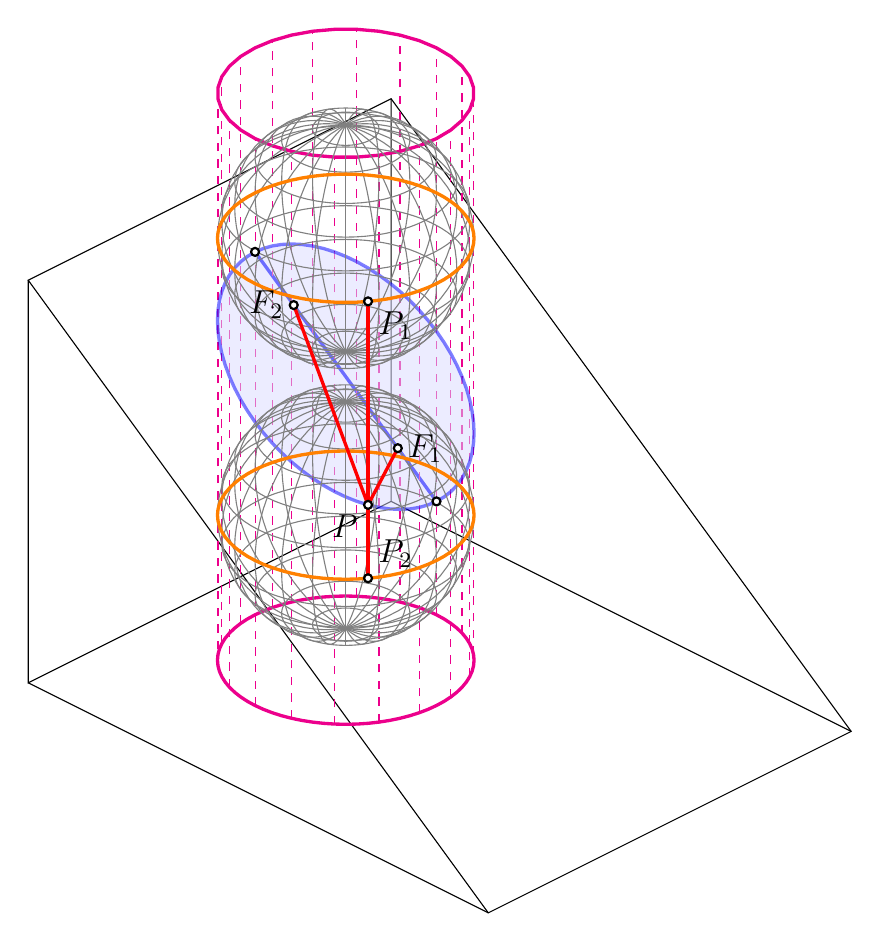
\begin{tikzpicture}[MyPersp,font=\large, scale=0.8]
		% the base circle is the unit circle in plane Oxy
		\def\h{2.5}% Heigth of the ellipse center (on the axis of the cylinder)
		\def\a{35}% angle of the section plane with the horizontal
		\def\aa{35}% angle that defines position of generatrix PA--PB
		\pgfmathparse{\h/tan(\a)}
	  \let\b\pgfmathresult
		\pgfmathparse{sqrt(1/cos(\a)/cos(\a)-1)}
	  \let\c\pgfmathresult %Center Focus distance of the section ellipse.
		\pgfmathparse{\c/sin(\a)}
	  \let\p\pgfmathresult % Position of Dandelin spheres centers
	                       % on the Oz axis (\h +/- \p)
		\coordinate (A) at (2,\b,0);
		\coordinate (B) at (-2,\b,0);
		\coordinate (C) at (-2,-1.5,{(1.5+\b)*tan(\a)});
		\coordinate (D) at (2,-1.5,{(1.5+\b)*tan(\a)});
		\coordinate (E) at (2,-1.5,0);
		\coordinate (F) at (-2,-1.5,0);
		\coordinate (CLS) at (0,0,{\h-\p});
		\coordinate (CUS) at (0,0,{\h+\p});
		\coordinate (FA) at (0,{\c*cos(\a)},{-\c*sin(\a)+\h});% Focii
		\coordinate (FB) at (0,{-\c*cos(\a)},{\c*sin(\a)+\h});
		\coordinate (SA) at (0,1,{-tan(\a)+\h}); % Vertices of the
	                                           % great axes of the ellipse
		\coordinate (SB) at (0,-1,{tan(\a)+\h});
		\coordinate (PA) at ({sin(\aa},{cos(\aa)},{\h+\p});
		\coordinate (PB) at ({sin(\aa},{cos(\aa)},{\h-\p});
		\coordinate (P) at ({sin(\aa)},{cos(\aa)},{-tan(\a)*cos(\aa)+\h});
	     % Point on the ellipse on generatrix PA--PB
	
		\draw (A)--(B)--(C)--(D)--cycle;
		\draw (D)--(E)--(F)--(C);
		\draw (A)--(E) (B)--(F);
		\draw[blue,very thick] (SA)--(SB);
	
	%	\coordinate (O) at (0,0,0);
	%	\draw[->] (O)--(2.5,0,0)node[below left]{x};
	%	\draw[->] (O)--(0,3,0)node[right]{y};
	%	\draw[->] (O)--(0,0,6)node[left]{z};
	
		\foreach \t in {20,40,...,360}% generatrices
			\draw[magenta,dashed] ({cos(\t)},{sin(\t)},0)
	      --({cos(\t)},{sin(\t)},{2.0*\h});
		\draw[magenta,very thick] (1,0,0) % lower circle
			\foreach \t in {5,10,...,360}
				{--({cos(\t)},{sin(\t)},0)}--cycle;
		\draw[magenta,very thick] (1,0,{2*\h}) % upper circle
			\foreach \t in {10,20,...,360}
				{--({cos(\t)},{sin(\t)},{2*\h})}--cycle;
		\fill[blue!15,draw=blue,very thick,opacity=0.5]
	     (0,1,{\h-tan(\a)}) % elliptical section
			\foreach \t in {5,10,...,360}
				{--({sin(\t)},{cos(\t)},{-tan(\a)*cos(\t)+\h})}--cycle;
	
		\foreach \i in {-1,1}{%Spheres!
			\foreach \t in {0,15,...,165}% meridians
				{\draw[gray] ({cos(\t)},{sin(\t)},\h+\i*\p)
					\foreach \rho in {5,10,...,360}
						{--({cos(\t)*cos(\rho)},{sin(\t)*cos(\rho)},
	          {sin(\rho)+\h+\i*\p})}--cycle;
				}
			\foreach \t in {-75,-60,...,75}% parallels
				{\draw[gray] ({cos(\t)},0,{sin(\t)+\h+\i*\p})
					\foreach \rho in {5,10,...,360}
						{--({cos(\t)*cos(\rho)},{cos(\t)*sin(\rho)},
	          {sin(\t)+\h+\i*\p})}--cycle;
				}
						\draw[orange,very thick] (1,0,{\h+\i*\p})% Equators
			\foreach \t in {5,10,...,360}
				{--({cos(\t)},{sin(\t)},{\h+\i*\p})}--cycle;
			}
		\draw[red,very thick] (PA)--(PB);
		\draw[red,very thick] (FA)--(P)--(FB);
	%	\fill[MyPoints] (CLS) circle (1pt);% center of lower sphere
	%	\fill[MyPoints] (CUS) circle (1pt);% center of upper sphere
		\fill[MyPoints] (FA) circle (1pt)node[right]{$F_1$};
		\fill[MyPoints] (FB) circle (1pt)node[left]{$F_2$};
		\fill[MyPoints] (SA) circle (1pt);
		\fill[MyPoints] (SB) circle (1pt);
		\fill[MyPoints] (P) circle (1pt)node[below left]{$P$};
		\fill[MyPoints] (PA) circle (1pt)node[below right]{$P_1$};
		\fill[MyPoints] (PB) circle (1pt)node[above right]{$P_2$};
	\end{tikzpicture}
	\end{center}
		\caption{Dudlin Sphere (source: Hugues Vermeiren)}
	\end{figure}
	Sorry for the reader that likes the Dudlin proof but we don't want to lose time by rewriting proofs just in another way and this especially with the \LaTeX{} langue script... (even if the proofs are small). 
	
	\subsubsection{Classification of conical by the determinant}
	For the purposes of the classification of the partial differential equations which we shall study in the section of Differential and Integral Calculus, let us return to the general equation of conics (with a $2$ factor on some terms to simplify the developments that will follow):
	
	with $(a,b,c)\neq (0,0,0)$. 

	We will try to classify the conics by using a purely matrix property and drawing inspiration from what has been seen previously.

	As we know, any $\Gamma$ of $\mathbb{R}^2$ admitting an equation of the above form is named a "conic".

	We have also show that we can rewrite the equation above as:
	
	with:
	
	and let us recall that we have proved in the Linear Algebra chapter that if is symmetric, there exists an orthogonal matrix $S$ (thus satisfying $S^TS=\mathds{1}$) such that:
	
 	where $\lambda$ and $\mu$ are the eigenvalues of $A$.

	Before proceeding, let us notice that by using one of the properties of the determinant demonstrated in the section of Linear Algebra we have:
	
	because:
	
	Therefore:
	
	\begin{tcolorbox}[title=Remark,colframe=black,arc=10pt]
	If we would not have introduce the factor $2$ at the beginning this would have been written:
	
	This is why a lot of textbooks classify the conic by multiplying the determinant by $4$ and to make an analogy to the distriminant of polynomial (it's more easy for the studenty to remember) they multiply it by $-1$ to get therefore the "\NewTerm{discriminant of conic sections}\index{discriminant of conic section}":
	
	\end{tcolorbox}
 	Now let us observe what happens as a function of the value of this determinant and therefore in extenso as a function of the components of the matrix $A$.

	There are two cases to consider from which only three a very exclusive:
	\begin{itemize}
		\item Case of a non-null determinant $\det(A)\neq 0$:
		In the case where $\det(A)\neq 0$, then we have then that is $A$ invertible (\SeeChapter{see demonstration Linear Algebra}). In order to simplify the equation:
		
	 	to make the term $X$ disappear in order to obtain something well known to us, we are going to seek to translate the curve (the choice of starting with a translation being the most trivial one). By a small trial and error, we find that it is enough to translate each point $X$ of the curve from an $Y$ worth:
		
		We then have as $(\vec{x}+\vec{y})\in \Gamma$:
		
	 	After simplification we get by using the associativity properties of the multiplication, the distributivity of the matrix addition and by remembering that for a symmetric matrix (\SeeChapter{see section Linear Algebra}):
		
		and also remembering that (see chapter of Linear Algebra):
		
		Then we have:
		
		To continue, remember that $\vec{x}$ and $B$ are vectors, then $\vec{x}^TB$ and $B^T\vec{x}$ are scalars that are equals and therefore cancel. It remains then to us:
		
		We can then say that the translated curve admits as equation:
	
	where obviously:
	
 	or what is explicitly equivalent to:
	
	We thus succeeded in simplifying the equation in the case where $A$ is invertible by removing the term in $\vec{x}$.

	The type of curve (ellipse, parabola, hyperbola, etc.) is obviously not changed by a translation, which is why we consider the previous equation to be the simplest equation.

	More generally, the type of curve is not changed by an orthogonal matrix (easy to see because the image of an orthonormal basis by an orthogonal matrix is still an orthonormal basis). Thus, by choosing to undergo an orthogonal transformation to $X$ by $S$ (which is an orthogonal matrix for information), we are then led to write:
	
	given that for recall that:
	
 	we deduce that:
	
	In conclusion, we can assert that the curve defined by the equation above is of the same type as the original curve $\Gamma$.

		\item Case of a strictly positive determinant $\det(A)>0$:
		
		In the case where $\det(A)>0$, that is to say $ac-b^2>0$ or equivalently as we have mention it the previous remark $b^2-4ac<0$, $\lambda$ and $\mu$ have the same sign as by construction and for recall:
		
		The relation:
		
		still remains valid in this situation.
	
		But, in function of the value of $C_1$ we have prove earlier above how to interpret this equation. That is for recall (don't forget that we are in the space of real numbers!):
		\begin{itemize}
			\item If $C_1$ has the same sign as $\lambda$ and $\mu$ the equation has nos solution and $\Gamma=0$
	
			\item If $C_1=0$ we see that the equation is reduced ton a point
	
			\item If $C_1$ has a sign opposed to $\lambda$ and $\mu$ then we recognized the equation of an ellipse
		\end{itemize}

		\item Case of a strictly negative determinant $\det(A)<0$:
		
		In the case where $\det(A)<0$, that is to say $ac-b^2<0$ or equivalently as we have mention it the previous remark $b^2-4ac>0$, $\lambda$ and $\mu$ have opposite signs as by construction and for recall:
		
		The relation:
		
		still remains valid in this situation.

		But, in function of the value of $C_1$ we have prove earlier above how to interpret this equation. That is for recall (don't forget that we are in the space of real numbers!):
		\begin{itemize}
			\item If $C_1=0$ then $\Gamma$ is the union of the secant lines
	
			\item If $C_1\neq 0$ we recognize the equation of a hyperbola
		\end{itemize}

		\item Case of a null determinant $\det(A)=0$:
		
		In the case where $\det(A)=0$, that is to say $ac-b^2=0$ or equivalently as we have mention it the previous remark $b^2-4ac=0$, one of the eigenvalues is equal to zero, for example $\mu=0$ (only only because we must have $A\neq 0$). As we know:
		
		and by the equation
		
		we then have:
		
		Therefore:
		
		By developing explicitly, we get:
		
		The latter equation can be rewritten as:
		
		with obviously:
		
		If $e=0$ we can have three situations:
		\begin{itemize}
			\item $C_2=0$, then $\Gamma$ is a straight line

			\item $C_2$ and $\lambda$ have the same signs the $\Gamma=\varnothing$

			\item $C_2$ and $\lambda$ are of opposite signs, then $\Gamma$ is the union of two parallel distinct straight lines
		\end{itemize}
		If $e\neq 0$, then $\Gamma$ is a parabola.
	\end{itemize}
	Let us make a summary of this classification:
	\begin{itemize}
		\item If $\det(A)=ac-b^2>0$ (or $b^2-4ac<0$), then $\Gamma$ is either empty, reduced to a point, or an ellipse

		\item If $\det(A)=ac-b^2<0$ (or $b^2-4ac>0$), then $\Gamma$ is either the intersection of two secant straight lines, or an hyperbola

			\item If $\det(A)=ac-b^2=0$ (or $b^2-4ac=0$), then $\Gamma$ is either empty, or the parallel straight lines, or a parabola
	\end{itemize}	

	\pagebreak
	\subsection{Parametrizations}
	Parametrization  is the process of deciding and defining the parameters necessary for a complete or relevant specification of a model or geometric object.
	
	Parametrization is also the process of finding parametric equations of a curve, a surface, or, more generally, a manifold or a variety, defined by an implicit equation. The inverse process is called "\NewTerm{implicitization}\index{implicitization}".
	
	Most often, parametrization is a mathematical process involving the identification of a complete set of effective coordinates or degrees of freedom of the system, process or model, without regard to their utility in some design. Parametrization of a line, surface or volume, for example, implies identification of a set of coordinates that allows one to uniquely identify any point (on the line, surface, or volume) with an ordered list of numbers. Each of the coordinates can be defined parametrically in the form of a parametric curve (one-dimensional) or a parametric equation (2+ dimensions).
	
	Generally, the minimum number of parameters required to describe a model or geometric object is equal to its dimension, and the scope of the parameters—within their allowed ranges—is the parameter space.
	
	\begin{tcolorbox}[title=Remark,colframe=black,arc=10pt]
		Parametrizations are not unique. The ordinary three-dimensional object can be parametrized (or coordinatized) equally efficiently with Cartesian coordinates, cylindrical polar coordinates, spherical coordinates or other coordinate systems (\SeeChapter{see section Vector Calculus}").
	\end{tcolorbox}
	As notice above for some of the forms described below, it is possible to select a different coordinate than the Cartesian coordinates such as, for example cylindrical or spherical coordinates which are in some cases much simpler to implement. We will try as far as possible to present the most important one.
	
	\subsubsection{Equation of the Plane}
	Given a plane $P$ for which we know a normal and unit vector $\vec{n}(a,b,c)$ but not the equation and $A(x,y,z)$ a point of the plane $P$.
	
	\begin{tcolorbox}[title=Remark,colframe=black,arc=10pt]
	If we don't have $\vec{n}$ but instead three points of the plane $P_1(x_1,y_1,z_1),P_2(x_2,y_2,z_2),P_3(x_3,y_3,z_3)$ we easily get  $\vec{n}$ by calculating the cross product:
	
	\end{tcolorbox}
	
	For a point $M$ with coordinates $(x, y, z)$ belongs to the plane $P$ it is necessary and sufficient that the vectors $\overrightarrow{AM}$ and $\vec{n}$ are orthogonal.
	
	So given the point by the vector $\overrightarrow{AM}$ of coordinates:
	
	If $\overrightarrow{AM}$ is perpendicular to $\vec{n}$ then the dot product must be zero as:
	
	Which can also be written as:
	
	such that we get the general Cartesian equation of the plane:
	
	This equation where $(a,b,c)\cong (0,0,0)$ that checks that the coordinates of any point $M(x,y,z)$ belongs to the plan $P$ is therefore named "\NewTerm{Cartesian equation of the plane $P$}\index{Cartesian equation of a plane}".
	
	If we write the equation with the direction cosines of $\vec{n}$ (\SeeChapter{see section Calculus Vector}), we therefore have also:
	
	\begin{tcolorbox}[title=Remark,colframe=black,arc=10pt]
	To get a cube in space, with only need six planes delimited by conditions such as $x\leq...,y\leq...,z\leq...$.
	\end{tcolorbox}	
	It is relatively easy to go from case by case from the Cartesian equation of the plane to the parametric equation of the plane. We can (with the usual precautions ...) resume the equation:
	
	and rewriting it as follows:
	
	and therefore, the parametric equation of the plane in the space of dimension $3$ will be written:
	
	\begin{tcolorbox}[colframe=black,colback=white,sharp corners]
	\textbf{{\Large \ding{45}}Example:}\\\\
	With Maple 4.00b:\\

	\texttt{>a:=3:b:=-2:c:=1:d:=5:\\
	>plot3d([x,y,(-d-b*y+a*x)/c],x=-2..2,y=-2..2, orientation=[-87,81],style=PATCH,
axes=NORMAL);
	}
	\begin{figure}[H]
		\centering
		\includegraphics{img/geometry/plane.jpg}
		\caption{Example of plane with Maple 4.00b}
	\end{figure}
	\end{tcolorbox}
	In perspective geometry (see section of the same name) an important case to consider is the plane of perpendicular to the $\vec{n}=(1,1,1)$ that give the isometric perspective that keeps lengths of cube of equal size (this plane being assimilated to the table of the observer):
	\begin{figure}[H]
		\centering
		\includegraphics{img/geometry/isometric_perspective_plane.jpg}
	\end{figure}

	So using the previous relation we get:
	
	Now to calculate the angle between this plane and the $xy$-plane we calculate the dot product between the respective normal vectors and subtract $\pi$ such that:
	
	Thus:
	
	 Therefore:
	
	 Therefore the angle $\beta$ between the two planes is in degrees (as it is usage in perspective geometry to work in degrees):
	 
	 That is perspective geometry is rounded to the famous $30^\circ$
	
	\pagebreak	
	\subsubsection{Equation of the Straight line}
	As we saw it in the section of Functional Analysis, a straight line in the plane can be described by the function:
	
	and we have also proved how to determine the equation of the mediator of two points in the plane (we had mentioned also that the proof was more on the order of Analytic Geometry as Functional Analysis).
	
	The general Cartesian equation of the straight line is then simply given by:
	
	or sometimes:
	
	Indeed, simplifying we fall back on the "\NewTerm{reduced Cartesian equation}\index{reduced Cartesian equation of a line}":
	
	with by definition:
	
	We also saw in the section Calculus that straight lines with inequalities rather than strict equalities gives the possibility to define special areas on the plane:
	\begin{center}
	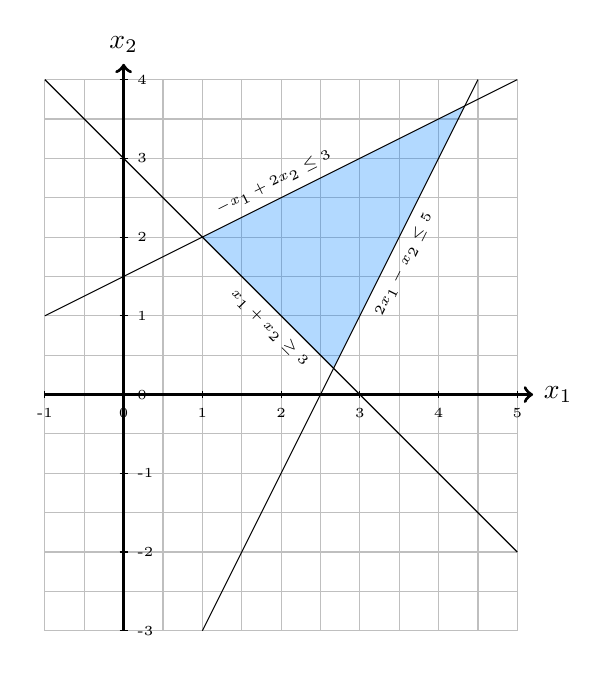
\begin{tikzpicture}

    \draw[gray!50, thin, step=0.5] (-1,-3) grid (5,4);
    \draw[very thick,->] (-1,0) -- (5.2,0) node[right] {$x_1$};
    \draw[very thick,->] (0,-3) -- (0,4.2) node[above] {$x_2$};

    \foreach \x in {-1,...,5} \draw (\x,0.05) -- (\x,-0.05) node[below] {\tiny\x};
    \foreach \y in {-3,...,4} \draw (-0.05,\y) -- (0.05,\y) node[right] {\tiny\y};

    \fill[blue!50!cyan,opacity=0.3] (8/3,1/3) -- (1,2) -- (13/3,11/3) -- cycle;

    \draw (-1,4) -- node[below,sloped] {\tiny$x_1+x_2\geq3$} (5,-2);
    \draw (1,-3) -- (3,1) -- node[below left,sloped] {\tiny$2x_1-x_2\leq5$} (4.5,4);
    \draw (-1,1) -- node[above,sloped] {\tiny$-x_1+2x_2\leq3$} (5,4);

	\end{tikzpicture}
	\end{center}
	\textbf{Definition (\#\mydef):} We name "\NewTerm{direction vector}\index{direction vector}" of a line $(D)$, all non-zero vector in the same direction as the straight line.
	
	Let us now prove two small friendly theorems:
	\begin{theorem}
	If a line has for equation $y=ax+b$ then the vector:
	
	is a direction vector for this line.
	\end{theorem}
	\begin{dem}
	Given $D:ax+b$ and $A, B$, two points of this line taken such as ${A(0,b),B(1,a+b)}$. Since $A, B$ are two points $D$ then $\overrightarrow{AB}$ is a direction vector of $D$ then:
	
	On the way a small interesting corollary that has an application in physics!:
	
	If a straight line $D_1$ has direction vector being:
	
	and another straight line $D_2$ with a direction vector being:
	
	therefore their scalar product (\SeeChapter{see section Vector Calculus}) is zero:
	
	that shows that two straight lines wich multiplication of slopes (second coordinate of the direction vector) is equal to $-1$ are perpendicular!
	\begin{flushright}
		$\square$  Q.E.D.
	\end{flushright}
	\end{dem}
	\begin{theorem}
	If a line has for equation $ax+by+c=0$ then the vector:
	
	is a direction vector for this line.
	\end{theorem}
	\begin{dem}
	Given:
	
	therefore:
	
	then the vector:
	
	is a direction vector $D$ and any vector:
	
	with $\alpha\in \mathbb{R}$.
	Thus, there are infinite ways to define the same line, because the line is composed of an infinite number of points (all of which can serve as an anchor point) and there is an infinity of multiple direction vector!
	\begin{flushright}
		$\square$  Q.E.D.
	\end{flushright}
	\end{dem}
	
	\pagebreak
	\paragraph{Distance from a line to a point}\mbox{}\\\\
	Often we seek the distance between a line and a point external to it. Thus, consider the following figure:
	\begin{figure}[H]
		\centering
		\includegraphics{img/geometry/point_to_line.jpg}
		\caption{Representation of the search of the distance from a point to a line}
	\end{figure}
	With the point $H$ the orthogonal projection of $A$ on the straight line $d$, $P$ an arbitrary point of the straight line $d$ and $\vec{n}$ anj orthogonal vector (normal) to $d$.
	
	We have (\SeeChapter{see section Vector Calculus}):
	
	As $\alpha=0$ or $\alpha=\pi$. Therefore:
	
	where $\delta$ is the distance (we can note denote the distance with the letter $d$ as we did at the beginning of this chapter, otherwise there would be confusion a with the $d$ chosen to represent the straight right in this development).
	
	So we get the relation:
	
	Consider now explicitly the point $A(x_0,y_0)$ and the striaght line equation: $d:ax+by+c=0$.
	
	Let us choose a point $P\in d:P(0,-c/b)$ and a vector normal $\vec{n}$, normal to $d:\vec{n}\begin{pmatrix}a \\ b\end{pmatrix}$. Indeed, as we have proven just before that:
	
	is a direction vector of a straight line $D$ we have well:
	
	and thus $\vec{v}$ and $\vec{n}$ are perpendicular.
	
	Thus, by applying the previous relation, we have:
	
	and therefore:
	
	
	\paragraph{Line defined by the intersection of planes}\mbox{}\\\\
	If we now consider two non-parallel planes in space, their intersection is a straight line. Indeed, consider two planes of respective equations:
	
	and $D$ and their straight line of intersection.
	
	Obviously a point $M(x_0,y_0,z_0)$ in space is located on the straight line $D$ if and only if the point $M$ satisfies the system of equations:
	
	An example with images and numerical application is given in the section of Theoretical Computing.
	\begin{tcolorbox}[title=Remark,colframe=black,arc=10pt]
	While in $\mathbb{R}^2$ a straight line is fully characterized by an equation of the type $ax+by+c=0$, in space, a single equation of the form $ax+by+cz+d=0$ obviously characterizes a plan. To characterize a straight line outside of the planes of the axes, it is necessary (parametric equation apart) to have two equations of planes.
	\end{tcolorbox}	
	
	\paragraph{Parametric equation of a line in $\mathbb{R}^3$}\mbox{}\\\\
	It is relatively trivial (but we will still prove it) that the parametric equation in $\mathbb{R}^3$ of a straight line is a kind of system of equations:
	
	Thus, each component increases linearly with respect to the same variable to a constant and a factor. This can also be written in vector form (more traditional):
	\begin{equation}
  \addtolength{\fboxsep}{5pt}
   \boxed{
   \begin{gathered}
   		\begin{pmatrix}
   		x(t)\\y(t)\\z(t)
   		\end{pmatrix}=
   		\begin{pmatrix}
   		a\\c\\c
   		\end{pmatrix}t+\begin{pmatrix}
   		\alpha\\ \beta \\ \gamma
   		\end{pmatrix}
   \end{gathered}
   }
	\end{equation}
	The vector $\vec{v}=(a,b,c)$ is obviously named the "direction vector".
	\begin{dem}
	So we have the system of equations (two equations with three unknowns, and therefore one unknown will be indeterminate):
	
	Let us eliminate one of the variables (arbitrarily we start with $z$):
	
	where $\alpha=c/c'$ therefore:
	
	So (it's a little stupid to write but...):
	
	Similarly with $y$ such that $\beta=b/b'$ we have:
	
	Therefore:
	
	Finally we have:
	
	The direction vector and the vector or ordinates have all constant components. This allows us to write more generally:
	
	\begin{flushright}
		$\square$  Q.E.D.
	\end{flushright}
	\end{dem}
	\begin{tcolorbox}[title=Remarks,colframe=black,arc=10pt]
	\textbf{R1.} The equation of a straight line is almost one of the most important thing in the synthesis of 3D images because from this latter we can build polygons and assemble them to build more complex three-dimensional shapes.\\
	
	\textbf{R2.} As already seen before with an example, to determine if a line is perpendicular to a plane we must determine at least two intersecting lines in the same plane and perform the cross product of their direction vector and then calculate the dot product between the result of the vector product and the first straight light for which we seek the orthogonality. Indeed, a straight single of the plane does not permit to determine the orientation of the latter; wee need a least two straight lines.
	\end{tcolorbox}
	
	\subsubsection{Equation of a Square}
	In 1992, Manuel Fernandez Guasti introduced an algebraic equation for representing an intermediate shape between the circle and the square. His equation included a parameter $s$ that can be used to blend the circle and the square smoothly thanks to a quite simple equation named "\NewTerm{FG-squircle}\index{FG-squircle}" and given by:
	
	The squareness parameter $s$ can have any value between $0$ and $1$. When $s = 0$, the equation produces a circle with radius $k$. When $s = 1$, the equation produces a square with a side length of $2k$. In between, the equation produces a smooth curve that interpolates between the two shapes.
	
	We will focus here to the case $k=s=1$ that gives therefore::
	
	and when $-1<x<1$ and $-1<y<1$ this corresponds to a square centered and the origin. Indeed with Maple:
	
	\texttt{>with(plots):\\
	>implicitplot(x\string^2+y\string^2-x\string^2*y\string^2= 1,x=-1..1,y=-1..1);
	}
	\begin{figure}[H]
		\centering
		\includegraphics{img/geometry/fg_squircle.jpg}
		\caption{FG-squircle reprsentation in Maple 4.00}
	\end{figure}

	This implicit equation of the square will be useful to us to study the isomorophism of a circle and a square in the section Topology.
	
	\subsubsection{Equation of a Cycloid}
	A cycloid is the curve traced by a point on the rim of a circular wheel as the wheel rolls along a straight line without slippage. It is an example of a roulette, a curve generated by a curve rolling on another curve.

	The cycloid is an important curve in physics! Indeed as we will prove it in the section of Classical Mechanics, tec cycloid, with the cusps pointing upward, is the curve of fastest descent under constant gravity, and is also the form of a curve for which the period of an object in descent on the curve does not depend on the object's starting position.

	\begin{center}
	  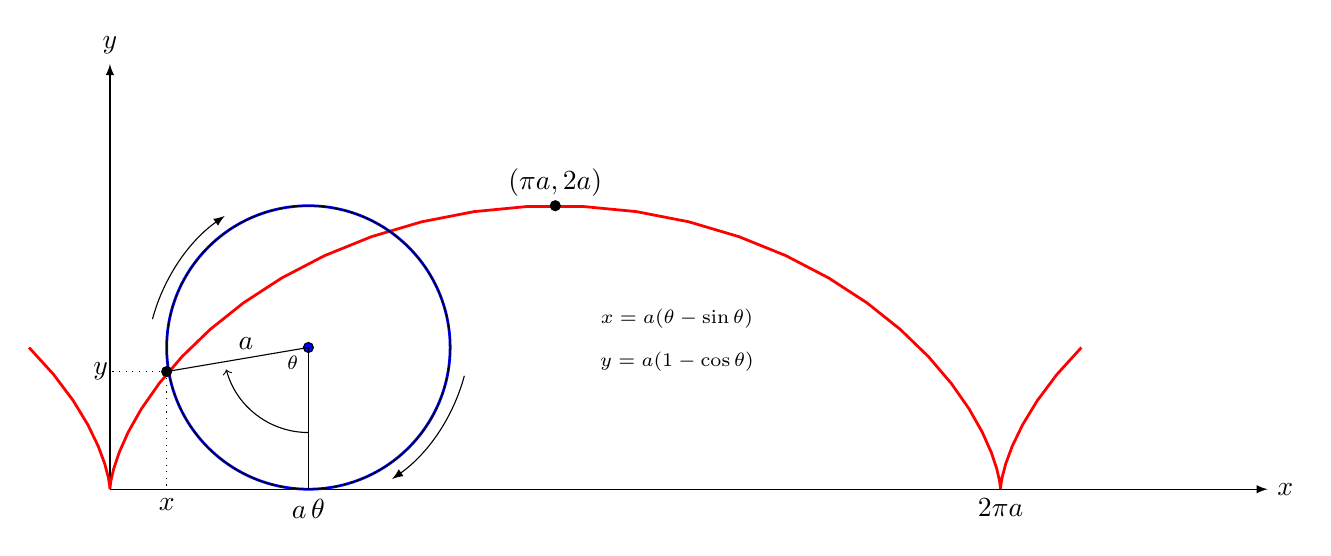
\begin{tikzpicture}[scale=1.8]
	  \coordinate (O) at (0,0);
	  \coordinate (A) at (0,3);
	  \def\r{1} % radius
	  \def\c{1.4} % center
	  \coordinate (C) at (\c, \r);
	
	
	  \draw[-latex] (O) -- (A) node[anchor=south] {$y$};
	  \draw[-latex] (O) -- (2.6*pi,0) node[anchor=west] {$x$};
	  \draw[red,domain=-0.5*pi:2.5*pi,samples=50, line width=1] 
	       plot ({\x - sin(\x r)},{1 - cos(\x r)});
	  \draw[blue, line width=1] (C) circle (\r);
	  \draw[] (C) circle (\r);
	
	  % coordinate x 
	  \def\x{0.4} % coordinate x
	  \def\y{0.83} % coordinate y
	  \def\xa{0.3} % coordinate x for arc left
	  \def\ya{1.2} % coordinate y for arc left
	  \coordinate (X) at (\x, 0 );
	  \coordinate (Y) at (0, \y );
	  \coordinate (XY) at (\x, \y );
	
	  \node[anchor=north] at (X) {$x$} ;
	
	  % draw center of circle
	  \draw[fill=blue] (C) circle (1pt);
	
	  % draw radius of the circle
	  \draw[] (C) -- node[anchor=south] {\; $a$} (XY);
	
	  % bottom of circle, radius to the bottom
	  \coordinate (B) at (\c, 0);
	  \draw[] (C) -- (B) node[anchor=north] {$a \, \theta$};
	
	  % projections of point XY
	  \draw[dotted] (XY) -- (X);
	  \draw[dotted] (XY) -- (Y) node[anchor=east, xshift=1mm] {$\quad y$};
	
	  % arc theta
	  % start arc
	  \coordinate (S) at (\c, 0.4);
	  \draw[->] (S) arc (-90:-165:0.6);
	  \node[xshift=-2mm, yshift=-2mm] at (C) {\scriptsize $\theta$};
	
	  % arc above
	  \coordinate (AA) at (\xa, \ya);
	  \draw[-latex, rotate=25] (AA) arc (-220:-260:1.3);
	
	  % arc below
	  \def\xb{2.5} % coordinate x for arc bottom
	  \def\yb{0.8} % coordinate y for arc bottom
	  \coordinate (AB) at (\xb, \yb);
	  \draw[-latex, rotate=-10] (AB) arc (-5:-45:1.3);
	
	  % XY dot
	  \draw[fill=black] (XY) circle (1pt);
	
	  % top label
	  \coordinate (T) at (pi, 2);
	  \node[anchor=south] at (T)  {$(\pi a, 2 a )$} ;
	  \draw[fill=black] (T) circle (1pt);
	
	  % equations
	  \coordinate (E) at ( 4,1.2);
	  \coordinate (F) at ( 4,0.9);
	  \node[] at (E) {\scriptsize $x=a(\theta - \sin \theta)$};
	  \node[] at (F) {\scriptsize $y=a(1 - \cos \theta)$};
	
	  % label 2pi a
	  \coordinate (TPA) at (2*pi, 0);
	  \node[anchor=north] at (TPA) {$2 \pi a$};
	
	  \end{tikzpicture}
	\end{center}
	We see on the figure above that as an arc $\theta$ of the circle of radius $a$ has a length
	
	This corresponds to the abscissa distance in the range $[0,2\pi a]$.
	
	But to get the $x$  value of the tracked point we must subtract the horizontal projection $a'$ of the radius $a$ on the abscissa and as:
	
	Therefore:
	
	And the same procedure applies for $y$.

	So we finally get:
	
	
	\subsubsection{Equation of an Epicycloid}
	In geometry, an epicycloid is a plane curve produced by tracing the path of a chosen point on the circumference of a circle - named an "epicycle" - which rolls without slipping around a fixed circle. It is a particular kind of roulette.
	\begin{figure}[H]
		\centering
		\includegraphics{img/geometry/epicycloid_path.jpg}
		\caption{Epicycloid path (source: Wikipedia, Sam Derbyshire)}
	\end{figure}
	As we will see in the section of Mechanical Engineering, the epicycloid is used to build efficient energy gearing geometry shapes!
	
	For the need of the section of Mechanical Engineering we need to determine the parametric equation of the epicycloid . For this consider the following figure:
	\begin{figure}[H]
		\centering
		\includegraphics[scale=0.6]{img/geometry/epicycloid_sketch_for_proof.jpg}
		\caption{Epicycloid sketch for proof (source: Wikipedia, Sam Derbyshire)}
	\end{figure}
	We assume that the position of $P$ is what we want to solve, {$\alpha$  is the radian from the tangential point to the moving point $P$, and $\theta$  is the radian from the starting point to the tangential point.

	Since there is no sliding between the two cycles, then we have that:
	
	By the definition of radian (which is the rate arc over radius), then we have that:
		
	From these two conditions, we get the identity:
	
	By rearranging, we get the relation between $\alpha$  and $\theta$, which is
	
	From the figure, we see the position of the point $P$ is clearly given by:
	
	
	\subsubsection{Equation of an Hypocycloid}
	In geometry, a hypocycloid is a special plane curve generated by the trace of a fixed point on a small circle that rolls within a larger circle. It is comparable to the cycloid or epicycloid but instead of the circle rolling along a line, it rolls within a circle.
	\begin{figure}[H]
		\centering
		\includegraphics{img/geometry/hipocycloid_path.jpg}
		\caption{Hypocycloid path (source: Wikipedia, Sam Derbyshire)}
	\end{figure}
	When we know the parametric equation of the epicycloid, that of the hypocycloid is immediate:
	
	Now for the section of Mechanical Engineering it will help if the reader compare side by side and epicycloid and a hypocycloid one:
	\begin{figure}[H]
		\centering
		\begin{subfigure}{.4\textwidth}
		  \centering
		  \includegraphics[scale=0.9]{img/geometry/epicycloid.jpg}
		  \caption{Epicycloid (source: Wikipedia)}
		\end{subfigure}
		\begin{subfigure}{.4\textwidth}
		  \centering
		  \includegraphics[scale=1]{img/geometry/hipocycloid.jpg}
		  \caption{Hipocycloid}
		\end{subfigure}
	\end{figure}
		
	
	
	\pagebreak
	\subsubsection{Surface of revolution}
	More generally many surfaces (and also some of which we've seen before as the sphere, tore and cylinder) can be described by revolving a primary form of smaller size and then by rotation.
	
	\textbf{Definition (\#\mydef):} A "\NewTerm{surface of revolution}\index{surface of revolution}" is a surface obtained by rotating a plane curve (e.g. $z=f(x)$), named the "\NewTerm{generatrix}\index{generatrix}", around the $z$-axis (for example!). So we pass from a plane of $\mathbb{R}^2$ to a basis in $\mathbb{R}^3$, the $x$-axis then generates a plane that has become the $y$O$z$ plane.
	\begin{figure}[H]
		\centering
		\includegraphics[scale=0.85]{img/geometry/revolution_surface.jpg}
	\end{figure}
	Let us see seven famous cases:
	
	\paragraph{Cone}\mbox{}\\\\
	Consider a circular cone of vertex O (origin) with a circle of center $(0,0, h)$ (where $h$ is a positive real number corresponding to the height of the) and radius $R$:
	\begin{figure}[H]
		\centering
		\includegraphics{img/geometry/cone.jpg}
		\caption{Representation of a cone}
	\end{figure}
	A parametric representation of the circle at the height $h$ is given as we already proved earlier by:
	
	where $t$ belongs to the interval $[-\pi,\pi]$.
	
	By extension, the parametric representation of a cone is:
	
	this can also be written in vector form (more traditional):
	\begin{equation}
	  \addtolength{\fboxsep}{5pt}
	   \boxed{
	   \begin{gathered}
	   		\begin{pmatrix}
	   		x(t,k)\\y(t,k)\\z(t,k)
	   		\end{pmatrix}=
	   		\begin{pmatrix}
	   		kr\cos(t)\\kr\sin(t)\\kh
	   		\end{pmatrix}
	   \end{gathered}
	   }
	\end{equation}
	
	In other words, the circle linearly propagates in all directions.
	\begin{tcolorbox}[colframe=black,colback=white,sharp corners]
	\textbf{{\Large \ding{45}}Example:}\\\\
	With Maple 4.00b:\\

	\texttt{>r:=1:h:=4:\\
	>plot3d([k*r*cos(t),k*r*sin(t),k*h],k=0..10,t=0..2*Pi,\\
	orientation=[50,60],style=PATCH,axes=NORMAL);
	}
	\begin{figure}[H]
		\centering
		\includegraphics{img/geometry/cone_maple.jpg}
		\caption{Parametric representation of a cone with Maple 4.00b}
	\end{figure}
	\end{tcolorbox}
	This suggests also the following cartesian equation of this cone:
	
	As we have $\tan(\alpha)=r/h$ we can write:
	
	Therefore:
	
	which is the Cartesian equation of a cone in space that we will see again in the section of Special Relativity in our study of light cones.
	
	\paragraph{Sphere}\mbox{}\\\\
	Consider the orthonormal basis ${\vec{i},\vec{j},\vec{k}}$, Given the sphere $S^2$ of  center $\Omega(a,b,c)$ and of radius $r$:
	\begin{figure}[H]
		\centering
		\includegraphics{img/geometry/sphere.jpg}
		\caption{Representation of a sphere}
	\end{figure}
	$M(x,y,z)$ belongs to the sphere  $S^2$ of radius $r$ fi and only if:
	
	that is to say by applying Pythagoras theorem:
	
	Hence the "\NewTerm{Cartesian equation of the sphere}\index{Cartesian equation of the sphere}" in the basis ${\vec{i},\vec{j},\vec{k}}$:
	
	There is another way to describe the sphere using the parametric equation. Indeed, we saw in the section of Vector Calculus that the transformation of the Cartesian coordinates to spherical coordinates is given by the following curvilinear coordinates:
	
	Therefore we have well (by a change of variable this also represent a sphere not centered at the origin):
	
	So the parametric equation of the sphere is well:
	\begin{equation}
	  \addtolength{\fboxsep}{5pt}
	   \boxed{
	   \begin{gathered}
	   		\begin{pmatrix}
	   		x(\theta,\phi)\\y(\theta,\phi)\\z(\theta,\phi)
	   		\end{pmatrix}=
	   		\begin{pmatrix}
	   		r\sin(\theta)\cos(\phi)\\r\sin(\theta)\sin(\phi)\\r\cos(\theta)
	   		\end{pmatrix}
	   \end{gathered}
	   }
	\end{equation}
	We fall back therefore on the Cartesian equation of a sphere to a given translation constant.
	\begin{tcolorbox}[colframe=black,colback=white,sharp corners]
	\textbf{{\Large \ding{45}}Example:}\\\\
	With Maple 4.00b for a sphere of unit radius:\\

	\texttt{>r:=1:h:=4:\\
>plot3d([sin(theta)*cos(phi),sin(theta)*sin(phi),cos(theta)],\\
theta=0..Pi,phi=-Pi..Pi,scaling=CONSTRAINED,orientation=[50,60],\\
style=PATCH,axes=NORMAL);
	}
	\begin{figure}[H]
		\centering
		\includegraphics{img/geometry/sphere_maple.jpg}
		\caption{Parametric representation of a sphere with Maple 4.00b}
	\end{figure}
	\end{tcolorbox}
	
	\subparagraph{Great circle of sphere}\mbox{}\\\\
	We will introduce here a concept that will be useful to us when we will study the geodesic of a sphere in the section of Analytical Mechanics.
	
	\textbf{Definition (\#\mydef):}  A "\NewTerm{great circle}\index{great circle}", also known as an "\NewTerm{orthodrome}\index{orthodrome}" or "\NewTerm{Riemannian circle}\index{Riemannian circle}", of a sphere is the intersection of the sphere and a plane that passes through the center point of the sphere. This partial case of a circle of a sphere is opposed to a "\NewTerm{small circle}\index{small circle}", the intersection of the sphere and a plane that does not pass through the center. Any diameter of any great circle coincides with a diameter of the sphere, and therefore all great circles have the same circumference as each other, and have the same center as the sphere. A great circle is the largest circle that can be drawn on any given sphere. Every circle in Euclidean 3-space is a great circle of exactly one sphere.
	\begin{figure}[H]
		\centering
		\includegraphics[scale=0.5]{img/geometry/great_circle.jpg}
		\caption{A great circle divides the sphere in two equal hemispheres}
	\end{figure}
	Let use choose now unit normal vector to a plane passing through the origin using Euler angles be
	
	where for rotated our such that the component $n_2$ is equal to $0$ (as it is always possible to do so whatever the plan we choose that pass through the origin!).
	
	If we choose a sphere of radius $r=1$ such that it's parametric equation is written as:
	
	And as the set of points that are at the interesection of the plane and the sphere are by construction such that:
	
	Therefore we get:
	
	After rearranging:
	
	Let us put:
	
	and using the definition of the cotangent:
	
	This is therefore the "\NewTerm{equation of a great circle}\index{equation of a great circle}".
	
	\pagebreak
	\paragraph{Ellipsoid (spheroid, geoid)}\mbox{}\\\\
	We saw in our study of conic that the cartesian equation of an ellipse in the plane was given by:
	
	with $a, b$ the two axes of the ellipse (small and large one).
	
	Thus, without rigorous proof, we can verify by hand or using computers that the Cartesian equation:
	
	is an ellipsoid:
	\begin{figure}[H]
		\centering
		\includegraphics{img/geometry/ellipsoid.jpg}
		\caption{Representation of an ellispoid}
	\end{figure}
	However, there is another way of describing an ellipsoid using also curvilinear coordinates:
	
	So the parametric equation of an ellipsoid will be:
	\begin{equation}
	  \addtolength{\fboxsep}{5pt}
	   \boxed{
	   \begin{gathered}
	   		\begin{pmatrix}
	   		x(\theta,\phi)\\y(\theta,\phi)\\z(\theta,\phi)
	   		\end{pmatrix}=
	   		\begin{pmatrix}
	   		a\cos(\theta)\cos(\phi)\\b\cos(\theta)\sin(\phi)\\c\sin(\theta)
	   		\end{pmatrix}
	   \end{gathered}
	   }
	\end{equation}
	We can see that this is simply the parametric equation of a sphere but with different radii along the axes of the chosen basis.
	\begin{tcolorbox}[colframe=black,colback=white,sharp corners]
	\textbf{{\Large \ding{45}}Example:}\\\\
	With Maple 4.00b:\\

	\texttt{>a:=100:b:=2:c:=20:\\
>plot3d([a*cos(theta)*cos(lambda),b*cos(theta)*sin(lambda),\\
c*sin(theta)],lambda=0..Pi,theta=-Pi..Pi,orientation=[50,60],\\
style=PATCH,axes=NORMAL);
	}
	\begin{figure}[H]
		\centering
		\includegraphics{img/geometry/ellipsoid_maple.jpg}
		\caption{Parametric representation of an ellipsoid with Maple 4.00b}
	\end{figure}
	\end{tcolorbox}
	So we have:
	
	hence:
	
	Finally:
	
	Is astronomy (\SeeChapter{see section Astronomy}) the ellipsoid is mainly named "\NewTerm{oblate spheroid}\index{oblate spheroid}".
	\begin{figure}[H]
		\centering
		\includegraphics{img/geometry/spheroid.jpg}
		\caption{Left oblate spheroid, right prolate spheroid (source: Wikipedia)}
	\end{figure}
	and we have technically a oblate spheroid when $c<a$ and prolate one when $c>a$. Obviously the case $a = c$ reduces to a sphere.
	
	\begin{tcolorbox}[title=Remark,colframe=black,arc=10pt]
	Because of the combined effects of gravity and rotation, the Earth's shape is not quite a sphere but instead is slightly flattened in the direction of its axis of rotation. For that reason, in cartography the Earth is often approximated by an oblate spheroid instead of a sphere. The current World Geodetic System model uses a spheroid whose radius is $6,378.137$ [km] at the equator and $6,356.752$ [km] at the poles.
	\end{tcolorbox}
	The aspect ratio of an oblate spheroid/ellipse, $b : a$, is the ratio of the polar to equatorial lengths, while the flattening (also named "oblateness") $f$, is the ratio of the equatorial-polar length difference to the equatorial length:
	
	
	\pagebreak
	\paragraph{Cylinder}\mbox{}\\\\
	It goes without saying that the parametric equation of a cylinder of radius $r$ is given by:
	\begin{equation}
	  \addtolength{\fboxsep}{5pt}
	   \boxed{
	   \begin{gathered}
	   		\begin{pmatrix}
	   		x(\phi)\\y(\phi)\\z
	   		\end{pmatrix}=
	   		\begin{pmatrix}
	   		r\cos(\phi)\\r\sin(\phi)\\z
	   		\end{pmatrix}
	   \end{gathered}
	   }
	\end{equation}
	We see well that the components $x, y$ satisfy the Cartesian equation of a circle for every $z$ since:
	
	\begin{tcolorbox}[colframe=black,colback=white,sharp corners]
	\textbf{{\Large \ding{45}}Example:}\\\\
	With Maple 4.00b a cylinder of radius $r=1$:\\

	\texttt{>plot3d([cos(phi),sin(phi),z],phi=-Pi..Pi,z=0..2,orientation=[50,60],\\
	style=PATCH,axes=NORMAL);
	}
	\begin{figure}[H]
		\centering
		\includegraphics{img/geometry/cylinder.jpg}
		\caption{Parametric representation of a cylinder with Maple 4.00b}
	\end{figure}
	\end{tcolorbox}
	It is obvious that the parametric equation of an elliptical base cylinder is given by:
	\begin{equation}
	  \addtolength{\fboxsep}{5pt}
	   \boxed{
	   \begin{gathered}
	   		\begin{pmatrix}
	   		x(\phi)\\y(\phi)\\z
	   		\end{pmatrix}=
	   		\begin{pmatrix}
	   		a\cos(\phi)\\b\sin(\phi)\\z
	   		\end{pmatrix}
	   \end{gathered}
	   }
	\end{equation}
	which also satisfies the parametric equation of an ellipse in the plane:
	
	
	\pagebreak
	\paragraph{Paraboloid}\mbox{}\\\\
	Given the equation of the parabola around the $z$-axis:
	
	with for reminder:
	
	We have obviously (by cutting the paraboloid py a horizontal plane wich gives therefore a circle of radius $r$) the relation:
	
	named "\NewTerm{cylinder equation}\index{cylinder equation}". But we also have by applying the Pythagorean theorem in the circle above:
	
	Therefore:
	
	Hence we get the "\NewTerm{Cartesian equation of the paraboloid (of revolution)}\index{Cartesian equation of the paraboloid }":
	
	We build the parametric equation of the paraboloid exactly in the same way as for the cone, at the difference that the evolution along the $z$-axis will not be linear relatively to a parameter $k$ but to the square of the latter. Therefore we have:
	\begin{equation}
	  \addtolength{\fboxsep}{5pt}
	   \boxed{
	   \begin{gathered}
	   		\begin{pmatrix}
	   		x(t,k)\\y(t,k)\\z(k)
	   		\end{pmatrix}=
	   		\begin{pmatrix}
	   		kr\cos(t)\\kr\sin(t)\\kh^2
	   		\end{pmatrix}=
	   		\begin{pmatrix}
	   		k\dfrac{1}{2p}\cos(t)\\k\dfrac{1}{2p}\sin(t)\\kh^2
	   		\end{pmatrix}
	   \end{gathered}
	   }
	\end{equation}
	\begin{tcolorbox}[colframe=black,colback=white,sharp corners]
	\textbf{{\Large \ding{45}}Example:}\\\\
	With Maple 4.00b a paraboloid with $h=1,p=1$:\\

	\texttt{>p:=1:h:=1:\\
	>plot3d([k*1/(2*p)*cos(t),k*1/(2*p)*sin(t),k\string^2*h],k=0..10,\\
	t=0..2*Pi,orientation=[50,60],style=PATCH,axes=NORMAL); 
	}
	\begin{figure}[H]
		\centering
		\includegraphics{img/geometry/paraboloid.jpg}
		\caption{Parametric representation of a paraboloid with Maple 4.00b}
	\end{figure}
	\end{tcolorbox}
	
	\pagebreak
	\paragraph{Hyperboloid}\mbox{}\\\\
	Given the linear function:
	
	that we turn around the $z$-axis. As the line passe trough the origin, the revolution around the $z$-axis is similar to two cones facing each other with their apex at the origin O. Therefore:
	
	which give us obviously:
	
	\textbf{Definition (\#\mydef):} Any surface generated by a line is a "\NewTerm{ruled surface}\index{ruled surface}". More explicitly a surface $S$ is ruled if through every point of $S$ there is a straight line that lies on $S$. A ruled surface $S$ is a curved surface which can be generated by the continuous motion of a straight line in space along a space curve named the "\NewTerm{directrix}\index{directrix}".
	
	Late us take an important example (nuclear central cheminee shape, gears, etc.) that is the one sheet hyperboloid of equation:
	
	f we put $a=b=c=1$ we have therefore (rotated line around the $z$ axis but not going through the origin O):
	
	which can also be written as the product of the equation of two lines such that:
	
	That we can also rewrite with $k \in \mathbb{R}$:
	
	by identification:
	
	It is not trivial but these to two lines belong to the same surface and any point belonging to one of these two lines is contained therein. The figures below show well that fact, every point belongs to these two lines:
	\begin{figure}[H]
		\centering
		\includegraphics{img/geometry/hyperbolic_ruled_surface.jpg}
		\caption{Hyperbolic Rules Surface}
	\end{figure}
	We could also described this by circles such that (this is the traditional way on computers):
	
	\begin{figure}[H]
		\centering
		\includegraphics{img/geometry/hyperbolic_circles.jpg}
		\caption{Hyperbolic Circles Surface}
	\end{figure}
	Here is also a very interesting figure that highlight the difference between a one sheet and two sheets hyperboloids.
	\begin{figure}[H]
		\centering
		\includegraphics[scale=0.7]{img/geometry/hyperboloid_one_two_sheets.jpg}
		\caption{Two hyperboloids (of one sheet and two sheets) which are asymptotic to an identical elliptic cone}
	\end{figure}
	
	We would like to share now a very nice and interesting (instructive) summary of most well know conical surfaces that we have study so far and provided by OpenStax:
	\begin{figure}[H]
		\centering
		\includegraphics[scale=1]{img/geometry/common_quadric_surfaces_01.jpg}
	\end{figure}
	\begin{figure}[H]
		\centering
		\includegraphics[scale=1]{img/geometry/common_quadric_surfaces_02.jpg}
		\caption{Common conical surfaces (source: OpenStax)}
	\end{figure}
	\pagebreak
	\paragraph{Torus}\mbox{}\\\\
	\textbf{Definition (\#\mydef):} In geometry, a "\NewTerm{torus}\index{torus}" is a surface of revolution generated by revolving a circle in three-dimensional space about an axis coplanar with the circle. If the axis of revolution does not touch the circle, the surface has a ring shape and is named a "\NewTerm{torus of revolution}\index{torus of revolution}".
	
	We know that to generate a circle in the plane $x\text{O}y$, a possible parametric equation is:
	
	To offset this circle to the right (in the direction of the positive $x$), we'll just add a strictly positive constant term $x$:
	
	In space to draw a shifted circle in the $x\text{O}z$-plane we have therefore:
	
	Which traditional notation is in the context of the study of torus:
	
	If we want to generate a torus, we will rotate the circle around the $u$-axis by making it following a circle in the plane $x\text{O}y$. We then have the  "parametric equation of the torus of revolution":
	\begin{equation}
	  \addtolength{\fboxsep}{5pt}
	   \boxed{
	   \begin{gathered}
	   		\begin{pmatrix}
	   		x(\phi,\theta)\\y(\phi,\theta)\\z(\phi)
	   		\end{pmatrix}=
	   		\begin{pmatrix}
	   		(R+r\cos(\phi))\cos(\theta)\\(R+r\cos(\phi)\sin(\theta)\\r\sin(\phi)
	   		\end{pmatrix}
	   \end{gathered}
	   }
	\end{equation}
	\begin{tcolorbox}[colframe=black,colback=white,sharp corners]
	\textbf{{\Large \ding{45}}Example:}\\\\
	With Maple 4.00b a torus with $r=1,R=4$:\\

	\texttt{>r:=1:R:=4\\
	>plot3d([(R+r*cos(phi))*cos(theta),(R+r*cos(phi))*sin(theta), 1*sin(phi)],\\
	theta=-Pi..Pi,phi=-Pi..Pi,scaling=CONSTRAINED,orientation=[50,60],\\
	style=PATCH,axes=NORMAL); 
	}
	\begin{figure}[H]
		\centering
		\includegraphics{img/geometry/torus_maple.jpg}
		\caption{Parametric representation of a torus with Maple 4.00b}
	\end{figure}
	\end{tcolorbox}
	
	\begin{flushright}
	\begin{tabular}{l c}
	\circled{80} & \pbox{20cm}{\score{4}{5} \\ {\tiny 14 votes,  67.14\%}} 
	\end{tabular} 
	\end{flushright}
	
	%to force start on odd page
	\newpage
	\thispagestyle{empty}
	\mbox{}
	\section{Differential Geometry}	
	\lettrine[lines=4]{\color{BrickRed}A}s we have already mentioned it in the section of Non-Euclidean geometry, differential geometry is the branch of geometry that aims to study the local and intrinsic  properties (in the neighborhood of a point) of curves and non-Euclidean surfaces (as a generalization of Euclidean surfaces!).
	
	Differential geometry takes its name from the fact that it was born from the possibility of a cinematic interpretation that infinitesimal calculus brings to the study of curves. The points that we will discuss here will also serve well in the study of classical mechanics as complex analysis applied to many areas of study physical fields.
	
	\begin{tcolorbox}[title=Remark,colframe=black,arc=10pt]
	Before we tackle the very formal and abstract manner to address differential geometry with the tools of Topology (usual method used by mathematicians) we have chose in a first time to present the essential elements in the most simple and enjoyable as this is done in some engineering schools. Purists will therefore perhaps excuse us... or  wait for something better...
	\end{tcolorbox}	
	
	\subsection{Parametric Curves}
	\textbf{Definition (\#\mydef):} We will assimilate the "physical space" to $\mathbb{R}^3$ and will suppose that it includes a referential $R=(\text{O},\vec{i},\vec{j},\vec{k})$ and we will denote by $B$ the base $(\vec{i},\vec{j},\vec{k})$.
	
	Let us consider a set $I \subset \mathbb{R}$ and a function $\Gamma=f(I)$ such that:
	
	\begin{tcolorbox}[title=Remarks,colframe=black,arc=10pt]
	\textbf{R1.} If $f$ is continuous, then $\Gamma$ is a curve in space named "curve in one piece".\\
	
	\textbf{R2.} A parable, a sinusoid are curved named  "\NewTerm{flat curves}\index{flat curves}". An ellipse, a circle are named "\NewTerm{closed planar curves}\index{closed planar curves}". For these examples, all points of the considered curves are located in a same plane. Conversely, a curve is named "\NewTerm{left curve}\index{left curve}" if it is not so.
	\end{tcolorbox}
	Let us choose $t_0 \in I$ and put $M_0=f(t_0)$ which we will denote by $M(t_0)$ then we can state the following definition: the pair $(f, I)$ where $f$ is a continuous function is named "parametric arc". $\Gamma$ is named the "\NewTerm{support}\index{support}" of $(f, I)$ and $t_0$ is an "\NewTerm{origin}\index{origin}" of $(f, I)$.
	\begin{tcolorbox}[title=Remarks,colframe=black,arc=10pt]
	\textbf{R1.} Abusively, and more frequently, we also say that $(f, I)$ is a "parametrization" of $\Gamma$.\\
	
	\textbf{R2.} It is easy to define other parametrized arcs admitting also $\Gamma$ as support. To do this, it is sufficient to give us a bijective function $\varphi$ of $I$ to equation $J\subset \mathbb{R}$ and such that $f(t)=f(\varphi^{-1}(x))$.
	\end{tcolorbox}
	Before continuing, remember that in differential geometry, the "\NewTerm{curvilinear abscissa}\index{curvilinear abscissa}" is a kind of algebraic variation of the length of an arc (this is therefore the analogous, on a curve, of the abscissa on a straight oriented line).
	
	Let us consider now the following curvilinear abscissa (\SeeChapter{see section Tensor Calculus}):
	
	we have already seen that in a canonical Euclidean space (in $\mathbb{R}^n$) the curvilinear abscissa is then written:
	
	with $i,j=1,2,3$ and as we have $\delta_{ij}=0,i\neq j$, it remains in $\mathbb{R}^3$:
	
	In the Cartesian system:
	
	so it comes:
	
	which is therefore the linear differential element of an Euclidean space (the shortest path or the "\NewTerm{geodesic}\index{geodesic}" or "\NewTerm{differential curvilinear abscissa}\index{differential curvilinear abscissa}") that we have already met many times in various section sof this book. So this is nothing new or surprising!
	
	If we restrict ourselves to the plane, the differential curvilinear abscissa of a plane curve is then obviously:
	
	We already know how to use this equation (we used it in the section of Analytical Mechanics). But as a reminder never hurts, let us do examples with a straight line, a parable and a half-circle (the choice is not innocent!).
	\begin{tcolorbox}[colframe=black,colback=white,sharp corners]
	\textbf{{\Large \ding{45}}Examples:}\\\\
	E1. Consider the general equation of a line in the plane (it's not a plane curve for reminder but a straight flat line!):
	
	It then comes immediately:
	
	Therefore:
	
	E2. Consider now the following equation of a parabola in the plane:
	
	It then comes immediately:
	
	Therefore:
	
	E3. Consider the equation an ellipse (\SeeChapter{see section Analytic Geometry}) written as:
	
	after rearrangement:
	
	It then comes immediately:
	
	
	\end{tcolorbox}
	
	\pagebreak
	\begin{tcolorbox}[colframe=black,colback=white,sharp corners]
	Notice that by making a Maclaurin approximation (when $x$ is therefore zero, which corresponds to the study of the pole of the ellipse) we get (\SeeChapter{see section Sequences and Series}):
	
	Following the request of a reader here are the details of the development of the previous result. First recall the Taylor series (\SeeChapter{see section Sequences and Series}):
	
	If we put $x_0=0$, we get the Maclaurin series:
	
	Therefore we get proceeding in two stages:
	
	\end{tcolorbox}
	\begin{tcolorbox}[colframe=black,colback=white,sharp corners]
	
	by putting $x_0=0$ we get:
	
	It then comes immediately:
	
	Therefore:
	
	\end{tcolorbox}
	
	\pagebreak
	\begin{tcolorbox}[colframe=black,colback=white,sharp corners]
	We see therefore that the curvilinear abscissa of an ellipse in the plane becomes that of a parable when we make a Maclaurin series expansion of the equation of the ellipse at the pole.\\
	
	We could do the same with an hyperbole and end up with the same form of differential curvilinear abscissa, usually denoted by tradition:
	
	where $k_x$ is named the "\NewTerm{osculator parameter of the parable}\index{osculator parameter of the parable}".
	\end{tcolorbox}
	What is veeery important to notice with the developments above (if we did it also identically of the hyperbola that is just the elliptice case with a different sign that we can detail on readers request) is that we finally have (remember that the ellipse is a general case of the sphere!):
	
	Where the last three cases are generally denoted:
	
	We the understand better why many books on General Relativity or Differential Geometry say that:
	\begin{itemize}
		\item When $K=0$ all case reduce to a flat space
		
		\item When $K=+1$ (or more generally just positive) we are in a spherical space (in fact it's ellipsoidal)
		
		\item When $K=-1$ (or more generally just negative) we are in a hyperbolic space
	\end{itemize}
	These examples being closed, let us continue with the theory. We can obviously rewrite our differential curvilinear abscissa by dividing both sides of equality by $\mathrm{d}t$ as:
	
	\begin{tcolorbox}[colframe=black,colback=white,sharp corners]
	\textbf{{\Large \ding{45}}Example:}\\\\
	Let us see an application of the parametrized differential curvilinear abscissa with an helix (the examples are pretty in differential geometry and therefore nice to see...) which is a typical left curve:
	
	Let $t,r,h\in \mathbb{R}^3,t>0,r>,h>0$ and the function:
	
	with $M(x,y,z)$ and parametric coordinates:
	
	We then have with Maple 4.00b by taking $r$ and $h$ as equal to $1$:
	\begin{figure}[H]
		\centering
		\includegraphics[scale=0.6]{img/geometry/helix.jpg}
		\caption{Parametric representation of an helix with Maple 4.00b}
	\end{figure}
	The function $f$ is a parametric arc whose support is named an "\NewTerm{helix}\index{helix}", $r$ is the radius and $h$ is the step. Taking $t_0=0$ as the origin, the curvilinear abscissa of this helix (one piece) is given by:
	
	Therefore:
	
	and hence by integration:
	
	\end{tcolorbox}
	
	\subsection{Isolines}
	Let us see now  a very important point in mathematics but also in medical engineering, astrophysics, meteorology (among many other areas) that are isolines.
	
	Before addressing the subject in a purely mathematical form, we suggest the reader to open MATLAB™ 5.0.0.473 (we've done also pretty much the same example with Maple 4.00b in the section of Functional Analysis) and write in it:
	
	\texttt{>>[xx,yy,z]=peaks;\\
	>>figure(1);mesh(xx,yy,z);title('peaks')}
	
	We get:
	\begin{figure}[H]
		\centering
		\includegraphics{img/geometry/isoclines_plot_01.jpg}
		\caption[]{Initial plot in MATLAB™ 5.0.0.473}
	\end{figure}
	then for aesthetic reasons, to write:
	
	\texttt{>>figure(2);surf(xx,yy,z);title('surf')}
	
	We get:
	\begin{figure}[H]
		\centering
		\includegraphics{img/geometry/isoclines_plot_02.jpg}
		\caption[]{Plot rendering modification in MATLAB™ 5.0.0.473}
	\end{figure}
	
	Then we would like MATLAB™  to plot for us some level curves (the points where the value of the function $f (x, y)$ is constant), named by the mathematicians "\NewTerm{isolines}\index{isoline}" or "\NewTerm{iso-level curves}\index{iso-level curves}". For this we must write:
	
	\texttt{>>figure(3);contour3(xx,yy,z);title('contour')}
	
	We get:
	\begin{figure}[H]
		\centering
		\includegraphics{img/geometry/isoclines_plot_03.jpg}
		\caption{Plot of the isoclines in MATLAB™ 5.0.0.473}
	\end{figure}
	We will then ask the software to project the isoclines on the $X, Y$ plane. This is done with:
	
	\texttt{>>figure(3);contour(xx,yy,z);title('contour')}
	
	We get:
	\begin{figure}[H]
		\centering
		\includegraphics{img/geometry/isoclines_plot_04.jpg}
		\caption{Projection of the isoclines in MATLAB™ 5.0.0.473}
	\end{figure}
	And it is these curves that will interest us. We would like to determine the algebraic expression in the plane of the latter. But first let's have fun with MATLAB™  by writing again:
	
	\texttt{>>figure(3);contour(xx,yy,z);title('contour')}
	
	We get:
	\begin{figure}[H]
		\centering
		\includegraphics{img/geometry/isoclines_plot_05.jpg}
		\caption{Plane representation of isoclines with colored gradients \\in MATLAB™ 5.0.0.473}
	\end{figure}
	
	but we can do even better by removing the grid with the command:
	
	\texttt{>>shading interp}
	
	We get:
	\begin{figure}[H]
		\centering
		\includegraphics{img/geometry/isoclines_plot_06.jpg}
		\caption[]{Plane representation of isoclines with colored gradients \\and without grid in MATLAB™ 5.0.0.473}
	\end{figure}
	Then, without closing the above now add the line:
	
	
	\texttt{>>hold on; contour(xx,yy,z,'k')}
	
	We get:
	\begin{figure}[H]
		\centering
		\includegraphics[]{img/geometry/isoclines_plot_07.jpg}
		\caption{Isoclines association projected with color gradients \\in MATLAB™ 5.0.0.473}
	\end{figure}
	\textbf{Definition (\#\mydef):} In mathematics, a level set of a real-valued function $f$ of $n$ real variables is a set of the form:
	
	that is, a set where the function takes on a given constant value $c^{te}$.
	
	When the number of variables is two, a level set is generically a curve, named a "\NewTerm{level curve}\index{level curve}", "\NewTerm{contour line}\index{contour line}", or "\NewTerm{isoline}\index{isoline}". So a level curve is the set of all real-valued solutions of an equation in two variables $x_1$ and $x_2$. When $n = 3$, a level set is named a "\NewTerm{level surface}\index{level surface}" or "\NewTerm{isosurface}\index{isosurface}", and for higher values of $n$ the level set is a named a "\NewTerm{hypersurface}\index{hypersurface}". So a "\NewTerm{level surface}" is the set of all real-valued roots of an equation in three variables $x_1, x_2$ and $x_3$, and a "\NewTerm{level hypersurface}\index{level hypersurface}" is the set of all real-valued roots of an equation in $n\; (n > 3)$ variables.
	
	Let us now consider to determine the equation of the isolines the bivariate function $f(x,y)$ function and that we will impose as being $\mathbb{R}^2$-differentiable.
	
	The relation:
	
	defines a plan curve $\Gamma$ therefore named "isocline". It is a curve such that when $x$ varies, then $y$ will thus not vary such that $f$ remains constant.
	
	We saw in the section of Differential and Integral Calculus that the differential of $f$, for any infinitesimal variations of $x$ and $y$ is:
	
	Now, if we want when $x$ varies of $\mathrm{d}x$, the value of the function $f$ does not change, $\mathrm{d}y$ must not be anything but such that the variation of $\mathrm{d}f$ is zero. In other words:
	
	along $\Gamma$. But this equation is useless as such, but it fixed us the ratio of the derivative of the isoline in the plane such as:
	
	which gives us the slope of the tangent to $\Gamma$ and thus after by integration, the desired function itself!!!
	
	It goes without saying that the tangent vector to the curve $\Gamma$ is a vector parallel to the one whose having for components (by correspondence with the above relation):
	
	that we will denote by:
	
	Also recall that the gradient is given by (\SeeChapter{see section Vector Calculus}):
	
	We note that the latter two vectors are perpendicular (result which will be very useful in the section of Complex Analysis). Indeed, calculating the dot product (\SeeChapter{see section Vector Calculus}):
	
	In other words, the vector $\vec{\nabla}(f)$ defines the orthogonal lines to the curve $\Gamma$.
	\begin{tcolorbox}[colframe=black,colback=white,sharp corners]
	\textbf{{\Large \ding{45}}Example:}\\\\
	Consider the equation of a special parabola in $\mathbb{R}^3$:
	
	So we have the isoclines which are given by:
	
	hence their equation in the plane:
	
	That is to say circles in the plane whose radius is equal to the square root of the corresponding selected constant at the height $z$ height of $f$!
	
	Let us now calculate the slope of the tangent $\Gamma$ to these circles:
	
	This is consistent with the simple derivative of:
	
	We also have:
	
	We see that on $x=0$ this vector is equal to:
	
	which is intuitively consistent with the vector tangent to the circle that we have at this point of the $x$-axis.
	\end{tcolorbox}
	
	\pagebreak
	\subsection{Frenet Frame}	
	One of the most important tools used to analyze a curve is the Frenet frame, a moving frame that provides a coordinate system at each point of the curve that is "best adapted" to the curve near that point.
	
	The Frenet frame is a tool for the study of the local behavior of the curves. More precisely, it is a local coordinate system associated with a point describing a curve $\Gamma$. Its construction method is different depending on the ambient space is $2$-dimensional (plane curve) or $3$-dimensional (left curve).
	
	The Frenet, and the Frenet formulas (giving the derivatives vectors of this frame), gives the opportunity to conduct in a systematic way calculations of curvature and twisting of left curves and to introduce interesting geometric concepts associated with curves.
	
	Let us first consider a curve $\Gamma$ with its curvilinear abscissa $s(t)$ and $M_0=s(t_0)$ its origin. We denote by definition:
	
	the tangent to the parametrized curve $\Gamma$ of parameter $t$ near a point $M$ with respect to a frame put on O with $\mathrm{d}s$ that is calculated as we have shown previously.
	
	It is interesting to note that if $t$ is interpreted as begin the time (don't forget that this book is mainly target for engineering application), then we get a tangential speed:
	
	and thus the  $\vec{T}$ vector is obviously directed in the direction of movement.
	
	Moreover, by construction and definition of the curvilinear abscissa, we always have:
	
	and therefore the tangent vector $\vec{T}$ to the point $M$ is unitary (and not zero!).
	
	Now, without knowing exactly for what it will be useful for us now, let us look closer to the vector:
	
	Knowing trivially from the foregoing that:
	
	Then we have:
	
	therefore first $\mathrm{d}\vec{T}/\mathrm{d}s$ is a posteriori not unitary and $\vec{T}$ is perpendicular to it (results that will serve us several times afterwards so it must be remember!).
	
	Therefore:
	
	
	Let us put:
	
	Given the previous result, $\vec{N}$ is the perpendicular vector, named unitary "\NewTerm{curavature vector}\index{curavature vector}" at $\vec{T}$ on $M$. We say that this couple of vector $\left(\vec{T},\mathrm{d}\vec{T}/\mathrm{d}s\right)$ is "\NewTerm{direct orthonormal}\index{direct orthonormal vectors}" and $C$ is by definition the "curvature".
	
	We can also approach the curvature $C$ in a more geometrically way rather than formal and abstract previous definition. Let us see how:
	
	We know at this step of our study that on a point $M_0$ of a curve $\Gamma$ (differentiable at least once on every point - that is to say of class $\mathcal{C}^1$), there is a nonzero vector $\vec{T}$ which is tangent.
	
	In any neighboring point $M$ (of curvilinear abscissa $s$), the tangent vector $\vec{T}$ can be written in approximation:
	
	if the curve is locally in the same plane (for now we are here studying the curvature and not the twisting of a curve)!
	
	Two normal at $M$ and $M_0$ thus intersecting in a point $\Omega$, the following figure:
	\begin{figure}[H]
		\centering
		\includegraphics{img/geometry/curvature_tangent_vector_decomposition.jpg}
		\caption{Decomposition of the tangent vector of the curve path}
	\end{figure}
	shows that at the first order in $\mathrm{d}s$, the point $M$ can be considered locally as deduced from the point $M_0$ by a rotation of center $\Omega$.
	
	The circle thus defined of radius:
	
	is the one that best tangent the curve locally at the point $M_0$. Its radius is derived from the figure (two similar trignales at the limit):
	
	hence, since $\vec{T}$ is unitary, the definition of the value of the curvature for a plane curve:
	
	and that's it!
	
	It is possible to interpret the concept of curvature as the speed of rotation of the Frenet frame relatively to a fixed direction.
	
	The pair of vectors $(\vec{T}, \vec{N})$ is named a "\NewTerm{Frenet frame}\index{Frenet Frame}" and the basis vectors the "\NewTerm{Frenet vectors}\index{Frenet vectors}".
	
	The Frenet frame is a moving frame and the elements of this frame change depending on the point in question. In physics, we must not confuse this with the repository: as Frenet vectors move with the point!
	
	\begin{tcolorbox}[title=Remark,colframe=black,arc=10pt]
	The definition of $C$ as above is true in the context of an choice of positive curvature. It's taken in a mechanical point of view but not necessary in pure mathematics.
	\end{tcolorbox}	
	If $C\neq 0$, then as seen above we can now write:
	
	where $R$ is named the "\NewTerm{curvature radius}\index{curvature radius}".
	
	About the relation:
	
	is named the "\NewTerm{first Frenet formula}\index{first Frenet formula}" and shows obviously that $\vec{N}$ and $\mathrm{d}T/\mathrm{d}s$ are collinear and hence their cross product is zero (result that will be used used later).
	
	These relations are justified by the analogy with mechanics. Indeed, remember that we have shown above that:
	
	
	Let us now calculate the acceleration:
	
	we fall back on the result obtained in the section of Classical Mechanics in our study of the osculating plane.
	
	To give a more accurate geometric interpretation of the curvature, we define first through $\Omega$ the center of the "\NewTerm{osculating circle}\index{osculating circle}" (placed in the osculating plane) or "\NewTerm{curvature circle}\index{curvature circle}" of radius $R$ that tangent locally the best the curve $\Gamma$ in the Frenet frame:
	
	To clarify geometrically what is the osculating circle, take a curve and a point $M$ on that curve. Then draw the normal at this point of the locally plane curve equation and take a point $\Omega$ on the normal. Then, the center $\Omega$ of the circle passing through the point $M$ is tangent to the curve. But all the circles tangent to the curve are not tangent in the same way! Indeed, if $\Omega $is far from $M$, the circle will be located rather outside of the curve (blue circle in the figure below). If $\Omega$ is close to $M$, the circle will be located rather inside of the curve (pink circle in the figure below). The limit radius between being "inside the curve" and being "outside the curve" is conventionally the "radius of curvature" we defined above. The circle of that radius is then the famous "osculating circle"!
	\begin{figure}[H]
		\centering
		\includegraphics{img/geometry/osculating_circle.jpg}
		\caption{Representation of the osculating circle}
	\end{figure}
	In the particular case where $\vec{T}$ is a constant vector we have obviously:
	
	and therefore $C=0$ implying that $R$ is no longer define. We sometimes say that in this case that the radius of curvature  of $\Gamma$ is infinite (a straight line then has a zero curvature at any point).
	
	Let us now consider the vector perpendicular to the osculating plane defined and denoted by:
	
	We can already say, since $\vec{T}$ and $\vec{N}$ are of unit norm that $\vec{B}$ is is also of unit norm (which will serve us later)!
	
	We can see that $\mathrm{d}\vec{B}/\mathrm{d}s$ is obviously orthogonal to $\vec{T}$. Indeed:
	
	where we took the particularly case $\mathrm{d}\vec{T}/\mathrm{d}s=\vec{0}$  (but in anyway in general $\mathrm{d}\vec{T}/\mathrm{d}s$ and $\vec{N}$ are collinear as we have prove it earlier and therefore the cross product of these two vectors is always zero).
	
	As $\mathrm{d}\vec{B}/\mathrm{d}s$ is perpendicular to $\vec{T}$ it is therefore colinear to $\vec{N}$.
	
	Therefore, as $\mathrm{d}\vec{T}/\mathrm{d}s$ is perpendicular to $\vec{T}$, $\mathrm{d}\vec{B}/\mathrm{d}s$ is perpendicular $\vec{B}$. This can be proven using exactly the same trick as when we have proved that $\mathrm{d}\vec{T}/\mathrm{d}s$ is perpendicular to $\vec{T}$.
	
	Therefore:
	
	
	Let us put:
	
	This relation is the "\NewTerm{second Frenet formula}\index{second Frenet formula}" where by definition, $\vec{B}$ is the "\NewTerm{bi-normal vector}\index{bi-normal vector}" of $\Gamma$ at the point $M$ and $\tau$ the "\NewTerm{twist}\index{twist}" and $R'$ the "\NewTerm{torsion radius}\index{torsion radius}".
	
	We can now establish the third Frenet formula. For this we start from:
	
	from which we get:
	
	But, by the properties of the cross product (\SeeChapter{see section Vector Calculus}):
	
	hence the "\NewTerm{third Frenet formula}\index{third Frenet formula}":
	
	We name "\NewTerm{Frenet trihedron}\index{Frenet trihedron}" or "\NewTerm{Frenet-Serret frame}\index{Frenet-Serret frame}" associated to the curve $\Gamma$ at point $M$, the natural orthonormal space frame $(M,\vec{T},\vec{N},\vec{B})$:
	\begin{figure}[H]
		\centering
		\includegraphics[scale=0.75]{img/geometry/frenet_frame.jpg}
		\caption{Representation of the trihedron}
	\end{figure}
	where, in mechanics, the vector $\vec{T}$ is collinear to the velocity and to tangential acceleration and $\vec{N}$ is collinear with the normal acceleration.
	\begin{tcolorbox}[title=Remark,colframe=black,arc=10pt]
	The radius of curvature $R$ is in the osculating plane (the plane formed by the tangent and normal vector  to the curve) which is the best plan in which is contained the curve. So, the radius of curvature gives in a point (locally) the best ("truest") radius of the curve. The twist gives us against the tendency of the curve of going out of the osculating plane (verbatim if the curve is contained in a plane, torsion is zero).
	\end{tcolorbox}
	\begin{tcolorbox}[colframe=black,colback=white,sharp corners]
	\textbf{{\Large \ding{45}}Examples:}\\\\
	E1. We consider the plane paramatric equation of a parabola:
	
	Therefore we have:
	
	Hence:
	
	\end{tcolorbox}
	
	\begin{tcolorbox}[colframe=black,colback=white,sharp corners]
	Therefore we have:
	
	By the way you will notice that we have well:
	
	Thus, the curvature (inverse of the radius of curvature) is given by:
	
	And therefore:
	
	At $t=0$ the parabola has therefore a curvature $R(0)=0.5$.
	\begin{figure}[H]
		\centering
		\includegraphics{img/geometry/osculating_circle_parabola.jpg}
		\caption[]{Osculating circle to parabola at point $t=0$}
	\end{figure}
	
	E2. Let us seek the radius and the center of curvature for any $M$ of our helix defined above as practical example. Recall that its parametric function is given by:
	
	and that:
	
	\end{tcolorbox}
	
	\pagebreak
	\begin{tcolorbox}[colframe=black,colback=white,sharp corners]
	
	Therefore we have:
	
	On the way, the reader will have probably notices that we have:
	
	Thus, the curvature (the inverse of the radius of curvature) is given by:
	
	Therefore the radius of curvature is equal to:
	
	This is consistent with intuition because when the step $h$ of the helix is equal to zero, the radius or curvature is equal to $r$ (the radius of the corresponding circle) and when $h$ tends to infinity the radius of curvature tends to infinity and the curvature tends to zero. This example is a famous case in engineering applied to the exhaust chimney of smoke evacuation which are surrounded by a spiral of Archimedes and whose objective is to raise the air flows upward (the difficulty being to identify the radius $R$ of the metal plate to cut that will follow the desired curvature at best... at least locally by knowing the radius of the chimney and the height $h$ of the step of the helix):
	\begin{figure}[H]
		\centering
		\includegraphics[scale=0.7]{img/geometry/helix_curvature_cheminee_figure.jpg}
		\caption[]{Basic principle of an industrial chimney with a spiral (source: Frank Morgan, Riemmanian Geometry)}
	\end{figure}
	\end{tcolorbox}
	
	\pagebreak
	\begin{tcolorbox}[colframe=black,colback=white,sharp corners]
	Or the real corresponding version:
	\begin{figure}[H]
		\centering
		\includegraphics[scale=0.7]{img/geometry/helix_curvature_cheminee_photo.jpg}
		\caption[]{Industrial evacuation chimney with spiral}
	\end{figure}
	But in this engineering case, the height $h$ should be obtained by a complete rotation. Therefore the radius of curvature will be written:
	
	Anyway, to get back to our example and finish it, it comes with the first Frenet formula the following normal vector:
	
	and for which the point (extremity of the vector) are indistinctness of the $z$-axis (merged with it) of our helix regardless the height $h$! The coordinate of the component $z$ of this vector is zero since the normal is taken with respect to a point $M$ of the curve already at a given implicit height $h$.
	
	By the third Frenet formula with the binormal vector:
	
	and the torsion radius is given by the relation:
	
	we therefore have:
	\end{tcolorbox}
	
	\pagebreak
	\begin{tcolorbox}[colframe=black,colback=white,sharp corners]
	
	And as we got the three following relations:
	
	We deduce the torsion radius:
	
	
	E2. Let us now determine the important case of the explicit expression of the radius of curvature in Cartesian coordinates (result used in the section of Civil Engineering and useful in many other areas of physics!). Consider for this purpose the following figure:
	\begin{figure}[H]
		\centering
		\includegraphics{img/geometry/cartesian_curvature.jpg}
		\caption[]{Illustrated approach of the "1D" curvature expression}
	\end{figure}
	So we have the radius of curvature which is intuitively given by the following relation if we do not make use of vector analysis:
	
	We also have:
	
	and as:
	
	\end{tcolorbox}
	
	\pagebreak
	\begin{tcolorbox}[colframe=black,colback=white,sharp corners]
	therefore we have:
	
	and therefore:
	
	We have proved in the section of Differential and Integral Calculus the following derivative:	
	
	We then have immediately by the composed derivatives:
	
	Having done this we also need $\mathrm{d}x/\mathrm{d}s$. But, we have already proved with different approaches in the section of Analytical  Mechanics and Geometric Forms (among others) by simply using Pythagoras theorem that:
	
	By grouping all we finally have:
	
	So it comes that the radius of the local osculating circlea of a Cartesian function in the plane (by taking the absolute value of the second derivative to avoid having a negative radius...) is given by:
	
	\end{tcolorbox}
	
	\pagebreak
	\subsection{Surface Patchs}
	The study of surface patchs is strongly related to the properties of parametric surfaces expression as seen at the end of the section of Analytical Geometry. We are therefore interested to calculate the tangent plane and the curvature of a surface on a given point. It is therefore an extension of the previous subjects. For example, the study of isolines of a surface that we have seen earlier can also be considered as belonging the field of Surface Patchs study.
	 
	Now let us consider to begin $D \subset \mathbb{R}^2$:
	
	with:
	
	such that $h(I)\subset D$.

	We can define $g\circ h$:
	
	If we assume $h$ continuous, it is clear that $g\circ h$ is a parametric arc. Let us denote by $\Gamma$ its support, we have $\Sigma \subset \Sigma$ and we say that $\Sigma$ a "\NewTerm{plotted curve}\index{plotted curve}" or "\NewTerm{inscribed curve}\index{inscribed curve}" on $\Sigma$ defined by the "\NewTerm{Gauss Coordinate}\index{Gauss coordinate}" $u$ and $v$ (already seen in the section of Non-Euclidean Geometry).
	
	\begin{tcolorbox}[title=Remark,colframe=black,arc=10pt]
	We always assume now that $D=I\times J$.
	\end{tcolorbox}
	Given $M_0 \in \Sigma, M_0=g(u_0,v_0)$. Let us look at the two curves drawn on $\Sigma$ defined by the following parameterized arcs:
	
	$g_{u_0}$ and $g_{v_0}$ are the two functions named "\NewTerm{partial functions}\index{partial functions}" of $g$ on $(u_0,v_0)$.
	
	The support of $(g_{u_0},J)$ and $(g_{v_0},I)$ are named "\NewTerm{coordinate-curves}\index{coordinate-curve}" of $\Sigma$ on $M_0$ relatively to the parametrization $(g,D)$. We denote them  respectively $\Gamma_{u_0}$ and $\Gamma_{v_0}$ (see figure below). We also name $\Gamma_{u_0}$ "\NewTerm{first coordinate-curve}\index{first coordinate-curve}" and $\Gamma_{v_0}$ "\NewTerm{second coordinate-curve}\index{second coordinate-curve}".
	
	It is of course quite obvious that (\SeeChapter{see section Differential and Integral Calculus}) that:
	
	is tangent to $\Gamma_{u_0}$ on $M_0$ and that $\partial OM/\partial u$ is tangent to $\Gamma_{v_0}$ on $M_0$.
	
	As we have already prove it in the section of Tensor Calculus, this expression is independent of the surface patch as the infinitesimal  element length $\mathrm{d}s$ is independent of the parametrization of $\Sigma$. This quadratic form is therefore an invariant that represents the metric of $\Sigma$. It is also denoted as follows by tradition:
	
	or even in more condensed form using tensor notation:
	
	
	\begin{figure}[H]
		\centering
		\includegraphics{img/geometry/surface_patch.jpg}
		\caption{Representation of a surface patch}
	\end{figure}
	
	\subsubsection{Metric of a Surface Patch}
	Given again:
	
	with:
	
	Let us write $\mathrm{d}g=(\mathrm{d}x,\mathrm{d}y,\mathrm{d}z)$ or in other words:
	
	We also have (\SeeChapter{see section of Differential and Integral Calculus}):
	
	and we have proved at the beginning of this section that the curvilinear absciss in a Cartesian space (in Riemann coordinates Riemann) was given by:
	
	We therefore have after substitution in Gaussian coordinates:
	
	Which is equivalent to write (take caution not to read there the square of a vector but it is the dot product of the vector with itself!):
	
	In a more traditional way with the notation:
	
	we get a relation named the "\NewTerm{first fundamental quadratic form}\index{first fundamental quadric form}" (we will note prove in this book the second one):
	
	also named "\NewTerm{first Gauss differential form}\index{first Gauss differential form}". It is interesting to write this last relation in the form:
	
	and we see for $\mathrm{d}s^2$ to be positive, $E$ and also $EG-F^2$ must be positive!
	
	The first fundamental form may be also represented as a symmetric matrix:
	
	The first fundamental form is often written in the modern notation of the metric tensor. The coefficients may then be written as $g_{ij}$:
	
	and we will prove in the section of Tensor Calculus during our study of Gram's determinant that this relation can be used to calculate the surface of any (regular) surface patch!!
	
	\pagebreak
	\paragraph{Regularity of a Surface}\mbox{}\\\\
	\textbf{Definition (\#\mydef):} A point $M$ belonging to the surface $\Sigma$ is said (this is quite relatively logical...) a "\NewTerm{regular point}\index{regular point}" if and only if:
	
	A surface patch is logically named "\NewTerm{smooth surface}\index{smooth surface}" if and only if all its points are regular (if the cross product is zero then there is somewhere a "fold" at $\pi/2$... and this is quite annoying for continuity purposes).

	Let us notice that:
	
	The angle $\alpha$ between the two coordinate-curves $\Gamma_{u_0}$ and $\Gamma_{v_0}$ to $\Sigma$ on $M_0$ is given by the product definition of the dot product:
	
		Hence the expression:
	
	Therefore a necessary and sufficient condition for the coordinates-curves $\Gamma_{u_0}$ and $\Gamma_{v_0}$ to be perpendicular to $\Sigma$ on $M_0$ is that $F$ is equal to zero. In this particular case, we say that the curvilinear coordinates $u$, $v$ on the surface are orthogonal coordinates!!!
	\begin{tcolorbox}[colframe=black,colback=white,sharp corners]
	\textbf{{\Large \ding{45}}Examples:}\\\\
	E1. Let us consider the parametrization of the cartesian plane. Then we have:
	
	hence:
	
	Therefore:
	
	We fall back on the same differential curvilinear abscissa than that seen in the section of Tensor Calculus and General Relativity with the diagonal metric of the flat space.
	
	We also have:
	
	Then the surface is indeed regular. \\

	We also have:
	
	So the both coordinate-curves are perpendicular!\\
	
	E2. Let us consider the parametrization of the cylinder surface. We then have (\SeeChapter{see section Vector Calculus}):
	
	hence:
	
	\end{tcolorbox}
	
	\begin{tcolorbox}[colframe=black,colback=white,sharp corners]
	Therefore:
	
	We fall back on the same differential curvilinear abscissa than that seen in the section of Tensor Calculus and General Relativity with the diagonal metric in polar coordinates.\\
	
	We also have:
	
	Therefore the surface is regular as long as $r$ is not zero. We also have:
	
	So the both coordinates-curves are perpendicular on the cylinder.\\
	
	E3. Let us consider the parametrization of the sphere origin O and radius $r$. Then we have (\SeeChapter{see section Vector Calculus}):
	
	hence:
	
	Therefore:
	
	We fall back on the same differential curvilinear abscissa than that seen in the section of Tensor Calculus and General Relativity with the diagonal metric in spherical coordinates.\\
	
	We also have:
	
	Therefore the surface is regular as long as $r$ is not zero. We also have:
	
	So the both coordinates-curves are perpendicular on the sphere.\\
	\end{tcolorbox}
	
	\begin{tcolorbox}[colframe=black,colback=white,sharp corners]
	E4. Let us consider the parametrization of the hyperboloid  Then we have (\SeeChapter{see section Analytical Geometry}):
	
	hence:
	
	Therefore:
	
	Let us take $b$ as being equal to zero. Then we have:
	
	Therefore the surface is regular as long as $a$ not equal to zero. We also have:
	
	So the both coordinates-curves are perpendicular on the hyperboloid.\\
	\end{tcolorbox}
	
	\begin{flushright}
	\begin{tabular}{l c}
	\circled{80} & \pbox{20cm}{\score{4}{5} \\ {\tiny 35 votes,  74.86\%}} 
	\end{tabular} 
	\end{flushright}
	
	%to make section start on odd page
	\newpage
	\thispagestyle{empty}
	\mbox{}
	\section{Geometric Shapes}

\lettrine[lines=4]{\color{BrickRed}W}e have already defined at the beginning of the section on Euclidean Geometry the concepts of topological dimensions, what were a zero-dimensional point and a unit dimensional curve. We will not come back on these concepts we will focus here mostly on shapes of higher dimensions that we will use a lot in the chapters related to theoretical Physics.

The purpose of section is to categorize with proofs some remarkable mathematical properties of well-known geometric shapes and bodies (area, volume, center of mass, moment of inertia). Indeed, there are many mathematical books listing those properties without proofs but few or simply no books at all prove them all (at least we have never seen such a book at this day...). The list below is at this date far away to exhaustive (since there are an infinite number of geometric shapes), but it will be completed in time.

\begin{figure}[H]
\centering
\includegraphics[scale=0.75]{img/geometry/delucq_shoot_or_point.eps}
\end{figure}

The few shapes that we wanted to present in this section allow easily to find the remarkable properties of a large number of shapes not listed in this section by assembly or decomposition.

	\begin{tcolorbox}[title=Remarks,colframe=black,arc=10pt]
	\textbf{R1.} The trigonometric relations and remarkable integrals that will be used for the study of the geometric shapes below are not proven in this section. They all have already been proved in the sections dealing specifically with Trigonometry and Differential Calculus and Integral.\\
	
	\textbf{R2.} We understand by "center of gravity", the "barycenter" as discussed in the chapter of Euclidean Geometry.
	\end{tcolorbox}	
	
	\subsection{Known Surfaces (Areas)}
	There are several definitions of the concept of surface (area) due to Euclid and another modern due to the topology (see section of the corresponding names).

\textbf{Definitions (\#\mydef):}
	\begin{enumerate}
		\item[D1.] A "\NewTerm{plane surface}\index{plane surface}" is a closed area that can be identify almost approximatively by a height and a width.
		\item[D2.] A "\NewTerm{surface}\index{surface}" is a topological variety of dimension 2.
	\end{enumerate}
	Depending on the authors a surface or area is denoted by the symbols: $A, S, \mathcal{A}, \mathcal{S}$.

	\begin{tcolorbox}[title=Remark,colframe=black,arc=10pt]
we will focus initially only on the properties (perimeter, area, center of gravity, etc.) of surfaces dived in Euclidean plane and space.
	\end{tcolorbox}	

	\subsubsection{Polygons}
	\textbf{Definition (\#\mydef):} A "\NewTerm{polygon}\index{polygon}" is a plane figure bounded by straight line segments (i.e.: with a closed polyline).

\begin{figure}[H]
\centering
\includegraphics[scale=0.75]{img/geometry/polygone.eps}
\caption{Example of arbitrary plane polygon}
\end{figure}

\textbf{Definition (\#\mydef):} A "\NewTerm{quadrilateral}\index{quadrilateral}", "\NewTerm{pentagon}\index{pentagon}", "\NewTerm{hexagon}\index{hexagon}", "\NewTerm{heptagon}\index{heptagon}" are polygons with respectively four, five, six, seven... sides.

We distinguish three main families (but they are not the only ones!) of polygons: 
	\begin{enumerate}
		\item Crossed polygons
		\item Concav polygons
		\item Convex polygons
	\end{enumerate}
We will find these two last families in different sections of this book (but for details see below).

Before going any further we would like to clarify to the reader that there is, at least as far as we know, only mathematical relations to calculate the surface for simple polygons. Although in practice we almost always meet non simple polygons and we considered as useless to dwell on the determination of a relation that would reduce the calculation of the surface of any polygon to that of simple polygons or to use Monte Carlo methods (see section of Theoretical Computing).

	\textbf{Definition (\#\mydef):} A polygon is named "\NewTerm{crossed polygon}\index{crossed polygon}" if at least two of its sides intersect, that is to say, if at least two of its sides cross each other. 

This is the case of the pentagon $ABCDE$ below:

\begin{figure}[H]
\centering
\includegraphics[scale=0.75]{img/geometry/crossed_polygon.eps}
\caption{Example of a crossed polygon}
\end{figure}

	\begin{tcolorbox}[title=Remark,colframe=black,arc=10pt]
The "\NewTerm{envelope}\index{envelope of a polygon}" of a polygon is the polygon obtained by following its outer contour. For example, the envelope of  the previous polygon is a decagon whose vertices are the five summits of the pentagon and the five intersections of its sides.
	\end{tcolorbox}	

	\textbf{Definition (\#\mydef):} A polygon is named "\NewTerm{concave polygon}\index{concave polygon}" if it is not crossed and if one or more of its diagonals are not entirely within the area bounded by the polygon.

This is the case of the pentagon $ABCDE$ below:

\begin{figure}[H]
\centering
\includegraphics[scale=0.75]{img/geometry/concave_polygon.eps}
\caption{Example of a concave polygon}
\end{figure}

	\textbf{Definition (\#\mydef):} A polygon is named "\NewTerm{convex polygon}\index{convex polygon}" if it is not crossed and if all its diagonals are entirely within the area bounded by the polygon. 

The hexagon $MNOPQR$ below is an example of convex polygon:
\begin{figure}[H]
\centering
\includegraphics[scale=0.75]{img/geometry/convex_polygon.eps}
\caption{Example of a convex polygon}
\end{figure}

With respect to the definitions given above where the diagonals were identified, let us see if there is a relation permitting to know the number of diagonals relatively to the number of edges of a polygon.

For this let us start from a  polygon of $n$ sides (also note that it has $n$ vertices):

\begin{figure}[H]
\centering
\includegraphics[scale=0.3]{img/geometry/pentagon.eps}
\caption{Example of a polygon (pentagon with $5$ edges and $5$ vertices)}
\end{figure}

We define now the total number segments $S$ as equal to the quantity of the sides (edges) $E$ more the quantity of diagonals $D$ such that:
	
With our example we can see that $S=10$:

\begin{figure}[H]
\centering
\includegraphics[scale=0.7]{img/geometry/pentagon_segments.eps}
\caption{Pentagon with all its $10$ segments}
\end{figure}

	Now take one first point of our pentagon. We see that we can reach all $n$ points (vertices), excepted the chosen one $(-1)$ therefore we can create $n-1$ segments as shown in the figure below:

	\begin{figure}[H]
	\centering
		\includegraphics[scale=0.6]{img/geometry/pentagon_first_step_segments.eps}
	\caption{Example of segments starting from a chosen point}
	\end{figure}

	With the second point, we can also reach all the points $n$, except the chosen point itself $(-1)$ and we must remove the first point already taken in the previous step $(-1)$ . We therefore created $n-2$ segments:

	\begin{figure}[H]
	\centering
		\includegraphics{img/geometry/pentagon_second_step_segments.jpg}
	\caption{Approach with the 2nd point}
	\end{figure}
	With the third one, we can also reach all the $n$ points, excepted the considerated point $(-1)$ and less the two points already seen $(-2)$ that is to say the formation of $n-3$ segments:
	\begin{figure}[H]
	\centering
		\includegraphics{img/geometry/pentagon_third_step_segments.jpg}
	\caption{Approach with the 3rd point}
	\end{figure}
	We continue with the other points: the 4th that gives $n - 4$ segments, the fifth that gives $n - 5$ segments ... Therefore we see that the $(n - 2)\text{th}$ item thus gives $n - (n - 2 )$ segments, etc.
	
	So we finally have for:
	
	By simplifying we find therefore:
	
	We find ourselves with two relations:
	
	Therefore it follows that:
	
	
	\textbf{Definition (\#\mydef):} A "\NewTerm{regular polygon}\index{regular polygon}" is a convex-polygon in which every side has the same length and every angle is the same. For any natural number $n\geq 3$, we can draw a regular polygon with $n$ sides; sometimes we'll call this polygon a "\NewTerm{regular $n$-gon}\index{regular $n$-gon}" to emphasize that it has $n$ sides. Below are the regular $n$-gons for $n = 3, 4, ..., 12$. As $n$ gets larger, the regular $n$-gons look more like a perfect circle:
	\begin{figure}[H]
	\centering
		\includegraphics{img/geometry/regular_polygons.jpg}
	\caption{Regular polygons (subfamily of convecx polygons)}
	\end{figure}
	
	\subsubsection{Rectangle}
	\textbf{Definition (\#\mydef):} The "\NewTerm{rectangle}\index{rectangle}" is a special case of the quadrangle in the sense that his sides $L$ and $H$ (notation according to length and height as we can see in figure below) are equal in pairs and with right angle (in other words, $L$ is not necessarily equal to $H$).
	
	Other possible definitions include that a rectangle is a parallelogram with a right angle or a quadrilateral with four right angles...
	
	\begin{tcolorbox}[title=Remark,colframe=black,arc=10pt]
	The rectangle can be seen as the composition of two (or more) triangles (see below for definition). To build a rectangle, it would be sufficient to have a single rectangle triangle and make him undergo a double reflection and rotation relative to a well-chosen axis (\SeeChapter{see section Euclidean Geometry}).
	\end{tcolorbox}
	
	\begin{figure}[H]
		\centering
		\includegraphics{img/geometry/rectangle_example.jpg}
		\caption{Example of rectangle}
	\end{figure}
	By the Euclid's axioms (\SeeChapter{see section Euclidean Geometry}), the perimeter of a rectangle is given by:
	
	And by definition its surface by:
	
	and the length of its  diagonal (application of the Pythagorean theorem):
	
	The position of the rectangle's center of gravity, if we put the Cartesian coordinate system in the lower left corner of this geometry, is trivially given by:
	
	Finally, indicate that if we were living beings in a two-dimensional space, the rectangle is what we should perceive if a cuboid crossed our universe parallel to its faces.
	
	\subsubsection{Square}
	\textbf{Definition (\#\mydef):} The "\NewTerm{square}\index{square}" is a special case of the rectangle in the sense that its four sides are equal such that $L=H$.
	\begin{figure}[H]
		\centering
		\includegraphics{img/geometry/square_example.jpg}
		\caption{Example of square}
	\end{figure}
	By the Euclid's axioms (\SeeChapter{see section Euclidean Geometry}), the perimeter of the square is given by:
	
	So it comes for the surface:
	
	and for its diagonal:
	
	The position of the square's center of gravity, if put the Cartesian coordinate system in the lower left corner of the form, is trivially given by:
	
	Finally, let us indicate that if we were living beings in a two-dimensional space, the square is what we should perceive if a cube crossed our universe parallel to its faces.
	
	\pagebreak
	\subsubsection{Unspecified Triangle}
	\textbf{Definition (\#\mydef):} An "\NewTerm{unspecified triangle}\index{unspecified triangle}" is a polygon with three sides and includes in particular cases the: isosceles, equilateral and rectangles triangles.  A triangle with vertices $A, B$, and $C$ is denoted $\triangle ABC$.
	\begin{figure}[H]
		\centering
		\includegraphics{img/geometry/unspecified_triangle_example.jpg}
		\caption{Example of unspecified triangle with inscribed circle and median}
	\end{figure}
	\begin{tcolorbox}[title=Remark,colframe=black,arc=10pt]
	For the details about the Circumcircles and Incircles of triangles we send the reader to the section of Euclidean Geometry.
	\end{tcolorbox}	
	By the Euclid's axioms (\SeeChapter{Euclidean Geometry}), the perimeter of an unspecified triangle is given by:
	
	An unspecified plane triangle can always be decomposed into two right angle triangles. Thus, the one of the above figure can be divided into two right angle triangles:
	\begin{figure}[H]
		\centering
		\includegraphics{img/geometry/unspecified_triangle_decomposition.jpg}
		\caption{Unspecified triangle divided into two right triangles}
	\end{figure}
	of respective basis $a_1$ and $a_2$ (defined by the orthogonal projection of the top on opposite to the segment $a$) such as:
	
	The surface of each of these two right angle triangles is as we have said already implicitly in our study of the rectangle, half the area of a rectangle of the same length and same height. Therefore:
	
	Therefore, the sum of these surfaces, gives us the surface of unspecified triangle:
	
	We can say from this latter equality that the surface of any one triangle is similar to the half of the area of a rectangle of length $L=a$ and height $H=h$.
	\begin{tcolorbox}[title=Remark,colframe=black,arc=10pt]
	Whatever the basis $a, b, c$ and the respective height $h_a,h_b,h_c$, the previous reasoning remains of course completely correct.
	\end{tcolorbox}
	That said ... it is nice and pretty but there are very many practical cases where we do not know the height but only the length of the three sides. So, what do we do? Well, we will use the cosine theorem (Al-Kashi's Theorem) proved in the section Trigonometry which gives us a reminder for any unspecified triangle of the type:
	\begin{figure}[H]
		\centering
		\includegraphics{img/geometry/cosine_theorem_triangle.jpg}
		\caption{Reminder of the construction for the cosine's theorem proof}
	\end{figure}
	
	and also the relation resulting in the triangle relative to the surface:
	
	Therefore we have:
	
	Therefore after rearrangement we get finally:
	
	Relation that is commonly named "\NewTerm{Heron's formula}\index{Heron's formula}" also sometimes named "\NewTerm{Hero's formula}\index{Hero's formula}" most know in the following form when we put $\Sigma:=\dfrac{1}{2}\left(a+b+c\right)$:
	
	
	The determination of the center of gravity (or centroid) $G$ (\SeeChapter{see section Euclidean Geometry}) is a little less intuitive than in the case of the rectangle...
	
	\begin{theorem}
	Given a triangle $\triangle ABC$. We name $A'$ the "middle of the segment" $\overline{BC}$, $B'$ that of $\overline{AC}$ and $C'$ that of $\overline{AB}$:
	\begin{figure}[H]
		\centering
		\includegraphics{img/geometry/triangle_center_of_gravity.jpg}
		\caption{Starting point for determining the center of gravity}
	\end{figure}
	We will prove that only the point $G$ satisfying (\SeeChapter{section Euclidean Geometry}):
	
	is the point of intersection of the three medians of triangle $\triangle ABC$. This proof will be made two stages: two proposals (at the end, we can conclude by the theorem):
	\begin{enumerate}
		\item[P1.] If $\triangle ABC$ is a triangle then there exists one and only one center of gravity $G$ such that $\overrightarrow{GA}+\overrightarrow{GB}+\overrightarrow{GC}=\vec{0}$.
		\begin{dem}
		Let $G$ be a point in the plane such as $\overrightarrow{GA}+\overrightarrow{GB}+\overrightarrow{GC}=\vec{0}$. Then we can write that:
		
		Therefore:
		
		This vector equality ensures that the $G$ point is unique and we can even move it by moving the edges of the triangle!
		\begin{flushright}
			$\square$  Q.E.D.
		\end{flushright}
		\end{dem}
		\item[P2.] The three medians of a triangle are concurrent. Their intersection is the point $G$.
		\begin{dem}
		To prove that the three medians are concurrent, we will prove that $G$ belongs to each of the three medians.
		
		Just before we proved $G$ satisfies the equality:
		
		As $A'$ is the midpoint of $\overline{BC}$, then we can write that:
		
		Therefore we get:
		
		The vectors $\overrightarrow{AG}$ and $\overrightarrow{AA'}$ are collinear! Therefore the points $A, G, A'$ are aligned. Writing in an other way, the point $G$ is part of the median $\overline{AA'}$ of the triangle $\triangle ABC$. We can even say that is placed at the two thirds of the segment $\overline{AA'}$ from the top $A$.
		
		What we have just shown with the median $AA'$ is of course also true for the other two medians. Therefore:
		
		To resume, the point $G$ is therefore part of the three medians $\overline{AA'}$, $\overline{BB'}$ and $\overline{CC'}$. These three lines are concurrent and the point $G$ is the intersection point. This result will be useful later in our study of polyhedra.
		\begin{flushright}
			$\square$  Q.E.D.
		\end{flushright}
		\end{dem}
	\end{enumerate}
	\end{theorem}
	Finally, let us indicate that if we were living beings in a two-dimensional space, the triangle is what we should perceive if geometric shapes composed of at least three joined sides would cross our universe through one of its vertex.
	
	We will stop here this analogy with a two-dimensional space that can be generalized to each geometric shape that we present thereafter (circle and sphere, ellipse and ellipsoid, etc.). The idea was mainly to present the conception that volumes we experience in our daily lives can also be seen as 4-dimensional space shapes crossing our 3-dimensional space.
	
	\subsubsection{Isosceles Triangle}
	\textbf{Definition (\#\mydef):} An "\NewTerm{isosceles triangle}\index{isosceles triangle}" is a triangle that has two sides of equal length. Sometimes it is specified as having two and only two sides of equal length, and sometimes as having at least two sides of equal length, the latter version thus including the equilateral triangle as a special case.
	
	\begin{figure}[H]
		\centering
		\includegraphics{img/geometry/iscoles_triangle.jpg}
		\caption{Example of isosceles triangle}
	\end{figure}
	In an isosceles triangle, the two equal sides are named "\NewTerm{legs}\index{legs}", and the remaining side is named the "\NewTerm{base}\index{base (triangle)}". The opposite angle to the base is named the "\NewTerm{vertex angle}\index{vertex angle}", and the point associated with that angle is named the "\NewTerm{apex}\index{apex}". The two equal angles are named the "\NewTerm{isosceles angles}\index{isosceles angles}".
	
	The perimeter of such a triangle remains:
	
	but as it has two equal sides, then we can always simplify as follows:
	
	The surface as we have proved above in the general case remains:
	
	And if we don't know the height but we know the internal angles we can by apply elementary trigonometry if needed (\SeeChapter{see section Trigonometry}).
	
	And the center of gravity remains, as we have proved in the general case (unspecified triangle), at the position:
	
	A remarkable property of an isosceles triangle is that the bisector and the median of the third of the legs are merged and obviously of equal length (\SeeChapter{see section Euclidean Geometry}).
	
	A famous isosceles triangle is the right angle isosceles triangle because its angles are canonical and we get immediately $\theta=\pi/4$ and also we have immediately the length of the hypotenuse by applying Phytagor's theorem:
	\begin{figure}[H]
		\centering
		\includegraphics{img/geometry/isosceles_right_angle_triangle.jpg}
		\caption{Right angle isosceles triangle}
	\end{figure}
	
	\pagebreak
	\subsubsection{Equilateral Triangle}
	\textbf{Definition (\#\mydef):} An "\NewTerm{equilateral triangle}\index{equilateral triangle}" is a triangle in which all three sides are equal. In the familiar Euclidean geometry, equilateral triangles are also "\NewTerm{equiangular}\index{equiangular}"; that is, all three internal angles are also congruent to each other and are each $\pi/3$. They are regular polygons, and can therefore also be referred to as regular triangles.
	\begin{figure}[H]
		\centering
		\includegraphics{img/geometry/equilateral_triangle.jpg}
		\caption{Equilateral triangle}
	\end{figure}
	The perimeter of such a triangle remains:
	
	but as it has three equal sides, then we can always simplify as follows:
	
	The surface as we have proved above in the general case remains:
	
	Applying Pythagorean theorem we get if we don't know $h$:
	
	Tt can be shown that a triangle with given perimeter has the maximum possible area, if it is equilateral.
	\begin{dem}
	Remember the Heron's formula proved above ($\Sigma=\dfrac{1}{2}(a+b+c)$):
	
	To find the conditions for the maximum area, we want to compute derivatives with respect $a$, $b$ and $c$ but since they are not independent variables, we first substitute the semi-perimeter $\Sigma$ into Heron's equation to get rid of one degree of random:
	
	Therefore:
	
	Setting the derivative with respect to $a$ to zero:
	
	Since $b=\Sigma$ is not a solution $A\neq 0\Rightarrow b\neq \Sigma$.
	
	Similarly, setting the derivative with respect to $b$ to zero yields:
	
	Solving simultaneously gives
	
	and substituting back gives:
	
	So $a=b=c$ and the triangle is equilateral.
	\begin{flushright}
		$\square$  Q.E.D.
	\end{flushright}
	\end{dem}
	And the center of gravity remains, as we have proved in the general case (unspecified triangle), at the position:
	
	A remarkable property of an equilateral triangle is that all its bisectors and medians are merged and obviously of the same length (\SeeChapter{see section Euclidean Geometry})!
	
	Let us now see the important little "\NewTerm{Viviani's theorem}\index{Viviani's theorem}" regularly used for graphical representation in the field of materials engineering (mixture), or statistics (mixture designs or distribution of three frequencies of data whose sum is always equal) .
	
	Consider the following figure:
	\begin{figure}[H]
		\centering
		\includegraphics{img/geometry/viviani_theorem.jpg}
		\caption{Illustrative figure for Viviani's theorem}
	\end{figure}
	\begin{theorem}
	If we place a point in an equilateral triangle and that from this point we draw a line in the direction of each side, so that the lines are perpendicular to each side. No matter where we place the point, the sum of the perpendicular distances between the point and the sides is equal to the height of the triangle!
	\end{theorem}
	\begin{dem}
	For the proof, let us denote by $d_a,d_b,d_c$ the distances $M$ to the sides, the length of one side and the height $h$. Then we have:
	
	and we have therefore well:
	
	\end{dem}
	
	\subsubsection{Right Triangle}
	\textbf{Definition (\#\mydef):} A "\NewTerm{right triangle}\index{right triangle}" (American English) or "\NewTerm{right-angled triangle}\index{right-angled triangle}" (British English) is a triangle in which one angle is a right angle (that is, a $\pi/2$-degree angle). The relation between the sides and angles of a right triangle is the basis for trigonometry (see corresponding section).
	\begin{figure}[H]
		\centering
		\includegraphics{img/geometry/right_angle_triangle.jpg}
		\caption{Example of right angle triangle}
	\end{figure}
	The side opposite the right angle is named the "\NewTerm{hypotenuse}\index{hypotenuse}".
	
	The perimeter of such a triangle remains:
	
	The surface as we have proved above in the general case remains:
	
	
	And the center of gravity remains, as we have proved in the general case (unspecified triangle), at the position:
	
	Remarkable property of a right triangle: the triangle as this unique property that we can directly apply to it the Pythagorean theorem (\SeeChapter{see section Euclidean Geometry}).
	
	
	\subsubsection{Trapezoid}
	\textbf{Definition (\#\mydef):} A convex quadrilateral with at least one pair of parallel sides is referred to as a "\NewTerm{trapezoid}\index{trapezoid}" in American and Canadian English but as a "\NewTerm{trapezium}\index{trapezium}" in English outside North America. The parallel sides are named the "\NewTerm{bases}\index{bases}" of the trapezoid and the other two sides are named the "\NewTerm{legs}\index{legs}" or the lateral sides (if they are not parallel; otherwise there are two pairs of bases). A "\NewTerm{scalene trapezoid}\index{scalene trapezoid}" is a trapezoid with no sides of equal measure in contrast to the special cases below.
	\begin{figure}[H]
		\centering
		\includegraphics{img/geometry/trapeze.jpg}
		\caption{Example of trapezoid}
	\end{figure}
	Calculating the perimeter of the trapezoid is obvious:
	
	Its surface is calculated using the decomposition:
	
	Finally:
	
	When both sides have the same length, we get the special cases of the square, the rectangle, of the rhombus or of the parallelogram (here we put the order from more specific to the more general, we could put the diamond rhombus as n\textdegree 2):
	\begin{figure}[H]
		\centering
		\includegraphics{img/geometry/trapezoid_classification.jpg}
		\caption{Trapezoid Classification}
	\end{figure}
	Also a common use is to retain a more restrictive definition, in order to not take into account these particular figures. We add in this case that the lengths of two parallel sides are not equal (this allows students of high-school classes to avoid confusion arising from the existence of two names for the same object, such as rhombus and trapezius).
	
	\begin{tcolorbox}[title=Remark,colframe=black,arc=10pt]
	There is a particular case of the trapezoid, the "\NewTerm{isosceles trapezoid}\index{isosceles trapezoid}" as we can see on the previous figure, whose two non-parallel sides are the same length. (we can add: as both sides are not parallel, it is not a parallelogram).
	\end{tcolorbox}
	
	\subsubsection{Parallelogram}
	\textbf{Definition (\#\mydef):} The "\NewTerm{parallelogram}\index{parallelogram}" is a special case of the quadrilateral and very important (in the context of the analysis of shapes in physics), where the sides are parallel in pairs and opposite angles equal:
	\begin{figure}[H]
		\centering
		\includegraphics{img/geometry/parallelogram.jpg}
		\caption{Parallelogram example}
	\end{figure}
	The rhombus being a particular case of the parallelogram as we already know.
	
	The perimeter of the parallelogram is obviously given by:
	
	For the surface, as this is a special case of the trapezoid, it comes immediately (as we will use only this relation in the book we will not prove other method to calculate the surface):
	
	Given the above figure, it is clear that if we cut the parallelogram into two as below, we see that this is twice the same triangle:
	\begin{figure}[H]
		\centering
		\includegraphics{img/geometry/parallelogram_cutted.jpg}
		\caption{Cutter parallelogram}
	\end{figure}
	Thanks to this we will have a very useful property for the physical analysis of the static forces or phasors in the studies of the wave superpositions (\SeeChapter{see section Wave Mechanics}).
	
	\begin{tcolorbox}[title=Remark,colframe=black,arc=10pt]
	As we already know parallelograms are therefore trapezoids like (see classification figure above for a refresh).
	\end{tcolorbox}	
	
	\subsubsection{Hexagon}	
	The hexagon is a quite interesting case. Indeed, is is used for satellite signal Earth tiling and also because  the "Honeycomb conjecture" states that the hexagonal tiling is the best way to divide a surface into regions of equal area with the least total perimeter. 	
	
	This structure exists naturally in the form of graphite, where each sheet of graphene resembles chicken wire, with strong covalent carbon bonds. Tubular graphene sheets have been synthesised. These are known as carbon nanotubes. They have many potential applications, due to their high tensile strength and electrical properties. Silicene is similar.
	\begin{figure}[H]
		\centering
		\includegraphics[scale=0.3]{img/geometry/hexagons.jpg}
		\caption{A regular hexagonal grid (source: Wikipedia)}
	\end{figure}
	Some applications (the reader can also take a look about the European Extra Large Telescope):
	\begin{figure}[H]
		\centering
		\begin{minipage}{.5\textwidth}
		  \centering
		  \includegraphics[width=7cm,height=7cm]{img/geometry/james_watt_space_telescope}
		  \captionof{figure}{James Watt Space Telescope}
		\end{minipage}%
		\begin{minipage}{.5\textwidth}
		  \centering
		  \includegraphics[width=7cm,height=7cm]{img/geometry/reflector_antenna.jpg}
		  \captionof{figure}{TV broadcast reflector antenna}
		\end{minipage}
	\end{figure}
	
	\textbf{Definition (\#\mydef):} In geometry, a hexagon is a $6$-sided polygon or $6$-gon. The total of the internal angles of any hexagon is $4\pi$. A "\NewTerm{regular hexagon}\index{regular hexagon}" is defined as a hexagon that is both equilateral and equiangular.
	\begin{figure}[H]
		\centering
		\includegraphics{img/geometry/hexagon.jpg}
		\caption{Regular hexagon details (source: Wikipedia)}
	\end{figure}
	First the perimeter is obviously:
	
	The surface of a regular hexagon of side length $a$ is obviously given by
	
	Therefore:
	
	
	Now let us come back to our honeycomb conjecture!
	
	To begin our search, we had three ideas: the structure of the honeycomb cells should be strong, stable and economical.
	
	The cells are solid if they can be nested and leave no holes. We are therefore interested in tiling.
	
	It can be consider as intuitive that all cells must have the same form and that they will be stable if their form is regular. So we will study the regular polygons.
	
	Let us recall that regular polygon is a geometric figure that has all sides of the same length and all angles of equal measure.
	
	Of all the regular polygons, we have sought those who realize a tiling.
	
	This problem is like looking how it is possible to assemble identical regular polygons around its edges.
	
	For our study, we needed to know two things:
	\begin{enumerate}
		\item The sum of the measures of the three angles of a triangle is equal to $\pi$

		\item A round is equal to $2\pi$
	\end{enumerate}
	Let us try with different shapes:
	\begin{enumerate}
		\item Equilateral triangles ($\pi/3$)

		The three corners of an equilateral triangle are equal, and their measurement is $\pi/3=$. And as $6\cdot (\pi/2) = 2\pi$, we can assembled six equilateral triangles around the vertices and thus realize a tiling:
		\begin{figure}[H]
			\centering
			\includegraphics[scale=0.7]{img/geometry/tiling_equilateral_triangle.jpg}
			\caption[]{Equilateral Triangle Tiling}
		\end{figure}
		
		\item Squares ($2\pi/4$)

		The corners angles of a square measure $\pi/2$. And as $4\cdot (\pi/2)=2\pi$, we can assembled four square around the vertices and so achieve a tiling:
		\begin{figure}[H]
			\centering
			\includegraphics[scale=0.7]{img/geometry/tiling_equilateral_square.jpg}
			\caption[]{Square Tiling}
		\end{figure}
		
		\item Regular pentagons ($2\pi/5$)
		
		The internal angles of a regular pentagon is equal to $2\pi/5$ therefore the internal vertices angles are equal to $\pi-2\pi/5=3\pi/5$.
		
		If we assembled three of theme around a node this gives holes as $3\times (3\pi/5)<2\pi$, and obviously add one more pentagon will not solve the problem!
		\begin{figure}[H]
			\centering
			\includegraphics[scale=0.7]{img/geometry/tiling_equilateral_pentagon.jpg}
			\caption[]{Pentagon Tiling}
		\end{figure}
		We therefore can not provide a tiling with pentagons.
		
		\item Regular hexagons ($2\pi/6$)
		
		The internal angles of a regular pentagon is equal to $2\pi/6$ therefore the internal vertices angles are equal to $\pi-2\pi/6=2\pi/3$.
		
		And as $3\cdot (2\pi/3)=2\pi$, we can assembled 3 regular hexgons around the vertices and so achieve a tiling:
		\begin{figure}[H]
			\centering
			\includegraphics[scale=0.7]{img/geometry/tiling_equilateral_hexagon.jpg}
			\caption[]{Hexagon Tiling}
		\end{figure}
		
		\item Regular polygons with seven sides and more
		
		From polygon with seven sides and more, tiling is impossible because the internal angles are not integer dividers from $2\pi$.
	\end{enumerate}
	
	The general relation to get the measurement of the angles of a regular polygon with $n$ sides is:
	
	Therefore, the only regular polygons that realize a tiling are equilateral triangles, squares and regular hexagons!!
	
	Finally, we thought that bees must use the least amount of wax to make their cells, while having the maximum space inside.
	
	Therefore the question is: Among the equilateral triangle, the square and the regular hexagon, which he has the greatest area for the smallest perimeter?
	
	In other word we seek to maximize the ratio $A/P$ (or the smallest ratio $P/A$).
	
	So we have for each shape using our previous results:
	\begin{enumerate}
		\item Equilateral triangle:
			
		\item Square:
			

		\item Regular hexagon:
			
	\end{enumerate}
	Among the equilateral triangle, the square and the regular hexagon it is therefore the regular hexagon which gives for the maximum ration "area on perimeter".
	
	So that the cell structure is solid, stable and economical, bees are incentive to build basic regular hexagons. We can see that this is what they do naturally (after a lot of trial and errors during their evolution)!
	
	\subsubsection{Rhombus}
	\textbf{Definition (\#\mydef):} A "\NewTerm{rhombus}\index{rhombus}" is a simple (non-self-intersecting) quadrilateral all of whose four sides have the same length. Another name is "\NewTerm{equilateral quadrilateral}\index{equilateral quadrilateral}", since equilateral means that all of its sides are equal in length. The rhombus is often named a "\NewTerm{diamond}\index{diamond}", after the diamonds suit in playing cards which resembles the projection of an octahedral diamond, though the former sometimes refers specifically to a rhombus with a $\pi/3$ angle and the latter sometimes refers specifically to a rhombus with a $\pi/4$ angle.
	
	\begin{figure}[H]
		\centering
		\includegraphics{img/geometry/rhombus.jpg}
		\caption{Example of rhombus}
	\end{figure}
	Calculating the perimeter and the surface of the rhombus immediately follow from those of the trapezium.
	
	\pagebreak
	\subsubsection{Circle}
	There are several possible definitions of the circle. Let's look at at least two.
	
	\textbf{Definitions (\#\mydef):}
	\begin{enumerate}
		\item[D1.] A "\NewTerm{circle}\index{circle}" is a special case of a polygon with an infinite number of sides.
		
		\item[D2.] A "\NewTerm{circle}\index{circle}" is a flat curve all of whose points are equidistant from a fixed point named "\NewTerm{center}\index{center}".
	\end{enumerate}
	
	\begin{tcolorbox}[title=Remark,colframe=black,arc=10pt]
	A circle may also be defined as a special ellipse in which the two foci are coincident and the eccentricity is $0$.
	\end{tcolorbox}
	
	\begin{figure}[H]
		\centering
		\includegraphics{img/geometry/circle.jpg}
		\caption{Example of circle}
	\end{figure}
	We will prove in the section of Theoretical Computing that the perimeter of a circle of radius $R$ and therefore diameter $\varnothing =2R$ is given by:
	
	The relation for the surface can be obtained in two common ways:
	\begin{enumerate}
		\item By the search of the primitive of perimeter $P$ which gives us:
		
		
		\item The second method is more aesthetic and uses the parametric equation of the circle, trivially given by the orthogonal projections of the cartesian coordinates (\SeeChapter{see section Vector Calculus}):
		
		We know that the area described by a function $f (x)$ is given by (\SeeChapter{see section Differential and Integral calculus}):
		
		We just have to substitute in this integral the parametrized variables:
		
		Therefore:
		
		The limits of integration are obviously $\theta=[0,2\pi]$ then we have:
		
		We therefore also by this method:
		
	\end{enumerate}
	The length $l$ of an opening angle range $\alpha$ of a circle of radius $R$ is obviously given by:
		
		and the surface $S_t$ of an opening angle $\alpha$ of a circle of radius $R$ identically by:
		
		Let us now determine the surface $S_d$ of cutted a part of disc that is to say:
		\begin{figure}[H]
			\centering
			\includegraphics{img/geometry/circle_cutted_part.jpg}
			\caption{Surface $S_d$ of a disc cutted part}
		\end{figure}
		We have:
		
		\begin{tcolorbox}[title=Remark,colframe=black,arc=10pt]
	A circle may also be defined as a special ellipse in which the two foci are coincident and the eccentricity is $0$.
		\end{tcolorbox}
	
	\subsubsection{Ellipse}
	\textbf{Definition (\#\mydef):} An "\NewTerm{ellipse}\index{ellipse}" is a closed curve where every point $P$ is such that the sum of its distances from two fixed points named "\NewTerm{foci $F1,F2$}\index{foci}" is constant (as we see it in details in the section of Analytical Geometry the ellipse can also be seen as an affine transformation of the circle).
	\begin{figure}[H]
		\centering
		\includegraphics{img/geometry/ellipse_foci.jpg}
		\caption{Example of ellipse with its visible foci and eccentricity $e$}
	\end{figure}
	The shape of an ellipse (how 'elongated' it is) is represented by its "\NewTerm{eccentricity $e$}\index{eccentricity}", which for an ellipse can be any number from $0$ (the limiting case of a circle) to arbitrarily close to but less than $1$.
	
	For the mathematical developments that will follow we will rather use the notation of the following figure:
	\begin{figure}[H]
		\centering
		\includegraphics{img/geometry/ellipse_technical.jpg}
	\end{figure}
	\begin{tcolorbox}[title=Remark,colframe=black,arc=10pt]
	The reader must therefore not forget that most important mathematical developments about the ellipse are in the section of Analytical Geometry.
	\end{tcolorbox}
	Let us Introduce to start a small text relative to the calculation of the perimeter of the ellipse!
	
	Given the parametric equation in cartesian coordinates of an ellipse (\SeeChapter{see section Vector Calculus}):
	
	The distance between the center of the ellipse and its perimeter is given by the Pythagorean Theorem:
	
	An arc element is then given by:
	
	The perimeter of the ellipse is the given by the integral:
	
	and then it starts to get tougher... This type integral can not easily be calculated using the usual primitives, integration by parts or change of variables. This is what we name a "\NewTerm{second-order elliptic integral $J$}\index{second-order elliptic integral}" for $0<b<a$ (\SeeChapter{see section Differential and Integral Calculus}):
	
	Long developments which we present in a few years in the section of Differential and Integral Calculus give for calculating the perimeter after a limited series:
	
	The surface of the ellipse can be obtained in a very similar manner to that of the circle and the calculations are surprisingly much simpler than those of its perimeter. Remember that the parametric equation the ellipse is:
	
	We know that the area described by a function $f (x)$ is given by:
	
	We just have to substitute in this integral the parametrized variables:
	
	Therefore:
	
	The limits of integration being obviously $\theta=[0,-2\pi]$ we have:
	
	\begin{tcolorbox}[title=Remark,colframe=black,arc=10pt]
	Be careful with this kind of calculations with the order of integration bounds. Indeed, if we had taken the bounds from $[0,\pi]$ (instead of $[0,-\pi]$) one must imagine that the integrated function browse the perimeter in the negative direction of the $x$-axis. So the integral would be necessarily be negative.
	\end{tcolorbox}
	We therefore also have for this method:
	
	\begin{tcolorbox}[title=Remarks,colframe=black,arc=10pt]
	\textbf{R1.} We assume as obvious (and therefore without proof) that the ellipse's center of gravity coincides with the center of it.\\
	
	\textbf{R2.} We send the reader to the study of conical (\SeeChapter{see section Analytical Geometry}) for the calculation of the area of an ellipse from its "ellipse parameter" and its "eccentricity" (everything is prove there).
	\end{tcolorbox}	
	
	\subsection{Known Volumes}
	There are several definitions of the concept of volume (surface that limits a body). A definition due to Euclid and another due to the field of Topology (see the section of the same name).
	
	\textbf{Definitions (\#\mydef):}
	\begin{enumerate}
		\item A "\NewTerm{volume}\index{volume}" is an entity that has a length, a width and a height.
		
		\item A "\NewTerm{volume}\index{volume}" is a 3-manifold topology.
	\end{enumerate}
	The surfaces that surround a body may be planar or curved:
	\begin{figure}[H]
		\centering
		\includegraphics{img/geometry/volumes.jpg}
		\caption{Sample volumes bounded by a surface}
	\end{figure}
	On the left, the body is limited only by planar surfaces, in the middle by one and only one single curved surface, and on the right by a curved surface and two planar surfaces.
	\begin{tcolorbox}[title=Remark,colframe=black,arc=10pt]
	We will focus initially only to the properties (area, volume, center of gravity, moment of inertia ...) of volumes plunged into Euclidean geometries.
	\end{tcolorbox}	

	\pagebreak
	\subsubsection{Polyhedron}
	The study of polyhedra (especially Platonic polyhedra) is very important in physics (e.g. crystallography) and also in mathematics because it gives a nice application of finite groups (\SeeChapter{see section Set Algebra}). It is therefore appropriate to carefully read what will follow.
	
	Furthermore, the study of polyhedra is also a very educational and aesthetic way to see the implementation of several geometric, trigonometric and vector algebra theorems.
	
	It should be noted before all that the various polyhedra will deliberately not presented as equal in their study. Thus, we will focus only on given properties for some and not for others.
	
	\textbf{Definitions (\#\mydef):}
	\begin{enumerate}
		\item[D1.] A "\NewTerm{polyhedron}\index{polyhedron}" is a solid whose border is formed of plans or plan portions. The plan the portions, which include between them the polyhedron, are the faces; each face being limited by intersections (edges) with neighboring faces, is a polygon. The sides of this polygon are the edges of the polyhedron. We name "\NewTerm{vertices}\index{vertices}" of a polyhedron any vertex of any of its faces.
		\begin{figure}[H]
			\centering
			\includegraphics{img/geometry/polyhedront_vocabulary.jpg}
			\caption{Polyhedron vocabulary}
		\end{figure}
		
		\item[D2.] A "\NewTerm{regular polygon}\index{regular polygon}" is a polygon which sides and all angles are equal (this definition will be useful for regular polyhedra further below).
	\end{enumerate}
	
	\paragraph{Parallelepiped}\mbox{}\\\\
	\textbf{Definition (\#\mydef):} In geometry, a "\NewTerm{parallelepiped}\index{parallelepiped}" is a three-dimensional figure formed by six parallelograms (the term rhomboid is also sometimes used with this meaning). By analogy, it relates to a parallelogram just as a cube relates to a square or as a cuboid to a rectangle.
	
	Three equivalent definitions of parallelepiped are
	\begin{itemize}
		\item A polyhedron with six faces (hexahedron), each of which is a parallelogram.
	
		\item A hexahedron with three pairs of parallel faces
		
		\item A prism of which the base is a parallelogram.
	\end{itemize}
	The rectangular cuboid (six rectangular faces), cube (six square faces), and the rhombohedron (six rhombus faces) are all specific cases of parallelepiped (see further below for details about these polyhedrons).
	
	\begin{figure}[H]
		\centering
		\includegraphics{img/geometry/parallelepiped.jpg}
		\caption{General parallelepiped}
	\end{figure}
	\textbf{Definitions (\#\mydef):}
	\begin{itemize}
		\item[D1.] The parallelepiped is a "\NewTerm{cube}\index{cube}" if and only if:
		
		\item[D2.] The parallelepiped is a "\NewTerm{cuboid}\index{cuboid}" (rectangular parallelepiped) if and only if:
		
		\item[D3.] The parallelepiped is a "\NewTerm{rhombohedron}\index{rhombohedron}"  if and only if:
		
	\end{itemize}
	\begin{figure}[H]
		\centering
		\includegraphics{img/geometry/cube_cuboid_rhomboid.jpg}
		\caption{Cube, Cuboid and Rhombohedron}
	\end{figure}
	
	\pagebreak
	The volume of the parallelepiped is simply obtained by using trigonometric properties. We can consider mainly two situations:
	\begin{itemize}
		\item We know $H,b,c,\alpha$ and the volume is obviously given by:
		
		Obviously we get therefore for a cuboid where $a=b=c$:
		
		\item  If we know only $\alpha,\beta,\gamma$ and $H,W,L$:
		
	\end{itemize}
	About its surface, it is simply the sum of the surfaces of each of its parallelogram without anything special (we have already prove earlier how to calculate the surface of a parallelogram) and therefore we need to know all deformation angles of each parallelogram.
	
	\subparagraph{Moment of Inertia of a rectangular plate}\mbox{}\\\\
	Now let us that we deal with volumes let calculate the moment of inertia of a plate (rectangular parallelepiped) of cross-sectional area $S$ which axis of rotation is the $y$-axis:
	\begin{figure}[H]
		\centering
		\includegraphics{img/geometry/inertia_plate.jpg}
		\caption{Search for the moment of inertia of a plate along the section}
	\end{figure}
	A volume element of the rectangle (in gray) is given by:
	
	and (\SeeChapter{see section Classical Mechanics}):
	
	Using Steiner's theorem (\SeeChapter{see section Classical Mechanics})  we can easily get the moment of inertia of this plate when the rotation axis is colinear to the borders of the latter:
	
	and let us now focus on the moment of inertia of the plate relative to the $z$-axis (perpendicular to $x$ and $y$ therefore) and let us put axes so we have:
	\begin{figure}[H]
		\centering
		\includegraphics{img/geometry/inertia_plate_perpendicular.jpg}
		\caption{Search for the moment of inertia of a plate along perpendicular axis}
	\end{figure}
	We have:
	
	where $r$ is in the $x$ and $y$ plane.
	
	With:
	
	Therefore:
	
	If the plate is square of side $L$:
	
	
	\pagebreak
	\subparagraph{Moment of Inertia of a triangular plate}\mbox{}\\\\
	We will now prove that it possible to calculate the moment of inertia of an equilateral triangle plate and rectangle triangle plate for an axis passing still through the centroid from the latter.
	
	The method we propose here is direct and almost... brutal.... Indeed, we consider the moment of inertia always from the same axis, but for half the rectangle:
	\begin{figure}[H]
		\centering
		\includegraphics{img/geometry/triangle_inertia_rectangle_centroid.jpg}
	\end{figure}	
	 First we have obviously now:
	
	But we want the moment inertia of this equilateral triangle trough its centroid! That is to say:
	\begin{figure}[H]
		\centering
		\includegraphics{img/geometry/triangle_inertia_centroid.jpg}
	\end{figure}
	Therefore as the center of gravity is placed now on the third of the median starting at the square's center (see proof previously) of gravity and that we make use of Steiner's theorem (\SeeChapter{see section Classical Mechanics}) we get:
	
	If $a=b=L$ we have the famous special case:
	
	If we have $a=b=L$ then the rectangle as has a height $h=L$ this is why we found most of time the previous relation as:
	
	which is the moment of inertia of an equilateral triangle plate for the special case of an axis passing through the center of mass (gravity).
	
	For sure as for other geometries we can choose any other axis and the possibilities are limitless... But to end we will calculate the moment of inertia of a rectangular triangle plate of dimensions $a,b$ whose rotation axis is along the $y$-axis but translated of $b/2$ (that is to say: the rotation axis is colinear to the basis of length $a$ of the rectangle triangle plate):
	\begin{figure}[H]
		\centering
		\includegraphics{img/geometry/triangle_inertia_vertical.jpg}
	\end{figure}
	Remember for this that we have first proved just above that for a rectangular plate in rotation along the a border was:
	
	Applying once again Steiner's theorem AND for half a plate (therefore for a rectangle triangle plate) we get immediately:
	
	And if we put as usual $L:=h$ then we get the another famous result:
	
	As we can see the inertia momentum in this configuration is the same as that one with a rectangular plate having the rotation axis trough the centroid following the $y$-axis.
	
	\paragraph{Pyramid}\mbox{}\\\\
	\textbf{Definition (\#\mydef):} The "\NewTerm{pyramid}\index{pyramid}" is a polyhedron whose base is a polygon and for side faces triangles connected on a single point made the "\NewTerm{apex}\index{apex}". The pyramid is not in the general case a regular polyhedron! A "\NewTerm{right pyramid}\index{right pyramid}" has its apex directly above the centroid of its base. Non-right pyramids are named "\NewTerm{oblique pyramids}\index{oblique pyramid}". A "\NewTerm{regular pyramid}" has a regular polygon base and is usually implied to be a right pyramid. When unspecified, a pyramid is usually assumed to be a "\NewTerm{regular square pyramid}\index{regular square pyramid}".
	\begin{figure}[H]
		\centering
		\includegraphics{img/geometry/pyramid.jpg}
		\caption{Example of pyramid (irregular basis) but non-oblique}
	\end{figure}
	Consider a surface $S(t)$ of the section of the pyramid with the plane of $z=t$ (that is to say for $t=0$ we have the surface of the basis of the pyramid), then the volume $V$ we are looking for will be equal to:
	
	We speak of plane equation when there is no defined basis for now. In fact, in the integral, $t$ varies between $0$ and $h$. This implies that we take a basis centered on $H$ (the projection of the apex of the pyramid on the basis), of axis therefore oriented towards $\overline{HO}$. The other two axes are chosen arbitrary in the plane of the basis of the pyramid.
	
	We must now clarify what is $S(t)$ depending on $t$:
	
	Let $S(0)=S$ be the area of the base of the pyramid. The section of the pyramid by the plane of equation $z=t$ is deduced by the scaling of center $O$ and ratio $t/h$. So the integral is written:
	
	where the fact that having taken the square of $t/h$ is due to the fact that each inner term of $S$ is the product of two terms (by the definition of a surface that is the multiplication of the length) each of homothetic ratio $t / h$.
	
	Thus we have:
	
	
	\subparagraph{Moment of Inertia of a regular square pyramid}\mbox{}\\\\
	We have along the axis of symmetry of the regular square pyramid of height $h$ and side $a$:
	
	As:
	
	We have for the mass of the pyramid:
	
	So:
	
	Therefore:
	
	
	\paragraph{Right Prism}\mbox{}\\\\
	\textbf{Definition (\#\mydef):} The "\NewTerm{(right) prism}\index{ right prism}\index{right prism}" is a polyhedron whose bases are two equals polygons with parallel sides (they have the same surface!), The side faces are parallelograms. Therefore, the prism is not a regular polyhedron! The two parallel sides and shape are named bases of the (right) prism.
	\begin{figure}[H]
		\centering
		\includegraphics{img/geometry/prism.jpg}
		\caption{Example of right prism}
	\end{figure}
	To calculate the volume $V$ of a right prism, we simply multiply the area of its base $B$ by its height $h$:
	
	As its base is a polygon, that is to say, it can be a triangle, a quadrilateral or a pentagon ... The reader must know how to calculate these areas to calculate the volume of the right prism.
	
	A right prism with a triangular basis is named a "triangular prism", a right prism with a rectangular basis is named a... "cuboid", a right prism with a square base is named a... "cube" and a right prism with a circular basis is named a... "cylinder"...
	
	\paragraph{Regular Polyhedron}\mbox{}\\\\
	\textbf{Definitions (\#\mydef):}
	\begin{enumerate}
		\item[D1.] A "\NewTerm{regular polyhedron}\index{regular polyhedron}" is made of all identical and regular surfaces. A common equivalent definition is that a regular polyhedron is such that faces are congruent regular polygons which are assembled in the same way around each vertex.
		
		\item[D2.] A "\NewTerm{convex polyhedron}\index{convex polyhedron}" is such that each point of a line segment joining any two points belongs to the (inside of) polyhedron.
	\end{enumerate}
	The regular polyhedra are at the number of nine, where five of them are convex and are known as the Platonic Solids. We sometimes named regular polyhedra only the Platonic solids and it is these that will interest us here.
	
	\begin{theorem}
	We will prove that there are only five convex regular polyhedra, which are therefore named the "\NewTerm{five Platonic solids}\index{five Platonic solids}" (the other columns of the table below will be proved and explained a little further), a regular polyhedron is identified by its "\NewTerm{Schläfli symbol}\index{Schläfli symbol}" of the form $(m,n)$, where $m$ is the number of sides of each face and $n$ the number of faces meeting at each vertex.
	
	For the proof  we will denote by $A$ the number of edges, $S$ the number of nodes (vertices) and $F$ the number of faces.
	\end{theorem}
	
	\begin{tcolorbox}[title=Remark,colframe=black,arc=10pt]
	A Platonic hydrocarbon is a hydrocarbon (molecule) whose structure matches one of the five Platonic solids, with carbon atoms replacing its vertices, carbon–carbon bonds replacing its edges, and hydrogen atoms as needed. As far as we know, not all Platonic solids have molecular hydrocarbon counterparts.
	\end{tcolorbox}
	\begin{dem}
	Let $m$ be the number of sides of each surface of a regular polyhedron, $n$ the number of edges that meet at each vertex. We have therefore that each angle of any face is given by:
	
	Caution!!! It is the angle $2\beta$ that define the angle of a face a not just $\beta$!
	
	Which is deduced from the following figure:
	\begin{figure}[H]
		\centering
		\includegraphics{img/geometry/polyhedron_edges.jpg}
		\caption{Angles between the edged of a polyhedron}
	\end{figure}
	where we have:
	
	and:
	
	But the sum of $n$ angles grouped around a vertex is smaller than the $n$ angles which intersect a plane into equal parts (we assume that intuitive by cutting)! Each of them is less than:
	
	therefore:
	
	hence:
	
	The numbers $m$ and $n$ are both at least equal to $3$ (the smallest polygon being a triangle). It follows that the only possible cases are:
		
	\begin{flushright}
		$\square$  Q.E.D.
	\end{flushright}
	\end{dem}

	Let us denote now by $F$ the number of faces, $A$ the number of edges and $S$ the number of vertices (nodes). Let recall that we have proved in the section of Graph Theory the "\NewTerm{Euler's formula}\index{Euler's formula}" (or "\NewTerm{Descartes-Euler theorem}\index{Descartes-Euler theorem}") such that:	
	
	and it is of course also valid for the flattening of a polyhedron in the plane (and therefore of a polyhedron in the space).
	\begin{tcolorbox}[title=Remark,colframe=black,arc=10pt]
	The representation as a flattening graph of a polyhedron is named a "\NewTerm{Schlegel diagram}\index{Schlegel diagram}" and is used in some fields of organic chemistry.
	\begin{center}
		\includegraphics{img/geometry/schlegel_diagram.jpg}
	\end{center}
	\end{tcolorbox}	
	In the case of regular polyhedra, each side (face) has $m$ edges so that $m\cdot F$ is the whole number of edges of all sides and as each edge as encounter exactly two faces, we have the equality (take an example to be convinced if necessary!):
	
	and as $n$ is the number of edges that meet at each vertex, and that each edge connects two vertices, we also have:
	
	Therefore:
	
	By injecting into Euler's formula, we have then:
	
	and we fall back on the inequality of the previous theorem. Let us take again our calculation:
	
	from which we get:
	
	We can now undertake the classification of regular polyhedra:
	\begin{enumerate}
		\item The tetrahedron $(m,n)=(3,3)$:
		
		
		\item The octahedron $(m,n)=(3,4)$:
		
		
		\item The hexahedron or cube $(m,n)=(4,3)$:
		
		
		\item The icosahedron $(m,n)=(3,5)$:
		
		
		\item The dodecahedron $(m,n)=(5,3)$:
		
	\end{enumerate}
	this completes our classification.
	
	Let us prove now that any polyhedron composed only of pentagons and hexagons has exactly mandatory  twelve pentagons (and therefore there is no constraint on the number of hexagons). It is not a priori not very intuitive!
	
	This proof will explain for example us why the soccer ball and the fullerene molecule have twelve pentagons:
	\begin{figure}[H]
		\centering
		\includegraphics{img/geometry/pentagone_rule.jpg}
		\caption{Known polyhedra made of $12$ pentagons}
	\end{figure}
	\begin{dem}
	For the proof, we start from the Euler's formula:
	
	Given $M$, the number of pentagons and $N$ the number of hexagons, then we have the number of faces that is equal to:
	
	In addition, each vertex is shared by three polygons in the case of the soccer ball and and of the fullerene. Therefore, the number of vertices is equal to:
	
	Each edge is shared by two polygons. Therefore, the number of edges is:
	
	Then injecting Euler's formula:
	
	Therefore, to satisfy:
	
	$M$, the number of pentagons, must be equal to $12$.
	\begin{flushright}
		$\square$  Q.E.D.
	\end{flushright}
	\end{dem}
	
	\paragraph{Regular Tetrahedron}\mbox{}\\\\
	A tetrahedron is a polyhedron composed of $4$ triangular faces, $6$ straight edges, and $4$ vertex corners. The tetrahedron is the simplest of all the ordinary convex polyhedra and the only one that has fewer than $5$ faces.
	
	The tetrahedron is one kind of pyramid, which is a polyhedron with a flat polygon base and triangular faces connecting the base to a common point. In the case of a tetrahedron the base is a triangle (any of the four faces can be considered the base), so a tetrahedron is also known as a "\NewTerm{triangular pyramid}\index{triangular pyramid}".
	
	\textbf{Definition (\#\mydef):} A "\NewTerm{regular tetrahedron}\index{regular tetrahedron}" is one in which all $4$ faces are equilateral triangles. It is one of the five regular Platonic solids, which have been known since antiquity.
	
	We have shown that for the tetrahedron $F=4,m=3$ and it is relatively easy to guess that such a polyhedron is formed by $3$ identical equilateral triangles as shown in the figure below:
	\begin{figure}[H]
		\centering
		\includegraphics{img/geometry/regular_tetrahedron.jpg}
		\caption{Example of regular tetrahedron}
	\end{figure}
	For this purpose let us start by studying the following equilateral triangle:
	\begin{figure}[H]
		\centering
		\includegraphics{img/geometry/equilateral_triangle_for_tetrahedron_study.jpg}
		\caption[]{Equilateral triangle to start with to calculate the volume of the tetrahedron}
	\end{figure}
	In this equilateral triangle, $a$ is the side, $h$is the height. The perpendicular bisectors are $h$, $h'$, $h''$ of the respective sides $BC$, $AB$, $AC$.

	The segments $h$ and $h'$ intersect at a point $P$ (barycenter). By construction of the equilateral triangle, we have $PC=PB=PA$ (just apply Pythagoras theorem to prove it if you want).
	
	Furthermore, we have already proved in our study of the triangle, that the barycenter of the latter is always at $2/3$ of the median height. As medians and bisectors are merged in the case of the equilateral triangle, then we have $AP=2/3 \cdot h$.
	
	Now, if we draw a straight line passing through the point $P$ and perpendicular to the plane in which the triangle is located. Given $D$ a point on this line, as we have $PB=PC=PA=2/3\cdot h$ we will have of course $BD=AD=CD$ (again just apply Pythagoras theorem!).
	
	It only have to find a way such that $BD=a$ and we will have the regular tetrahedron we wanted. We then calculate:
	
	and therefore:
	
	therefore
	
	\begin{figure}[H]
		\centering
		\includegraphics{img/geometry/tetrahedron_variables_summary.jpg}
		\caption[]{Tetrahedron variables summary}
	\end{figure}
	The bisector $BD$ (on the right figure) passing through $M$ intersects $H$ at a point O, which is nothing more than the center of the sphere circumscribed to the tetrahedron. Indeed, by construction, we have $OB=OC=OA$ and the bisector gives us $OB=OD$.
	
	The Thales theorem also gives us:
	
	and for the developments that will follows we will ask put: $H=PD, OD=R$.
	
	Now let us calculate the total area. It will necessarily be given by the surface of one side multiplied by the number of faces, and as we have proved how to calculate the area of a triangle above it comes immediately:
	
	For the volume, it's also just as simple as we have proved earlier above that is was equal to that of a pyramid. It then comes immediately:
	
	Therefore:
	
	and:
	
	
	\pagebreak
	\paragraph{Regular hexahedron (cube)}\mbox{}\\\\
	The cube is a regular polyhedron that is probably the most familiar to us, it has $6$ faces and its construction  does not require to be presented.
	
	The cube is also a square parallelepiped, an equilateral cuboid and a right rhombohedron. It is a regular square prism in three orientations, and a trigonal trapezohedron in four orientations.
	\begin{figure}[H]
		\centering
		\includegraphics{img/geometry/cube.jpg}
		\caption{Example of regular hexahedron (cube)}
	\end{figure}
	Since all sides are of length $a$, the surface is simply given by the multiplication of the $6$ faces surfaces. So:
	
	and the volume:
	
	
	\paragraph{Regular octahedron}\mbox{}\\\\
	We have shown that for the octahedron $F=8,m=4$ and it is relatively easy to guess that the regular octahedron is formed (by definition!!!) of $8$ identical equilateral triangles.
	
	 A regular octahedron is a square bipyramid in any of three orthogonal orientations. It is also a triangular antiprism in any of four orientations.
	
	To build, and demonstrate that it is possible to build such a polyhedron, we put as before that his side is equal to $a$.
	\begin{figure}[H]
		\centering
		\includegraphics{img/geometry/regular_octahedron.jpg}
		\caption{Example of regular octahedron }
	\end{figure}
	Then we denote by O the point of intersection of the two diagonals. We have therefore by applying the Pythagorean theorem:
	
	and:
	
	On the perpendicular line to the plane containing our square, and passing through O, we add two vertices $E$, $F$ at a distance that we calculate as follows:
	
	from which we get:
	
	Therefore:
	
	Our polyhedron is the well formed by $8$ equilateral identical triangles. Each vertex has $4$ corners and $4$ faces, which allows us to affirm that it is regular and so ends our construction.
	
	The surface of the regular octahedron is:
	
	where $h$ is the height of the equilateral triangle of side $a$ that we have already calculated above. 

	For the volume, this is still based on that of the pyramid. So:
	
	And we will assume that it is obvious to the reader that our octahedron is inscribed in a sphere of radius $R$ whose center is the point $O$. For $R$, we have:
	
	Let us show already that now we can build the regular icosahedron from the octahedron and this latter exists and is buildable.

	For this purpose, we will first consider a reference frame of the octahedron placed at the origin O corresponding to its barycenter as visible in the figure below:
	\begin{figure}[H]
		\centering
		\includegraphics{img/geometry/octahedron.jpg}
		\caption{Example of the octahedron}
	\end{figure}
	We then have:
	
	After this, let us consider the following figure:
	\begin{figure}[H]
		\centering
		\includegraphics{img/geometry/tetrahedron_equilateral_triangle_search.jpg}
		\caption{Searches of the position of the equilateral triangle}
	\end{figure}
	In the figure above, $A'$ is a point that start from $A$ and that arrives in $B$, and given $B'$ a point which start from $C$ and arrives at $B$, and finally $E'$ a point that start from $B$ and arrives on $E$. These three points go together and moving at the same speed. If we follow these three points that form a triangle $A'B'E'$, we feel intuitively that there is a place such that $A'B'E'$ is an equilateral triangle.
	
	Let us determine this place:
	
	and therefore:
	
	and we want:
	
	Therefore:
	
	That is to say:
	
	Which simplifies in:
	
	and as $0\leq \mu \leq 1$, we get for the resolution of this polynomial of the second degree (\SeeChapter{see section Calculus}) the only acceptable solution:
	
	where the reader may have perhaps noticed that this is the inverse of the golden ratio...
	
	According to the figure below, if we put:
	
	then we fall back on the same value for $\mu$ (the reader can check this himself, or we can on request add the detailed calculations here) and ditto for all other points:
	\begin{figure}[H]
		\centering
		\includegraphics{img/geometry/regular_icosahedron_construction.jpg}
		\caption{Construction of a regular icosahedron}
	\end{figure}
	Our new polyhedron therefore has one face by face of the octahedron and one face by edge of the octahedron. We have therefore $20$ faces composed of identical equilateral triangles. In addition, $5$ edges and $5$ faces meet at each vertices. We then get a regular icosahedron!!!
	
	We then have for the coordinates of each vertex (the reader must be observed that the vertices are opposed in pairs one one component on the figure):
	
	
	\paragraph{Regular Icosahedron}\mbox{}\\\\
	We saw earlier how to build the regular icosahedron. There it exists!
	\begin{figure}[H]
		\centering
		\includegraphics{img/geometry/regular_icosahedron.jpg}
		\caption{Representation of the regular icosahedron}
	\end{figure}
	Knowing the coordinates of the different edges, let us now calculate the surface and volume of the regular icosahedron.
	
	The calculation of the surface is simple since it is $20$ equilateral triangles. We have then:
	
	therefore:
	
	Hence:
	
	Therefore:
	
	The calculation of the volume being quite more subtil! Let's go for it...
	
	The icosahedron is built around the pentagon and the golden section as we were able to notice in our previous study of the octahedron.
	
	If ever the reader is not convinced here is an additional figure where we see that each edge of the icosahedron is an edge of a pentagon ($AFECB$, $LGHJK$, $DAJKC$, $DEGHA$, $BJILC$, $FELIH$,...):
	\begin{figure}[H]
		\centering
		\includegraphics{img/geometry/pentagon_in_icosaedron.jpg}
		\caption{Pentagons in the regular icosahedron}
	\end{figure}
	Using the method of the pyramids, we have $20$ equilateral triangles that form the basis of a pyramid whose height goes up to the origin $O$ of the icosahedron (or the origin confused the with circumscribed or inscribed corresponding sphere).
	
	Take for example the base $ABD$ with the intersection of mediators located at the point $M$ as shown below:
	\begin{figure}[H]
		\centering
		\includegraphics{img/geometry/icosahedron_pyramid.jpg}
		\caption{Representation of one of the pyramids of the regular icosahedron}
	\end{figure}
	As we know, we proved that the volume of a pyramid is:
	
	The surface $b$ in our situation that of the equilateral triangle ADB and the height $h$ is the segment $\overline{\text{O}M}$.

	If we denote by $a$ the triangle side, then the surface is given by:
	
	To find $h$, we know by construction of the point $M$ that the triangle OMA, OMB, OMD are right triangles.

	Let us work arbitrarily with the triangle $OMD$. First, let determine the length $\overline{DM}$. We have proved in our study of the bisector of length $H$ of the equilateral triangle (\SeeChapter{see section Euclidean Geometry}) that $\overline{DM}$ is then equal to:
	
	But:
	
	So finally:
	
	To find $h$ we must find the length $\overline{OD}=r$ in terms of length of the edges $a$ of icosahedron. For this, we must recognize one of the fundamental properties of the icosahedron.

	Before going further, let us show a property of the pentagon below with its diagonals $d$ and sides $c$:
	\begin{figure}[H]
		\centering
		\includegraphics{img/geometry/parallelogram_inside_pentagon.jpg}
		\caption{Parallelogram in a pentagon}
	\end{figure}
	$BSEA$ is a parallelogram. Indeed, the diagonal $BD$ is parallel to the side $AE$ (for example, because both are perpendicular to the axis of symmetry passing through $OC$). Since $S$ is on $BD$, it proves that $BS$ and $AE$ are parallel. We show in the same manner that $AB$ and $SE$ are parallel.
	
	We deduce that:
	
	and same for $CS$:
	
	Let us continue ... we have the equality $\widehat{BAE}=\widehat{CSD}$. Furthermore, as $CD$ and $BE$ are parallel, the triangles $SCD$ and $ABE$ are similar. Therefore, the distances between their sides are kept (Thales):
	
	hence the relation:
	
	After some modifications:
	
	If $\mu$ now designates the ratio $d/c$, the above relation becomes:
	
	and $\mu$ being strictly positive, we have already seen during our study of the octahedron that the only positive root is the golden ratio:
	
	We have just finish to prove that a diagonal of a pentagon is equal to the golden ration multiplied by the length of an edge of this same pentagon.
	
	Thus we have in the pentagons $AFECB$ and $LGHJK$ of our icosahedron:
	
	Let us notice also the rectangle $FBGK$ whose barycenter (centroid) coincides with that of the icosahedron. Moreover, $FK$ and $BG$ represent by construction the diameter of the sphere circumscribed to the icosahedron and therefore $OF=OK$ is the radius $r$ that we are looking for.

	We have:
	
	Therefore:
	
	hence:
	
	Now, we can calculate $h$:
	
	But:
	
	as the golden ratio is a root of $x^2=x+1$.

	Therefore:
	
	Finally:
	
	and:
	
	Tehrefore the volume of one pyramid of the icosahedron is:
	
	As the are $20$ pyramids:
	
	
	\paragraph{Regular Dodecahedron}\mbox{}\\\\
	After failing to find in the literature an aesthetic and simple way the of the proof of the construction feasibility of the dodecahedron, we will move in for now (it is possible to live without it...).
	
	Let us simply notice that the dodecahedron consists of $12$ pentagons and its volume is comparable to that of a cube on which we have placed on each face a sort of little roof which ultimately will give the pentagons (you can see below the cube in light grey and with its $6$ roofs):
	\begin{figure}[H]
		\centering
		\includegraphics{img/geometry/regular_dodecahedron.jpg}
		\caption{Regular dodecahedron}
	\end{figure}
	For our study of the dodecahedron, we will only focus to determine its surface and volume.
	
	For this, let us consider first the regular pentagon below:n
	\begin{figure}[H]
		\centering
		\includegraphics{img/geometry/regual_pentagone_for_study_of_dodecahedron.jpg}
		\caption{Regular pentagon for the study of the volume of the regular dodecahedron}
	\end{figure}
	We will first have to determine the length of $h$ and $b$.

	Let us first recall that we have already during our study of the icosahedron proved that the diagonal of a pentagon is connected to the length of its sides by the relation:
	
	where $\mu$ is the golden ratio. It remains to  then to determine $h$.

	It is obvious first that $\beta=2\pi/10=\pi/5=\alpha/2$ and that:
	
	But we have two missing information here: the angle and $c$. Begin by determining how much is the cosine without using the calculator (you will understand why ...).

	We have first by the identity (\SeeChapter{see section Trigonometry}):
	
	that:
	
	Which can also be written:
	
	But this can also be written always using the same trigonometric identity:
	
	Thus after simplification:
	
	By a change of variable and rearranging the different terms:
	
	We have $-1$ and $1/2$ that are two obvious roots so we get (\SeeChapter{see section Calculus}):
	
	We just have to solve a simple equation of the second degree, the solution is trivial using the methods seen in the section Calculus and we get:
	
	Either by taking the only feasible solution, then we have:
	
	So we fall back on the golden ratio again! and this leads us directly to write:
	
	It remains to us to determine $c$. We have:
	
	and as $\mu^2-\mu-1=0$ we have:
	
	and therefore:
	
	hence:
	
	We have therefore for the calculation of the area of the dodecahedron, a surface composed of $12$ pentagons, each of which is composed of by $5$ triangle ob base $a$ and  height $h$:
		
	Therefore:
	
	To calculate the volume, we're going to use the trick mentioned at the beginning. That is to say to cut in a first time the dodecahedron in a parallelepiped of side:
	
	since the side of the parallelepiped is a diagonal of the pentagon of side $s$ and of $6$ small roofs (which are clearly visible on the figure previously given of the dodecahedron).
	
	Every little roof following two different views have the following lengths (where we fall back obviously for some edges those of pentagons $s$ or the diagonals $c$ thereof): 
	\begin{figure}[H]
		\centering
		\includegraphics{img/geometry/dodecahedron_roofs.jpg}
		\caption[]{Dodecahedron roofs}
	\end{figure}
	Each small roof, we treat separately their ends by separating (cutting) them and merging them together. Finally, we have two pieces to study: the major visible part of the roof left in the figure below and the secondary part of the roof on the right in the figure below, which is nothing else other than the merging of the extremities of one small roof:
	\begin{figure}[H]
		\centering
		\includegraphics{img/geometry/dodecahedron_roofs_decomposition.jpg}
		\caption[]{Dodecahedron roofs decomposition for volume calculation}
	\end{figure}
	We must therefore determine $x$ and $l$ and $h$ since $c$ and $s$ are already known to us.

	First, we see trivially that:
	
	From the Pythagorean theorem, we then have:
	
	Therefore it comes:
	
	Hence:
	
	We can now calculate the volume $V_p$ of the $6$ small roofs:
	
	Therefore, the total volume of the dodecahedron is finally the volume of $6$ small roofs summed with the volume of the central parallelepiped:
	
	Finally:
	
	
	\subsubsection{Solids of Revolution}
	Let us recall that as seen in the section of Analytical Geometry a "\NewTerm{solid of revolution}\index{solid of revolution}" is a solid figure obtained by rotating a plane curve around some straight line (the axis) that lies on the same plane. and the more formally a surface of revolution is a surface obtained by rotating a plane curve (e.g. $y=f(x)$), named the "\NewTerm{generatrix}\index{•}", around the $y$-axis (for example!). So we pass from a plane of $\mathbb{R}^2$ to a basis in $\mathbb{R}^3$.
	
	Indeed many surfaces (and also some of which we've seen in the section of Analytical Geometry as the sphere, tore and cylinder) can be described by revolving a primary form of smaller size and then by rotation.
	\begin{figure}[H]
		\centering
		\includegraphics[scale=0.85]{img/geometry/revolution_surface.jpg}
	\end{figure}
	Let us see before going further a general method for determining the area of a body of revolution. That is to say the surface of the body generated by the rotation of a finite length curve about an axis:
	\begin{figure}[H]
		\centering
		\includegraphics{img/geometry/body_of_revolution_idea.jpg}
	\end{figure}
	For this, we notice that when the curve is given a function $y=f(x) $ and we notice by Pythagoras (see figure below) that the element of length $\mathrm{d}l$ satisfies (relation that we have already meet in other sections of this book):
	
	Therefore:
	
	\begin{figure}[H]
		\centering
		\includegraphics{img/geometry/body_of_revolution_formal_figure.jpg}
	\end{figure}
	Thus, the surface element generated by the rotation of the element of length $\mathrm{d}l$ is given by:
	
	The area of the surface of revolution generated by a function $f:[a,b]\mapsto \mathbb{R}$ continuously differentiable  is then given by the relation:
	
	\begin{tcolorbox}[title=Remark,colframe=black,arc=10pt]
	In the section Mechanics we will use another approach that can be used to calculate the surface (and volume) of bodies of revolution and that is named "Pappus's second centroid Theorem". In fact as we will see, it is more used in practice to determine the centroid position rather than the surface (or volume) of a body of revolution.
	\end{tcolorbox}
	
	\pagebreak
	\paragraph{Cylinder}\mbox{}\\\\
	\textbf{Definition (\#\mydef):} A "\NewTerm{cylinder}\index{cylinder}" is a surface generated by a line moving parallel to a fixed direction by meeting a fixed plane curve (circle), which plane cuts the given direction.
	\begin{figure}[H]
		\centering
		\includegraphics{img/geometry/cylinder_revolution.jpg}
		\caption{Example of Cylinder}
	\end{figure}
	The volume of an cylinder of revolution of height $x=r$ and height $h$ is calculated by the method of discs knowing that the surface of a circle (disc) is $\pi r^2$:
	
	Therefore:
	
	The surface of a cylinder is simply the sum of the surface of the both discs and of the surface of the folded rectangle of height $h$ and length of $2\pi r$:
	
	Now let us calculate the moment of inertia of a solid cylinder with respect to its vertical symmetry axis (revolution axis):
	\begin{figure}[H]
		\centering
		\includegraphics{img/geometry/cylinder_inertia.jpg}
	\end{figure}
	We have:
	
	Therefore:
	
	Given now $G$ the cylinder's center of gravity, $G_z$ coincides with the cylinder axis of the revolution. The axes $G_y$ and $G_x$ play identical roles. The moments of inertia $J_{G_x}$ and $J_{G_y}$ with respect to these axes are equal and are written:
	
	hence:
	
	hence:
	
	The first integral is in fact the moment of inertia of the cylinder relatively to the axis $G_z$ and we know it's equal to:
	
	The second integral is easily calculated by cutting the cylinder into slices  of thickness $\mathrm{d}z$ perpendicular to the axis $G_z$. The mass of the elementary slice is $\mathrm{d}m=\pi r^2\rho\mathrm{d}z$ thus:
	
	The moment of inertia of a cylinder relative to an axis perpendicular to its axis of revolution is thus written:
	
	In many high-school problems $R\ll h$ then we can found the latter relation under the form:
	
	Now let us found the moment of inertia of a cylinder rotation around an axis perpendicular to its rotation axis and at a distance $h$ of one of it ends. To calculate it, we consider:
	\begin{itemize}
		\item The cylinder is cut into infinitesimally many pieces of infinitesimally thin slices

		\item Each of these slices have a mass of $\mathrm{d}m$ and length of $\mathrm{d}x$

		\item A variable to sum. E.g. in this problem, we are summing from left of the axis to right of axis. The variable is $x$.
	\end{itemize}
	Now, we show our formula for the calculation for moment of inertia first:
	
	Recall that we are using $x$ to sum. Hence, we have to force a $\mathrm{d}x$ into the equation for moment of inertia. Now, lets find an expression for $\mathrm{d}m$. Since the rod is uniform, the mass varies linearly with distance such that:
	
	Using the relation for $mathrm{d}m$, we substitute it into the first relation. Hence, we have:
	
	Now we know obviously that:
	
	Substituting $\mathrm{d}J$, (write the appropriate limits):
	
	where the lower limit is $-h$ because the left side of the cylinder is $-h$ units away from the axis of rotation (we take right as positive). This part is in fact the tricky part...

	Solving the integration, we have the moment of inertia for a uniform rigid cylinder for any perpendicular rotation axis:
	
	Now in the special case $h=0$ (used in many high-school to study a falling chimney) we found the famous relation that can been found in many textbooks:
	
	If the rotation axis is through the center of mass of the rod. (remember rod is uniform, hence $h=L/2$) we fall back on:
	
	
	Now let us also calculate the moment of inertia of a tube or empty cylinder of non-zero thickness (always provided in formula summary books). 
	
	The moment of inertia of a tube relative to its axis of revolution is a great classical treatment of the cylinder inertia moment. Thus, let us consider a tube outer radius $r_e$ and inner radius $r_i$. As (\SeeChapter{see section Classical Mechanics}):
	
	Therefore the moment of inertia of a tube can be seen as the moment of inertia of cylinder of radius equal to the external radius of the tube decreased by the moment of inertia of cylinder of radius equal to the internal radius of the tube. So:
	
	and if $\bar{r}=r_e^2\cong r_i^2$, then we get the classical relation available in many physics textbooks:
	
	
	\pagebreak
	\paragraph{Cone}\mbox{}\\\\
	\textbf{Definition (\#\mydef):} A "\NewTerm{cone}\index{cone}" is a three-dimensional geometric shape that tapers smoothly from a flat base (frequently, though not necessarily, circular) to a point named the "\NewTerm{apex}\index{apex}" or "\NewTerm{vertex}\index{vertex}".
	\begin{figure}[H]
		\centering
		\includegraphics{img/geometry/cone_shape.jpg}
		\caption{Cone}
	\end{figure}
	The line passing through the points $(r,0)$ (end of the base of the cone/center of the disc) and $(0,h)$ (apex of the cone) is given obviously by:
	
	Indeed, when $x=0$, we have $y=h$ and when $x=r$ we have $y=0$.
	
	The rotation of this line relative to the $y$-axis gives the volume of the cone:
	
	Finally:
	
	To calculate the lateral surface of a cone, we will parametrized the straight line that go from the summit of the cone $(0.0)$ to $(r, h)$ so this is a different parameterization than for the volume (this gives the possibility to simplify some calculations). Then we have:
	
	and therefore:
	
	Therefore, the total surface of the cone (base + side surface) is:
	
	Finally:
	
	Let us now calculate the moment of inertia of a cone with respect to its axis of revolution:

	For these calculations we will use the moment of inertia of the cylinder $J_{z,\text{cyl}}$ and consider the cone as a stack of infinitesimal cylinders.
	
	Therefore:
	
	
	\pagebreak
	\paragraph{Sphere}\mbox{}\\\\
	\textbf{Definition (\#\mydef):} A "\NewTerm{sphere}\index{sphere}" is a perfectly round geometrical object in three-dimensional space that is the surface of a completely round ball. Like a circle, which geometrically is a two-dimensional object, a sphere is defined mathematically as the set of points that are all at the same distance $r$ (radius) from a given point, but in three-dimensional space. The longest straight line through the ball, connecting two points of the sphere, passes through the center and its length is thus twice the radius (as for the circle); it is the diameter $\varnothing$ of the sphere.
	\begin{figure}[H]
		\centering
		\includegraphics{img/geometry/sphere_shape.jpg}
		\caption{Sphere}
	\end{figure}
	As the figure above is quite academic, here is a more friendly one if it can help:
	\begin{figure}[H]
		\centering
		\includegraphics[scale=0.3]{img/geometry/sphere_grid.jpg}
		\caption{Sphere Grid (source: Wikipedia)}
	\end{figure}
	Obviously we can see a sphere of radius $R$, as a surface formed by rotating a semicircle around its major axis. The function describing a semicircle being (\SeeChapter{see section Analytical Geometry}):
	
	The sphere can be dissected as a sum of disk of thickness $\Delta x$. The half-discs being perpendicular to the $x$-axis and of width $\Delta x$ at the position $x_k$  (see figure below).
	\begin{figure}[H]
		\centering
		\includegraphics{img/geometry/sphere_disc_decomposition.jpg}
		\caption{Calculation the volume of a sphere by a stack of discs}
	\end{figure}
	Then we have:
	
	The volume of a disk (cylinder) being given by (passing to the limit):
	
	and the radius $r_k$ beign given by the function:
	
	then we have:
	
	By integrating between $x=[-R,R]$, we then have:
	
	We can also make the terminals as $x=[0,R]$ it gives the same to a factor $2$:
	
	Finally:
	
	The expression of the surface being given by differentiation with respect to the element generating the surface, we get (it's a bit limit to say this...):
	
	There is another way, more rigorous, to approach these both calculations (especially the last one...). Indeed, in the section of Differential and Integral Calculus we have introduced the concept of Jacobian that allows changing the coordinate system based on integration variables we are working on (for a detailed definition the reader should refer to section Differential and Integral Calculus):
	
	and we have proved (always in the section of Differential and Integral Calculus) that the Jacobian in spherical coordinates was:
	
	So just as $\mathrm{d}x\mathrm{d}y\mathrm{d}z$ is a differential element of volume, we can convert this element into spherical coordinates and make verbatim appear a differential element of volume of the sphere of radius $r$. We then have just to integrate correctly for the size of the whole sphere.

	Therefore we have:
	
	and for the surface (for which the radius is constant):
	
	If necessary, we can find the element of surface geometrically rather than through the Jacobian because the latter is not very educational in small classes...
	
	Then, remembering that in the section of Trigonometry, we proved that the length of an element circular arc is given by:
	
	So, it becomes quite easy to complete the following figure:
	\begin{figure}[H]
		\centering
		\includegraphics{img/geometry/element_of_surface_of_sphere.jpg}
		\caption{Representation of a surface element in spherical coordinates}
	\end{figure}
	and then we see immediately that:
	
	what is obviously more funny...

	Let us now calculate the moment of inertia of a homogeneous solid ball of mass $M$ and density $\rho$. For this, the ball having a maximal symmetry, it is more convenient to first calculate the polar moment of inertia (\SeeChapter{see section Classical Mechanics}), and then determine the axial moment of inertia using the first result:
	
	where we used the fact that:
	
	As $J_x,J_y,J_z$ are equally by the symmetry of the ball, it comes:
	
	
	\pagebreak
	\paragraph{Torus}\mbox{}\\\\
	\textbf{Definition (\#\mydef):} A "\NewTerm{torus}\index{torus}" is the surface generated by rotating a circle $c$ of "\NewTerm{minor radius}\index{torus!minor radius}" $r$ around a straight line at a distance $R$, named "\NewTerm{major radius}\index{torus!major radius}" from it center located in its plane, but not passing through its center. In other words,  it is a surface of revolution generated by revolving a circle in three-dimensional space about an axis coplanar with the circle and that does not touch the circle:
	\begin{figure}[H]
		\centering
		\includegraphics{img/geometry/torus.jpg}
		\caption{Torus}
	\end{figure}
	We see obviously in the figure above that: $a-b=2R$.
	
	To calculate the volume we could obviously use Pappus's centroid theorem as proved in the section of Classical Mechanic. But the latter method is not very elegant and quite "physics" oriented. We will look therefore for a more pure mathematical approach.
	
	Given the equation of a semicircle of center $(0, c)$ (\SeeChapter{see section Analytical Geometry}):
	
	In order to write $y$ as a function of $x$, let us isolate $y$ in this equation:
	
	The circle is then made of the graphs of the following functions:
	\begin{itemize} 
		\item Top semicircle:
		

		\item Bottom semicircle:
		
	\end{itemize}
	Let us denote now by usage with the study of the torus $R:=c$.
	
	The requested volume is the difference between the volumes generated by the rotation of the surfaces (surfaces defined by the area between the function of the circle in question and the axis of abscissa $x=r,x=-r$) in the space around the $x$-axis .

	By applying the integration relation of solids of revolution we get:
	
	Let us calculate the latter integral by the classical substitution $x=r\sin(t)$  thus:
	
	if $x=-r$:
	
	if $x=r$:
	
	Therefore:
	
	Let us linearize that expression again using the trigonometric identities proved in the section Trigonometry (Carnot's formula):
	
	So the volume of a torus of a minor radius $r$ and major radius $R$ is given by:
	
	and the surface (by derivation of the generating surface element... but there are many other elementary way to get this result):
	
	The moment of inertia of the torus in relation to its axis of revolution is calculated as follows:

	First we start using the torus volume by change the notations a little bit:
	
	The volumic density of the torus is given by (weight to volume):
	
	In cylindrical coordinates, we know that we have:
	
	Therefore:
	
	The moment of inertia is given by:
	
	Let us put $s=r-b$, then:
	\begin{enumerate}
		\item The limits of integration then become $-a$, $+ a$, as we bring all integration points at the origin by putting $s=r-b$.

		\item Trivially, since $r=s+b$ so we have $\mathrm{d}s=\mathrm{d}r$.
	\end{enumerate}
	Which gives:
	
	As we have proved in the section of Differential and Integral Calculus that the integral with two symmetrical terminals of an odd function (product of an even and odd function) is zero, the integrals of:
	
	are equal to zero.

	Then we have to calculate:
	
	Now let us put $s=a\sin(t)$ and therefore $\mathrm{d}s=a\cos(t)\mathrm{d}t$. Therefore it comes:
	
	But as:
	
	Therefore:
	
	Therefore (\SeeChapter{see section Differential and Integral Calculus}):
	
	So finally:
	
	
	\paragraph{Ellipsoid (spheroid, geoid)}\mbox{}\\\\
	\textbf{Definitions (\#\mydef):}
	\begin{enumerate}
		\item[D1.] An "\NewTerm{ellipsoid}\index{ellipsoid}" is a surface of the second degree of an three dimensional Euclidean. It is therefore part of quadrics (\SeeChapter{see section Analytical Geometry}) given by the equation:
		
		\begin{figure}[H]
			\centering
			\includegraphics{img/geometry/ellipsoid.jpg}
			\caption{Ellipsoid}
		\end{figure}

		\item[D2.] A "\NewTerm{spheroid}\index{spheroid}", or "\NewTerm{ellipsoid of revolution}\index{ellipsoid of revolution}, is a quadric surface obtained by rotating an ellipse about one of its principal axes; in other words, an ellipsoid with two equal semi-diameters.
		
	The equation of a spheroid with $z$ as the symmetry axis is given by setting $a = b$:
	

	If the ellipse is rotated about its major axis, the result is a "\NewTerm{prolate (elongated) spheroid}\index{prolate (elongated) spheroid}", like an American football or rugby ball. If the ellipse is rotated about its minor axis, the result is an "\NewTerm{oblate (flattened) spheroid}\index{oblate (flattened) spheroid}", like a lentil:
		\begin{figure}[H]
			\centering
			\includegraphics{img/geometry/spheroid.jpg}
			\caption{Oblate spheroid on the left, prolate one on the right (source: Wikipedia)}
		\end{figure}
	\end{enumerate}

	Let us calculate the volume delimited by an ellipsoid, let us take the equation that we have determined during our study of conicals:
	
	The section by a plane parallel to the plane $YZ$ and lying at a distance $x$ of the latter, gives the ellipse:
	
	or:
	
	with for semi-axes:
	
	But as we proved it earlier, the surface on an ellipse is equal to $\pi b_1c_2$. Therefore:
	
	The volume of the ellipsoid is therefore equal to:
	
	Therefore:
	
	If $a=b=c=R$ we fall back on the volume of a sphere:
	
	
	Let us now calculate the surface and volume of an oblate spheroid. Remember that its Cartesian equation is:
	
	The ellipticity of an oblate spheroid is defined by:
	
	The surface area of an oblate spheroid can be computed as a surface of revolution about the $z$-axis,
	
	with radius function of $z$ given by:
	
	Therefore:
	
	Therefore:
	
	If we put:
	
	We can then write the integral as following:
	
	And as we have seen in the section of Differential and Integral Calculus and as $-\arcsin(\alpha)=\arcsin(-\alpha)$:
	
	Therefore:
	
	The calculation of the moment of inertia of an ellipsoid is very important in astrophysics since a large number of stars or planets in rotation on themselves by their deformation at the equator because of the centrifugal force are being distorted in a first approximation in this volume.
	
	For an ellipsoid, define $C$ as being the moment of inertia along the $c$-axis, $A$ is the moment of inertia along the $a$-axis, and $B$ the moment of inertia along the $b$-axis.

	To begin, let us consider the moment of inertia along the $c$-axis that we will assimilate to the $z$axis. Thus, in Cartesian coordinates, we have:
	
	By making the following substitution, we implicitly do that the previous integral is a normalization of an ellipsoid:
	
	what gives us for our integral (so we transform the volume $V$ of the ellipsoid in the volume $V'$ of a sphere):
	
	We can now move from Cartesian coordinates to spherical coordinates (\SeeChapter{see section Vector Calculus}) without forgetting to use the Jacobian (\SeeChapter{see section of Differential and Integral Calculus}) that we had proved as being in spherical coordinates given by:
	
	Therefore (we use again the common primitives proved in the section of Differential and Integral Calculus):
	
	By injecting for the ellipsoid:
	
	Then we get:
	
	and by symmetry, we get the following obvious results:
	
	The inertia matrix (\SeeChapter{see section Classical Mechanics}) is therefore:
	
	
	\paragraph{Paraboloide}\mbox{}\\\\
	\textbf{Definition (\#\mydef):} A "\NewTerm{paraboloid}\index{paraboloid}" is as we already know quadric surface of special kind. There are two kinds of paraboloids: elliptic and hyperbolic.
	
	The elliptic paraboloid is shaped like an oval cup and can have a maximum or minimum point. In a suitable coordinate system with three axes $x$, $y$, and $z$, it can be represented by the equation
	
	where $a$ and $b$ are constants that dictate the level of curvature in the $xz$ and $yz$ planes respectively. This is an elliptic paraboloid which opens upward for $c > 0$ and downward for $c < 0$.
	
	The latter relations is more commonly written as:
	
	
	The hyperbolic paraboloid - not to be confused with a hyperboloid (\SeeChapter{see section Analytical Geometry}) - is a doubly ruled surface shaped like a saddle. In a suitable coordinate system, a hyperbolic paraboloid can be represented by the equation:
	
	\begin{figure}[H]
		\centering
		\begin{minipage}{.45\linewidth}
		  \includegraphics[width=7cm,height=7cm]{img/geometry/paraboloid_of_revolution.jpg}
		  \captionof{figure}{Paraboloid of revolution }
		  \label{img1}
		\end{minipage}
		\hspace{.05\linewidth}
		\begin{minipage}{.45\linewidth}
		  \includegraphics[width=7cm,height=7cm]{img/geometry/hyperbolic_paraboloid.jpg}
		  \captionof{figure}{Hyperbolic paraboloid (source: Wikipedia)}
		  \label{img2}
		\end{minipage}
	\end{figure}
	We will only calculate the volume of the paraboloid of revolution as it is the only result that we need in the other chapters of this book at this date. For this purpose let us consider the following figure:
	\begin{figure}[H]
		\centering
		\includegraphics{img/geometry/paraboloid_of_revolution_volume.jpg}
	\end{figure}
	Given by:
	
	Looking at the figure above we see that the parameters $a$ and $b$ depends  on the value of $z$. So as the surface on an ellipse is given by $\mathrm{d}S=\pi a b$, we have for every height of the paraboloid:
	
	So in the $xz$ plane as we have $y=0$ then:
	
	and also same for the plane $yz$:
	
	And we know that when $z=h$ we must have $a(h)=a$, and when $z=0$ we must have $a(h)=0$ (same with $b$). So we have to write:
	
	Therefore
	
	Hence:
	
	
	\paragraph{Wine Barrel with Circular Section}\mbox{}\\\\
	Now letus look for fun to a well known volume for winemakers (and not only!):
	\begin{figure}[H]
		\centering
		\includegraphics{img/geometry/wine_barrel.jpg}
		\caption[]{Wine Barrel with circular section}
	\end{figure}
	Let us consider that the lateral curvature of the barrel is a parabola:
	
	Let us put:
	
	given the way we have put the $x, y$-axis it is relatively easy to determine the coefficients of the polynomial. The coefficient $c$ is the simplest:
	
	We also have:
	
	Also:
	
	Therefore we have:
	
	The radius of a horizontal section of ordinate $x$ is $r=y$ and its surface is therefore:
	
	or:
	
	Let us develop this:
	
	The volume of liquid for a height $h$ will then be:
	
	To calculate the inner surface of the wine barrel, we consider the outer curve given by a parabolic arc as shown below:
	\begin{figure}[H]
		\centering
		\includegraphics{img/geometry/wine_barrel_vertical_section.jpg}
		\caption[]{Vertical section of the wine barell}
	\end{figure}
	To calculate the lateral area of the barrel, we must first determine the expression of the above parable.
	
	Looking at the figure, we get:
	
	which is a system of three equations with the unknowns $a,b,c$.
	
	After resolution, we get:
	
	The side surface of the barrel including the surface of the two disks at the ends is then given by:
	
	By doing the change of variable $u=2ax+b$ we get:
	
	The latter integral can be calculated using the following relations (the second has been proved in the section of Differential and Integral Calculus the first one need to be detailed when we will have the time...):
	
	Where for recall (\SeeChapter{see section Trigonometry}):
	
	We will not go further because the resulting formula would be huge and not very interesting in our point of view (but on request we will do it).	
	
	Nevertheless, here is a numerical application. Suppose $r=20$ [cm], $R=30$ [cm], $H=60$ [cm].
	
	We calculate:
	
	Therefore:
	
	The first integral is equal to:
	
	The second integral is equal to:
	
	So finally we get:
	
	
	
	\begin{flushright}
	\begin{tabular}{l c}
	\circled{80} & \pbox{20cm}{\score{4}{5} \\ {\tiny 171 votes,  74.86\%}} 
	\end{tabular} 
	\end{flushright}
	
	\pagebreak
	%to force start on odd page
	\newpage
	\thispagestyle{empty}
	\mbox{}
	\section{Graph Theory}

\lettrine[lines=4]{\color{BrickRed}T}he history of graph theory (or also named "complex cellulars") may have start with the work of Euler in the 18th century and has its origins in the study of certain problems, such as the bridges of Königsberg (the inhabitants of Königsberg wondered if it was possible, starting from any part of the city, to cross all the bridges without passing two times by the same bridge and return to their starting point), the walk of the rider on the chessboard cards or the coloring problem and the shortest path between two points.

Graph theory was then developed in various disciplines such as chemistry (isomers), biology, social sciences (transport networks, social networks), project management (critical path method), IT (network topology, computational complexity, protocols transfers), quantum physics, spectral clustering, etc. Since the early 20th century, it is a full branch of mathematics, thanks to the works of König, Menger, Cayley and then Berge and Erdös. This branch of mathematics has get a great resurgence of interest following the emergence of Internet social networks whose connections between "friends" and "followers" are graphs whose topological and statistical analysis can teach us many things.

In general, a graph is used to represent the structure, the connections of a complex set by expressing the links between its components: communication network, road networks, interaction of various animal species, electrical networks, etc.

The graphs are therefore a thought method to model a wide variety of problems by reducing them to the study of vertices and edges.

Recent work in graph theory are often done by computer, because of the importance of the algorithmic aspect in their field (see the beginning of the section of Theoretical Computing some small examples).

Indeed, the purpose is essentially to modellize problems. We express the problem in terms of graphs so that it reports to a problem of graph theory that we know usually how to resolve because falling within a class of known problems.

The solutions to graph problems can be easy and effective (the time required to process computationally being reasonable because they depend polynomially on the number of vertices of the graph) or difficult (the processing time is then exponential) in which case we use a heuristic, that is to say a search process for a solution (not necessarily the best).

	If graph theory knows a quite big interests since the years 1980, maybe is it because it does not require in its elementary concepts considerable mathematical background. Actually, just going through the sections of Probability, Set Theory,  Linear Algebra and Topology presented in this book  to already feel comfortable with the different definitions.

	We will introduce the basic vocabulary of the graph theory. The terms used are those of the common language of Euclidean geometry (and unfortunately they are also in large numbers...).

	\pagebreak
	\subsection{Type of Graphs and Structures}
	\textbf{Definitions (\#\mydef):}
	\begin{enumerate}
	\item[D1.] A "\NewTerm{graph}\index{graph}" (or "\NewTerm{polygraph}\index{polygraph}") $G$ is a pair $G(X,E)$ consisting of a non-empty and finite set $X$ (the vertices/nodes), and a set $E$ (the edges/links) of $X$ of ordered pairs elements of $X$ connected by a line segment or said in another way (...) a part of the Cartesian product $X^2$ (\SeeChapter{see section Set Theory}).
	
	\begin{figure}[H]
		\centering
		\includegraphics[scale=0.75]{img/geometry/graph_vocabular.eps}
	\end{figure}
	
	\begin{tcolorbox}[title=Remark,colframe=black,arc=10pt]
	A graph is often denoted in English $G = (E, V)$ where $E$ is the first letter of the word "edges" and $V$ the first letter of the word "vertices".
	\end{tcolorbox}	
	
	\item[D2.] Let $(a_1, b_1)$ and $(a_2, b_2)$ be pairs. Then the characteristic (or defining) property of the "\NewTerm{ordered pair}\index{ordered pair}" is:
		
		 The order in which the objects appear in the pair is significant: the ordered pair $(a, b)$ is different from the ordered pair $(b, a)$ unless $a = b$. 
		 
		In graph theory it is useful to precise if a graph $G$ is made of ordered pairs in this way we can work if necessary with edges orientation to distinguish edges sharing the same pairs of vertices but having not the same orientation path.
	
	\item[D3.] A "\NewTerm{multigraph}\index{multigraph}" is a graph $G$ which is permitted to have edges sharing the same vertices and having edges looping on the same vertices.
	
	\begin{figure}[H]
	\centering
	\includegraphics[scale=0.75]{img/geometry/multigraph.eps}
	\caption{Example of a multigraph that we will be used much later}
	\end{figure}
	
	\begin{tcolorbox}[title=Remark,colframe=black,arc=10pt]
This a very common case in Markov chains analysis (see sections on Probabilities or Games and Decision Theory) and as we will see further below the Königsberg bride problem is a multigraph!
	\end{tcolorbox}	 

	\item[D4.] The elements of $X$ are the "\NewTerm{vertices}\index{vertices}" of the graph $G$, those of $E$ are the "\NewTerm{edges}\index{edges}" of the graph $G$ (indeed an edge - link - is composed of two vertices joined by a line segment, hence the reference to pairs of elements in the previous definition). The set of vertices of a graph $G$ is denoted by $G (X)$ and the set of edges $G (E)$.
	
	\item[D5.] The plane where a graph is immersed is a "\NewTerm{face $F$}\index{face}" and each close surface (area) on this plane defined by a close path of edges is also a face $F$. 

	\item[D6.] A graph is named "\NewTerm{planar graph}\index{planar graph}" when we can represent it in a plane without intersecting edges.
	
	The following are some examples of (connected) planar graphs:
	\begin{figure}[H]
		\centering
		\includegraphics{img/geometry/planar_graphs.jpg}
		\caption{Example of planar graphs}
	\end{figure}

\begin{theorem}
	Now let us show that if $F$ is the number of faces of a planar graph, $A$ the number of edges and $S$ the number of nodes, then we have using a old traditional notation:
	
which is the relation known under the name "\NewTerm{Euler's formula}\index{Euler's formula}" or "\NewTerm{Descartes-Euler's theorem}\index{Descartes-Euler's theorem}" (proof after the example below) and which will be useful many times in this book (in this section and during our study of polyhedra in the section of Geometrical Shapes).

	\begin{tcolorbox}[colframe=black,colback=white,sharp corners]
\textbf{{\Large \ding{45}}Example:}\\\\
A graph with 2 faces (the light gray side is an infinite outside face), 4 vertices and 4 nodes:
\begin{figure}[H]
\centering
\includegraphics[scale=0.4]{img/geometry/euler_theorem.eps}
\caption{Graph with 2 faces, 4 vertices and 4 nodes}
\end{figure}
	\end{tcolorbox}
\end{theorem}
\begin{dem}
We prove this theorem by performing a recurrence (\SeeChapter{see section Proof Theory}) on the difference $A - S$ (this is the trick!):

First it is obvious that the theorem is true for:
	
because in this case the graph is a tree so it only has one face (the outer infinite face), thus $F=1$.
\begin{figure}[H]
\centering
\includegraphics[scale=0.4]{img/geometry/tree_one_edge_two_vertices.eps}
\caption{Tree with one edge and two vertices}
\end{figure}
Therefore:
	
Then take a connected graph (see definition further below) containing at least one cycle $G$ (figure below is an example of a graph with $3$ cycles that is to say the two small insiders and the global one):
\begin{figure}[H]
\centering
\includegraphics[scale=0.5]{img/geometry/graph_with_at_least_one_cycle.eps}
\caption{Graph with at least one cycle}
\end{figure}

If we remove one edge $e$ to this cycle, then we should be able recursively to apply the same relation to the graph $G-\left\lbrace e \right\rbrace$ if it is right. Indeed, the graph without the edge $e$ will have $F$ faces, $S$ vertices and $A$ edges and thus we can use the relation prove above with the simple three (that had no cycles):
	
if we give put the edge back on place then we write:
	
	
	\begin{flushright}
		$\square$  Q.E.D.
	\end{flushright}
\end{dem}
	Regular polygons (\SeeChapter{Geometric Shapes}) with their diagonals drawn in can be viewed as graphs (with a vertex at each intersection):
	\begin{figure}[H]
		\centering
			\includegraphics{img/geometry/planar_graphs_regular_polygons.jpg}
		\caption{Regular polygons seen as graphs}
	\end{figure}
	 If we make every intersection point a vertex, then these pictures automatically become connected, planar graphs! If we know the number of intersection points and the number of segments, we can then use Euler's formula to find the number of regions (for example, drawing the two diagonals of a square results in $5$ intersections, $4$ regions, and $8$ segments. The $5$ diagonals of a regular pentagon make $10$ intersections, $11$ regions, and $20$ segments). 
	 
	\item[D7.] Given $e={x,y}$ an edge of the graph $G$, we say that the vertices $x, y$ which are the "ends" of the edge of $G$ are "\NewTerm{adjacent}\index{adjacent}" or "\NewTerm{neighbors}\index{neighbors}" in the graph $G$ and that the edge $e$ is "\NewTerm{incident}\index{incident}" to the vertices $x, y$.
	
	\item[D8.] If two edges $e$ and $e'$ have one end in common, we say they are "\NewTerm{incidental edges}\index{incidental edges}" otherwise that they are "\NewTerm{independent edges}\index{independent edges}".
	
	\begin{tcolorbox}[title=Remark,colframe=black,arc=10pt]
If $e$ is an edge of a graph $G$, we denote by $G-e$ the subgraph $G'=(X,E-\left\lbrace e \right\rbrace$. If $X'$ is a subset of $X$, we denote by $G-X'$ the graph $G$ without the vertices $X'$.
	\end{tcolorbox}
	\item[D9.] What we name "\NewTerm{order of a graph $\mathcal{O}$}\index{order of a graph}" is the number of its vertices (nodes).
	
	\item[D10.] A "\NewTerm{complete graph}"  or "\NewTerm{strongly connex graph}\index{strongly connex graph}" is a simple graph in which every pair of distinct vertices is connected by a unique edge.
	\begin{figure}[H]
		\centering
		\begin{subfigure}{0.4\textwidth}
			\includegraphics[width=180pt,height=180pt]{img/geometry/euler_theorem.eps}
		\end{subfigure}
		\begin{subfigure}{0.4\textwidth}
			\includegraphics[width=180pt,height=180pt]{img/geometry/graph_with_at_least_one_cycle.eps}
		\end{subfigure}		
		\caption{Difference between a non-complete graph (left) and complete graph (right)}		
	\end{figure}
	
	\item[D11.] What we name "\NewTerm{size of a graph}\index{size of a graph}" of the graph is the number of its edges.
	
	Let $G$ be a complete graph (and not a multigraph!) of order $n$, the set $E$ of edges must be by definition chosen as a subset of all pairs of elements of the set $X$, so it is set of cardinal:
	
	This is a relatively trivial result since each vertices is linked to all the other vertices except himself (hence the numerator) and we divide by two simply to not count the neighbors vertices twice (and they all are neighbors when we go through them all in a complete graph!).
	
	Consequently, there are (see section Probability on the arrangements  of $n$ indistinguishable elements in pairs of two):
	
	possible choices for $E$ and so many graphs admitting $X$ as set of vertices (take a triangular graph with three points as example). Some of these graphs are, as we consider their vertices as indistinguishable, "\NewTerm{automorphic}\index{automorphic}" (see definition of this term a little bit late below in this section).
	
	This result means that there are about 2 million of graphs for to 7 vertices, graphs and almost $4\cdot 10^{105}$ for graphs with 27 vertices - a number to be compare with the fact that we estimate at $10^{100}$ the number of atoms in the universe...
	
	\item[D12.] The "\NewTerm{neighborhood}\index{neighborhood of a vertices}" of a vertices is the set $V$ of all its neighbors.
	
	\item[D13.]  We name "\NewTerm{degree}\index{degree of a vertices}" of a vertices and we denote by $D$ the number of its neighbors (the cardinal of $V$), which is also the number of edges that are incident to it (a zero degrees vertices being named an "\NewTerm{isolated vertices}\index{isolated vertices}" and a degree $1$ vertices is named "\NewTerm{pending vertices}\index{pending vertices}").
	
	Properties (without proof):
	\begin{enumerate}
		\item[P1.] The sum of the degrees of the vertices is equal to twice the number of edges.
		
		\item[P2.] In a graph such that  $\mathcal{O}>3$, the number of vertices with odd degrees is always even (handshaking lemma).
		
		Indeed, if the sum of all the degrees is equal to twice the number of edges. Since the sum of the degrees is even and the sum of the degrees of vertices with even degree is even, the sum of the degrees of vertices with odd degree must be even. If the sum of the degrees of vertices with odd degree is even, there must be an even number of those vertices.
	\end{enumerate}
	\begin{tcolorbox}[title=Remark,colframe=black,arc=10pt]
	A "\NewTerm{regular graph}\index{regular graph}" is a graph in which all vertices have same degree $k$. We say then that the graph is "\NewTerm{$k$-regular}\index{$k$-regular graph}".
	\end{tcolorbox}
	
	\item[D14.] We will that a graph $G'=(X',E')$ is a "\NewTerm{subgraph}\index{subgraph}" or "\NewTerm{induced subgraph}\index{induced subgraph}" of a graph $G=(X,E)$ when $X' \subseteq X$ and $E' \subseteq E$.
	
	If $G'$ is a subgraph of $G$ and $u$ and $w$ are vertices of $G'$, then by the definition of a subgraph, $u$ and $w$ are also vertices of $G$. However, if $u$ and $w$ are adjacent in $G$ (i.e., there is an edge of $G$ joining them), the definition of subgraph does not require that the edge joining them in $G$ is also an edge of $G'$. If the subgraph $g'$ has the property that whenever two of its vertices are joined by an edge in $G$, this edge is also in $G'$, then we say that $G'$ is an induced subgraph. 
	
	Here is an example of two subgraphs of G, defined on the same set of vertices where one is an induced subgraph and the other isn't:
	
	\begin{figure}[H]
		\centering
		\includegraphics{img/geometry/subgraph_inducedsubgraph.jpg}
		\caption{Left is a subgraph, right is an induced graph}
	\end{figure}
	
	\item[D15.] A "\NewTerm{covering subgraph}\index{covering}" of a graph $G=(X,E)$ is a subgraph $G'=(X,E')$, that is to say a subgraph whose vertices are all vertices of $G$ and whose edges are in $E'$.
	
	\begin{figure}[H]
		\centering
		\includegraphics{img/geometry/covering_graph.jpg}
		\caption[]{In the following figure, the graph on the right is a covering graph of the graph on the left}
	\end{figure}
	
	\item[D16.] For a graph of order $n$, there are two extreme cases for all its edges: either the graph has no edges or all possible edges connecting the vertices by pairs are present. In the latter case the graph is said named a "\NewTerm{complete graph}\index{complete graph}".
	\begin{tcolorbox}[colframe=black,colback=white,sharp corners]
	\textbf{{\Large \ding{45}}Example:}\\\\
	Here are some complete graphs for which we have well:
	
	edges. We notice that the first four graphs are planar (indeed you can see how it is possible, by projecting a vertices in the plane, to transform the fourth $K_4$ in $K_4^{'}$ i a way so that there are no more intersections). The fifth graph $K_5$ is non-planar (we can not find movements avoiding crossings):
	\begin{figure}[H]
		\centering
		\includegraphics{img/geometry/complete_graphs.jpg}
		\caption{Example of complete graphs}
	\end{figure}
	A complete graph is therefore a graph where each vertex is connected to every other. The complete graph of order $n$ is denoted by $K_n$. In this type of graph each vertex is of degree $n-1$.
	\end{tcolorbox}
	
	\pagebreak
	\begin{tcolorbox}[colframe=black,colback=white,sharp corners]
	So a nice case to be processed is the "Star of David":
	\begin{figure}[H]
		\centering
		\includegraphics{img/geometry/complete_graph_david_star.jpg}
		\caption{Star of David}
	\end{figure}
	which is obviously a complete graph by definition if and only if we join all vertices between them (and we lose the geometry of the star but we get a graph $K_6$):
	\begin{figure}[H]
		\centering
		\includegraphics{img/geometry/complete_graph_david_star_corrected.jpg}
		\caption{Star of David completed}
	\end{figure}
	\end{tcolorbox}
	\begin{tcolorbox}[title=Remark,colframe=black,arc=10pt]
	This result is interesting in the field of management of the communication in business projects and IT security (see for this latter the section Cryptography). For example, if you manage a project with $10$ stakeholders (corresponding to $n$), so there are $n(n-1) / 2$ possible communication channels (email or phone) possible, that is to says $45$ (and in the field of IT security there would be $45$ encription symmetric keys system to generate). Hence the importance in project management to establish clear communication rules (in the form of a graph) if one does not want to be flooded by emails or phones unnecessarily (and in the field of security to implement asymmetric systems). We will also encounter this results in the liquid drop model of the nucleus in the Nuclear Physics section of the chapter Atomistic.
	\end{tcolorbox}
	
	\item[D17.] A "\NewTerm{stable graph}\index{stable graph}" or "\NewTerm{independent set}\index{independant graph}" is subgraph without edges and a "\NewTerm{clique}\index{clique}" a complete subgraph.
	
	In other words an independent vertex set of a graph $G$ is a subset of the vertices such that no two vertices in the subset represent an edge of $G$. 
	\begin{figure}[H]
		\centering
		\includegraphics{img/geometry/stable_graph.jpg}
		\caption{Stable subgraph example (in blue)}
	\end{figure}
	\begin{tcolorbox}[title=Remark,colframe=black,arc=10pt]
	A "\NewTerm{maximum independent}\index{maximum independent}" set is an independent set of largest possible size for a given graph $G$. The problem of finding such a set is an NP-hard optimization problem (\SeeChapter{see section Theoretical Computing}). As such, it is unlikely that there exists an efficient algorithm for finding a maximum independent set of a graph.
	\end{tcolorbox}

	\item[D18.] In a graph, it is natural to want to move from summit to summit following the edges. Such a walk through $n$ vertices is named a "\NewTerm{string $P_n$}\index{string (graph theory)}"  or "\NewTerm{path}\index{path}":
	
	A path is a list $P_k=(x_1,...,x_k)$ of vertices such that there exists an edge in the graph between every pair of successive vertices: $\forall i=1,...,k-1\; (x_i,x_{i+1})\in E$. The path length corresponds to the number of edges traversed: $k-1$.
	
	A path is named "\NewTerm{simple path}\index{simple path}" if each edge of the path is taken only once. Here for example a simple way with $5$ vertices:
	\begin{figure}[H]
		\centering
		\includegraphics{img/geometry/simple_path.jpg}
		\caption{Simple path example}
	\end{figure}
	Thus, we also define a "\NewTerm{cycle}\index{cycle}" as:
	
	as being a simple path ending at the starting point as $x_1=x_{k++}$. 
	
	\item[D19.] A "\NewTerm{simple cycle}\index{simple cycle}" is a cycle in which all the edges are different.
	
	\item[D20.] A "\NewTerm{directed graph}\index{directed graph}" or "\NewTerm{oriented graph}\index{oriented graph}" is a graph whose edges have a direction and re therefore named "arcs" (thus opposite to an undirected graph).
	
	\begin{tcolorbox}[title=Remarks,colframe=black,arc=10pt]
	\textbf{R1.} The terms "path" and "circuit" are normally reserved to directed graphs. For undirected graphs we use mainly the words "string" or "cycle". However, the formal definition is exactly the same in both cases, only changes the structure (directed graph or not) on which they are defined.\\
	
	\textbf{R2.} An undirected graph is a symmetrical directed graph. Indeed, if an arc connects the vertice $a$ to the vertice $b$ top and another arc the vertice $b$ to the vertice $a$, then it is of usage to trace only a simple line between $a$ and $b$ which we call ... an edge.
	\end{tcolorbox}
	
	 \item[D21.] A path $P_k=(x_1,...,x_k)$ is named "\NewTerm{elementary path}\index{elementary path}" if each of the vertices of the path is visited only once: $\forall i,j=1,...,k \quad i\neq j,x_i \neq x_j$. An elementary path is therefore a simple path without cycle.
	 
	 In a graph of order $G$ we have the following properties:
	 \begin{enumerate}
	 	\item[P1.] All elementary path is of length at most $n-1$. Indeed, an elementary path visiting at most 1 time each vertex of the graph, its length (number of edges) may actually not exceed $n-1$.
	 	
	 	\item[P2.] The number of elementary paths in a graph is finite. Indeed, the number of paths of length $k(k=0,1,...,n-1)$ is at most the combinatorial of a sequence of $k + 1$ peaks distinguishable from $n$. There are so (\SeeChapter{see section Probability}):
	 	
		The elementary paths are the natural restrictions we are looking at the concept of path. The question is whether we lose something by considering only the basic paths in a graph: can we always replace a path in a graph by an elementary path?
	 \end{enumerate}
	 \begin{lemma}
	 The "\NewTerm{König lemma}\index{König lemma}" answers this question affirmatively: from any path we can extract an elementary sub-path.
	 
	 In other words: If there is a path between two vertices $x$ and $y$, then there exists an elementary path between $x$ and $y$.
	 \end{lemma}
	 \begin{dem}
	 The idea of the proof is to choose a particular path between $x$ and $y$ and show that it is elementary. Which path to choose? If a path has a circuit, this circuit is a detour on the road of $x$ and $y$. A good candidate to be an elementary path appears to be a shortest path.
	 
	 Among all the paths connecting $x$ to $y$, let us choose a path:
	 
	 with the fewest possible edges. Suppose by contradiction that $P_k$ is not elementary. There there exists in this path a vertices $z$ appearing at least two times along the path $P_k$.
	 
	 Given $i, j$ the first two indices such as $x_i=z$ and $x_j=z$:
	  
	 To get contradiction, we just delete the cycle between $x_i=z$ and $x_j=z$. So we have a new path:
	 
	 which is a path connecting $x$ to $y$. Its length strictly less than $P_k$: 
	  
	 which contradicts our initial choice as a shortest path.
	 \begin{flushright}
		$\square$  Q.E.D.
	\end{flushright}
	 \end{dem}
	 
	 \item[D22.] A graph $G$ is named "\NewTerm{connected graph}\index{connected graph}" or "\NewTerm{connex graph}\index{connex graph}" if and only if there is at least one simple path between each pair of vertices (the path being therefore not necessarily direct- can pass through one or more intermediate vertices).
	 
	 Therefore, we have that a "\NewTerm{connected component}\index{connect component}" $G'=(X',E')$ is a subgraph of $G$ in which any two vertices are connected to each other by paths, and which is connected to no additional vertices in the supergraph.
	 \begin{figure}[H]
		\centering
		\includegraphics[scale=0.75]{img/geometry/sug_connected_component.jpg}
		\caption{A graph with three connected components (source: Wikipedia)}
	\end{figure}
	\begin{tcolorbox}[title=Remarks,colframe=black,arc=10pt]
	\textbf{R1.} A graph with only one connected component is simply a... connected graph. \\
	
	\textbf{R2.} An isolated node (of degree $0$) always constitutes a connected component alone.\\\
	
	\textbf{R3.} The relation on the nodes "there is a path between ..." is an equivalence relation (reflexive, symmetric and transitive). The connected components of a graph correspond to equivalence classes of this relation.
	\end{tcolorbox}
	We will suppose intuitive that a graph $G$ of order $n$ is always associated with at least $n-1$ edges.
	
	\item[D23.] A "\NewTerm{tree}\index{tree}" or "\NewTerm{spanning tree}\index{spanning tree}" is a connected graph (undirected) with no cycles (acyclic). In a tree the number of edges is equal to the number of vertices $- 1$:
	 \begin{figure}[H]
		\centering
		\includegraphics{img/geometry/spanning_tree.jpg}
		\caption{Example of a spanning tree}
	\end{figure}
	 A minimum spanning tree with the minimum weight values of a valuated graph where all nodes are browsed is named a "\NewTerm{minimum spanning tree}\index{minimum spanning tree}":
	 \begin{figure}[H]
		\centering
		\includegraphics[scale=0.5]{img/geometry/minimum_spanning_tree.jpg}
		\caption{Example of a minimum spanning tree (source: Wikipedia)}
	\end{figure}
	If you imagine that every point is a city, and that a country has not enough money for now for the maintenance of all existing routes between several cities, the minimum spanning tree gives mathematically (without any other considerations) the road to clean and repair to minimize costs while connecting all the towns together.
	
	\item[D24.] A "\NewTerm{valuated tree}\index{valuated tree}" or "\NewTerm{weighted graph}\index{weighted graph}" is a tree (respectively a graph) where the edges have positive values (weights). The sum of all the values that are on the browsed edges is then named the "\NewTerm{cost tree Value}\index{cost tree value}" (respectively "\NewTerm{cost graph value}\index{cost graph value}").
	
	\begin{tcolorbox}[title=Remark,colframe=black,arc=10pt]
	The valued trees are used in many fields. These include computer networks in which we seek to optimize the number of interconnections between machines to avoid duplication of items of data packets or project management (see example below).
	\end{tcolorbox}	
	\begin{tcolorbox}[colframe=black,colback=white,sharp corners]
	\textbf{{\Large \ding{45}}Example:}\\\\
		An excellent practical example of a connected weighted and directed graph and directed (abbreviated to as "\NewTerm{digraph}\index{digraph}") is the one used in project management to calculate the critical path (of a project without constraints). This is a graph representing the dependencies between $n$ intermediate tasks required to complete a project, commonly named "\NewTerm{Gantt chart}\index{Gantt chart}" or even "\NewTerm{scheduling graph}\index{scheduling graph}". The length (weight) of each task is the value of the externally incident weights to the correspondent node arcs. Edges represent the sequences of tasks. We are always adding an initial and final node (in the world of project management people rather talking about "milestone"...). The first node is connected by a zero value arc to all nodes without predecessors, and all nodes without successors are connected to the final node. The resulting graph should obviously be acyclic.\\
		
		A "\NewTerm{critical path}\index{critical path}" is a path of maximum length between the two extreme nodes (milestones). It may have possibly be more than one of the same length. Any task located on a critical path can not be delayed without affecting the total duration of a project. In other words, it has zero "\NewTerm{total slack}\index{total slack}" (we then also say so that its early start finish date is strictly equal to late finish date). Furthermore, we also define in project management the "\NewTerm{free slack}\index{free slack}" that indicates the time over which a task can slide without moving/impacting the successor task. The free slack is calculated as the difference between the date of earliest start of a task summed of its duration and the late start of the successor task. By construction the free slack is always small or equal tot the total slack.\\
		
		Let us take for example a project that consists of the following tasks:
				
	The valued associated directed graph corresponding to this table once the definition of the critical path applied is the following using the start dates:	
	\end{tcolorbox}
	
	\pagebreak
	\begin{tcolorbox}[colframe=black,colback=white,sharp corners]
	\begin{figure}[H]
		\centering
		\includegraphics[scale=0.8]{img/geometry/pert_diagram.jpg}
		\caption{PERT (Program Evaluation Review Technique) diagram}
	\end{figure}
	We see well in this graph that the finite set of tasks $\left\lbrace \text{Start}, \text{G}, \text{L}, \text{Fin}\right\rbrace$ are critical.\\
	
	A great tool for using such graphs is (among others) Microsoft Project whose the corresponding Gantt diagram for the example above is:
	\begin{figure}[H]
		\centering
		\includegraphics[scale=0.8]{img/geometry/gantt_example.jpg}
		\caption{Same graph but seen in Microsoft Project 97}
	\end{figure}
	\end{tcolorbox}
	
	\item[D25.] A "\NewTerm{cycle}\index{cycle}" is a simple path looping on itself. A graph in which there is no cycles is known as "\NewTerm{acyclic}\index{acyclic}".
	
	Non-connex acyclic graphs made of trees are an interesting class of graphs with remarkable properties and a name: "\NewTerm{forests}\index{forests}" (a term often used in computer networks).
	\begin{figure}[H]
		\centering
		\includegraphics{img/geometry/graph_connex_cyclic.jpg}
		\caption{Example of a connex graph containing a cycle}
	\end{figure}
	\begin{figure}[H]
		\centering
		\includegraphics{img/geometry/graph_connex_acyclic.jpg}
		\caption{Example of a connex graph containing non cycles}
	\end{figure}
	Below an example of forest (composed of trees, each tree being connex but the whole forming an acyclic and non-connex graph):
	\begin{figure}[H]
		\centering
		\includegraphics{img/geometry/graph_forest.jpg}
		\caption{Example of a forest (3 connex graphs)}
	\end{figure}
	Thus we see that a forest is a graph whose components are trees. The vertices of degree $1$ are named "\NewTerm{leaves}\index{leaves}" of the tree.
	
	Properties:
	\begin{enumerate}
		\item[P1.] If in a graph $G$ is any vertex is of degree greater than or equal to $2$, then $G$ has at least one cycle (trivial).
		\begin{tcolorbox}[title=Remark,colframe=black,arc=10pt]
		This simple property implies that a graph without cycle without graph has at least one vertex of degree $0$ or $1$.
	\end{tcolorbox}	
		
		\item[P2.] An acyclic graph $G$ with $n$ vertices has at most $n-1$ edges as we already know.
	\end{enumerate}

	\item[D26.] An "\NewTerm{Eulerian cycle}\index{Eulerian cycle}" is a cycle passing once and only once by each \underline{edge} of the graph and returning to the starting point (we will see further properties required by a graph for such a cycle exists on it) and a graph having an eulerian cycle is named "\NewTerm{Eulerian graph}\index{Eulerian graph}".
	
	\item[D27.] A "\NewTerm{Hamiltonian cycle}\index{Hamiltonian cycle}" is a simple cycle through all the \underline{vertices} of the graph once and only once and a graph having an eulerian cycle is named "\NewTerm{Hamiltonian graph}\index{Hamiltonian graph}". For a Hamiltonian cycle, the graph must be connex and must not have any single node.
	
	To better understand the diffrence between the two previous definitions the reader can see in the figure below some graphs that are Eulerian and Hamiltonien, Eulerian but not Hamiltonien and so on... (the four possibilities):
	\begin{figure}[H]
		\centering
		\includegraphics[scale=0.7]{img/geometry/euler_vs_hamilton.jpg}
		\caption{Example of a forest (3 connex graphs)}
	\end{figure}
	It is appropriate now to open a parenthesis (for straws ...) on one of the most famous problem in graph theory: Königsberg bridges.
	
	Leonhard Euler, liked to take a walk in his city of Königsberg. Following the legend he liked especially to walk through seven bridges that cross the river. Age coming (mathematical knowledge too ...), he wondered if without sacrificing his walk, he could shorten the length of his walk by crossing each bridge only once. This problem is probably one of the oldest known one in graph theory: that the existence of a chain passing once and only once by each edge (sadly today only four bridges remain standing).
	\begin{figure}[H]
		\centering
		\includegraphics{img/geometry/konigsberg.jpg}
		\caption{Antique map of the city of Königsberg}
	\end{figure}
	The river divides the city of Königsberg in four parts: $a, b, c, d$. Each bridge connects two such parties. Then we can represent our problem by a graph with four vertices, wherein each edge represents one of the seven bridges of Konigsberg. In this example the graph is not a simple graph:
	\begin{figure}[H]
		\centering
		\includegraphics{img/geometry/konigsberg_graph.jpg}
		\caption{Königsberg equivalent graph}
	\end{figure}
	The question here is whether the graph is Eulerian or not? If our problem the obtained graph is Eulerian, we need to exhibit an Euler cycle, which does not seem easy. But if it is not? Euler gave a strong characterization of Eulerian graphs given by the following statement:
	\begin{theorem}[Euler Theorem]
	A graph is Eulerian if and only if it is connex and all vertices have even degree (so there is an even number of edges that arrive on each vertex of which half of them used to arrive at the vertices, the others to leave it) except for maximum two (these two exceptions being the vertice of departure and this of arrival).
	
	Specifically for a connex graph:
	\begin{itemize}
		\item The graph has no odd vertices, then it is Eulerian (and the chain is cyclic).
		
		\item The graph can have only one odd vertices from the property (already stated above) that in a graph, the vertices having odd order is always in even.
		
		\item If the graph has two odd vertices, then these vertices are the ends of the Eulerian cycle.
	\end{itemize}
	As corollary we have that a graph have more than two odd vertices never have an Eulerian cycle.
	\end{theorem}
	With this characterization (as we will prove it just after), the vertices $a,b,c,d$ being of odd order, we know immediately that it is impossible to walk cross all the Krönigsberg bridges in only one time during a walk.
	\begin{figure}[H]
		\centering
		\includegraphics{img/geometry/euler_konigsberg.jpg}
	\end{figure}
	
	\pagebreak
	\begin{dem}
	The proof will be done if three steps:
	\begin{enumerate}
		\item Let us suppose that a graph $G$ is Eulerian. Then there exists a chain $c$ browsing once and only once each edge (until then it's easy). Of course, in the case of a chain, the peaks being located at the ends of the chain are of odd order and are only two.
		
		\item Consider now a vertex $x$ and let us suppose this time not a Eulerian graph but an Euler cycle. During the course of this cycle, each time we go through the vertex $x$, we find ourselves at the starting point and to perform a new round two edged are available to us (indeed the path can be walked in two direction since the graph is undirected!). The vertex $x$ is the of even order and can be defined anywhere in the cycle, hence the fact that all the vertices are of even degree.
		
		\begin{itemize}
			\item If $G$ is reduced to a single isolated vertex, it is obviously Eulerian. Otherwise all the vertices of $G$ are of degree greater or equal to $2$. This implies that there is a cycle $\phi$ on $G$:
			
			\item Consider the partial graph $H$ consisting of the edges outside the cycle $\phi$. The vertices of $H$ are also of even degree, the cyle containing an even number of edges incident to each vertex. By induction each connex component $H_i$ of $H$ is an Eulerian graph, and so has an Eulerian cycle $\phi_i$. To rebuild an Euler cycle on $G$, we only need to merge the cyle $\phi$ the with different cycles $\phi$. For this, we travel the cycle $\phi$ from an arbitrary vertices; when we meet for the first time a vertices $x$ from $H_i$, we substitute it the cycle $\phi_i$. The resulting cycle is an Euler cycle in $G$, the cycle $\phi$ and the cycles $\phi_i$ form a partition of the edges.
			\begin{figure}[H]
				\centering
				\includegraphics{img/geometry/parties_eulerian_graph.jpg}
			\end{figure}
		\end{itemize}
	\end{enumerate}
	\begin{flushright}
		$\square$  Q.E.D.
	\end{flushright}
	\end{dem}
	\begin{tcolorbox}[title=Remark,colframe=black,arc=10pt]
	This principle of decomposing a graph into connex graphs and summing them permits to build a recursive algorithm for determining if a graph is Eulerian or not.
	\end{tcolorbox}
	
	\item[D28.] Two graphs $G$ and $G'$ are "\NewTerm{complementary graphs}\index{complementary graphs}" when they satisfy the following conditions:
	\begin{enumerate}
		\item They have the same set of vertices.
	
		\item Two vertices $x, y$ that are neighbors in $G$ are not neighbors in $G'$.
	\end{enumerate}
	\begin{figure}[H]
		\centering
		\includegraphics{img/geometry/complementary_graph.jpg}
		\caption{Example of complementary graph}
	\end{figure}
	A "\NewTerm{self-complementary}\index{self-complementary}" graph is a graph which is isomorphic to its complement. The simplest non-trivial self-complementary graphs are the 4-vertex path graph and the 5-vertex cycle graph.
	\begin{figure}[H]
		\centering
		\includegraphics{img/geometry/self_complementary.jpg}
		\caption{Example of self-complementary graph (source: Wikipedia)}
	\end{figure}
	
	\item[D29.] A "\NewTerm{bipartite graph}\index{bipartite graph}" is a graph $K_{p,q}$ such that we can partition the set of all its vertices into two classes cardinal of $p$ and $q$ respectively so that each edge has one end in each of the two classes.
		\begin{tcolorbox}[colframe=black,colback=white,sharp corners]
		\textbf{{\Large \ding{45}}Example:}\\\\
		Here is a representation of a classical bipartite graph $K_{3,3}$ . It is the famous problem of the supply of three houses from three supplier (water, electricity, gas) without the right of alignment of services (using same "pipelines"). We immediately see that this graph is non-planar.
		\begin{figure}[H]
			\centering
			\includegraphics{img/geometry/biparti_graph.jpg}
			\caption{Exemple de graphe biparti $K_{3,3}$}
		\end{figure}
		\end{tcolorbox}
		\begin{tcolorbox}[title=Remark,colframe=black,arc=10pt]
		The complete bipartite graph $K_{p,q}$ is a graph with $n=p+1$ vertices and configured in such a way that each vertex of a class is adjacent to all the vertices of the other and only thereto.
		\end{tcolorbox}	
		
		\item[D30.] Two graphs are "\NewTerm{isomorphic graphs}\index{isomorphic graphs}" if there exists a bijection of $f$ from $X$ into $X'$ such that for any vertices $x$ and $y$ of $G$:
		
		We also say that $f$ is an "\NewTerm{isomorphism of $G$ on $G'$}".
		
		More formally, an isomorphism of graphs $G_1$ and $G_2$ is a bijection $f:V(G_1)\mapsto V(G_2)$ that preserves adjacency. That is to say:
	
	
		For example on the figure below we have three isomorphic graphs:
		\begin{figure}[H]
			\centering
			\includegraphics{img/geometry/isomorphic_graphs.jpg}
			\caption{Isomorphic graphs}
		\end{figure}
		\begin{tcolorbox}[colback=red!5,borderline={1mm}{2mm}{red!5},arc=0mm,boxrule=0pt]
	Caution!!! Sometimes we talk about graphs equivalence "to a given isomorphism". This means more clearly, that at the exception of a single violation among the set of all edges, that the graphs are isomorphic.
		\end{tcolorbox}
		
		If there exists a bijection of $f$ of $X$ into itself such that:
		
		then we say that $f$ is an "\NewTerm{automorphism of graph}\index{automorphism of graph}" in $G$ (by permutation of the vertices there are many possible examples ...).
		
		\begin{tcolorbox}[title=Remark,colframe=black,arc=10pt]
		Caution!! Sometimes we talk about equivalent graphs "to a given isomorphism". This means, more clearly, that at the exception of a single violation and among the set of all edges, the graphs are isomorphic!
		\end{tcolorbox}
		As the isomorphism in the case of graphs go from one set to another of the same size $n$ ($n$ to $n$ mapping), the number of different possible bijections is (\SeeChapter{see section Probabilities}):
		
		This means there is a maximum of $n!$ graphs which can be grouped in a same equivalence class. Consequently, there exists at least (lower bound) the ratio of the total $n$ of vertices on the cardinal majorated by the greatest possible equivalence class (but not necessarily existing!):
			
		Using the gross majoration $n!<n^n$, we have:
		
		Therefore:
		
		Given:
		
		Thus, when $n$ approaches the infinity, $\log_2(N)$ admits a lower bound of order $n^2$.
	\end{enumerate}
	
	\pagebreak
	\subsection{Graph Adjacency matrix}
	Formally, a graph is also a set on which we have defined a binary, anti-reflexive (no element is related to itself) and symmetric (if $x$ is related to $y$, then $y$ is related to $x$) relation. The graph structure may then seem particularly poor.
	
	But we can also associate to a graph $G$ vertices $x_1,\ldots, x_n$ a square matrix $M$ of dimensions $m\times n$ named the "\NewTerm{adjacency matrix}\index{adjacency matrix}" of the graph and whose elements are $0$ or $1$. Denoting by $m_{ij}$ the term located at the intersection of row number $i$ (representing the vertices $x_i$) and column $j$ (representing the vertices $x_j$), $M$ is defined as:
	
	Let us recall that such a matrix is said to be a "\NewTerm{symmetrical matrix}\index{symmetrical matrix}" (\SeeChapter{see section Linear Algebra}).
	\begin{tcolorbox}[title=Remark,colframe=black,arc=10pt]
	We also know that graphs can be represented by matrices in the context of the study of Markov chains in the field of probabilities (\SeeChapter{see section Probabilities}).
	\end{tcolorbox}
	Let us see an example both abstract but also easily applicable to many fields of industry, sociology and biology (there is also application for the adjacency matrix in Text Mining as you can see in the R companion book). Consider the following directed graph and observe that it is not symmetrical nor antireflexive:
	\begin{figure}[H]
		\centering
		\includegraphics{img/geometry/markov_graph.jpg}
		\caption{Example of Markov chain (nor antireflexive or symmetric)}
	\end{figure}
	And as we just say we can represent this diagram (connectet, and oriented graph) in the form of a table in which we denote by "$1$" a possible transition from  the state mentioned at the top of the column to the state mentioned at the beginning of the row and "$0$" otherwise:
	
	It is essential to fully understand the meaning of the values in this table! But at this level of the book that should not pose major difficulties to the reader.
	
	Now let us evaluate the number of ways to go:
	\begin{enumerate}
		\item From E2 to E2 in two stages
		\item From E3 to E4 in two stages
		\item Form E2 to E7 in two stages
	\end{enumerate}
	It is easy in the particular case above to count these possibilities. But in the case of a more complex graph it becomes difficult or even impossible for a human being within a reasonable time (and also for some computer at this time).
	
	We have to use then the following theorem:
	\begin{theorem}
	Given an orient graph with $x_1,x_2,\ldots, x_n$ vertices and of adjacency matrix:
	
	For any integer $k$, then the number of paths of length $k$ of vertices $x_1$ to a vertices $x_j$is given by:
	
	where the exponent of $M$, denotes the power $k$ of the adjacency matrix.
	\end{theorem}
	\begin{dem}
	Let us perform an induction on $k$:
	
	designates the number of paths going from $x_i$ to $x_j$ (where $i$ and $j$ can be equal). Let us suppose the result true for the integer $k-1$, with $k\geq 1$ as:
	
	we then have (by construction of matrix multiplication):
	
	By induction hypothesis, $m_{il}^{(k­1)}$ is the number of paths of length $k-1$ from $x_i$ to $x_l$ and $m_{lj}$ is, we know it (by construction!), the number of paths of length $1$ from $x_l$ to $x_j$ and in particular it is equal to $1$ if $(x_i,x_j)$ is an edge of the graph and equal to $0$ otherwise!
	
	So the product:
	
	gives for a given value of $l$ the number of paths of length $k$ from $x_i$ to $x_j$ whose last edge is $(x_l,x_j)$.

	The sum:
	
	therefore gives all the possibilities (paths) of length $k$ from $x_i$ to $x_j$ regardless of the starting point of the last edge!
	\begin{flushright}
		$\square$  Q.E.D.
	\end{flushright}
	\end{dem}
	Thus, in our example, the adjacency matrix $M$ is given by:
	
	and is neither symmetric or antireflexive as we have already mentioned.
	
	So if we carry this matrix at the power of $k$, each component $m_{ij}^{(k)}$ will give all possibilities (paths) of length $k$ going from $x_i$ to $x_j$ Thus we have for example with $k=2$:
	
	using for example the function \texttt{MMULT( )} available in most spreadsheet softwares.
	
	We then have the answer to all our three initial questions by reading the above matrix:
	\begin{enumerate}
		\item From E2 to E2 in two stages there are $3$ possibilities

		\item  From E3 to E4 in two stages there is $1$ possibility

		\item From E2 to E7 in two stages there are $3$ possibilities
	\end{enumerate}
	It is possible to gain some time in such calculations. If we denote $C_i$, the $i$-th column of the matrix $M$, then:
	
	So we always get the number of paths of length $k$ from a given starting point corresponding to the column $i$.
	
	This example has a very interesting approach in some areas studying the behavior of individuals in different situations (shopping, tourisms, accidents, etc.).
	
	If instead of writing in the matrix $M$ the number of possible paths from one vertices to another, we write the probability (part) of the total number of individuals who go from one vertices to reach another one we have for example (in practice the values are imposed by experimental observation!) the following matrix:
	
	which is already the stochastic transpose  matrix of the visible graph below (according to the theory of Markov chains we saw in the section of Probabilities that we need to take the transpose of the stochastic matrix to calculate the probabilities of states).
	
	Considering that these probabilities do not change over time, then we have a homogeneous Markov chain (without cycles). We then see that:
	\begin{enumerate}
		\item The sum of the transition probabilities going from each vertices (state) must always logically be equal to $1$ (which we already mentioned in the section of Probabilities)

		\item Everyone start from the first vertices E1

		\item Some stagnate (stop) at some stage

		\item Those arriving at an end stage E5, E6 or E7 stay there and do not retrace their steps (absorbing states).
	\end{enumerate}
	The equivalent graph is therefore:
	\begin{figure}[H]
		\centering
		\includegraphics{img/geometry/markov_graph_probabilities.jpg}
		\caption[]{Markov probabilistic transition graph}
	\end{figure}
	By denoting $N$ (instead of $M$ to avoid confusion) the matrix constructed from the graph above we see that $C_i$ is if one of the columns of the matrix $M$ then for example:
	
	gives the sum of the transition probabilities that what goes from E1 arrives $2$ in respectively E1($0$), E2($0.662$), E3 ($0.218$) ... (the distribution of the initial vector may be any as long as the sum of column of values is equal to 1)!
	
	
	gives the sum of the transition probabilities that what goes from E1 arrives $3$ in respectively E1($0$), E2($0.691$), ... and so on. We can therefore know what is the probability that an inidividual arriving on E2 can arrive to one of the terminal nodes (E5, E6 or E7) on a number of finite step.

	\begin{tcolorbox}[title=Remark,colframe=black,arc=10pt]
	Remember that the sum of the probabilities of the resulting columns $T$ is always equal to $1$ for the transpose of the stochastic matrix.
	\end{tcolorbox}
	Continuing a long time as well ... we find that the equilibrium measurement $\pi$ that satisfies (\SeeChapter{see section Probability}):
	
	is:
	
	
	regardless of the distribution of the starting vector. Property named "\NewTerm{ergodic}\index{ergodic}" in the field of Markov chains.

	Which means $45\%$ probability of being in E5, $32\%$ probability of being in E7 and $23\%$ probability of being in E6. Another way to look at it is to say that if a cohort of $100$ individuals start at node E1 with constant probability in time between the various states transitions, the equilibrium we will have is $45$ people in E5, $32$ people in E7 and $23$ people in E6.

	\subsection{Categories}
	The introduction of categories through the "\NewTerm{category theory}\index{category theory}" by Eilenberg and MacLane in 1942 was to transform difficult problems of topology in more affordable algebra problems. Later, the theory of categories has grown significantly, both for itself and for its applications in the most diverse fields of mathematics (e.g. differential geometry). Although some of its autonomous development has sometimes been criticized, categories are now recognized as a powerful language to develop a universal semantics of mathematical structures. They are also used in logic and more recently in physics, and a fruitful collaboration seems to develop between IT and categoricians.
	
	\textbf{Definitions (\#\mydef):}
	\begin{enumerate}
		\item[D1.] Intuitively a "\NewTerm{category}\index{category}" is just a directed graph on which we have given a law to compose consecutive arrows, satisfying certain axioms.

		\item[D2.] An "\NewTerm{oriented graph}\index{oriented graph}" is formed by a set of nodes of graph, with links between them, represented by arrows from a node $A$ to a node $B$, what we denote by $f:A\mapsto B$. We say then that $A$ is the "source" of the arrow, and $B$ and its "goal". There may be several arrows having same source and the same goal (we say then that they are "parallel") and there can be "closed" arrows, which source and target coincide.

		\item[D3.] Two arrows $f$, $g$ are say to be "\NewTerm{consecutive arrow}\index{consecutive arrow}" if the target of the first is also the source of the second:
		
	\end{enumerate}
	then we say that they form a path of length $2$ from $A$ to $C$.

	A category is then a graph in which we define a composition of arrows, associating to any path $(f, g)$ of length $2$ from $A$ to $C$ an arrow of the graph from $A$ to $A$, named "\NewTerm{composed of the path}\index{composed of a path}", and denoted $fg$:
	\begin{figure}[H]
		\centering
		\includegraphics{img/geometry/graph_category.jpg}
		\caption{Example of graph of categories}
	\end{figure}
	This composition satisfies the following axioms:
	\begin{enumerate}
		\item[A1.] Associativity: If $fgh$ is a path of length $3$, the both compositions $f(gh)$ and $(fg)h$ that we deduce are associative. It follows that to any path of length $n$ is also associated only a single composition of vertices (invariance of the path).

		\item[A2.] Identities: At any node $A$ is associated a closed arrow from $A$ to $A$, obviously named "identity" of $A$ and denoted $\text{Id}_A$, from which the composition with an arrow of source or targer $A$ is equal to this other arrow.
	\end{enumerate}
	More generally, a path (of length $n$) from $A$ to $A_n$ is a sequence of $n$ consecutive arrows:
	
	\begin{tcolorbox}[title=Remarks,colframe=black,arc=10pt]
	\textbf{R1.} The graph nodes are named "\NewTerm{objects}\index{objects}" of category and the arrows the "\NewTerm{morphisms}\index{morphisms}" (or simply "\NewTerm{links}\index{links}") within the framework of category theory.\\
	
	\textbf{R2.} An arrow $f$ is an isomorphism (\SeeChapter{see section Set Theory}) if there exists an arrow $g$ (named "\NewTerm{inverse}\index{inverse}") such that the compositions $fg$ and $gf$ are identities (this inverse is therefore unique).
	\end{tcolorbox}	
	Thus, a category is formed by objects (the nodes of the graph) and by the links between them (the arrows or morphisms), but the essential idea is to emphasize the links relatively to the objects. In fact, the success of the categories in the most varied fields is due to the quantity of information on objects that can be inferred from the mere consideration of links and operations on them, regardless of the nature and anatomy of these objects.
	
	In the next few lines, we will explain how to read the directed graphs we can sometimes encounter in math books. This will be a good example of category theory, because we have already encountered such graphs without describing them in the section Numbers and Cryptography for example.
	
	For simplicity we will explain these graphs when the basic objects are  sets (which is the most common case in this whole book anyway actually).
	Let us consider three sets $A$, $B$, and $C$ and three applications such that:
	
	and let us rewrite it as following:
	
	We can therefore consider the applications $f$, $g$ and $h$ as arrows that connect the objects (sets) $A$, $B$, and $C$ to form a triangle:
	\begin{figure}[H]
		\centering
		\includegraphics{img/geometry/commutative_graph.jpg}
		\caption{Example commutative diagram}
	\end{figure}
	Where obviously $g=h\circ f$ or more explicitly for those that forget the meaning of this notation that for any $a\in A$ we have $h(f(a))=g(a)$.
	
	\textbf{Definition (naive version \#\mydef):} We say that an oriented graph is a "\NewTerm{commutative diagram}\index{commutative diagram}" if all the paths we take to get from one object (set) to another one represent the same application.
	
	Or let us consider:
	
	and such that each application $f,g,h$ has its Kernel that is equal to the set of neutral elements of the starting set. Therefore:
	\begin{figure}[H]
		\centering
		\includegraphics[scale=0.8]{img/geometry/category_diagram.jpg}
	\end{figure}
	We can complicated almost without limits such diagrams considering more sets and arrows (applications) connecting them. For example:
	\begin{figure}[H]
		\centering
		\includegraphics{img/geometry/commutative_graph_more_complex.jpg}
	\end{figure}
	This diagram is commutative if and only if $h\circ f=r\circ g$.
	\begin{tcolorbox}[title=Remarks,colframe=black,arc=10pt]
	\textbf{R1.} Usually in the mathematical literature such diagrams are implicitly commutative.\\
	
	\textbf{R2.} As already mentioned, the objects of these diagrams can more generally be groups, rings, fields, topological space, etc. In these cases, the arrows are no longer any applications but group homomorphisms, or ring homomorphisms, continuous applications, etc.
	\end{tcolorbox}
	
	\begin{flushright}
	\begin{tabular}{l c}
	\circled{90} & \pbox{20cm}{\score{4}{5} \\ {\tiny 28 votes,  70.00\%}} 
	\end{tabular} 
	\end{flushright}

	 %to make section start on odd page
	\newpage
	\thispagestyle{empty}
	\mbox{}
	 \section{Knot Theory}
	 
	\lettrine[lines=4]{\color{BrickRed}R}ené Descartes had imagined a system of the World, when the universe was animated by vortices. At the end of last century, Tait and Kelvin have resurrected this theory, and interpreted the chemical bonds imagining knotted molecules that interlace.\\\\
	
	\begin{tcolorbox}[title=Remarks,colframe=black,arc=10pt]
	\textbf{R1.} The name "\NewTerm{Knots Theory}\index{Knots Theory}" that has emerged in the scientific community is quite unfortunate. Some (French)  mathematicians rightly use instead the name of "\NewTerm{theory of intertwining and braids}\index{theory of intertwining and braids}" which is more correct and general (since a node is interlaced with several components).\\
	
	\textbf{R2.} Most of the text and figures below is a reproduction, with agreement, of Professor Michael Eisermann course from the University of Stuttgart (http://www.igt.uni-stuttgart.de/eiserm).
	\end{tcolorbox}	
	
		The mathematical knot theory was pioneered by the work of Little and Kirkman who tried to give a basis for the physical ideas of Kelvin and Tait. The first nodes classifications using a wire image of the nodes, without thickness, and a planar projection, as the shadow cast on a screen. One immediately noticeable character concerns crossings where we distinguish the strand above and strand below. The cannages, or braiding strips are based on the consideration of the crossings, and the number of such intersections will be the first classifying element.
		
		\subsection{Braids Representation}
		An example of braid (set of strands) and the corresponding string (a string is a braid that was closed):
		\begin{figure}[H]
			\centering
			\includegraphics{img/geometry/strand_and_string.jpg}
			\caption{Braid and corresponding string (node diagram)}
		\end{figure}
		Let us focus on the braid to the left of the figure above to begin and let us ask ourselves what would be the best way of putting things in order to compare braids? Let us first attempt with the following representation of a particular braid:
		\begin{figure}[H]
			\centering
			\includegraphics{img/geometry/particular_braid_representation.jpg}
			\caption{Particular presentation of a braid}
		\end{figure}
		As the strands of a braid are flexible and can move, we notice immediately that this representation has a problem: all the braids are equal. Effectively:
		\begin{figure}[H]
			\centering
			\includegraphics{img/geometry/issue_of_braid_representation.jpg}
			\caption{Example of the problem of the braid representation}
		\end{figure}
		A better model then is perhaps to secure the ends of both sides:
		\begin{figure}[H]
			\centering
			\includegraphics{img/geometry/better_particular_braid_representation.jpg}
			\caption{Other choice of representation}
		\end{figure}
		Of course, with this model the middle strands may still move as below and the braid remains invariant:
		\begin{figure}[H]
			\centering
			\includegraphics{img/geometry/braid_first_invariant_example.jpg}
			\caption{First example of invariant braid}
		\end{figure}
		or otherwise as this:
		\begin{figure}[H]
			\centering
			\includegraphics{img/geometry/braid_second_invariant_example.jpg}
			\caption{Second example of invariant braid}
		\end{figure}
		We can also translate the crossings and the braid remains invariant:
		\begin{figure}[H]
			\centering
			\includegraphics{img/geometry/braid_tranlsation_invariance.jpg}
			\caption{Translation of crossing and preserving the trivial invariance}
		\end{figure}
		The length is not a variable in this model:
		\begin{figure}[H]
			\centering
			\includegraphics{img/geometry/braid_length_invariance.jpg}
			\caption{Length invariance}
		\end{figure}
		
		\subsubsection{Braids Group}
		If we define the multiplication of two braids as the operation that consists schematically to:
		\begin{figure}[H]
			\centering
			\includegraphics{img/geometry/braids_multiplication.jpg}
			\caption{Example of multiplication of two braids}
		\end{figure}
		We can ask ourselves if this is a type of commutative group?
		
		Remember before that we have defined the group structure in the section of Set Theory as follows: We refer to a set by the term "group" if its components meets the three conditions of what we call "internal law group ", defined below:
	
	If furthermore, the internal law is also commutative, then we say that the group is an "\NewTerm{abelian group}\index{abelian group}" or simply "\NewTerm{commutative group}\index{commutative group}".
	
	 \begin{enumerate}
	 	\item Let us start with the first check. Is this representation is associative?:
		\begin{figure}[H]
			\centering
			\includegraphics{img/geometry/braids_associative_check.jpg}
			\caption{Check of associativity of braids (by the multiplication)}
		\end{figure}
		Therefore the answer is NO beyond two strands (because with 2 it is commutative)!
		
		 \item Does it admits a neutral element?:
		 \begin{figure}[H]
			\centering
			\includegraphics{img/geometry/braid_neutral_check.jpg}
			\caption{Check of the existence of a neutral element for braids (by the multiplication)}
		\end{figure}
		The answer is therefore YES whatever the number of strands!
		
		\item Are there inverse elements (symmetrical)?:
		\begin{figure}[H]
			\centering
			\includegraphics{img/geometry/braids_symetrical_check.jpg}
			\caption{Check of the existence of a neutral element for braids (by the multiplication)}
		\end{figure}
		The answer is therefore YES whatever the number of strands!		
	 \end{enumerate}
	 
	 Therefore the braids with $n$ strands form a non-commutative group denoted by $(\mathcal{B}_n,\cdot)$ where the stylized $B$ represent the word "braids".
	 
	 Let us observe something interesting about the braids with two double strands. If we index their tendrils by integer numbers as below (imagine the braid from the middle of which you rotate the ends, it gives all other left and right tendrils):
	 \begin{figure}[H]
		\centering
		\includegraphics{img/geometry/braid_spin_tendrils.jpg}
		\caption{Indexing braids tendrils}
	\end{figure}
	with the convention of positive tendril $v$ and and negative tendril $v$:
	\begin{figure}[H]
		\centering
		\includegraphics{img/geometry/braid_tendril_indexation_convention.jpg}
		\caption{Indexation convention}
	\end{figure}
	Beware to the following trap! (try to find it ... it is not always easy at first glance):
	\begin{figure}[H]
		\centering
		\includegraphics{img/geometry/braid_tendril_trap.jpg}
		\caption{Indexation tendril trap}
	\end{figure}
	Indeed, the right crossing above of the second braid is precisely not .... a cross! Then we say that the number of crossing is not an invariant. It is for this reason that what matters is the "tendril" because it does not change in the movements of the braid at the opposite of a simply cross!!!
	\begin{figure}[H]
		\centering
		\includegraphics{img/geometry/braid_difference_trindle_cross.jpg}
		\caption{Difference between tendril and cross}
	\end{figure}
	We then notice that we then regarding the multiplication of braids (\SeeChapter{see section Set Theory}) and their indexing under the form of their number of tindrels the following properties:
	
	So the multiplicative group of braid with 2 strands is a homomorphism of group with the addition law of the group of relative integers. Moreover, we see that the application $f$ is trivially bijective. We have therefore a isomorphism of group! Beyond 3 strands, we saw that the group was not more commutative!
	
	\subsection{Knot Representation}
	Let us return to the first figure presented above:
	\begin{figure}[H]
		\centering
		\includegraphics{img/geometry/strand_and_string.jpg}
		\caption{Braid and corresponding string (node diagram)}
	\end{figure}
	\begin{tcolorbox}[title=Remark,colframe=black,arc=10pt]
	Any node or any chain can be obtained from a braid (without proof).
	\end{tcolorbox}
	There exists many possible views, and different appearances of the same node. Two nodes of different projections are distinct (not isotopes)? In the first published table of node classification (that of Tait and Little) the minimum number of crossings is used as a classification principle (up to ten crossings) and it took almost a century to detect one duplication (see table further below): two identical nodes were taken for different.
	
	In practice a node rather looks like this:
	\begin{figure}[H]
		\centering
		\includegraphics{img/geometry/node_in_real_life.jpg}
		\caption{Example of a node in real life}
	\end{figure}
	But mathematicians have the usage to connect both ends of the string to get this representation of a node:
	\begin{figure}[H]
		\centering
		\includegraphics{img/geometry/node_usage_representation.jpg}
		\caption{Knot representation by mathematicians}
	\end{figure}
	therefore a node is always a loop that closes on itself. In other words, an open node is always equivalent to a closed node:
	\begin{figure}[H]
		\centering
		\includegraphics{img/geometry/equivalence_open_closed_knot.jpg}
		\caption{Equivalence between an open and a closed knot}
	\end{figure}
	A closed knot may look different depending on the angle from which we look at it. Thus, the two nodes below are two representations of the same type of knot named the "trefoil knot":
	\begin{figure}[H]
		\centering
		\includegraphics{img/geometry/clover_knot.jpg}
		\caption{2 different perspectives of the same trefoil knot}
	\end{figure}
	We can also ask ourselves if the left clover node and its mirror on the right are the same?:
	\begin{figure}[H]
		\centering
		\includegraphics{img/geometry/clover_knot_left_right_equality.jpg}
		\caption{Searching for equality between mirror symmetry of the clover node}
	\end{figure}
	or the same question but when the two knots are closed:
	\begin{figure}[H]
		\centering
		\includegraphics{img/geometry/clover_knot_closed_left_right_equality.jpg}
		\caption{Same situation but by closing the knot}
	\end{figure}
	More difficult, K. A. Perko has showed that the two knots below, named "\NewTerm{Perko par}\index{Perko par}", are in fact the same knot:
	\begin{figure}[H]
		\centering
		\includegraphics{img/geometry/knot_parko_par.jpg}
		\caption{Example of a Perko pair}
	\end{figure}
	It is therefore not trivial to know two physical objects represents basically the same knot. But, that's what interests mathematicians! Specifically, they want to classify the knots, that is to say determining all types of nodes that are fundamentally different, and not just in appearance (it's the same idea than in topology where mathematicians successfully proved that every volume could be reduced to three primary volumes).
	
	\subsubsection{Knots Group}
	Just as we did for braids, let us look if knots form a group?
	
	So we define the multiplication of two knots as the operation that is schematically:
	\begin{figure}[H]
		\centering
		\includegraphics{img/geometry/knot_multiplication_proposition.jpg}
		\caption{Refresh of the definition of the multiplication of two knots}
	\end{figure}
	We can ask ourselves if this is a commutative type group?
	
	\begin{enumerate}
		\item Let us start with the first check. Is this representation associative ?:
		\begin{figure}[H]
			\centering
			\includegraphics{img/geometry/knot_check_associative.jpg}
			\caption{Check of the commutativity of knots (by the multiplication)}
		\end{figure}
		The answer is YES whatever the number of knots!
		
		\item Second control: does it have a neutral element?:
		\begin{figure}[H]
			\centering
			\includegraphics{img/geometry/knot_check_neutral_element.jpg}
			\caption{Check of the existence of a neutral element for the knots (by the multiplication)}
		\end{figure}
		The answer is YES whatever the number of knots!
		
		\item Third check: is it commutative?:
		\begin{figure}[H]
			\centering
			\includegraphics{img/geometry/knot_check_commutativity.jpg}
			\caption{Check of the commutativity of knots (by the multiplication)}
		\end{figure}
		So unlike braids the answer is YES!
		
		\item Fourth and last check: Are there inverse elements (symmetrical)?:
		\begin{figure}[H]
			\centering
			\includegraphics{img/geometry/knot_check_inverse_element.jpg}
			\caption{Check of the existence of an inverse element for the knots (by the multiplication)}
		\end{figure}
		and that's the one million dollar question!	
	\end{enumerate}
	With time and the efforts of mathematicians, three essential mathematical perspectives  for studying knots emerged to solve different problems:
	\begin{enumerate}
		\item Topological, where the node is conceived as the union of a finite number of closed curves, define close to a given deformation.
		
		\item Algebraic, where there count the intersections for example, and where we associate the groups to the nodes.
		
		\item Geometrical, where we take into account the shape of the knot, measuring lengths or angles. In particular, the idea of the number of rotations appears as twisting and number of interlaces, and these concepts are fundamental to the study of DNA in molecular biology.
	\end{enumerate}
	
	The link between these views is tricky. There are evidences hard to prove rigorously. We think especially to the Jordan theorem asserting that a closed flat curve without crossing defines an interior and an exterior! It took almost two centuries to properly define the concept of curve and there are wild knots to eliminate before any classification. We must take care to properly define the deformation of a knot, that mathematician named "\NewTerm{isotopies}\index{isotopies (knot theory)}".
	
	The most effective mathematical idea for the study of the knots is probably that of "\NewTerm{knot invariant}\index{knot invariant}". An invariant of a node is a characteristic (integer number, real number, polynomial, group, etc.) which remains unchanged during deformation. If we have/found an invariant, we can say that two knots are really different when the invariant does not take the same value for both knots. But if two knots have the same invariant, we can not say they are the same type (deformable into each other). A typical example of two knots having the same invariant and for which it is not trivial to say whether they are the isotopes are the right and the left trefoil knots when the chosen invariant is the number of crossings denoted by $c(D)$. We should for this purpose have a complete system of invariants.
	
	The Russian mathematician V. Vasilyev introduced in 1990 a new class of invariants. It remains to make them explicitly computable and prove that they form a complete system.
	
	Henri Poincaré introduced in 1900 the concept of fundamental group of a space which describes the possibilities of paths with return to starting point. Applied to the outer space to a node, this provides the "\NewTerm{knot group}\index{knot group}" and the "\NewTerm{Alexander polynomial}\index{Alexander polynomial}" linked to it (see below the mathematical formalization).
	
	The same construction applied to what is named the "configuration space" provides an effective definition of "braid groups". These groups were introduced in an intuitive form, circa 1920, by the Viennese mathematician Emil Artin, one of the fathers of modern algebra. Since 1937, the Russian mathematician Markov connected knots and braids, and gave a theoretical method to define, with braids, knots invariants.
	
	At the beginning of years 1990, braid groups were a curiosity and their complexity repulsive. Then, suddenly, they have become a central theme of scientific research. Let us give an idea of the diversity of views that lead to braid groups:
	\begin{enumerate}
		\item In geometry, the Russian mathematician Vladimir Arnold classified under the name of "disasters" singularities of geometric configurations, which leads to the configuration spaces.
		
		\item In algebra, specifically in group theory, two avatars of braid groups play a central role: the Coxeter's groups and the Hecke's algebras.
		
		\item In statistical mechanics, the study of exactly soluble models is done through the use of Yang-Baxter relations and quantum groups. The link with the braid groups is profound.
		
		\item The two-dimensional physics has recently taken great importance and we expect from it a high temperature model of superconductivity. The usual classification of fermions and bosons particles is complicated in two dimensions. The new concept is that of anyon whose mathematical model is linked to braid groups.
		
		\item Quantum field theory is the mathematical model of elementary particles. Edward Witten has made the bridge between this theory and braid groups, via the Jones polynomial.
	\end{enumerate}
	The Knots Theory is therefore an active interface between physics and mathematics. Knots and braids now provide an effective modelization tool for the physic of polymers to the liquid crystal, through molecular biology. In the opposite direction, imported ideas of physics have sparked a revolution in mathematics: to somewhat marginal issue at the beginning of the years 1990, the Knots Theory at the beginning of the years 2000 one of the greatest mathematical subject.
	
	\subsection{Tait's Knot}
	The main aim of the knot theory is to clarify all knots and has its origin in physics in the early 19th century as we have already mentioned. Why?
	
	Recall that at that time atoms were a mystery: why they seemed indestructible and why they exist in so many varieties and can be combined to give countless other components?
	
	At that time the most beautiful equations of physics (which are often good candidates to explain things we do not understand...) were the Maxwell equations, then it was natural (or attempting) for physicists to try to explain the atomic mechanics in terms of electromagnetism, although we now know today that this path was destined to fail. Later in the mid 19th century, electromagnetic waves were largely conceptualized as vibrations of a medium named at the time "phosphor ether". The repository of this ether was then defined (or at least suspected) as an absolute reference... But later, the experimenters Michelson and Morley showed that the relative motion of our planet in this ether was undetectable (and worse... they measured the absolute constancy of the speed of light!). Their experiences also led Einstein and Poincaré to develop their famous theory of Special Relativity (\SeeChapter{see section Special Relativity}).
	
	which is, we must admin, similar to fluid mechanics (see section of the same name) when we have an incompressible fluid without viscosity and without vortices:
	
	More generally, if the rotational $\vec{ \nabla}\times \vec{v}$ is not zero, Helmholtz proved in 1858 that the vortex field lines - defined by the lines of $\vec{ \nabla}\times \vec{v}$ - move in the direction of $\vec{v}$ as if they had an independent existence (and here this is the open breach ... of course!). These lines could have no end but could form loops.
	
	In 1867 the mathematician P. G. Tait (assistant of Hamilton and a champion of quaternions) founded an ingenious way to prove this effect by cutting a circular hole in a box, filling it with smoke, and then expelling smoke afterwards through compression of the air in the box thereby forming smoke circles. It also showed this to his friend Kelvin that noted the analogy with electromagnetism and proposed a theory in which the atoms were vortex (knots) in ether! He hypothesized that the different types of atoms correspond to different types of knotted vortices (yes it's a bit farfetched but...)!
	
	Tait subsequently tried to classify (see table below) tied lines in agreement with:
	\begin{enumerate}
		\item The number of interlaces when they are projected on a plane
		
		\item By representing only the "\NewTerm{main nodes}\index{main nodes}"
	\end{enumerate}
	\textbf{Definition (\#\mydef):} A node can be complicated because it is the succession of simple knots:
	\begin{figure}[H]
		\centering
		\includegraphics{img/geometry/knot_open_succession_example.jpg}
		\caption{Example of a succession of knots on an open knot}
	\end{figure}
	These simple knots (with one strand) can be separated by cutting the string:
	\begin{figure}[H]
		\centering
		\includegraphics{img/geometry/knot_separation.jpg}
		\caption{Seperation of the knot}
	\end{figure}
	A main knot is a knot that can not be separated into simpler knots: cut the string unties the knot.
	
	Classify knots this is trying to determine the building blocks: all main knots. The list Tait got initially was the following nodes (in the hope of obtaining the periodic table of elements but "ether" version...) and if necessary we recommend you to bring a string to ensure they are main one (sometimes it is mentally difficult):
	\begin{figure}[H]
		\centering
		\includegraphics{img/geometry/knot_tait_classification.jpg}
		\caption{Tait's classification}
	\end{figure}
	\begin{tcolorbox}[title=Remark,colframe=black,arc=10pt]
	\textbf{R1.} This table is very important and we will very often make reference to it for application examples using the proposed nomenclature.\\
	
	\textbf{R2.} The corresponding values in the above table, named "\NewTerm{knot complexity measures}\index{knot complexity measures}", are noted $c(D)_{\text{Id}}^{c(B)}$ in generality where $c(D)$ is the number of crossings, $c(B)$ the number of strands, and $\text{Id}$ the number id of the node in the class $c(D)$.
	\end{tcolorbox}
	The beauty of this theory of "vortex atoms" was the fact that it was in agreement with the continuous appearance of the wonderful world of fluids, or to the Maxwell's equations by extension, to discretize the different types of atoms. A difficulty with this theory, however, was the remarkable stability of atoms. Kelvin admitted in 1905 after many years of failure in trying to prove that the movement Helmholtz circles was stable, the conclusion was that these circles were essentially unstable and should therefore dissipate. Curiously it is the extreme stability of the atoms that was one of the puzzle pieces to build the corpuscular quantum physics.
	
	Moreover, with the theory of Special Relativity, the concept of ether that was precious to Maxwell and his contemporaries, especially regarding the Knots Theory, became synonymous of a useless concept and with the addition of the theoretical quantum theory vortex atoms was completely forgotten. Knot theory resurfaced because of some conjecture that Tait was not able to proved (we will come back about this later) that were proved only in the 1980s in a hazardous turn in theoretical physics.
	
	What physicists abandoned intrigue mathematicians. The basic question remains the same: how can we say that two nodes are "isotopies" of each other (we will define further below what it is exactly). This question is closely related to the famous conjectures of Tait. To attack these conjectures and the basic problem of knots resemblance, the topologists developed invariants knots. An example of well know knot invariant and that have had  a great success are the Alexander polynomial discovered by J. W. Alexander in 1927 (see further below). Thus, if the polynomials of two nodes are different, these are then not isotopies. Unfortunately, there are some knots having polynomials Alexander that are equivalents which are not not isotopies of each other...
	
	The mathematical knot theory then developed during fifty years was a bit forgotten until the thunderclap of Jones in 1984 of a new knot invariant (the Jones polynomial). The discovery of Jones is pretty examplar of the scientific point of view and can lead to meditation on the current organization of science. Jones was not at all an expert on knots. He was interested in the classification of factors in von Neumann algebra (functional analysis). He obtained matrices algebras whose commutation relations (Yang-Baxter equations) were close relations of the braid group. From braids to knots, there is only one step that Jones has taken with the help of Joan Birman which is a specialist in knots.
	
	Then we are see an explosion of discoveries: purely combinatorial version, new polynomial, etc. In 1989, Witten proved that the Jones polynomial can be obtained from quantum field theory by thanks to a Feynman integral, giving the first definition that does not use the flat projections of a knot. Somehow the Jones-Witten theory is a non-commutative extension of the work of Gauss. The Lie group (\SeeChapter{see section Set Algebra}) which acts in magnetism is $U(1)$, while the Witten invariant is a Feynman integral over a space of $SU(2)$-connections.
	
	\pagebreak
	\subsection{Mathematical Formalisation}
	A node is mathematically modeled by an injective application, differentiable and whose derivative does not vanish, of the circle in oriented three-dimensional space (trivial knot).
	
	The two central problems of the theory of knots is to decide in a calculable way if the knot is trivial (can be discard without cutting the string ..) or not (this problem is in this early 21th century not resolved as far as we know) and if two nodes are really equivalents.
	
	The first type of problem can be well represented on the fact whether the next knot is knotted or not...?:
	\begin{figure}[H]
		\centering
		\includegraphics[scale=0.7]{img/geometry/knotted_knot.jpg}
		\caption{Knotted knot?}
	\end{figure}
	The answer is no as shown in the figure below (read from left to right and top to bottom):
	\begin{figure}[H]
		\centering
		\includegraphics[scale=0.7]{img/geometry/knot_not_knotted.jpg}
		\caption[]{It is not...!}
	\end{figure}
	The goal for the second problem is to combine the knots computable mathematical objects (polynomials, numbers) named "\NewTerm{knot invariants}\index{knot invariants}" and that are insensitive to the deformation of a knot. If the invariant is not equal to that the trivial knot that is:
	\begin{figure}[H]
		\centering
		\includegraphics{img/geometry/knot_trivial.jpg}
		\caption{Trivial Knot}
	\end{figure}
	we are therefore sure that the knot is not trivial. And for example, the simplest nontrivial knot is the trefoil knot:
	\begin{figure}[H]
		\centering
		\includegraphics{img/geometry/knot_trefoil.jpg}
		\caption{Tefoil Knot}
	\end{figure}
	The problem is finding enough fine tuning invariants. We will describe two of them:
	\begin{enumerate}
		\item The number of interlacing (of two knots), idea of Gauss, and which occurs in electromagnetism
		
		\item The Jones polynomial (introduced in 1985 by Vaughan Jones, 1990 Fields Medal), which is subtle enough to distinguish for example right of the left trefoil knot.
	\end{enumerate}
	
	We will also describe a general class of invariants: finite type invariants or Vassiliev invariants. These invariants defined in a rather unconstructive way are maybe complete invariants, but we do not know for sure at this beginning of the 21st century. We will describe the number of interlacing of 2 knots as a combinatorial invariant calculable from a node diagram. We will then write the classical integral formula related to magnetism (Gauss) to calculate it. We will then do a little detour by the global differential geometry of curves in three-dimensional space to show the "White formula" that connects three geometric invariants associated with a ribbon. We will then describe the new polynomial invariant in a combinatorial point of view. The point of view of Feynman integrals will be discussed.
	
	Vassiliev has introduced a general family of invariants that contains most known invariants and we can say that they are of finite type. We will describe the principle.
	
	In biology the RNA and DNA strand and also amino acid filaments are wound in complex three-dimensional shapes (these are closed braids, as we know a more general case of knots). However, often, through the microscope, we see only a two-dimensional projection. Invariants give the possibility to trace back to three-dimensional information from 2D views we have:
	
	\begin{figure}[H]
		\centering
		\includegraphics{img/geometry/arn_or_adn.jpg}
		\caption{Example of RNA or DNA strand}
	\end{figure}
	
	On the other hand, biologists have observed knotted DNA molecules and found that the topological nature of the DNA molecule, that is to say the knot type formed by the molecule, affects its operational mechanism in the cells by conditioning some of its chemical properties. Some viruses attack cells by changing the long DNA molecules by interlacing them in different ways. Indeed, by the means of enzymes named topoisamérases, viruses cut and reattach different strands of the DNA molecule such that they take the form of a knot which can be very complex. It turns out that the type of knot obtained is in a way the virus signature. To fight effectively against the virus, it is imperative to recognize their signature by their action on DNA. Therefore to identify different viruses we must be able to recognize the different types of knots and this is where the theory of knots can help the biologist.
	
	\begin{tcolorbox}[title=Remark,colframe=black,arc=10pt]
	The identification of some knot type has been transformed by research centers in an online gaming which aims it to give a funny way to the people to contribute to find a solution. This seems to work since late 2011 some players seems to have made  relevant discovery regarding the analysis of proteins.
	\end{tcolorbox}
	
	Let us start now withe some definitions. We have deliberately chosen to not to list a given number of definitions (as many in Graph Theory...) that the reader can easily find in literature or on the Internet. We allow ourselves to omit them in the sense that they will not be helpful in the application of knot theory in quantum field physics (and except for those who like make small drawings... they are useless in our point of view).
	
	\textbf{Definitions (\#\mydef):}
	\begin{enumerate}
		\item[D1.] A knot may be defined (as there are several possible definitions and some have small enough bothersome uncertainties...) by the image of the circle denoted by $S^1$ by an continuous application (the string is assumed as such), injective (this avoiding the string enters in itself):
		
		in other words, it is a curve without double points, drawn in Euclidean space of three dimensions.

		A knot is therefore represented by an injective application $f\in \mathcal{C}^1 ([0,1],\mathbb{R}^3)$ (impose $\mathcal{C}^1$ class knots avoids having too wild curves ...) verifying that $f(0)=f(1)$ (closed knot). The image of $f$ is sometimes named "\NewTerm{support of the knot $f$}\index{support of a knot}": this is the "physical" realization of the knot in space.
		\begin{tcolorbox}[title=Remark,colframe=black,arc=10pt]
		All knots will subsequently denoted by the letter $N$.
		\end{tcolorbox}
		
		To summarize crudely..., a knot is a string we for which we welded the ends.
		
		\item[D2.] We say that a knot is a "\NewTerm{trivial knot}\index{trivial knot}" if the application $f$ that defines it extends in a continuous application of the disc $D^2 \rightarrow \mathbb{R}^3$ and always injective: a trivial knot is therefore a knot that border an immersed disc of $\mathbb{R}^3$.
		
		\item[D3.] Two knots $\gamma_1, \gamma_2$ are equivalent if there exists a continuous application:
		
		such as $F(1)=\gamma_1$ and $F(2)=\gamma_2$. It remains to find $F$ that is a curve in the set of curves.
		
		\item[D4.] The $c(K)$ of a knot $K$ is the natural integer representing the minimum number of crossings for every diagram of a knoty type (that is a natural measure of complexity).
		
		\begin{tcolorbox}[colframe=black,colback=white,sharp corners]
		\textbf{{\Large \ding{45}}Example:}\\\\
		The knot $0_1$ to has $c(K)=c(0_1)=0$ therefore nul. It seems there exist no knots with $c(K)$ equal to the unit. A proof consist is to list all possible diagrams with one or two cross and see that they are in fact equivalent knots of the type $0_1$ or just interlaces. The trefoil knot (knot $3_1$) has a $c(K)=c(3_1)=3$.
		\end{tcolorbox}
		
		\item[D5.] The mirror image $\bar{K}$ of a knot $K$ is obtained by reflection on a plane in $\mathbb{R}^3$. The knot $K$ can be constructed by inversion of crossing of the knot diagram:
		\begin{figure}[H]
			\centering
			\includegraphics{img/geometry/knot_mirror_image.jpg}
			\caption{Mirror image by crosses inversion}
		\end{figure}
		
		\begin{tcolorbox}[colframe=black,colback=white,sharp corners]
		\textbf{{\Large \ding{45}}Example:}\\\\
		With the trefoil knot ("left trefoil" and "right trefoil"):
		\begin{figure}[H]
			\centering
			\includegraphics{img/geometry/knot_trefoil_mirror.jpg}
			\caption{Mirror of trefoil knot}
		\end{figure}
		\end{tcolorbox}
		
		\begin{tcolorbox}[title=Remark,colframe=black,arc=10pt]
		We also notice that in the Tait classification table, the mirrors knots are not represented!
		\end{tcolorbox}
		
		\item[D6.] Two knots are say to be "\NewTerm{isotopes knots}\index{isotope knots}" if we can switch from one to the other by continuous manipulation named "\NewTerm{isotopies}\index{isotopies (knots)}" (the left trefoil knot and right trefoil knot are for example not isotopes!) and as we know this is the problem number one in the knot theory: detect isotopes knots.
		
		In other words, an isotopie is a movement which does not deforms/change the knot.
		
		The isotopies give in the plane three particular types of movements named "\NewTerm{Reidemeister movements}\index{Reidemeister movements}":
		\begin{figure}[H]
			\centering
			\includegraphics{img/geometry/knot_reidemaster_movements.jpg}
			\caption{Reidemeister moves}
		\end{figure}
		It is therefore well three simple operations for changing a part of a knot without changing the nature of the knot itself.
		
		So two diagrams or knots are isotopes, if we can pass from one to the other by a finite sequence of Reidemeister movements. Thus, with the example below, we show that the initial knot is equivalent to the trivial knot:
		\begin{figure}[H]
			\centering
			\includegraphics{img/geometry/reidemeister_example.jpg}
			\caption{Simplistic application example of the Reidemeister movements}
		\end{figure}
		
		\item[D7.] Two knots are say to be "\NewTerm{equivalent knot}\index{equivalent knot}" or "\NewTerm{amphicheiral}\index{amphicheiral}". if they are isotopes OR if one is isotope to the image of the other in a mirror. According to the above definitions, each knot is necessarily equivalent to its own mirror image, but only reflective knots are isotopes to their mirror image. The eight knot $4_1$ is a good example of this kind of knots, which are almost rare:
		\begin{figure}[H]
			\centering
			\includegraphics{img/geometry/knot_isotopie.jpg}
			\caption{Knot isotopie}
		\end{figure}
		
		The Reidemeister movements are not always obvious to guess. Let us show you the details:
		\begin{figure}[H]
			\centering
			\includegraphics{img/geometry/knot_isotopie_details.jpg}
		\end{figure}
		
		\item[D8.] An "\NewTerm{interlaced}\index{interlaced}" is a sub-variety (\SeeChapter{see section Differential Geometry}) compact (\SeeChapter{see section Topology}) of class $\mathcal{C}^\infty$ and of dimension $1$.
		
		\item[D9.] The "\NewTerm{number of convex components}\index{number of convex components}" is denoted by $c(E)$. If $c(E)=1$ we say that $E$ is a knot.
		
		Most of time interlaces are oriented (\SeeChapter{see section Graph Theory}) and we will identify the isotopes interlacing. So we represent the interlacing in the plane by projecting and specifying the type of crossing points.
		
		\begin{tcolorbox}[colframe=black,colback=white,sharp corners]
		\textbf{{\Large \ding{45}}Example:}\\\\
		Interlaces with three convex components (left) and trefoil knot (right):
		\begin{figure}[H]
			\centering
			\includegraphics{img/geometry/knot_interlaces.jpg}
			\caption{Interlace with three convex components}
		\end{figure}
		\end{tcolorbox}
		For sure two interlaces are isotopes if and only if we can move from one to the other by a finite sequence of Reidemeister movements.
		
		\item[D10.] Three interlaces $E_+,E_{-},E_0$ are named "\NewTerm{associates interlaces}\index{associates interlaces}" if they differ only in a crossing point and that at this point they are in one of the following configurations:
		\begin{figure}[H]
			\centering
			\includegraphics{img/geometry/interlaces_associated_example.jpg}
			\caption{Example of associated interlaces}
		\end{figure}
		We denote by $\mathcal{E}$ the set of all interlacing classes and we will now focus in functions of the type $P:\mathcal{E}\rightarrow A$ where $A$ is a commutative ring (the reader will must forget that we have seen that the coefficients of a polynomial are elements of a ring).
		
		\begin{tcolorbox}[title=Remark,colframe=black,arc=10pt]
		We must also be remembered that a knot is a curve and that any curve can be represented by a polynomial where the idea!
		\end{tcolorbox}
		
		\item[D11.] $P$ is say to be "\NewTerm{invariant by association}\index{invariant by association}" (by association interlaces...) if:
		
		and if there exist invertible $a_+,a_{-},a_0 \in A$ such that for any associated interlacing triplet $(E_+,E_{-},E_0)$ we have (!):
		
		We can already prove in a fairly basic way that if such a polynomial exists, then it is uniquely determined by the coefficients of the above equality. We summarize this in the following theorem:
		
		\begin{theorem}
			If $P$ is invariant by association, then it is uniquely determined by the coefficients  $a_+,a_{-},a_0$.
		\end{theorem}
		\begin{dem}
		Let us notice first that:
		
		where $\bigcirc^r$ describes the knot consisting of $r$ non-interlaced circles. Indeed, the relation $P(\bigcirc)=1$ and the invariance property of $P$ applied to the following interlaces:
		\begin{figure}[H]
			\centering
			\includegraphics{img/geometry/non_interlaces_notation_example.jpg}
			\caption{Example of non-interlaces notation}
		\end{figure}
		gives:
		
		Therefore wet:
		
		Thus, by induction on $r$ we get:
		
		\begin{flushright}
			$\square$  Q.E.D.
		\end{flushright}
		\end{dem}
		In other words, the function $P$ can be expressed only by its coefficients!!! So we can now try to see if a knot full of interlaces may always be reduced to $P(\bigcirc)$ recursively.
	\end{enumerate}
	
	\subsubsection{Planar Representation}
	We assume that the knot is in the oriented three dimensional Euclidean space. We look at projections of a knot on the plane $z=0$. It is intuitively clear that we can assume that node has no vertical tangent and that the crossing points are only double and transversal. Such screening will be named a "\NewTerm{good projection}\index{good projection}".
	
	We then indicate at each crossing point which is the strand which passes over the other. Such a drawing represents a knit in a non-unambiguous way: we say that we have a "\NewTerm{knot graph}\index{knote graph}". Of course, two equivalent knots have good projections that give different knots diagrams in general (herein lies also one of the problems as well). It is therefore important to read the equivalence of two knots directly on their charts.
	
	Here is an example with the trefoil knot:
	\begin{figure}[H]
		\centering
		\includegraphics{img/geometry/knot_diagram_representation.jpg}
		\caption{Trefoil knot and its diagram}
	\end{figure}
	\begin{tcolorbox}[title=Remark,colframe=black,arc=10pt]
	The trefoil knot is the knot having the minimum number of intersections, namely $3$; it actually exists in two amphiceiral (images of one another by reflection for refresh...). This is in fact in a simple knot the ends have been welded. The trefoil knot is the border of a Möbius with three half-twists and also the torus knot of order $(3,2)$ (3 windings around the core, on two revolutions), as well as the on of order $(2,3)$.
	\end{tcolorbox}
	
	As a drawing is not necessarily easy to transmit, or to draw on a computer, we can also give a coding diagram of the knot by a matrix with integer coefficients at three lines and whose number of columns equals the number of double points.
	
	We number the $2n$ crossing points on the closed curve (circle) in the order they arrive. We note that the paars are all formed of an even number and an odd number. We build then the first two rows of the matrix by putting in each column both numbers giving the same projection: the odd on the first row, the odds on the second one. We then add to each column, an $\pm 1$ indicating the orientation of the two strands (oriented) ($+1$ if the bottom one passes through from right to left when we traverse the top one, $-1$ otherwise). For example, the matrix associated with the trefoil knot of the previous figure is:
	
	
	\begin{flushright}
	\begin{tabular}{l c}
	\circled{15} & \pbox{20cm}{\score{4}{5} \\ {\tiny 20 votes,  77.00\%}} 
	\end{tabular} 
	\end{flushright}